% arara: makeindex

% Template for IEEE papers
%% bare_conf.tex
%% V1.4b
%% 2015/08/26
%% by Michael Shell
%% See:
%% http://www.michaelshell.org/
%% for current contact information.
%%
%% This is a skeleton file demonstrating the use of IEEEtran.cls
%% (requires IEEEtran.cls version 1.8b or later) with an IEEE
%% conference paper.
%%
%% Support sites:
%% http://www.michaelshell.org/tex/ieeetran/
%% http://www.ctan.org/pkg/ieeetran
%% and
%% http://www.ieee.org/

%%*************************************************************************
%% Legal Notice:
%% This code is offered as-is without any warranty either expressed or
%% implied; without even the implied warranty of MERCHANTABILITY or
%% FITNESS FOR A PARTICULAR PURPOSE!
%% User assumes all risk.
%% In no event shall the IEEE or any contributor to this code be liable for
%% any damages or losses, including, but not limited to, incidental,
%% consequential, or any other damages, resulting from the use or misuse
%% of any information contained here.
%%
%% All comments are the opinions of their respective authors and are not
%% necessarily endorsed by the IEEE.
%%
%% This work is distributed under the LaTeX Project Public License (LPPL)
%% ( http://www.latex-project.org/ ) version 1.3, and may be freely used,
%% distributed and modified. A copy of the LPPL, version 1.3, is included
%% in the base LaTeX documentation of all distributions of LaTeX released
%% 2003/12/01 or later.
%% Retain all contribution notices and credits.
%% ** Modified files should be clearly indicated as such, including  **
%% ** renaming them and changing author support contact information. **
%%*************************************************************************


% *** Authors should verify (and, if needed, correct) their LaTeX system  ***
% *** with the testflow diagnostic prior to trusting their LaTeX platform ***
% *** with production work. The IEEE's font choices and paper sizes can   ***
% *** trigger bugs that do not appear when using other class files.       ***                          ***
% The testflow support page is at:
% http://www.michaelshell.org/tex/testflow/

\documentclass{book}
\usepackage[quiet]{fontspec}
\usepackage[table,xcdraw,dvipsnames]{xcolor} % Used by spritegrid and others.
\usepackage[obeyspaces,spaces]{url}
\usepackage{longtable}
\usepackage{arydshln}
\usepackage{booktabs}
\usepackage{afterpage}
\usepackage{flushend}
\usepackage{titletoc}
\usepackage[toc]{appendix}
\usepackage{parskip}
\usepackage{graphicx,wrapfig}
\usepackage{float}
\usepackage{caption}
\usepackage{pdfpages}
\usepackage{tikzpagenodes}
\usepackage{imakeidx}
\usepackage[pagestyles,raggedright]{titlesec}
\usepackage[all]{nowidow}
\usepackage[bookmarks=true,linktoc=all]{hyperref}
\usepackage{tabularx}
\hypersetup{
  colorlinks   = true, %Colours links instead of ugly boxes
  urlcolor     = blue, %Colour for external hyperlinks
  % Each main .tex file configures via \titleformat the \chapter command
  % to do {\chapmtoc\insertminitoc} and \chapmtoc, as defined below, will
  % use \hypersetup{linkcolor=white} to avoid blue-on-blue TOC links
  % Besides, each main .tex file will issue the \tableofcontents command
  % between \hypersetup{linkcolor=black} and \hypersetup{linkcolor=blue}
  % This means however that if "blue" is modified here it must be modified
  % in these files too.
  linkcolor    = blue, %Colour of internal links
  citecolor   = red %Colour of citations
}
\usepackage{aeb-minitoc}
\usepackage{fix-cm}
\usepackage{textpos}
\usepackage{enumitem}
\usepackage{tcolorbox}
\tcbuselibrary{breakable,listings,skins,xparse}
%\usepackage{wrapfig}
\usepackage{needspace}
\usepackage{verbatim}
\usepackage{ean13isbn}
\usepackage{setspace}

% Use CHAPTER-PAGE page numbering to make it easier to modify chapters
% later, without messing up page number of the rest of the book.
\usepackage[auto]{chappg}

% Allow cross-references between the various books to the big The MEGA65 Book
\usepackage{xr}
\usepackage{varioref}
\usepackage{xparse}

\usepackage{colortbl}
\usepackage{adjustbox}

\externaldocument[M65Book-]{mega65-book}
% And a \ref alternative that checks if it needs to be a cross-reference to the
% MEGA65 Book instead.
\makeatletter
\newcommand{\bookref}[1]{%
    \@ifundefined{r@#1}{%
      {\em the MEGA65 Book}, \nameref{M65Book-#1} (\autoref{M65Book-#1})}{\autoref{#1}}%
}
\newcommand{\bookvref}[1]{%
    \@ifundefined{r@#1}{%
      {\em the MEGA65 Book}, \nameref{M65Book-#1} (\autoref{M65Book-#1})}{Chapter/Appendix \vref{#1}}%
}
\makeatother

% For fixed-width columns in register maps
\usepackage{array}

% Makes tables with double-ruled lines look better
\usepackage{hhline}

% Makes better use of space for reference tables in appendix
\usepackage{multicol}

% Shaded tables with alternate rows colored for better legibility
% Best used with larger tables rather than small tables
\usepackage{colortbl}
\usepackage{adjustbox}
\usepackage[strict]{changepage}

% \makecell command for forcing line breaks in table cells
\usepackage{makecell}

\newcolumntype{L}[1]{>{\raggedright\let\newline\\\arraybackslash\hspace{0pt}}m{#1}}
\newcolumntype{C}[1]{>{\centering\let\newline\\\arraybackslash\hspace{0pt}}m{#1}}
\newcolumntype{R}[1]{>{\raggedleft\let\newline\\\arraybackslash\hspace{0pt}}m{#1}}

% clear to left page for making two page tables starting on the odd page
\newcommand{\cleartoleftpage}{%
  \clearpage
  \ifodd\value{page}\hbox{}\newpage\fi
}

% Layout structures for acknowledgements pages
\newenvironment{mega65thanks}{
    \setlength{\linewidth}{125mm}
    \setlength{\columnsep}{3mm}
    \begin{multicols}{2}
}{
    \end{multicols}
}


% For displaying Letter keys and the MEGA key
% This is a `keys' element for displaying a Mega65 keyboard key
% using a black filled label with rounded edges.
% In order to display a key as a title, use:
%
%     \megakey[title]{Run/Stop}
%
% For displaying a key as a part of the normal document flow, simply use:
%
%    \megakey{Shift}
% 
% Other sizes are supported, as part of tcolorbox: http://mirror.aarnet.edu.au/pub/CTAN/macros/latex/contrib/tcolorbox/tcolorbox.pdf#subsubsection.4.7.5 however, only `title' and the default: `small' are proposed for use in this manual.

\usepackage{tcolorbox}
\usepackage[utf8]{inputenc}

\newtcbox{\megakey}[1][small]{colback=black, coltext=white, size=#1, fontupper=\bfseries\uppercase,nobeforeafter,box align=bottom,text height=7pt}


% For displaying print versions petscii character symbols
% This is a collection of symbol macros element for displaying a printed version of the
% MEGA65 graphic characters, as opposed to the bitmap versions in the mega40/80.ttf fonts files.
% You can display characters using the graphicsymbol macro:
%
%    \graphicsymbol{\textcolor{red}{qQ} wWUcbdhjI \textcolor{blue}{JK}}
%
% Or you can, simply use the font itself:
%
%    \begin{symbolfont}%
%	   qQwWeErRtTyYuUiIoOpP\\
%		 aAsSdDfFgGhHjJkKlL\\
%		 zZxXcCvVbBnNmM%
%		 \end{symbolfont}%
%
%
% You can display the MEGA symbol using:
%
%    \megasymbol
%
% This will display the symbol in black. Other colours can be specified by passing them in, for example:
%
% 	 \megasymbol[black]
%		 \megasymbol[white]
%		 \megasymbol[orange]
%		 \megasymbol[blue]
%
% NOTE:
% For using the MEGA symbol in a key, see the \megasymbolkey macro in the keys.txt file.

\usepackage{tcolorbox}

\newcommand{\graphicsymbol}[1]{\begin{symbolfont}#1\end{symbolfont}}

\newcommand{\megasymbol}[1][black]{\begin{symbolfont}\textcolor{#1}{`}\end{symbolfont}}


% For Mega65 display of code, listings and screen activity
% This is a collection of elements for displaying output from the Mega65 screen.
% They can display program code or fragments to show activity on the screen.
% Example of use:
%
%    \begin{screenoutput}
%    10 OPEN 1,8,0,"$0:*,P,R
%    20 : IF DS THEN PRINT DS$: GOTO 100
%    30 GET#1,X$,X$
%    40 DO
%    50 : GET#1,X$,X$: IF ST THEN EXIT
%    60 : GET#1,BL$,BH$
%    70 : LINE INPUT#1, F$
%    80 : PRINT LEFT$(F$,18)
%    90 LOOP
%    100 CLOSE 1
%
%    RUN
%    \end{screenoutput}
%
% for inline display of code, use:
%
%    \screentext{?SYNTAX ERROR}
%

\usepackage{listings,color}

\lstnewenvironment{screenoutput}
   {
     \lstset{
               basicstyle=\codefont\color{white}\linespread{1.0}\normalsize,
               backgroundcolor=\color{black},fillcolor=\color{black},
               rulecolor=\color{black},
               frame=lines,
               framexleftmargin=2mm,
               framexrightmargin=2mm,
               framextopmargin=2mm,
               framexbottommargin=2mm,
               tabsize=4,
               xleftmargin=2mm,
               xrightmargin=2mm,
               basewidth={0.4em},
               literate={\*}{*}1{\-}{-}1{\/}{/}1{{\ }}{{ }}1
            }
   }
   {  }


% For in-line screen text
\newcommand{\screentext}[1]{ {\codefont\color{black}\normalsize{#1}} }


% For MEGA65 screen shots with text flow
\newcommand{\screenshotwrap}[1]{{\begin{center}\includegraphics[width=0.80\linewidth]{#1}\end{center}}}
%\newcommand{\screenshotwrap}[1]{\needspace{8cm}\setlength{\intextsep}{0pt}\begin{wrapfigure}{i}{0.80\textwidth}\includegraphics[width=\linewidth]{#1}\end{wrapfigure}}


% For displaying sprite data in a grid
% This is an element for displaying a sprite in a grid, just like page 70 of the
% commodore manual. This version can be easily expanded. For now it will suffice.
% In order to display a hi-res mono sprite grid use:
%
%	\spritegrid{
%	\hline
%	\spritecells{---------ooooooo--------}
%	\spritecells{-------ooooooooooo------}
%	\spritecells{------ooooooooooooo-----}
%	\spritecells{------ooooo--oooooo-----}
%	\spritecells{-----ooooo-oo--ooooo----}
%	\spritecells{-----ooooo-ooooooooo----}
%	\spritecells{-----ooooo-oo--ooooo----}
%	\spritecells{------ooooo--oooooo-----}
%	\spritecells{------ooooooooooooo-----}
%	\spritecells{------ooooooooooooo-----}
%	\spritecells{------o-ooooooooo-o-----}
%	\spritecells{-------o-ooooooo-o------}
%	\spritecells{-------o--ooooo--o------}
%	\spritecells{--------o--ooo--o-------}
%	\spritecells{--------o--ooo--o-------}
%	\spritecells{---------o--o--o--------}
%	\spritecells{---------o--o--o--------}
%	\spritecells{----------ooooo---------}
%	\spritecells{----------ooooo---------}
%	\spritecells{----------ooooo---------}
%	\spritecells{-----------ooo----------}
%	}
%
% For a multicolour sprite:
%
%	\spritegrid{
%	\hline
%	\spritecells{------------------------}
%	\spritecells{------------------------}
%	\spritecells{------------------------}
%	\spritecells{------------------------}
%	\spritecells{--------llllll----------}
%	\spritecells{------llllllggll--------}
%	\spritecells{------llllllllgg--------}
%	\spritecells{----llllllgggggggg------}
%	\spritecells{----llllggeeeellll------}
%	\spritecells{----lloollllllggee------}
%	\spritecells{----llooggggooggee------}
%	\spritecells{----llooggggooggee------}
%	\spritecells{----eeeeggggooeeee------}
%	\spritecells{----ggeeeeeeeeoo--------}
%	\spritecells{------ggooooooee--------}
%	\spritecells{------eeggeeeeee--------}
%	\spritecells{--------eeeeee----------}
%	\spritecells{------------------------}
%	\spritecells{------------------------}
%	\spritecells{------------------------}
%	\spritecells{------------------------}
%	}

\usepackage{tabulary} %Removes spacing from tabulars
\usepackage{xstring} % for string substitution
\usepackage{xparse} % used for unpacking the sprite characters
% \renewcommand{\familydefault}{\sfdefault} % default sans font

%\usepackage{graphicx} % for resizing the tabular used by spritegrid
\usepackage{subcaption} % used for the left hand subtable of row numbers
\usepackage{multirow} % used for the ``Row'' column
\usepackage{rotating} % used by the rotating ``Row'' word

\newcommand{\spritebytecolumn}[1]{
   %\framebox[4mm]{#1}
   \makebox[4mm]{#1}
}

\setlength\tabcolsep{0.3mm} % the indivdual cell width and height

% The byte numbers at the top of the grid in two jaged rows. 
\newcommand{\spritetopcolumnbytenumbers}{
  \spritebytecolumn{128} & 
  \spritebytecolumn{ } & 
  \spritebytecolumn{32} & 
  \spritebytecolumn{ } &

  \spritebytecolumn{8} & 
  \spritebytecolumn{ } & 
  \spritebytecolumn{2} & 
  \spritebytecolumn{} %\\[-2pt]
}

\newcommand{\spritebottomcolumnbytenumbers}{
  \spritebytecolumn{ } & 
  \spritebytecolumn{64} & 
  \spritebytecolumn{ } & 
  \spritebytecolumn{16} &
  
  \spritebytecolumn{ } & 
  \spritebytecolumn{4} & 
  \spritebytecolumn{ } & 
  \spritebytecolumn{1} 
}


% Cell colour list. Can be expanded for other colours in the sprite grid
\def\blk{\cellcolor{black}}
\def\wht{\cellcolor{white}}
\def\grn{\cellcolor{ForestGreen}}
\def\lgrn{\cellcolor{YellowGreen}}
\def\gry{\cellcolor{Gray}}

\newcounter{lettercounter} % counter for detecting the last cell

% Collect the spritecell list and send it to \ProcessSpriteCell for turning into cells
\NewDocumentCommand{\spritecells}{%
>{\SplitList{}} m }{%
  \ProcessList{#1}{\ProcessSpriteCell}%
}

\NewDocumentCommand{\ProcessSpriteCell}{m}{%
  \stepcounter{lettercounter}% 
    \IfStrEqCase{#1}{
	{o}{\blk}
	{-}{\wht}
	{g}{\grn}
	{l}{\lgrn}
	{e}{\gry}
   }%
   \IfStrEq{\thelettercounter}{24}{\setcounter{lettercounter}{0} \\ \hline}{&}%
}

% Start of the actual spritegrid definition
\newcommand{\spritegrid}[1]{
\begin{table}[h!]
\centering
\begin{subtable}{28mm}
\vspace{8mm}
\scalebox{0.76}{
\begin{tabular}{p{25mm} p{4mm} c}
\multirow{21}{*}{ } &
\multirow{21}{*}{%
\begin{turn}{90}%
\bfseries\uppercase{Row}%
\end{turn}} &
 1\\
& & 2\\
& & 3\\
& & 4\\
& & 5\\
& & 6\\
& & 7\\
& & 8\\
& & 9\\
& & 10\\
& & 11\\
& & 12\\
& & 13\\
& & 14\\
& & 15\\
& & 16\\
& & 17\\
& & 18\\
& & 19\\
& & 20\\
& & 21
\end{tabular}
}
\end{subtable}%
\begin{subtable}{.8\textwidth}

\setlength{\arrayrulewidth}{1pt}
\scalebox{0.7}{%
\begin{tabular}{  *{3}{p{30mm} }  }
  \center\uppercase{Series\\1} &
  \center\uppercase{Series\\2} &
  \center\uppercase{Series\\3}  
\end{tabular}%
}

\scalebox{0.7}{
\begin{tabular}{  *{24}{p{3.35mm} }  }
	\spritetopcolumnbytenumbers & 
	\spritetopcolumnbytenumbers & 
	\spritetopcolumnbytenumbers \\
	\spritebottomcolumnbytenumbers &
	\spritebottomcolumnbytenumbers &
	\spritebottomcolumnbytenumbers
\end{tabular} 
}

\scalebox{0.7}{
\begin{tabular}{ | *{24}{p{3mm} |}  }
#1
\end{tabular}
}

\scalebox{0.7}{
\begin{tabular}{ *{24}{p{3.35mm}}  }
	\spritebytecolumn{1} & & & & 
	\spritebytecolumn{5} & & & & & 
	\spritebytecolumn{10} & & & & & 
	\spritebytecolumn{15} & & & & & 
	\spritebytecolumn{20} & & & & 
	\spritebytecolumn{24} \\
	\multicolumn{24}{c}{\bfseries\uppercase{Column}}
\end{tabular}
}
\end{subtable}
\end{table}
}

% End of the actual spritegrid definition

% Don't number sections
\setcounter{secnumdepth}{0}

\renewcommand{\indexname}{INDEX}
\renewcommand{\appendixtocname}{APPENDICES}
\renewcommand{\appendixpagename}{APPENDICES}
\renewcommand{\appendixpage}{%
  \clearpage\thispagestyle{empty}
    \pagecolor{blue}
     \begin{center}
       {
         \large
         % Put a nice amount of vertical space before the title
         \vspace*{2cm}
               {\large\Huge\textcolor{white}{\bf{APPENDICES}}}\\
             \vspace{\fill}
       }
     \end{center}
     \newpage\pagecolor{white}\clearpage
}

\makeatletter\chardef\pdf@shellescape=\@ne\makeatother

\setcounter{tocdepth}{5}

% 1.0 cm is the distance from left of page to bullet point.
% 2.8 cm is a fudge-factor to make multi-line section names be correctly lined up.
% \@B{〈length〉} is the amount to indent prior to〈sec-num >
% \@F{〈fmt〉} is the formatting for the title heading
% \@P{〈fmt〉} is the formatting for the page number (〈pg-num〉).

\TOCLevels{chapter}{section}
\begin{minitocfmt}{\chapmtoc}
\declaretocfmt{section}{\@F{\color{white}\hypersetup{linkcolor=white}\hspace{1.0cm}\textbullet\hspace{0.25cm}\Large\bfseries}\@B{2.8cm}\@P{\mtocgobble}}
\declaretocfmt{section*}{\@F{\color{white}\hypersetup{linkcolor=white}\hspace{1.0cm}\textbullet\hspace{0.25cm}\Large\bfseries}\@B{2.8cm}\@P{\mtocgobble}}
\end{minitocfmt}

\usepackage{fontspec}

\setmainfont[Path=fonts/, BoldFont=GlacialIndifference-Bold.otf, ItalicFont=GlacialIndifference-Italic.otf]{GlacialIndifference-Regular.otf}
\newfontfamily\serifed[Path=fonts/, BoldFont=xits-bold.otf, ItalicFont=xits-italic.otf]{xits-regular.otf}
\newfontface\codefont[Path=fonts/]{mega80.ttf}
\newfontface\symbolfont[Path=fonts/]{MEGA65GraphicSymbols.otf}


% Set margins for inner and outer pages in A5 book format
\ifdefined\printmanual
\usepackage[a5paper,nomarginpar,includemp,bottom=2cm,top=1cm,inner=1.8cm,outer=0.8cm, footskip = 1cm]{geometry}
\else
\usepackage[a5paper,nomarginpar,includemp,bottom=2cm,top=1cm,inner=1.0cm,outer=1.0cm, footskip = 1cm]{geometry}
\fi

% Some Computer Society conferences also require the compsoc mode option,
% but others use the standard conference format.
%
% If IEEEtran.cls has not been installed into the LaTeX system files,
% manually specify the path to it like:
% \documentclass[conference]{../sty/IEEEtran}

%% % Some very useful LaTeX packages include:

% *** MISC UTILITY PACKAGES ***
%
%\usepackage{ifpdf}
% Heiko Oberdiek's ifpdf.sty is very useful if you need conditional
% compilation based on whether the output is pdf or dvi.
% usage:
% \ifpdf
%   % pdf code
% \else
%   % dvi code
% \fi
% The latest version of ifpdf.sty can be obtained from:
% http://www.ctan.org/pkg/ifpdf
% Also, note that IEEEtran.cls V1.7 and later provides a builtin
% \ifCLASSINFOpdf conditional that works the same way.
% When switching from latex to pdflatex and vice-versa, the compiler may
% have to be run twice to clear warning/error messages.



\usepackage{csquotes}


% *** CITATION PACKAGES ***
%
\usepackage{cite}
% cite.sty was written by Donald Arseneau
% V1.6 and later of IEEEtran pre-defines the format of the cite.sty package
% \cite{} output to follow that of the IEEE. Loading the cite package will
% result in citation numbers being automatically sorted and properly
% "compressed/ranged". e.g., [1], [9], [2], [7], [5], [6] without using
% cite.sty will become [1], [2], [5]--[7], [9] using cite.sty. cite.sty's
% \cite will automatically add leading space, if needed. Use cite.sty's
% noadjust option (cite.sty V3.8 and later) if you want to turn this off
% such as if a citation ever needs to be enclosed in parenthesis.
% cite.sty is already installed on most LaTeX systems. Be sure and use
% version 5.0 (2009-03-20) and later if using hyperref.sty.
% The latest version can be obtained at:
% http://www.ctan.org/pkg/cite
% The documentation is contained in the cite.sty file itself.






% *** GRAPHICS RELATED PACKAGES ***
%
\ifCLASSINFOpdf
   \usepackage[pdftex]{graphicx}
  % declare the path(s) where your graphic files are
   \graphicspath{{../pdf/}{../jpeg/}}
  % and their extensions so you won't have to specify these with
  % every instance of \includegraphics
   \DeclareGraphicsExtensions{.pdf,.jpeg,.png}
\else
  % or other class option (dvipsone, dvipdf, if not using dvips). graphicx
  % will default to the driver specified in the system graphics.cfg if no
  % driver is specified.
   \usepackage[dvips]{graphicx}
  % declare the path(s) where your graphic files are
%   \graphicspath{{../eps/}}
  % and their extensions so you won't have to specify these with
  % every instance of \includegraphics
   \DeclareGraphicsExtensions{.eps}
\fi
% graphicx was written by David Carlisle and Sebastian Rahtz. It is
% required if you want graphics, photos, etc. graphicx.sty is already
% installed on most LaTeX systems. The latest version and documentation
% can be obtained at: 
% http://www.ctan.org/pkg/graphicx
% Another good source of documentation is "Using Imported Graphics in
% LaTeX2e" by Keith Reckdahl which can be found at:
% http://www.ctan.org/pkg/epslatex
%
% latex, and pdflatex in dvi mode, support graphics in encapsulated
% postscript (.eps) format. pdflatex in pdf mode supports graphics
% in .pdf, .jpeg, .png and .mps (metapost) formats. Users should ensure
% that all non-photo figures use a vector format (.eps, .pdf, .mps) and
% not a bitmapped formats (.jpeg, .png). The IEEE frowns on bitmapped formats
% which can result in "jaggedy"/blurry rendering of lines and letters as
% well as large increases in file sizes.
%
% You can find documentation about the pdfTeX application at:
% http://www.tug.org/applications/pdftex





% *** MATH PACKAGES ***
%
%\usepackage{amsmath}
% A popular package from the American Mathematical Society that provides
% many useful and powerful commands for dealing with mathematics.
%
% Note that the amsmath package sets \interdisplaylinepenalty to 10000
% thus preventing page breaks from occurring within multiline equations. Use:
%\interdisplaylinepenalty=2500
% after loading amsmath to restore such page breaks as IEEEtran.cls normally
% does. amsmath.sty is already installed on most LaTeX systems. The latest
% version and documentation can be obtained at:
% http://www.ctan.org/pkg/amsmath





% *** SPECIALIZED LIST PACKAGES ***
%
%\usepackage{algorithmic}
% algorithmic.sty was written by Peter Williams and Rogerio Brito.
% This package provides an algorithmic environment fo describing algorithms.
% You can use the algorithmic environment in-text or within a figure
% environment to provide for a floating algorithm. Do NOT use the algorithm
% floating environment provided by algorithm.sty (by the same authors) or
% algorithm2e.sty (by Christophe Fiorio) as the IEEE does not use dedicated
% algorithm float types and packages that provide these will not provide
% correct IEEE style captions. The latest version and documentation of
% algorithmic.sty can be obtained at:
% http://www.ctan.org/pkg/algorithms
% Also of interest may be the (relatively newer and more customizable)
% algorithmicx.sty package by Szasz Janos:
% http://www.ctan.org/pkg/algorithmicx




% *** ALIGNMENT PACKAGES ***
%
%\usepackage{array}
% Frank Mittelbach's and David Carlisle's array.sty patches and improves
% the standard LaTeX2e array and tabular environments to provide better
% appearance and additional user controls. As the default LaTeX2e table
% generation code is lacking to the point of almost being broken with
% respect to the quality of the end results, all users are strongly
% advised to use an enhanced (at the very least that provided by array.sty)
% set of table tools. array.sty is already installed on most systems. The
% latest version and documentation can be obtained at:
% http://www.ctan.org/pkg/array


% IEEEtran contains the IEEEeqnarray family of commands that can be used to
% generate multiline equations as well as matrices, tables, etc., of high
% quality.

%%%%%%%%%%%%%%%%%
\usepackage{multirow}
\usepackage[table]{xcolor}
\usepackage{tablefootnote}
\usepackage[bottom]{footmisc}

%%%%%%%%%%%%%%%%%%

% *** SUBFIGURE PACKAGES ***
\ifCLASSOPTIONcompsoc
  \usepackage[caption=false,font=normalsize,labelfont=sf,textfont=sf]{subfig}
\else
  \usepackage[caption=false,font=footnotesize]{subfig}
\fi
% subfig.sty, written by Steven Douglas Cochran, is the modern replacement
% for subfigure.sty, the latter of which is no longer maintained and is
% incompatible with some LaTeX packages including fixltx2e. However,
% subfig.sty requires and automatically loads Axel Sommerfeldt's caption.sty
% which will override IEEEtran.cls' handling of captions and this will result
% in non-IEEE style figure/table captions. To prevent this problem, be sure
% and invoke subfig.sty's "caption=false" package option (available since
% subfig.sty version 1.3, 2005/06/28) as this is will preserve IEEEtran.cls
% handling of captions.
% Note that the Computer Society format requires a larger sans serif font
% than the serif footnote size font used in traditional IEEE formatting
% and thus the need to invoke different subfig.sty package options depending
% on whether compsoc mode has been enabled.
%
% The latest version and documentation of subfig.sty can be obtained at:
% http://www.ctan.org/pkg/subfig




% *** FLOAT PACKAGES ***
%
%\usepackage{fixltx2e}
% fixltx2e, the successor to the earlier fix2col.sty, was written by
% Frank Mittelbach and David Carlisle. This package corrects a few problems
% in the LaTeX2e kernel, the most notable of which is that in current
% LaTeX2e releases, the ordering of single and double column floats is not
% guaranteed to be preserved. Thus, an unpatched LaTeX2e can allow a
% single column figure to be placed prior to an earlier double column
% figure.
% Be aware that LaTeX2e kernels dated 2015 and later have fixltx2e.sty's
% corrections already built into the system in which case a warning will
% be issued if an attempt is made to load fixltx2e.sty as it is no longer
% needed.
% The latest version and documentation can be found at:
% http://www.ctan.org/pkg/fixltx2e


%\usepackage{stfloats}
% stfloats.sty was written by Sigitas Tolusis. This package gives LaTeX2e
% the ability to do double column floats at the bottom of the page as well
% as the top. (e.g., "\begin{figure*}[!b]" is not normally possible in
% LaTeX2e). It also provides a command:
%\fnbelowfloat
% to enable the placement of footnotes below bottom floats (the standard
% LaTeX2e kernel puts them above bottom floats). This is an invasive package
% which rewrites many portions of the LaTeX2e float routines. It may not work
% with other packages that modify the LaTeX2e float routines. The latest
% version and documentation can be obtained at:
% http://www.ctan.org/pkg/stfloats
% Do not use the stfloats baselinefloat ability as the IEEE does not allow
% \baselineskip to stretch. Authors submitting work to the IEEE should note
% that the IEEE rarely uses double column equations and that authors should try
% to avoid such use. Do not be tempted to use the cuted.sty or midfloat.sty
% packages (also by Sigitas Tolusis) as the IEEE does not format its papers in
% such ways.
% Do not attempt to use stfloats with fixltx2e as they are incompatible.
% Instead, use Morten Hogholm'a dblfloatfix which combines the features
% of both fixltx2e and stfloats:
%
% \usepackage{dblfloatfix}
% The latest version can be found at:
% http://www.ctan.org/pkg/dblfloatfix


% *** PDF, URL AND HYPERLINK PACKAGES ***
%
\usepackage{url}
% url.sty was written by Donald Arseneau. It provides better support for
% handling and breaking URLs. url.sty is already installed on most LaTeX
% systems. The latest version and documentation can be obtained at:
% http://www.ctan.org/pkg/url
% Basically, \url{my_url_here}.


% *** Do not adjust lengths that control margins, column widths, etc. ***
% *** Do not use packages that alter fonts (such as pslatex).         ***
% There should be no need to do such things with IEEEtran.cls V1.6 and later.
% (Unless specifically asked to do so by the journal or conference you plan
% to submit to, of course. )


% *** Use glossaries for abbreviations ***
\usepackage[acronym, nowarn]{glossaries}
\makeglossaries
%!TEX root = pairing.tex
% ********************************************************************
% Definition of acronyms
% ********************************************************************
% Specify new acronyms using the following command:
% 	\newacronym{<label>}{<abbrv>}{<full>}
%
% Using acronyms in text is supported by using 
% 	\gls  	This command prints the term associated with <label>
% 	\glspr 	This command prints the plural of the defined term
% 	\Gls 	This command prints the singular form with the first character
%				converted to upper case.
% 	\Glspl Upercase, Plural

\newacronym{manet}{\textsc{MANET}}{mobile ad hoc networks}
\newacronym{tetra}{\textsc{TETRA}}{Terrestrial Trunked Radio}
\newacronym{hf}{\textsc{HF}}{High Frequency}
\newacronym{uhf}{\textsc{UHF}}{Ultra High Frequency}
\newacronym{vhf}{\textsc{VHF}}{Very High Frequency}
\newacronym{sbd}{\textsc{SBD}}{short-burst-data}

% *** Use SI Units
\usepackage[binary-units=true]{siunitx}
\sisetup{per-mode = symbol,
		 list-final-separator = {, and},
		 range-phrase = \ {;}\ ,
		 range-units  = brackets,
		 open-bracket = [,
	     close-bracket= ],}


% correct bad hyphenation here
\hyphenation{op-tical net-works semi-conduc-tor}

\makeindex[intoc]

\pagestyle{empty}

\begin{document}
\raggedbottom

% relax word wrapping with sloppy
\sloppy
% reduce overfull \hbox warnings
\hfuzz=5pt

% macro for changing the verbatim font
\makeatletter
\newcommand{\verbatimfont}[1]{\def\verbatim@font{#1}}%
\makeatother


%\pagecolor{blue}
%\clearpage\thispagestyle{empty}
%\begin{center}
%\includegraphics[width=\textwidth]{frontcover/MEGA65_logo_shadow}
%
%{\textcolor{white}{\large\Huge{\bf{USER'S GUIDE}}}}
%
%\vspace{\fill}
%\end{center}
%
\newcommand\titlestreq[3]{%
  \IfStrEq{#1}{\detokenize{#2}}{\includegraphics[height=210mm,width=149mm]{\detokenize{#3}}}{}%
}

\newcommand\titlepic[1]{%
  \titlestreq{#1}{mega65-book}{frontcover/m65book\_title}%
  \titlestreq{#1}{mega65-userguide}{frontcover/manual\_title}%
  \titlestreq{#1}{mega65-developer-guide}{frontcover/developer\_title}%
  \titlestreq{#1}{mega65-chipset-reference}{frontcover/chipset\_title}%
  \titlestreq{#1}{mega65-basic65-reference}{frontcover/basic65\_title}%
}

\begin{tikzpicture}[remember picture,overlay,shift={(current page.north east)}]
\node[anchor=north east,xshift=0.2cm,yshift=0.1cm]{\titlepic{\jobname}};
\end{tikzpicture}

%\newpage
%\pagecolor{white}

\chapter*{REGULATORY INFORMATION}

The MEGA65 home computer and portable computer have not been subject to FCC, EC
or other regulatory approvals as of the time of writing.

\chapter*{Reporting Errors and Omissions}

This book is being continuously refined and improved upon by the MEGA65 community.
The version of this edition is:

\input{gitinfo}

We want this book to be the best that it possibly can. So if you see any errors,
find anything that is missing, or would like more information,
please report them using the MEGA65 User's Guide issue tracker:

\url{https://github.com/mega65/mega65-user-guide/issues}

You can also check there to see if anyone else has reported a similar problem,
while you wait for this book to be updated.

Finally, you can always download the latest versions of our suite of books from these locations:

\begin{itemize}
\item \url{https://mega65.org/mega65-book}
\item \url{https://mega65.org/user-guide}
\item \url{https://mega65.org/developer-guide}
\item \url{https://mega65.org/basic65-ref}
\item \url{https://mega65.org/chipset-ref}
\item \url{https://files.mega65.org/manuals-upload}
\end{itemize}


% paper title
% Titles are generally capitalised except for words such as a, an, and, as,
% at, but, by, for, in, nor, of, on, or, the, to and up, which are usually
% not capitalised unless they are the first or last word of the title.
% Linebreaks \\ can be used within to get better formatting as desired.
% Do not put math or special symbols in the title.

\cleardoublepage

\pagenumbering{roman}

\begin{titlepage}
    \pagecolor{blue}
     \begin{center}
       {
         \large
         % Put a nice amount of vertical space before the title
         \vspace*{2cm}
               {\Huge\textcolor{white}{\bf{MEGA65 REFERENCE GUIDE}}}\\
             \vspace{\fill}
                    {\textcolor{white}
                    {Published by \\ the MEGA Museum of Electronic Games \& Art e.V., Germany.}}
       }
     \end{center}
   \end{titlepage}

% Then the copyright notice page
  \pagecolor{white}\textcolor{black}
  \vfill
  WORK IN PROGRESS

  \index{copyright}Copyright \copyright 2019 -- 2023 by Paul Gardner-Stephen,
  the MEGA Museum of Electronic Games \& Art e.V.,
  and contributors.

  This reference guide is made available under the GNU Free Documentation
  License v1.3, or later, if desired. This means that you are free to
  modify, reproduce and redistribute this reference guide, subject to
  certain conditions. The full text of the GNU Free Documentation
  License v1.3 can be found at
  \url{https://www.gnu.org/licenses/fdl-1.3.en.html}.

  Implicit in this copyright license, is the permission to duplicate
  and/or redistribute this document in whole or in part for use in
  education environments. We want to support the education of future
  generations, so if you have any worries or concerns, please contact us.

   \par\today

\newpagestyle{onlynumber}{\setfoot[][{\bf\small\thepage}][]
                                  {} {\bf\small\thepage} {}}
\pagestyle{onlynumber}
\pagecolor{white}

\hypersetup{linkcolor=black}
\tableofcontents
\hypersetup{linkcolor=blue}

%% XXX - big numbers are not in bold, because latex gets confused
\newcommand*{\justifyheading}{\raggedleft}
\definecolor{headingblue}{rgb}{0.5,0.5,1}

% \titleformat{command}[shape]
%   {format}
%   {label}
%   {sep}
%   {before}
%   [after]

% ***************
% PART title page
% ***************

\titleclass{\part}{top}
\titleformat{\part}[display]
   {\thispagestyle{empty}\pagecolor{blue}\normalfont\huge\bfseries\justifyheading}
   {\textcolor{white}{\fontsize{50}{65}\selectfont\bf{PART}\quad{\fontsize{100}{130}\selectfont \bf{\serifed\thepart}}}}
   {20pt}
   {\Huge\textcolor{white}}
   [\newpage\pagecolor{white}\textcolor{black}]

% ******************
% CHAPTER title page
% ******************

\titleformat{\chapter}[display]
   {\thispagestyle{empty}\pagecolor{blue}\normalfont\huge\bfseries\justifyheading}
   {\textcolor{white}{\MakeUppercase{\chaptertitlename}\quad{\fontsize{100}{130}\selectfont \bf\thechapter}}}
   {20pt}
   {\Huge\textcolor{white}}
   [{\chapmtoc\insertminitoc}\newpage\pagecolor{white}\textcolor{black}\cleardoublepage]

% ******************
% SECTION title page
% ******************

\titleformat{\section}[display]
   {\raggedright}
   {\thesection}
   {20pt}
   {\huge\bf\color{headingblue}\uppercase}
   [\color{black}]

\part{PREFACE}

\chapter{Introduction}

Congratulations on your purchase of one of the most long-awaited computers in the history of computing. The MEGA65 is a community designed computer, based on the never-released Commodore{\textregistered} 65\footnote{Commodore is a trademark of C= Holdings} computer; a computer designed in 1989 and intended for public release in 1990. Decades have passed, and the MEGA65 invokes an earlier time when computers were simple and friendly. They were not only simple to operate and understand how they work, but friendly and approachable for new users.

These 1980s computers inspired an entire generation of professionals to choose the exciting and rewarding technology careers they have today. Just imagine the joy of these individuals as they learned they could use their new computer to solve problems, write a letter, prepare taxes, invent new things, or even discover how the universe works. We want to re-create that level of excitement not found in modern computing, so we made the {\bf MEGA65}.

The MEGA65 team believes that owning a computer is like owning a home. You don't just use a home; you change things big and small to make it your own custom living space. After a while, when you settle in, you may decide to renovate or expand your home to make it more comfortable or provide more utility. Think of the MEGA65 as a "computing home".

This guide will teach you how to do more than just hang pictures on a wall, it will ask you to build your dream home. While you read this user's guide, you will learn how to operate the MEGA65, code programs, add additional software, and extend hardware capabilities. What won't be immediately obvious is that along the journey, you will also learn about the history of computing as you explore Commodore BASIC version 10 and operating system commands.

Computer graphics and music make computing more fun; and we designed the MEGA65 for fun! In this user's guide, you will learn to code using the MEGA65's built-in {\bf graphics} and {\bf sound} capabilities. But you don't need to be a coder to have fun with the MEGA65, as the MEGA65 includes a complete Commodore{\textregistered} 64{\texttrademark}\footnote{Commodore 64 is a trademark of C= Holdings, }, it can also run thousands of games, utilities, and business software from the past and new programs being written today by Commodore enthusiasts. Excitement for the MEGA65 will grow as we discover what programmers can do, as they learn about the power and features of this modern Commodore computer re-creation. Together, we will create a whole new "home-brew" community to do things that even we didn't think were possible when creating the MEGA65.

We welcome you on this journey! Thank you for becoming a part of the {\bf MEGA65}community of users, coders, and enthusiasts! Get involved, learn more about your MEGA65, and join us online at: \url{https://mega65.net}

% I thought a call to action to join the community would be good to add early on. Where will the final online community call home?

\section{Other Books in this series}

This is one of several MEGA65 documentation volumes.  The series includes:

\begin{itemize}
	\item The MEGA65 User Guide -- Provides an introduction to the MEGA65, and a condensed BASIC 10 command reference
	\item The MEGA65 BASIC 10 Reference Guide -- Comprehensive documentation of all BASIC 10 commands, functions and operators
	\item The MEGA65 Chipset Reference -- Detailed documentation about the MEGA65 and C65's custom chips
	\item The MEGA65 Developer Guide -- Information for developers wishing to write programmes for the MEGA65
	\item The MEGA65 Book -- All volumes in a single huge PDF for easy online searching. 850 pages and growing!
\end{itemize}


\cleardoublepage
\pagenumbering{bychapter}

\part{GETTING TO KNOW YOUR MEGA65}

\chapter{Setup}

\section{Unpacking and Connecting the MEGA65}
\label{cha:setup}

It is time to set up your MEGA65 home computer! The box contains the following:

\begin{itemize}
\setlength\itemsep{-0.75mm}
\item MEGA65 computer
\item Power supply (black box with socket for mains supply)
\item This book, the MEGA65 User's Guide
\item Your personal registration code, on a piece of paper (possibly tucked into the User's Guide)
\end{itemize}

In addition, to be able to use your MEGA65 computer you will need:

\begin{itemize}
\item A television or computer monitor with a VGA or digital video input, capable of displaying an image at 480p (720x480) at 60Hz or 576p (720x576) at 50Hz
\item An appropriate video cable for your display, either VGA or digital video
\end{itemize}

You may also like to use the following to get the most out of your MEGA65:

\begin{itemize}
\item A digital video display with built-in audio, or powered speakers and an appropriate audio cable with 3.5mm audio jack connector
\item A microSD card, type SDHC, between 4GB and 32GB in size
\item An RJ45 Ethernet cable and a network router or switch
\item A fresh CR2032 battery, for the Real-Time Clock
\item A Phillips-head screwdriver, to access the inside of the case
\item A joystick or gamepad compatible with Commodore computers, with a nine-pin (DE-9) connector\index{Joystick}
\item A Commodore 1351 mouse, an Amiga mouse, or a modern replacement such as a \href{https://retrohax.net/shop/amiga/mouster/}{mouSTer} USB mouse adapter\index{Commodore 1351 mouse}\index{Commodore Amiga mouse}\index{mouSTer adapter}
\end{itemize}

\newpage
\section{Rear Connections}
\index{Case!Connections}

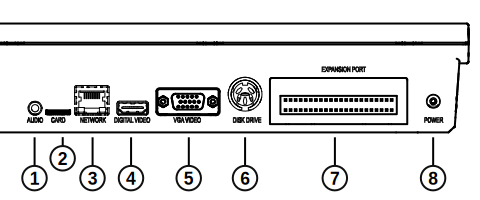
\includegraphics[width=\linewidth]{images/illustrations/mega65-rear.pdf}
\begin{center}
\setlength{\def\arraystretch{1.5}\tabcolsep}{6pt}
\begin{longtable}{ c | l}
	1	& 	3.5mm Audio Jack \\
	2	& 	External microSD Card Slot\\
	3	& 	Network LAN Port \\
	4	& 	Digital Video Connector (including sound) \\
	5	& 	VGA Video Connector \\
	6	& 	IEC Serial Bus Connector for Disk Drives and Printers \\
	7	& 	Cartridge Expansion Port \\
	8	& 	Power Supply Socket \\
\end{longtable}
\end{center}

\vspace{-1cm}

\section{Side Connections}

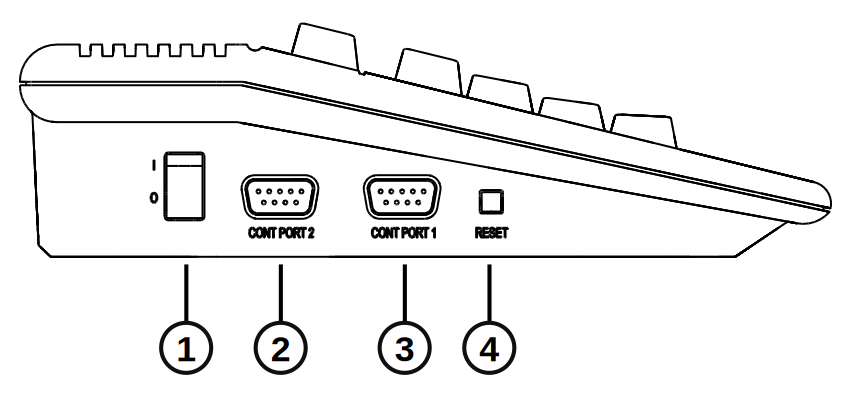
\includegraphics[width=\linewidth]{images/illustrations/mega65-side.pdf}

\begin{center}
\setlength{\def\arraystretch{1.5}\tabcolsep}{6pt}
\begin{longtable}{ c | l}
	1	& 	Power Switch \\
	2	& 	Controller Port 2 \\
	3	& 	Controller Port 1 \\
	4	& 	Reset Button \\
\end{longtable}
\end{center}

Various peripherals can be connected to Controller Ports 1 and 2 such as
joysticks, paddles or mouse devices.

\newpage

\section{MEGA65 Screen and Peripherals}

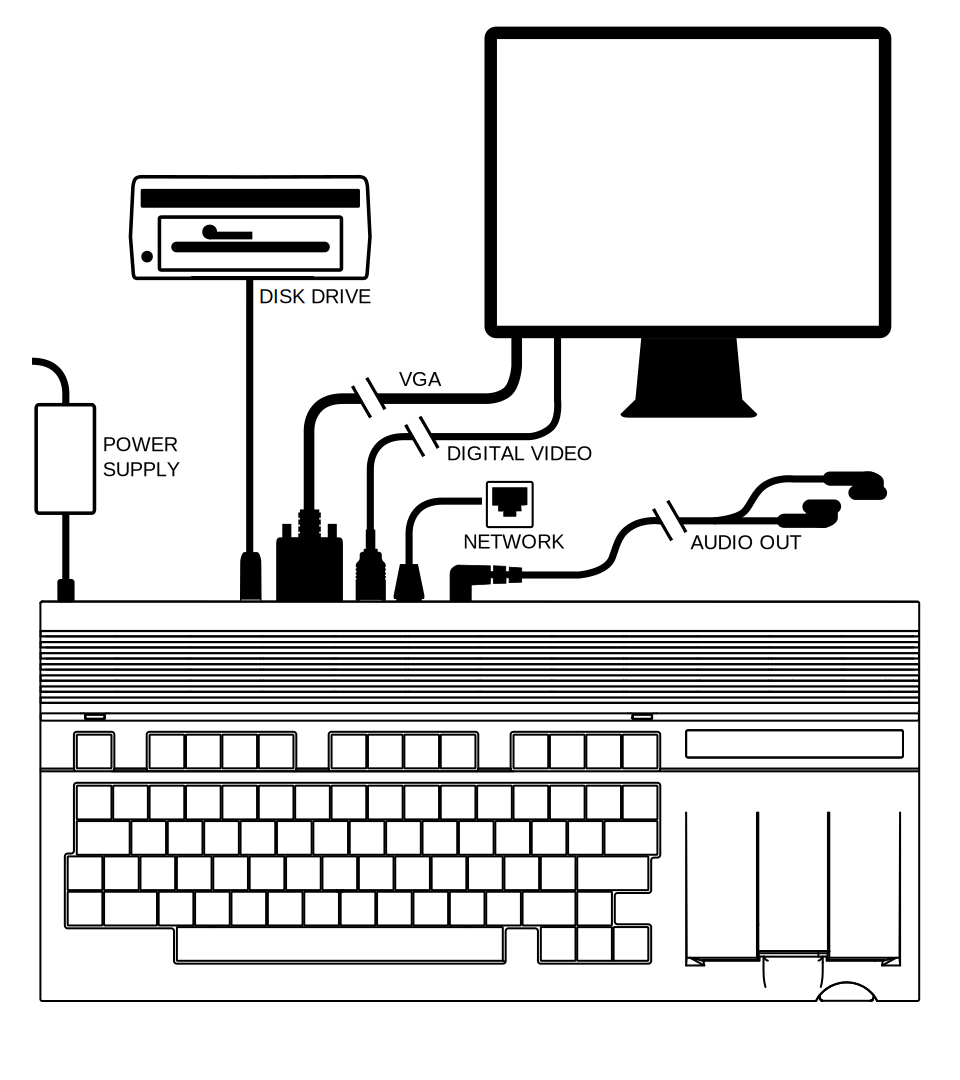
\includegraphics[width=\linewidth]{images/illustrations/mega65-top.pdf}

To connect your MEGA65 to a display:
\index{Display!Connecting}

\begin{enumerate}
	\item Connect the power supply to the power supply socket of the MEGA65.
	\item If you have a VGA monitor and a VGA cable, connect one end to the VGA port of the MEGA65 and the other end into your VGA monitor.
	\item If you have a TV or monitor with a compatible Digital Video connector,\footnote{The Digital Video connector type has a recognizable four-letter commercial name, but the MEGA65 project has not paid the licensing fees to refer to it by this name. This {\em User's Guide} refers to this as the ``Digital Video'' connector.}\index{Digital Video} connect one end of your cable to the Digital Video port of the MEGA65, and the other into the Digital Video port of your monitor. If you own a monitor with a DVI socket, you can use a Digital Video to DVI adapter.
\end{enumerate}

\newpage
\section{Optional Connections}
\index{Disk Drives!Connecting}
\index{Connections!IEC}
\index{SD Cards!Locations}
\begin{enumerate}
	\item The MEGA65 includes an internal 3.5" floppy disk drive. You can also connect older Commodore{\textregistered} IEC serial floppy drives to the MEGA65, such as the Commodore 1541, 1571 or 1581. To use these drives, connect one end of an IEC cable to the Commodore floppy disk drive and the other end to the Disk Drive socket of the MEGA65. You can also connect an SD2IEC device\index{SD2IEC device} or a Pi1541 device.\index{Pi1541 device} With most devices, you can daisy-chain additional floppy disk drives or Commodore compatible printers.
	\item You can connect your MEGA65 to an Ethernet network using a standard Ethernet cable.
	\item For enjoying audio from your MEGA65, you can connect a 3.5mm audio jack cable to an audio amplifier or speaker system. If your system has RCA connectors you will need a 3.5mm audio jack to twin RCA adapter cable. The MEGA65 also has a built-in amplifier to allow the use of headphones.
	\item A microSD card, type SDHC between 4GB and 32GB, can be inserted into the external microSD card slot at the rear of the MEGA65. For more information on using the microSD card slot, see ``Introducing SD Cards'' on page \pageref{sec:introducing-sd-cards}.
	\item Underneath the MEGA65, a small door provides access to the internal SD card and two connectors for future hardware expansion.
\end{enumerate}

\index{Real-Time Clock!Installing the Battery}
\subsection{Installing the Real-Time Clock Battery}

The MEGA65 includes a Real-Time Clock, which is used to display the time and date on the startup screen, to add timestamps to files that the MEGA65 writes to your SD cards, and by the {\bf DT\$}\index{BASIC 65 Variables!DT} and {\bf TI\$}\index{BASIC 65 Variables!TI\$} BASIC65 variables. This clock utilises a CR2032 coin-cell battery\footnote{Early models of MEGA65 with the "R3A" board revision used a battery of type CR1220 for the Real-Time Clock. Revisions "R5" and later, which began shipping in late 2023, use a CR2032 battery.} to keep time when the MEGA65 isn't switched on. The MEGA65 does not include a battery in order to avoid issues related to shipping batteries internationally.

To install the battery, use a Phillips-head screwdriver to open the case, exposing the motherboard.\index{Case!Opening} The case is held together with three screws, all of which are along the bottom of the front side of the case. Once the screws have been removed, carefully lift the top half of the case. Note the orientation of the keyboard connector, then disconnect it.

The battery is located between the controller ports and the keyboard connector.

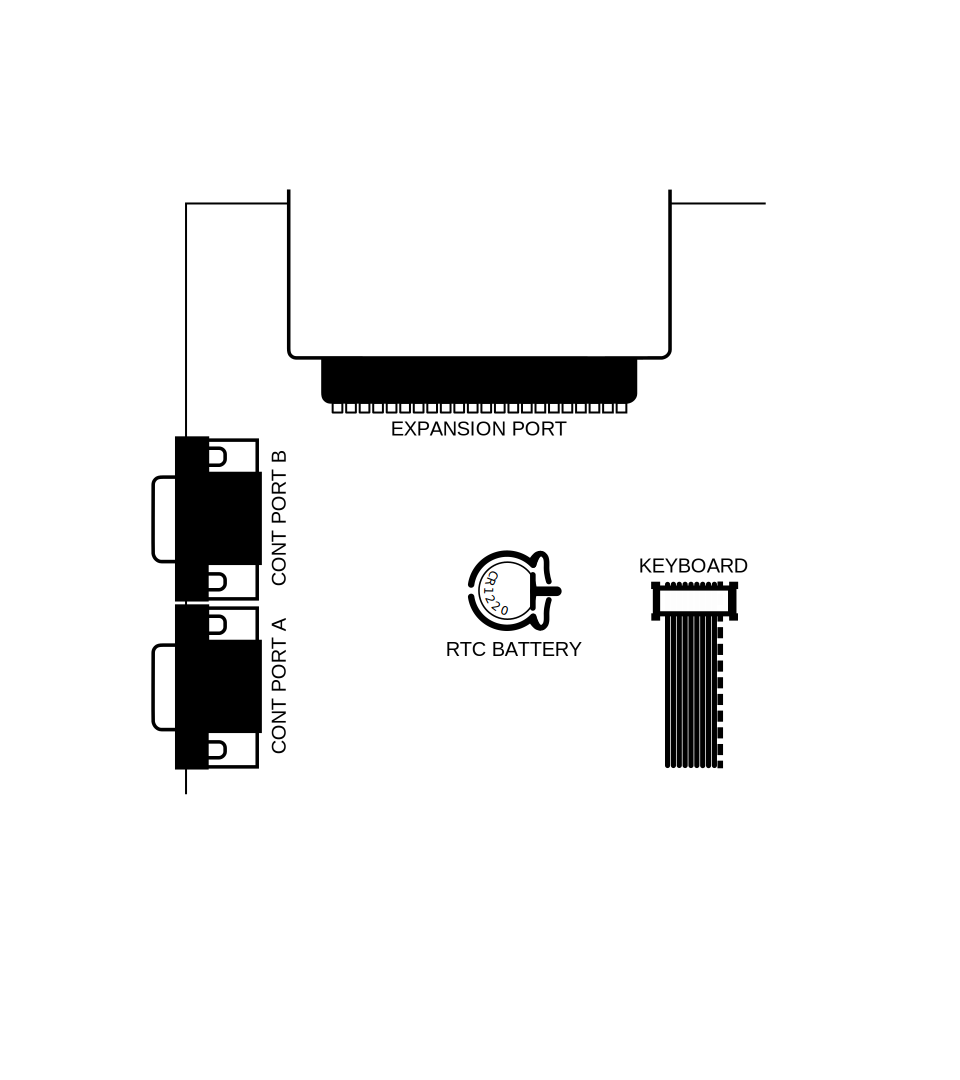
\includegraphics[width=\linewidth]{images/illustrations/rtc-battery-location.pdf}

If you are removing an existing battery, push the battery release lever on the bottom (flat-sided) side of the battery socket away from the battery to remove it. Insert the new battery with the side labelled {\bf +} facing up, and press it into place.

Once you have re-assembled your MEGA65, you can set the time in the Configuration Utility. For more information on how to set the Real-Time Clock, refer to the Configuration Utility section on page \pageref{sec:configuration-utility}.


\newpage

\section{Switching the MEGA65 on for the First Time}
\label{onboarding}

Switch the MEGA65 on using the power switch on the left-hand side of the computer.

When you switch your MEGA65 on for the first time, it displays the initial configuration (``on-boarding'') screen.\index{Configuration!On-boarding} You can use this screen to set the time and date on the Real-Time Clock (if you have installed the CR2032 battery), change the video display mode, and test the audio. All of these settings can be changed later.

\begin{center}
  \includegraphics[width=0.7\linewidth]{images/img011_final_boot_01.png}
\end{center}

For video display modes, you can select between PAL\index{PAL display mode} or NTSC\index{NTSC display mode} emulation, and you can select whether your Digital Video display supports sound. If you are using the VGA video output, the Digital Video sound mode has no effect.

\underline{Note}: A DVI display that does not support sound will not work with the ``enhanced'' sound mode. With such a display, you must select a video mode with ``no sound,'' and connect a speaker to the 3.5 mm audio jack.

PAL and NTSC are analog video signal formats that affect the resolution and vertical sync speed of the video output, even when using a modern digital display. Your display may support either mode, or it may only support one or the other. You can use this screen to test the modes with your display.

Select and test your video configuration. For example, press \specialkey{TAB} to switch to the {\bf PAL 50HZ} mode.
\index{Display!Setting PAL/NTSC}
\begin{center}
  \includegraphics[width=0.7\linewidth]{images/img011_final_boot_02.png}
\end{center}

Press \megakey{SPACE} followed by \megakey{Y} to test the new video mode.

\begin{center}
  \includegraphics[width=0.7\linewidth]{images/img011_final_boot_03.png}
\end{center}

Press \megakey{K} to keep the new video mode.

\begin{center}
  \includegraphics[width=0.7\linewidth]{images/img011_final_boot_04.png}
\end{center}

Take this opportunity to test your sound set-up. Press \megakey{A} to play a sound.

The ``CRT emulation'' option is a fun choice when using a modern flat panel display. It adds vertical gaps between pixels to simulate the CRT raster line. Try it to see if you like it: press the \megakey{C} key to toggle it on and off.

Finally, press \specialkey{RETURN} to complete the configuration.

For more information about configuring your MEGA65, see chapter \vref{cha:configuringyourmega}.

\section{The Intro Disk}
\index{Intro Disk}

After completing the on-boarding configuration, your MEGA65 starts the Intro Disk menu. The Intro Disk is a collection of software made by the MEGA65 community that demonstrates some of the capabilities of the computer. Take some time to browse the menus and try some of the demos. After each demo, press the reset button on the left-hand side of the computer to return to the Intro Disk menu.

\begin{center}
  \includegraphics[width=0.7\linewidth]{images/demo_title.png}
\end{center}

By default, the Intro Disk menu opens each time you switch on the computer. Once you are more familiar with the MEGA65, you may wish to disable this. Press \megakey{D} at the Intro Disk menu to disable its auto-boot feature.\index{Intro Disk!Disabling}

Press \megakey{X} to exit the Intro Disk menu and access BASIC 65. With the Intro Disk auto-boot feature disabled, the MEGA65 goes directly to BASIC 65 when you switch it on.

\begin{center}
  \includegraphics[width=0.7\linewidth]{images/img011_final_boot_06.png}
\end{center}

\section{The Cursor}

The flashing square underneath the \screentext{READY} prompt\index{READY prompt} is called the cursor. The cursor indicates that the computer is ready to accept input. Pressing keys on the keyboard will print their respective characters onto the screen. The characters will be printed at the current cursor position, and the cursor will advance to the next position after every key press.

Here you can type commands, that can do things such as loading a program. You can also start entering program code!

\chapter{Getting Started}
\addtocontents{toc}{\protect\setcounter{tocdepth}{2}}
\hypersetup{bookmarksdepth=5}

\section{Keyboard}
\label{cha:getting-started}
\index{Keyboard}

Now that everything is connected, it's time to get familiar with the MEGA65 keyboard.

You may notice that the keyboard is a little different to the keyboards used on computers today. While most keys will be in familiar positions, there are some specialised keys, and some with special graphic symbols marked on the front.

The graphic symbols are typable in some display modes, similar to letters, numbers, and punctuation. The complete set of characters is known as the {\em PETSCII character set}.\index{PETSCII}

\subsection{Special Keys}

\subsubsection{RETURN}
\index{Keyboard!RETURN}
Pressing \specialkey{RETURN} enters the information you have typed into the MEGA65's memory. The computer will either act on a command, store some information, or display an error message if you made a mistake.

\subsubsection{SHIFT}
\index{Keyboard!Shift Keys}
The two \specialkey{SHIFT} keys are located on the left and the right. They work very much like the Shift key on a regular keyboard. They also perform some special functions as well.

In upper case mode, holding down \specialkey{SHIFT} and pressing any key with two graphic symbols on the front produces the right-hand symbol on that key. For example, \specialkey{SHIFT} and \megakey{J} prints the \graphicsymbol{J} character.

In lower case mode, pressing \specialkey{SHIFT} and a letter key prints the upper case letter on that key.

Finally, holding \specialkey{SHIFT} down and pressing a Function key accesses the function shown on the front of that key. For example: \specialkey{SHIFT} and \megakey{F1} activates \megakey{F2}.


\subsubsection{SHIFT LOCK}
\index{Keyboard!SHIFT LOCK}
In addition to \specialkey{SHIFT} is \specialkey{SHIFT\\LOCK}. Press this key to lock down the Shift function. Now any key you press while \specialkey{SHIFT\\LOCK} is illuminated prints the character to the screen as if you were holding down \specialkey{SHIFT}. This includes special graphic characters.

\subsubsection{CTRL}
\index{Keyboard!CTRL}
\specialkey{CTRL} is the Control key. Holding down \specialkey{CTRL} and pressing another key allows you to perform Control functions. For example, holding down \specialkey{CTRL} and one of the number keys (from \megakey{1} to \megakey{8}) allows you to change text colours. The colour that is printed at the top row on the front of the number key will be used. Holding down \specialkey{CTRL} and pressing \megakey{9} or \megakey{0} switches reverse-text mode on and off.

There are some examples of this on page \pageref{sec:screen-editor}, and all of the Control functions are listed on page \pageref{appendix:controlcodes}.

If a program is being {\bf LIST}ed to the screen, holding down \specialkey{CTRL} slows down the display of each line. You can read more about the {\bf LIST} command on page \pageref{BASIC 65 Commands!LIST}.\index{BASIC 65 Commands!LIST}

Holding \specialkey{CTRL} and pressing \megakey{*} enters the Matrix Mode Debugger (refer to the {\bf MEGA65 Book} for more details).

\subsubsection{RUN STOP}
\index{Keyboard!RUN STOP}
Normally, pressing \specialkey{RUN STOP} stops the execution of a program. Holding \specialkey{SHIFT} while pressing \specialkey{RUN STOP} {\bf RUN}s the first program from disk.\index{BASIC 65 Commands!RUN}

Some programs override the \specialkey{RUN STOP} key and cannot be stopped in this way.

You can boot your MEGA65 into the {\bf Machine Code Monitor}\index{Machine Code Monitor} by holding down \specialkey{RUN STOP} and pressing reset on the left-hand side.

\subsubsection{RESTORE}
\index{Keyboard!RESTORE}
The computer screen can be restored to a clean state without clearing the memory by holding down \specialkey{RUN STOP} and pressing \widekey{RESTORE}. This combination also resets operating system vectors and re-initialises the screen editor, which makes it a handy combination if the computer has become a little confused.

Some programs override the \specialkey{RUN STOP} + \widekey{RESTORE} key combination and cannot be reset in this way.

You can also enter the {\bf Freezer} by pressing and holding \widekey{RESTORE} for half to one second. You can
read more about the Freezer on page \pageref{sec:freezer}.\index{Freezer menu}

\subsubsection{THE CURSOR KEYS}
\index{Keyboard!Cursor Keys}
\nopagebreak
At the bottom right-hand side of the keyboard are the cursor keys. These four directional keys allow you move the cursor to any position for on-screen editing.

The cursor moves in the direction indicated on the keys: \megakey{$\leftarrow$} \megakey{$\uparrow$} \megakey{$\rightarrow$} \megakey{$\downarrow$}.

You don't have to keep pressing a cursor key over and over. If you need to move the cursor a long way, you can keep the key pressed down. When you are finished, simply release the key.

\subsubsection{ARROW KEYS}
\index{Keyboard!Arrow Keys}
These keys are different to the cursor keys! They are \megakeywhite{$\leftarrow$} (next to \megakey{1}), and \megakeywhite{$\uparrow$} (next to \widekey{RESTORE}).
Both arrow keys are used in various BASIC functions and escape sequences.

For example, \megakeywhite{$\leftarrow$} can be used as a shortcut for {\bf SAVE},\index{BASIC 65 Commands!SAVE} and \megakeywhite{$\uparrow$} is used to raise a number to a power (which is the same as multiplying a number by itself a specified number of times).

You can read more about the available escape sequences on page \pageref{escape-sequences}.

These two PETSCII specific keys will always be shown in MEGA65 literature with a white background.

It is also possible to move the cursor up by using \specialkey{SHIFT} and \megakey{$\downarrow$}, and left by using \specialkey{SHIFT} and \megakey{$\rightarrow$}. This owes to the MEGA65's Commodore 64 heritage, which only had two cursor keys.

\subsubsection{INSerT/DELete}
\index{Keyboard!INST DEL}
This is the INSERT / DELETE key. When pressing \specialkey{INST\\DEL}, the character to the left is deleted, and all characters to the right are shifted one position to the left.

To insert a character, hold \specialkey{SHIFT} and press \specialkey{INST\\DEL}. All the characters to the right of the cursor are shifted to the right. This allows you to type a letter, number or any other character at the newly inserted space.


\subsubsection{CLeaR/HOME}
\index{Keyboard!CLR HOME}
Pressing \specialkey{CLR\\HOME} places the cursor at the top left-most position of the screen.

Holding down \specialkey{SHIFT} and pressing \specialkey{CLR\\HOME} clears the entire screen {\it and} places the cursor at the top left-most position of the screen.

If you press \specialkey{CLR\\HOME} accidentally, you can return the cursor to its prior position by pressing \specialkey{ESC} then \specialkey{CLR\\HOME}.

\subsubsection{MEGA KEY}
\index{Keyboard!MEGA Key}
\megasymbolkey or the MEGA key provides a number of different functions and can be used to launch special utilities.

Holding \specialkey{SHIFT} and pressing \megasymbolkey switches between lower and uppercase character modes.

Holding \megasymbolkey and pressing any key with two graphic symbols on the front prints the left-most graphic symbol to the screen. For example,
\megasymbolkey and \megakey{D} prints the \graphicsymbol{d} symbol.

Holding \megasymbolkey and pressing any key that shows a single graphic symbol on the front prints that graphic symbol to the screen.

Holding \megasymbolkey and pressing a number key switches to one of the colours in the second range, i.e., the colour that is printed at the bottom row on the front of the number key will be used.

Holding \megasymbolkey and pressing \specialkey{TAB} enters the Matrix Mode Debugger (refer to the {\bf MEGA65 Book} for more details).

Switching on the MEGA65 or pressing the reset button on the left-hand side while holding down \megasymbolkey switches the MEGA65 into GO64 mode.\index{Commodore 64!GO64 mode}

\subsubsection{NO SCROLL}
\index{Keyboard!NO SCROLL}
If a program is being {\bf LIST}ed to the screen, pressing \specialkey{NO\\SCROLL} pauses the screen output. Press any key to un-pause.

This feature is not available in GO64 mode.\index{Commodore 64!GO64 mode}

\subsubsection{FUNCTION KEYS}
\index{Keyboard!Function Keys}
There are seven Function keys available for use by software applications. \megakey{F1} \megakey{F3} \megakey{F5} \megakey{F7} \megakey{F9} \megakey{F11} and \megakey{F13} can be used to perform special functions.

Hold \specialkey{SHIFT} to access \megakey{F2} through to \megakey{F14} as shown on the front of each Function key.
\index{Keyboard!Shift Keys}
Only Function keys \megakey{F1} to \megakey{F8} are available in GO64 mode.\index{Commodore 64!GO64 mode}

\subsubsection{HELP}
\index{Keyboard!HELP}
\specialkey{HELP} can be used by software and also acts as \megakey{F15} / \megakey{F16}.

\subsubsection{ALT}
\index{Keyboard!ALT}
Holding \specialkey{ALT} down while pressing other keys can be used by software to perform specific functions. This feature is not available in GO64 mode.\index{Commodore 64!GO64 mode}

Holding \specialkey{ALT} down while switching the MEGA65 on activates the Utility Menu.\index{Utility menu} You can format an SD card, or enter the MEGA65 Configuration Utility\index{Configuration!Utility} to select the default video mode and change other settings, or to test your keyboard.

\subsubsection{CAPS LOCK}
\index{Keyboard!CAPS LOCK}
\specialkey{CAPS\\LOCK} works similarly to \specialkey{SHIFT\\LOCK} in C65 and MEGA65-modes, but only modifies the letter keys.

When the MEGA65 is set to run at a reduced processor speed, such as in GO64 mode,\index{Commodore 64!GO64 mode} you can hold down \specialkey{CAPS\\LOCK} to run the processor at full speed temporarily. This is useful in GO64 mode for things such as
speeding up loading from the internal disk drive or SD card, or to greatly speed up the de-packing process after a program is run. MEGA65 mode runs at maximum speed by default.

\addtocontents{toc}{\protect\setcounter{tocdepth}{5}}


\section{The Screen Editor}
\label{sec:screen-editor}

When you switch on your MEGA65 or reset it, the following screen will appear:\footnote{This assumes you have disabled the Intro Disk menu. If the Intro Disk menu is running, press ``X'' to exit to this screen.}

\begin{center}
\includegraphics[width=0.9\linewidth]{images/introduction-screen/layout.png}
\end{center}

The colour bars in the top left-hand side of the screen can be used as a guide to help calibrate the colours of your display. The screen also displays the name of the system, the copyright notice, and the ROM version. The displayed date and time are taken from the internal RTC (Real-Time Clock) at the time the computer was powered on. You can set the date and time in the Configure Utility.

Finally, you will see the \screentext{READY} prompt and the flashing cursor.

You can begin typing keys on the keyboard and the characters will be printed at the cursor position. The cursor itself will advance after each key press.

You can also produce reverse text or colour bars by holding down \specialkey{CTRL} and pressing \megakey{9}, or \megakey{R}. This enters reverse text mode. When this is enabled, you can press and hold the \megakey{Space} bar. While doing so, a white bar will be drawn across the screen.
\index{Keyboard!CTRL}
You can change the current colour by holding \specialkey{CTRL} down and pressing a number key (from \megakey{1}
to \megakey{8}). For example, if you press and hold \specialkey{CTRL} down and press \megakey{1}, the colour will
change to black. Now, when you hold down the \megakey{Space} bar, a black bar will be drawn. If you continue to
change the colour and press the \megakey{Space} bar, you will get an effect similar to the following image:

\begin{center}
\includegraphics[width=0.7\linewidth]{images/introduction-screen/colour-bars.png}
\end{center}

You can disable reverse text mode by holding \specialkey{CTRL} and pressing \megakey{0}.

A further eight colours can be selected by holding down \megasymbolkey and pressing a key from \megakey{1} to \megakey{8}.\index{Keyboard!MEGA Key}

The colour that is printed at the bottom row on the front of the number key will be used. For example, if you held
\megasymbolkey down while pressing \megakey{4}, dark grey will be used. For access to an additional 16 colours of the alternate/rainbow palette, refer to the \specialkey{CTRL} + \megakey{A} shortcut described on page \pageref{appendix:controlcodes}.

\underline{NOTE}:
\begin{itemize}
  \item {\bf Quote Mode}: If you were to press \megakey{"} to open a string, and then try to change
colours, reverse text, move the cursor keys, or use the \specialkey{CLR HOME} key, instead
of these actions instantly occurring, funny PETSCII\index{PETSCII} symbols will appear instead. This is
due to a BASIC facility called {\it quote mode} (described further in the \textbf{MEGA65 Book}),
which allows you to encode such actions into a string so that they can be executed at a later
time (for example, via a {\bf PRINT} statement within your programs). To end {\it quote mode}, simply
type another \megakey{"} to mark the end of your string.
  \item {\bf Insert Mode}: A similar facility is called
{\it insert mode}, where for the number of times you press \specialkey{SHIFT} + \specialkey{INST\\DEL}
to insert a few spaces, the same number of keypresses that follow it will abide by the same
principles of {\it quote mode}.
  \item You can forcefully exit either of these modes by pressing \specialkey{ESC}, \megakey{O}.
\end{itemize}

\needspace{4cm}
You can create fun pictures just by using these colours and letters. Here's an example of what a 4th year student drew:

\begin{center}
\includegraphics[width=0.7\linewidth]{images/caleb-PETSCII-TNT-final}
\end{center}

What will you draw?

\needspace{2cm}
\textbf{Functions}

Functions using \specialkey{CTRL} are called \textbf{Control Codes}.
Functions using \megasymbolkey are called \textbf{Mega Codes}. There are also functions that are called by using \specialkey{SHIFT}, which are called \textbf{Shifted Codes}.

Lastly, \specialkey{ESC} enables the use of \textbf{Escape Sequences}.

You can read about all of these functions in detail on page \pageref{appendix:controlcodes}.

\needspace{2cm}
\textbf{ESC Sequences}

\index{Keyboard!Escape Sequences}
Escape sequences are performed a little differently than a Control function or a Shift function. Instead of holding the modifier key down, an Escape sequence is performed by pressing \specialkey{ESC} and releasing it, followed by pressing the desired key.

For example: to switch between 80 column mode and 40 column mode, press and release \specialkey{ESC}, then press \megakey{X}.

There are more text modes available. You can create flashing text by holding \specialkey{CTRL} down and pressing \megakey{O}. Any characters you type in will flash. Turn flash mode off by pressing \specialkey{ESC}, then \megakey{O}.


\section{Editor Functionality}

The MEGA65 screen editor\index{Screen editor} supports several ways to quickly move the cursor around the screen to help you to be more productive.

For example, press \specialkey{CLR HOME} to go to the home position on the screen. Hold \specialkey{CTRL} down and press \megakey{W} several times. This is the \textbf{Word Advance function}, which jumps your cursor to the next word, or printable character.

You can set custom tab positions on the screen for your convenience. Press \specialkey{CLR HOME} and then \megakey{$\rightarrow$} to move the cursor to the fourth column. Hold down \specialkey{CTRL} and press \megakey{X} to set a tab. Move another 16 positions to the right, and press \specialkey{CTRL} and \megakey{X} again to set a second tab.

Press \specialkey{CLR HOME} to go back to the home position. Hold \specialkey{CTRL} down and press \megakey{I}. This is the \textbf{Forward Tab function}. Your cursor will tab to the fourth position. Press \specialkey{CTRL} and \megakey{I} again. Your cursor will move to position 8. By default, every 8th position is already set as a tabbed position. So the 4th and 20th positions have been added to the existing tab positions. You can continue to press \specialkey{CTRL} and \megakey{I} to advance to the 16th and 20th positions.

\subsection{Creating a Window}
\index{Keyboard!Escape Sequences}
\index{Windows!Escape sequences}

You can set a window on the MEGA65 working screen. Move your cursor to the beginning of the "BASIC 65" text. Press \specialkey{ESC}, then press \megakey{T}. Move the cursor 10 lines down and 15 to the right.

Press \specialkey{ESC}, then \megakey{B}. Anything you type will be contained within this window.

For example, if you were to type \screentext{LIST} to list out a program, the listing will be confined to the window region you have specified:

\begin{center}
\includegraphics[width=0.7\linewidth]{images/set-window.png}
\end{center}

To escape from the window back to the full screen, press \specialkey{CLR HOME} twice.

\subsection{Additional ASCII characters}

You may have noticed a few ASCII characters on the MEGA65 keyboard that aren't traditionally a part of the PETSCII character set.\index{PETSCII} In order to make use of these from within BASIC:

\begin{itemize}
  \item Type either \screentext{FONT A} or \screentext{FONT B}.
  \item Press \megasymbolkey + \specialkey{SHIFT} to switch to lowercase.
\end{itemize}

You will now be able to type those additional ASCII characters via the keyboard. To revert back to the original PETSCII character set, type \screentext{FONT C}.

\subsection{Uppercase and lowercase}

\megasymbolkey + \specialkey{SHIFT} switches between uppercase and lowercase text for the entire display. This works even during program execution, so you can adjust it if a program is in the wrong mode.


\section{The Freezer Menu}
\label{sec:freezer}
\index{Freezer menu}
\nopagebreak
The MEGA65 spends most of its time behaving as a Commodore 65 computer would, either running a program or awaiting instructions in the BASIC environment. Your MEGA65 has additional features that were not part of the original C65 design. You can access many of these features from the Freezer menu.

To open the Freezer menu, hold the \widekey{RESTORE} key for one second, then release it. The MEGA65 will pause whatever it is doing, flicker the border colour, then open the Freezer menu. Whatever program was running remains in memory and can be resumed by pressing the \specialkey{F3} key. You can also abandon the running program and reset the MEGA65 by pressing \specialkey{F5}.

\begin{center}
  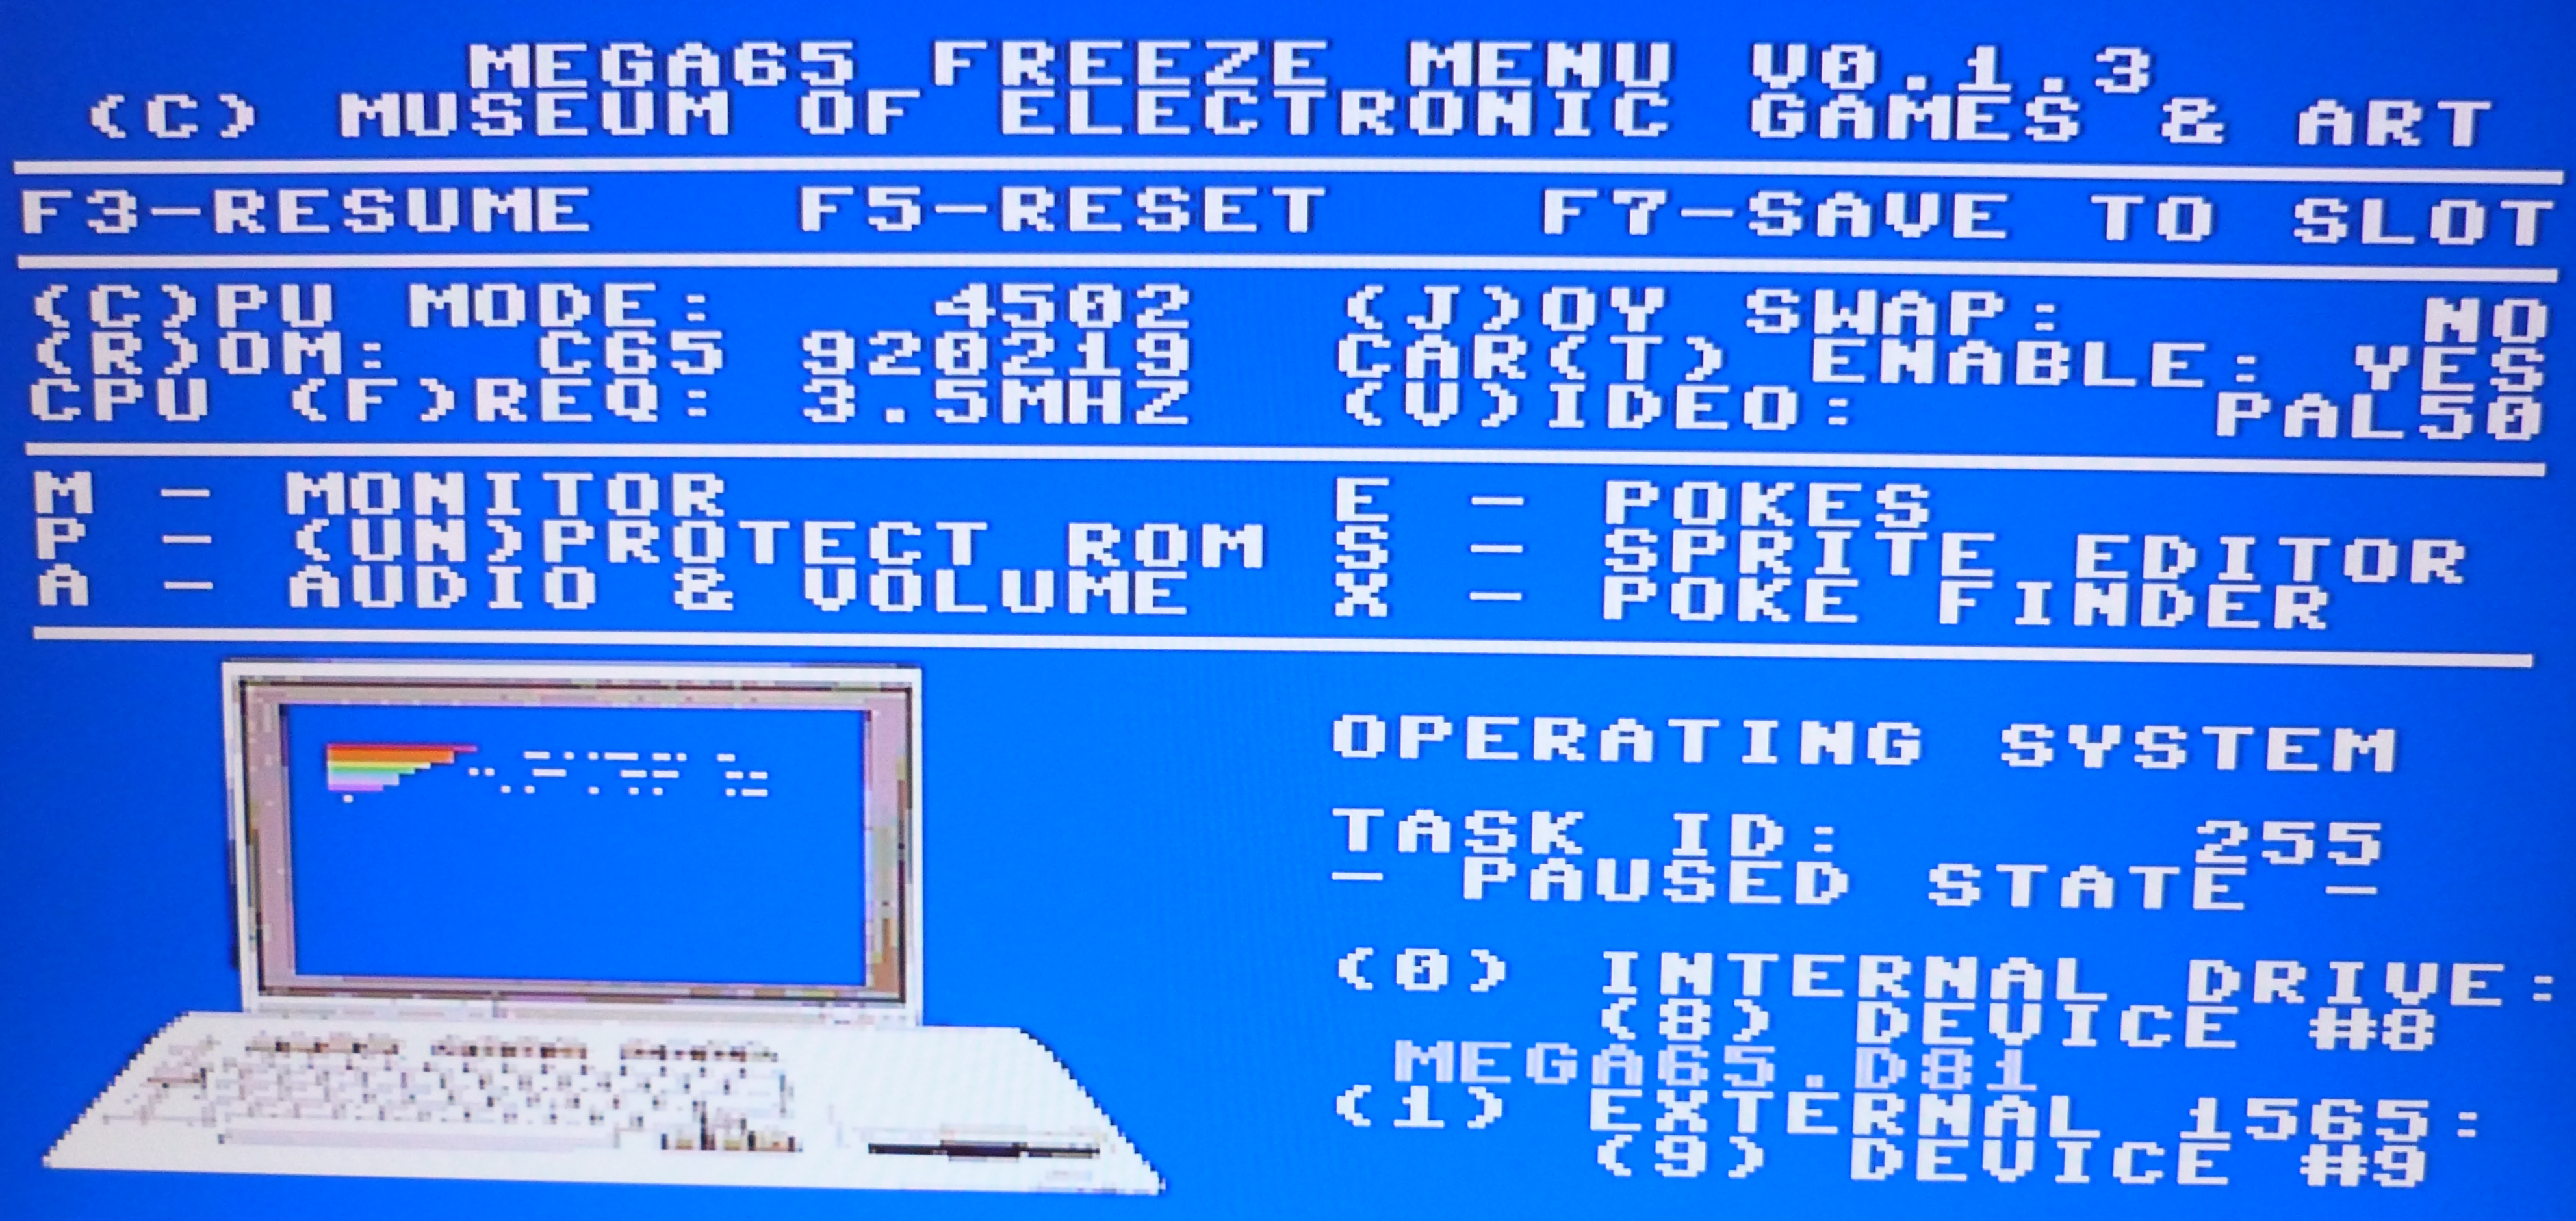
\includegraphics[width=0.7\linewidth]{images/freezer.png}
\end{center}

One feature to remember when playing games is the ``(J)OY SWAP.'' This causes the two joystick ports to trade numbers. If you have a joystick in port 2 and you start a game that expects a joystick in port 1, instead of disconnecting and reconnecting the joystick, open the Freezer menu, press \megakey{J} to swap the port numbers, then resume your game.

This is called the ``Freezer'' menu because the state of the MEGA65 remains frozen while using it. The Freezer menu can store multiple freeze states, and you can switch between them. To save the current state, navigate to an unused {\it freeze slot} using the cursor-right key, then press \megakey{F7}. When the border stops blinking, the state is saved. To restore a state, navigate to the freeze slot, then press \megakey{F3} to resume operation.

The Freezer menu has several built-in options and features. For more information about the MEGA65 Information Utility (``MEGAINFO''), see ``Determining the Versions of Things'' on page \pageref{sec:versions}. For more information about mounting disks and disk images, see chapter \vref{cha:using-disks}.


\section{Running Commodore 64 Software}

The MEGA65 is capable of running Commodore 64 software. There are two ways to do this: the built-in GO64 mode, and the {\it C64 for MEGA65} FPGA core.

\subsection{GO64 Mode}
\index{Commodore 64!GO64 mode}

The original Commodore 65 was designed to be capable of running some Commodore 64 software. The MEGA65 supports this feature, known as ``GO64 mode.''

\underline{NOTE}: Due to how Commodore designed this feature, not all C64 software is compatible with this mode. Unlike the similar feature of the Commodore 128, the Commodore 65 uses a different CPU, and minor differences are known to cause compatibility issues with some software titles.

There are three ways to switch the MEGA65 into GO64 mode:

\begin{itemize}
    \item Switch off the computer, hold the \megasymbolkey and switch it back on.
    \item From the MEGA65 \screentext{READY} prompt, enter this command: \screentext{GO64} Enter \screentext{YES} when prompted.\index{BASIC 65 Commands!GO64}
    \item Switch off the computer, connect a Commodore 64 cartridge to the expansion port, then switch the computer on.
\end{itemize}

\begin{center}
  \includegraphics[width=0.7\linewidth]{images/go64.png}
\end{center}

GO64 mode is actually just a temporary re-configuration of the MEGA65. All of the MEGA65's features are still present, including the Freezer menu for mounting D81 disk images.

Much Commodore 64 software can be found on the Internet in the form of D64 disk images. The MEGA65 only supports D81 disk images via the SD card and Freezer menu. You can use a peripheral such as the SD2IEC\index{SD2IEC device} with the MEGA65's IEC port to use D64 disk images. Be sure to obtain an SD2IEC with an independent power supply, and not one that depends on a Commodore 64 tape connector.\footnote{For more information on SD2IEC devices, see: \url{https://www.c64-wiki.com/wiki/SD2IEC}}

\subsection{The ``C64 for MEGA65'' FPGA Core}
\index{Core!C64 core}\index{Commodore 64!Core}

The {\it C64 for MEGA65} FPGA core by MJoergen and sy2002 re-creates the original Commodore 64 computer on MEGA65 hardware with a high degree of accuracy. It does so by completely replacing the MEGA65 core with one that implements the Commodore 64 chipset, including its CPU. MEGA65 features such as the Freezer menu are not available when running the C64 core. Instead, the core provides its own menu for mounting D64 disk images and other features. Press the \specialkey{HELP} key with the core running to access this menu.

% TODO: When the cartridge-to-core configuration feature is complete:
% With the C64 core installed, you can configure the MEGA65 boot process to use the core when a Commodore 64 cartridge is connected, instead of using the less-compatible GO64 mode. ...
% (Refer to chapter \vref{cha:cores})

For information about installing FPGA cores, see chapter \vref{cha:cores}. To download the {\it C64 for MEGA65} core and read important installation instructions, see: \url{https://github.com/MJoergen/C64MEGA65}

\section{The Screen Editor}
\label{sec:screen-editor}

When you switch on your MEGA65 or reset it, the following screen will appear:

\begin{center}
\includegraphics[width={10cm}]{images/introduction-screen/layout.png}
\end{center}

The colour bars in the top left-hand side of the screen can be used
as a guide to help calibrate the colours of your display.
The screen also displays the name of the system,
the copyright notice, and the ROM version.
The displayed date and time are taken from the internal RTC
(Real-Time Clock), which can be set in the Configure Menu.

Finally, you will see the \screentext{READY} prompt and the flashing cursor.

You can begin typing keys on the keyboard and the characters will be
printed at the cursor position. The cursor itself will advance after
each key press.

You can also produce reverse text or colour bars by holding down \specialkey{CTRL} and pressing \megakey{9}, or \megakey{R}. This enters reverse text mode. When this is enabled, you can press and hold the \megakey{Space} bar. While doing so, a white bar will be drawn across the screen.
\index{Keyboard!CTRL}
You can even change the current colour by holding \specialkey{CTRL} down and pressing a number key (from \megakey{1} to \megakey{8}). For example, if you press and hold \specialkey{CTRL} down and press \megakey{1}, the colour will change to black. Now, when you hold down the \megakey{Space} bar, a black bar will be drawn. If you continue to change the colour and press the \megakey{Space} bar, you will get an effect similar to the image below:


\begin{center}
\includegraphics[width={10cm}]{images/introduction-screen/colour-bars.png}
\end{center}


\index{Keyboard!MEGA Key}
You can disable reverse text mode by holding \specialkey{CTRL} and pressing \megakey{0}.

By pressing any key, characters will be printed to the screen in the chosen colour.

A further eight colours can be selected by holding down \megasymbolkey and pressing a key from \megakey{1} to \megakey{8}.
The colour that is printed at the bottom row on the front of the number key will be used. For example, if you held
\megasymbolkey down while pressing \megakey{4}, dark gray will be used. For even more colours, see \bookvref{appendix:escape-colours}.

\needspace{4cm}
You can create fun pictures just by using these colours and letters.  Here's an example of what a year four student drew:

\begin{center}
\includegraphics[width={6cm}]{images/caleb-PETSCII-TNT-final}
\end{center}

What will you draw?

\needspace{2cm}
\textbf{Functions}

Functions using \specialkey{CTRL} are called \textbf{Control Codes}.
Functions using \megasymbolkey are called \textbf{Mega Codes}. There are also functions that are called by using \specialkey{SHIFT}, which
are called \textbf{Shifted Codes}.

Lastly, \specialkey{ESC} enables the use of \textbf{Escape Sequences}.

You can read about all of these functions in detail in \bookvref{appendix:controlcodes}, but some are shown in this section.


\needspace{2cm}
\textbf{ESC Sequences}
\index{Keyboard!Escape Sequences}
Escape sequences are performed a little differently than a Control function or a Shift function. Instead of holding the modifier key down, an Escape sequence is performed by pressing \specialkey{ESC} and releasing it, followed by pressing the desired key code.

For example: to switch between 40/80 column mode, press and release \specialkey{ESC}, then press \megakey{X}.

There are more modes available. You can create flashing text by holding \specialkey{CTRL} down and pressing \megakey{O}. Any characters you type in will flash. Turn flash mode off by pressing \specialkey{ESC},  then \megakey{O}.



\section{Editor Functionality}


The MEGA65 screen can allow you to do advanced tabbing, and quickly move around the screen in many ways to help you to be more productive.

For example, press \specialkey{CLR HOME} to go to the home position on the screen. Hold \specialkey{CTRL} down and press \megakey{W} several times. This is the \textbf{Word Advance function}, which jumps your cursor to the next word, or printable character.

You can set custom tab positions on the screen for your convenience. Press \specialkey{CLR HOME} and then \megakey{$\rightarrow$} to the fourth column. Hold down \specialkey{CTRL} and press \megakey{X} to set a tab. Move another 16 positions to the right again, and press \specialkey{CTRL} and \megakey{X} again to set a second tab.

Press \specialkey{CLR HOME} to go back to the home position. Hold \specialkey{CTRL} down and press \megakey{I}. This is the \textbf{Forward Tab function}. Your cursor will tab to the fourth position. Press \specialkey{CTRL} and \megakey{I} again. Your cursor will move to position 8. Why do you ask? By default, every 8th position is already set as a tabbed position. So the 4th and 20th positions have been added to the existing tab positions. You can continue to press \specialkey{CTRL} and \megakey{I} to advance to the 16th and 20th positions.

To find the complete set of Control codes, see \bookvref{appendix:controlcodes}.

\textbf{Creating a Window}

You can set a window on the MEGA65 working screen. Move your cursor to the beginning of the "BASIC 65" text. Press \specialkey{ESC}, then press \megakey{T}. Move the cursor 10 lines down and 15 to the right.

Press \specialkey{ESC}, then \megakey{B}. Anything you type will be contained within this window.

To escape from the window back to the full screen, press \specialkey{CLR HOME} twice.


\textbf{Extras}

Long press on \widekey{RESTORE} to go into the Freeze Menu.  Then press \megakey{J} to switch joystick ports without having to physically swap the joystick to the other port.

Go to \textbf{Fast mode} (40.5MHz) by either typing \screentext{FAST}, or \screentext{POKE 0,65} or use the Freeze Menu.

Return back to \textbf{Slow mode} (1MHz) by either typing \screentext{FAST 1}, or \screentext{POKE 0,64} or use the Freeze Menu.

\megasymbolkey + \specialkey{SHIFT} switches between uppercase and lowercase text for the entire display.

\chapter{Configuring your MEGA65}
\label{cha:configuring}

\section{Important Note}

For your convenience, your MEGA65 comes with an SD card with all of the essential
files already on it, so you may prefer to skip this section and jump straight to
the on-boarding section on page \pageref{onboarding}.

Alternatively, you're welcome to read this section and familiarise
yourself on how your SD card was prepared.

{\bf Do not format the SD card that came with your MEGA65}.
If you want to create a new bootable SD card, please use another one,
and keep the SD card that came with your MEGA65 as a safety backup.

\section{Formatting SD cards}
\index{SD Cards!Formatting}
The MEGA65 has two SD card slots: A full-size SD card slot inside, under
the trap-door, and a microSD size slot on the rear.  The current version
of the MEGA65 firmware only supports the use of one SD card at a time.
If you have cards in both slots, the MEGA65 will default to the external slot. The exception to this is that the MEGA65's FDISK/FORMAT
utility can access both, allowing you to select which SD card to format or
repair.

If you wish to use a different SD card to the pre-configured one supplied with your MEGA65, the new SD card must be formatted first.

{\bf This must be done on the MEGA65, not on a PC or other computer.}

{\em Only use SDHC cards. Older SD cards (typically with
  a capacity of <4GB) will not work. Newer SDXC cards with
  capacities greater than 32GB may or may not work. We would
  appreciate hearing your experience with such cards. It is unimportant
  as to which file-system is currently on the card, as the MEGA65
  FDISK/FORMAT utility will completely reformat the card.}

There are several reasons for this: First, to fit the most
features into the MEGA65's small operating system, it is
particular about the FAT32 file system it uses. Second, only the
MEGA65 FDISK/FORMAT utility can create a MEGA65 System Partition. The
MEGA65 System Partition holds non-volatile configuration settings for
your MEGA65, and also contains the freeze slots that make it easy to
switch between MEGA65 programs and games.

Formatting an SD card on the MEGA65 is easy. Switch the MEGA65 on while holding \specialkey{ALT} down.

This will present the MEGA65 Utility Menu, which contains a
selection of built-in utilities, similar to the following:

%\begin{wrapfigure}{l}{0.7\textwidth}
\begin{center}
\includegraphics[width=0.7\textwidth]{images/ss-utilmenu.png}
\end{center}
%\end{wrapfigure}

Note that the Utility Menu is always accessible, even if no SD card is present in both the internal and external slots.

The exact set of utilities
depends on the model of your MEGA65 and the version of the MEGA65
factory core which it is running. However, all versions include both
the MEGA65 FDISK/FORMAT utility (which is called \screentext{SDCARD FDISK+FORMAT UTILITY} in the screenshot above),
and the MEGA65 Configure utility.
Most models also include a keyboard test utility, that you can use
to test that your keyboard is functioning correctly.  This is
the same utility used in the factory when testing brand
new keyboards.

Select the number that corresponds to the FDISK/FORMAT utility.  This
will typically be 2.  The FDISK utility will start, and attempt to
detect the size of all SD cards you have installed.  If you have both
an internal and external SD card installed, it will allow you to
choose which one you wish to format. The internal SD card is bus 0,
and the external microSD card is bus 1. Note that the MEGA65 will
always attempt to boot from the external microSD card if one is
present.

For safety, when formatting we {\em strongly} recommend
that you remove any SD card or microSD card that you do not intend to
format, so that you do not accidentally destroy any data.  This is
because formatting an SD card on the MEGA65 cannot be undone, and
all data currently on the SD card {\em will be lost}.  If you
have files or data on the SD card that you wish to retain, you
should first back them up.  The contents of the FAT32
partition can be easily backed up by inserting the SD card into
another computer.  The contents of the MEGA65 System Partition,
including the contents of freeze slots requires the use of specialised
software.

You should aim to back up valuable data from your
MEGA65 on a regular basis, especially while the computer remains under
development.  While we take every care to avoid data corruption or
other mishaps, we cannot guarantee that the MEGA65 is free of bugs in
this regard.

If you have only an internal SD card, you might see a
display similar to the following:

\begin{center}
\includegraphics[trim= 10mm  7mm 10mm 10mm,clip,width=0.7\linewidth]{images/ss-m65fdisk-busselect.png}
\end{center}

Once you have selected the bus, the FDISK/FORMAT utility will ask you to confirm that you wish to delete everything:

\begin{center}
\includegraphics[trim= 10mm  7mm 10mm 15mm,clip,width=0.7\linewidth]{images/ss-m65fdisk-typesomething.png}
\end{center}

To avoid accidental loss of data, you must type \screentext{DELETE EVERYTHING} in capitals and press \specialkey{RETURN}. Alternatively, switch the MEGA65 off and on to abort this process without causing damage to your data.

It is also possible to attempt a recovery from a lost Master Boot Record error (also known as the Boot Sector), by typing \screentext{FIX MBR} instead.

The aim here is to have a correctly formatted SD card with all of the essential files stored on it so the MEGA65 can properly boot.
When switching on, the MEGA65 will search for, and boot using these files:
\begin{itemize}
\item {\tt FREEZER.M65} (Freeze Menu program)
\item {\tt AUDIOMIX.M65} (Freeze Menu audio mixer utility)
\item {\tt C64THUMB.M65} (C64 thumbnail image used in freezer)
\item {\tt C65THUMB.M65} (C65 thumbnail image used in freezer)
\item {\tt MEGA65.ROM}   (128KB ROM file)
\item {\tt MEGA65.D81} (Disk image)
\end{itemize}

Straight out of the box, the MEGA65 will only have one SD card installed, accessible via the trap-door under the case. This SD card contains all of the essential files needed to properly boot up.
If an external microSD card is also detected during boot up, the MEGA65 will give it higher priority, and will try to boot from it instead.
This means that the external microSD card needs to have the essential files on it, otherwise the MEGA65 will not boot up properly and will fall back to loading the OpenROM, which does not support all MEGA65 features.
In general, if your MEGA65 cannot boot properly and falls back to OpenROM, your boot-up screen will look similar to this:

\begin{center}
\includegraphics[trim=0 8cm 0 0,clip,width=0.7\linewidth]{images/mega65_OpenROM_boot_noSD.png}
\end{center}


\section{Installing ROM and Other Support Files}
\label{sec:installingrometc}

The MEGA65 FDISK/FORMAT utility will add a copy of the Open ROMs project's C64-compatible ROM
to your SD card, and will name it {\tt MEGA65.ROM}.

For MEGA65 owners, we have replaced this file with the latest ROM from the 'Closed ROMs'
project. It provides many improvements over the original/incomplete C65 ROMs. It contains
the operating system, BASIC 65, CBDOS and the machine language monitor BSMON.
This ROM is developed especially for the MEGA65 and can be
identified by the version number \screentext{92XXXX}.

However, you may have other ROMs that you wish to
use on your MEGA65.
You can copy as many of these as you wish onto the
SD card, just make sure that they have the {\tt .ROM} file extension.  The default ROM
should be called "{\tt MEGA65.ROM}". These files
must be 128KB in size, and use the same internal format as the ROMs
intended for the C65.  This means that the C64-mode KERNAL must be
placed at offset \$E000, a C65-mode BASIC at \$A000, and a suitable
character set at \$D000.

You can optionally name your alternate ROMs as {\tt MEGA65x.ROM}, replacing {\tt x} with a number from 0 to 9.
This allows you to quickly boot-up to your alternate ROMs by holding down a number from \megakey{0} to \megakey{9} prior
to switching on your MEGA65.

Other important support files include {\tt FREEZER.M65} and {\tt AUDIOMIX.M65}, which
allow you to use the MEGA65's integrated Freezer. More details are provided in the
'Floppy Disks, D81 Images, and the Freezer' chapter on page \pageref{cha:freezer}.

\subsection{ROM File}

\textbf{Original C65 ROMs}

You may want to source your own C65 ROM via other means.
There were many different versions created during the development of the Commodore 65,
and the MEGA65 can use any of them.  However, they will not support the advanced
features of the MEGA65, and are incomplete and buggy, as development on them ceased
due to Commodore abandoning the C65 project.

\textbf{MEGA65 Closed ROMs}

There are newer versions of the MEGA65 Closed ROM under development. These ROMs improve upon the original C65 ROMs and make better use of the extra hardware capabilities that the MEGA65 has over the original C65 hardware. These ROMs are available via the filehost (\url{https://files.mega65.org}), but only to owners of the MEGA65, who will need to login to the filehost with their credentials in order to download it. It can be located by visiting the \textbf{Files} tab and searching for "\textbf{kernal rom}":

\includegraphics[width=\linewidth]{images/latest_closed_rom.png}

\textbf{MEGA65 ROM diff files}

If you have sourced your own {\tt 911001.bin} C65 ROM and would like to patch it to the latest MEGA65 closed ROM,
we do provide patches, as the additional improvements we have made to the closed rom are open source.
These diff files are available at \url{http://mega65.org/rom-diffs}

\textbf{MEGA65 Open ROMs}

Another available option is to make use of \textbf{MEGA65 Open ROMs}. The latest version of this is always downloadable from either of the following urls:

\begin{itemize}
  \item \url{http://mega65.org/open-roms}
  \item \url{https://github.com/MEGA65/open-roms/raw/master/bin/mega65.rom}
\end{itemize}


\subsection{Support Files}

For official owners of the MEGA65 (both the devkit and the final product), visit the following url and log in with the user credentials you have been provided. This will take you to the MEGA65 Filehost location where the \textbf{MEGA65 SD card essentials} download page is located. Click the \textbf{Download} link to retrieve the latest \textbf{SD essentials.rar} file.

\url{http://mega65.org/sdcard-files}

\includegraphics[width=\linewidth]{images/latest_support_files_with_closedrom.png}

Note that this link is only available to official owners of the MEGA65 product, as the fileset also contains the licensed closed-source {\tt MEGA65.ROM} file.
\ifdefined\printmanual
\else
For Nexys board owners in search of a similar fileset (without the ROM), visit the following url instead: \url{http://mega65.org/sdcard-norom}
\fi

This will take you to the MEGA65 Filehost location where the \textbf{MEGA65 SD card essentials - No ROM} download page is located. Click the \textbf{Download} link to retrieve the latest \textbf{SD essentialsNoROM.rar} file.

Note that while this fileset does not contain a ROM, there are future plans for it to include the freely available ROM from the Open ROMs project.

\includegraphics[width=\linewidth]{images/latest_support_files.png}

\section{On-boarding}
\label{onboarding}

On first launch of your MEGA65, you will see the on-boarding screen:

\begin{center}
  \includegraphics[trim= 10mm 15mm 10mm 10mm,clip,width=0.7\linewidth]{images/img011_final_boot_01.png}
\end{center}

Here you can select and test you screen configuration.

For example, press \specialkey{TAB} to switch to PAL 50HZ:
\index{Display!Setting PAL/NTSC}
\begin{center}
  \includegraphics[width=0.7\linewidth]{images/img011_final_boot_02.png}
\end{center}

Then press \specialkey{RETURN} , followed by \megakey{Y} to test the new video mode:

\begin{center}
  \includegraphics[trim= 15mm 10mm 10mm 15mm,clip,width=0.7\linewidth]{images/img011_final_boot_03.png}
\end{center}

Press \megakey{K} to keep the new video mode:

\begin{center}
  \includegraphics[trim= 20mm 20mm 10mm 25mm,clip,width=0.7\linewidth]{images/img011_final_boot_04.png}
\end{center}

Press \specialkey{RETURN} to complete the configuration:

\begin{center}
  \includegraphics[trim= 6mm 6mm 6mm 6mm,clip,width=0.7\linewidth]{images/img011_final_boot_05.png}
\end{center}

\ifdefined\printmanual
\else
\textcolor{red}{\underline{Note for Nexys4 board users}: \\
\\
  At this very specific step, the board is supposed to reboot and display the main MEGA65 screen. If the board does not reboot and the screen remains black, then switch power to the board off then on again.}
\fi

After the MEGA65 reboots you will be greeted with the main MEGA65 screen:

\begin{center}
  \includegraphics[trim=0 2cm 0 0,clip,width=0.7\linewidth]{images/img011_final_boot_06.png}
\end{center}

\section{Configuration Utility}
\label{sec:configuration-utility}

The configuration utility for the MEGA65 has a similar purpose to the BIOS on a PC, which is to allow you to control certain default behaviours of your MEGA65. However, rather than storing the configuration data in
battery-backed RAM, the MEGA65 stores this data on sector 1 of the SD card. If you switch SD cards, you will change the configuration data.

  To enter the configuration utility, switch the MEGA65 on while
  holding \specialkey{ALT} down.  This will show the utility menu,
  similar to the following:

\begin{center}
  \includegraphics[width=0.7\linewidth]{images/ss-utilmenu.png}
\end{center}

%\begin{minipage}{\linewidth}
  Next, press the number corresponding to the \screentext{CONFIGURE MEGA65} item.  The MEGA65
  Configuration Utility will launch, showing a display similar to
  the following:

%  \vspace{5mm}
\begin{center}
  \includegraphics[width=0.7\linewidth]{images/ss-m65config-1.png}
\end{center}
%\end{minipage}

%\begin{minipage}{\linewidth}
  If your MEGA65's System Partition is corrupted, you may be
  prompted to press \megakey{F14} to correct this, (i.e., hold \specialkey{SHIFT} and press
  \megakey{F13}), with a display similar to the following:

%  \vspace{5mm}
\begin{center}
  \includegraphics[width=0.7\linewidth]{images/ss-m65config-corrupt.png}
\end{center}
%\end{minipage}

To correct this error, press \megakey{F14}. Next, press \megakey{F7} to save the reset configuration, otherwise the reset data will not be saved to the MEGA65 System
Partition.

Once you have dismissed that display, or if your MEGA65 System Partition is not corrupt, you can begin exploring and adjusting various settings. The program can be controlled using the keyboard, or optionally, a 1351 or Amiga\texttrademark{} mouse.

You can advance screens by pressing \megakey{F1}, or use \megakey{F2} to navigate in the opposite direction. Use \megakey{$\leftarrow$} and \megakey{$\rightarrow$} to navigate between screens.

Use \megakey{$\uparrow$} and \megakey{$\downarrow$} to select an item.

Press \specialkey{RETURN} or \megakey{SPACE} to toggle a setting, or to change a text or numeric value. The black circle next to an option indicates the current selection.

  When you have finished, press \megakey{F7} to see the
  options for saving the changes. This will give you four options:

\begin{center}
  \includegraphics[width=0.7\linewidth]{images/ss-m65config-save.png}
\end{center}

\begin{itemize}
  \item \screentext {EXIT WITHOUT SAVING} abandons any changes made in the MEGA65 Configure utility and exits.
  \item \screentext {APPLY AND TEST SETTINGS NOW} uses the current settings immediately but does not exit. This is helpful to test compatibility of your TV or monitor with PAL or NTSC video modes. If you still see your display after applying a change, it is safe to save those settings.
  \item \screentext {RESTORE FACTORY DEFAULTS} resets the MEGA65 configuration settings to the factory defaults. It will randomly select a new MAC address for models that include an internal Ethernet adaptor. If you wish to commit these changes, you must still save them.
  \item \screentext {SAVE AS DEFAULT AND EXIT} commits changes made to the SD card. These changes will be used when the MEGA65 is switched on.
\end{itemize}

\subsection{Input Devices}

\begin{center}
\includegraphics[width=0.7\linewidth]{images/ss-m65config-1.png}
\end{center}

\begin{itemize}
  \item \screentext{JOYSTICK 1 AMIGA MOUSE MODE} allows either \screentext{NORMAL} operation,
  where software will see it as an Amiga mouse or \screentext{1351 EMULATION} mode, where the MEGA65 translates the Amiga mouse's movements into 1351 compatible signals. This allows you to use an Amiga mouse with existing C64/C65 software that expects a 1351 mouse.
  \item \screentext{JOYSTICK 1 AMIGA MOUSE DETECTION} can be set to \screentext{CONSERVATIVE} or \screentext{AGGRESSIVE}. If you use an Amiga mouse and it fails to move smoothly in all directions, you may set it to \screentext{AGGRESSIVE}. Conversely, if you regularly use joysticks in the port, and have difficulties with the joystick input misbehaving, you might want to use the \screentext{CONSERVATIVE} option.
  \item \screentext{JOYSTICK 2 AMIGA MOUSE MODE} is identical to the first option, but for the second controller port. This allows you to have different settings for each port.
  \item \screentext{JOYSTICK 2 AMIGA MOUSE DETECTION} similarly provides the ability to separately control the Amiga mouse detection algorithm for the second controller port.
\end{itemize}


\subsection{Chipset}
\label{configuring-chipset}
\begin{center}
\includegraphics[width=0.7\linewidth]{images/ss-m65config-2.png}
\end{center}

\begin{itemize}
  \item \screentext{REAL-TIME CLOCK} allows setting the MEGA65's Real-Time
    Clock for those models that include one.  To set the clock or
    calendar, simply edit the field and press \specialkey{RETURN}.
    The display does not change while viewing this page, but if
    you use \megakey{$\leftarrow$} and \megakey{$\rightarrow$} to select another page and
    return to this page, the values will update if a Real-Time Clock
    is fitted and functioning.
  \item \screentext{DMAGIC REVISION} allows selecting the default mode of
    operation for the C65 DMAgic DMA controller.  This option is only
    required for ROMs not detected by the MEGA65's HYPPO Hypervisor.
    If you see screen corruption in BASIC,
    try toggling this option.
  \item \screentext{F011 DISK CONTROLLER}
    \index{Disk Drives!D81 Images}
    This option allows you to select whether the internal 3.5'' floppy
    drive functions using real diskettes, or whether it simply makes
    noises to add atmosphere when using D81 disk images from the SD
    card.  This merely sets the default option, and you can change
    this setting, or select a different disk image for use as either
    or both of the C65 3.5'' DOS based drives.
  \item \screentext{DEFAULT DISK IMAGE} allows you to choose the D81 disk image
    used with the internal drive, if the \screentext{F011 DISK CONTROLLER}
    option above is set to \screentext{USES SDCARD DISK IMAGE}. You can read more about
    D81 disk images on page \pageref{sec:d81-images}.
  \item \screentext{LONG FN SUPPORT} is a feature that is still under development
    at time of writing, and we suggest leaving it disabled for now until the feature
    matures in future bitstreams. Its aim is to provide long filename support for the
    SD card.
\end{itemize}

\subsection{Video}

\begin{center}
\includegraphics[width=0.7\linewidth]{images/ss-m65config-3.png}
\end{center}
\index{Display!Setting PAL/NTSC}
\begin{itemize}
  \item \screentext{VIDEO MODE} selects whether the MEGA65 starts in PAL or NTSC.    The MEGA65 supports true 480p NTSC and 576p PAL double-scan modes, with exact 60Hz / 50Hz frame-rates. This setting sets the default value, and the system can be switched between PAL and NTSC via the Freeze Menu, or under software control by MEGA65-enabled programs.
  \item \screentext{DIGITAL VIDEO} allows for selection between either \screentext{ENHANCED} video output containing audio, or \screentext{DVI ONLY} video output with no audio.
  \item \screentext{CRT EMULATION} selects whether CRT scanline emulation should be applied to the video output or not.
\end{itemize}

\subsection{Audio}

\begin{center}
\includegraphics[width=0.7\linewidth]{images/ss-m65config-4.png}
\end{center}

\begin{itemize}
  \item \screentext{AUDIO OUTPUT} selects whether the SIDs and digital audio channels are combined to provide a monaural signal or whether the left and right tagged audio sources are separated to provide a stereo signal. This setting can be changed in the Audio Mixer of the Freeze Menu, or under the control of MEGA65-enabled software.
  \item \screentext{SWAP STEREO CHANNELS} allows switching the left and right-hand sides of the stereo audio output. This is useful for software that expects left and right SIDs to be at swapped addresses compared with the MEGA65 defaults.
  \item \screentext{DAC ALGORITHM} allows selecting between two different digital to analog conversion algorithms. Both options sound good and the selection is a personal preference.
  \item \screentext{AUDIO AMPLIFIER} allows enabling or disabling the audio amplifier contained in some models of the MEGA65. This option works for audio outputs, e.g., internal speaker or loud speaker.
\end{itemize}

\subsection{Network}

\begin{center}
\includegraphics[width=0.7\linewidth]{images/ss-m65config-5.png}
\end{center}

\begin{itemize}
  \item \screentext{MAC ADDRESS} allows you to set the default MAC address of your MEGA65. This can be changed at run-time by MEGA65-enabled software.
\end{itemize}

% 2021-03-17 edits by SBC

\chapter{Upgrading the MEGA65}
\label{cha:cores}

\section{How a MEGA65 Can Be Upgraded}

The MEGA65 platform consists of three major components:

\begin{enumerate}
  \item The {\bf MEGA65 core}, a description of the chipset to run on the FPGA
  \item The {\bf ROM}, code that defines the Commodore-style operating system (kernel) and BASIC
  \item {\bf System software} for features such as the Freezer menu
\end{enumerate}

You can upgrade these components as new releases are published. You can also replace one or more of these components individually. In the case of the core and ROM, you can even have multiple versions installed simultaneously and switch between them. For example, instead of the latest MEGA65 ROM, you can switch to the original Commodore 65 prototype ROM. Or, you could switch to another core that causes your MEGA65 hardware to behave like a different computer entirely, such as a Commodore 64 or a ZX Spectrum.

The ROM and system software are files that reside on the SD card, and upgrading them is as simple as replacing the files. To upgrade the core, you use a process to install a core file into the MEGA65's core flash memory. This chapter describes this process.

\subsection{What is a Core?}

The MEGA65 hardware architecture is based on a versatile chip called a ``Field Programmable Gate Array,'' or FPGA. This is a special kind of computer chip that can be programmed to impersonate other chips. They do this by configuring a giant array of logic gates to reproduce circuits. FPGAs are not an emulation, but an electronic re-creation of other chips. FPGA code is sometimes referred to as {\em firmware,} a term you may recognize from modern computers and other devices.

Your MEGA65 was programmed at the factory to re-create a chipset designed by the MEGA65 team, based on the original Commodore 65. You can re-program the MEGA65 FPGA to upgrade to new versions of the MEGA65 chipset, or to replace the chipset with that of an entirely different computer!

Each possible chipset is known as a {\em core}. The MEGA65 can store up to eight cores, and you can switch between these cores by accessing a menu when you switch on the computer. You can also use this menu to load a new core from a file on the SD card, a process known as {\em flashing}.

Members of the MEGA65 community have made several useful and fun alternate cores for the FPGA hardware. \href{https://github.com/MJoergen/C64MEGA65}{{\em C64 for MEGA65}} by MJoergen and sy2002 re-creates the original Commodore 64 computer with a high degree of accuracy, perfect for running Commodore 64 games, demos, and applications. Other cores re-create the ZX Spectrum, the Game Boy, and even the original Galaga arcade machine hardware. The MEGA65 team believes that the FPGA is powerful enough to re-create nearly all 8-bit home computers, and likely some 16-bit computers and consoles such as the Commodore Amiga. The MEGA65 hardware design, board layout, FPGA core, and other information are all available for free under various open-source licenses, so anyone is free to
create other cores for the MEGA65 hardware.

\section{Determining the Versions of Things}
\label{sec:versions}

All components of the MEGA65 platform have a version identifier. The MEGA65 can display the version identifiers for all of its components using the ``MEGA65 Information'' utility.

To open the ``MEGA65 Information'' utility:

\begin{enumerate}
  \item Switch on the MEGA65, and allow it to boot to BASIC.
  \item Open the Freezer: press and hold \widekey{RESTORE} for one second then release it.
  \item Press \specialkey{HELP}. The ``MEGA65 Information'' utility will open.
\end{enumerate}

\begin{center}
  \includegraphics[width=0.7\linewidth]{images/megainfo.png}
\end{center}

Take note of these version identifiers:

\begin{center}
\setlength{\tabcolsep}{1mm}
\begin{tabularx}{\textwidth}{|X|p{7cm}|}
  \hline
  {\bf Label and Example} & {\bf Description} \\
  \hline
  MEGA65 Model\newline {\tt MEGA65 R5} & The revision of the hardware. You need to know this when downloading new core files. \\
  \hline
  Artix Version\newline {\tt 93D55F08 2022-10-12} & The currently running MEGA65 core. This is a string of eight letters and numbers, and also a build date. \\
  \hline
  ROM Version\newline {\tt M65 V920377} & The currently running ROM. For MEGA65 ROMs, this is a sequential number, with larger numbers representing newer releases. \\
  \hline
  System files (.M65)\newline {\tt 221012.18-MASTER-5BBFDA9} & Each of the system software files has its own version identifier. Typically, you do not need to know these: you will upgrade these along with each core. The identifier is similar to the core version, but does not always match the currently running core. \\
  \hline
\end{tabularx}
\end{center}

Press \specialkey{F3} to exit to the Freezer, then \specialkey{F3} again to exit to BASIC.

Each core has a separate version for each hardware revision. As of the year 2023, the production models of the MEGA65 have used two different main board revisions, known as ``R3'' (more specifically ``R3A'') and ``R5.''\footnote{The MEGA65 ``DevKit'' model sold in the year 2020 is revision ``R3.'' It is also possible to run the MEGA65 core on certain FPGA development boards, with a separate version of the core file for each.}

The MEGA65 core is available for all hardware revisions. If you are installing an alternate core and it is not available for your hardware revision, contact the author of the core.

\section{Obtaining the Latest Files}

You can download the latest MEGA65 core, ROM, and system software from the MEGA65 Filehost website. Due to distribution restrictions for the Commodore 65 ROM code, some files require a Filehost account registered to a MEGA65 owner to access. All owners of the MEGA65 have a license to all versions of this ROM code.\footnote{There is a procedure for non-owners to get the latest MEGA65 ROM, such as to use with the \href{https://github.lgb.hu/xemu/}{Xemu MEGA65 emulator}. This involves downloading \href{https://www.c64forever.com/}{C64 Forever Free Express Edition} from Cloanto, extracting the original Commodore 65 prototype ROM file, then using a tool to apply a patch that you can download from Filehost. The full process is described in the following article: \url{https://files.mega65.org?ar=145591dd-deb6-4bd0-aa89-8e39cd021470}}

Visit the following URL in your web browser:

\url{https://files.mega65.org}

\begin{center}
  \includegraphics[width=0.7\linewidth]{images/filehost_notsignedin.png}
\end{center}

To register a Filehost account with your owner code:

\begin{enumerate}
  \item Visit \href{https://files.mega65.org}{Filehost}. Click ``Sign Up.'' Follow the prompts to create an account.
  \item Locate your owner code. This is a code printed on a piece of paper that was included with your MEGA65 (possibly inserted into this manual). It looks something like this: {\tt 123-ABC-456}
  \item Click the user icon in the upper-right corner of the Filehost screen. In the pop-up menu, select ``Redeem Code.'' Enter your owner code as prompted.
\end{enumerate}

\begin{center}
  \includegraphics[width=0.4\linewidth]{images/filehost_redeemmenu.png}
\end{center}

To download the latest release package:

\begin{enumerate}
  \item Click the ``Files'' tab of the Filehost website.
  \item In the search box on the left-hand side, enter ``release''. The list will update to show only files with that word in the title.
  \item Locate the entry named, ``MEGA65 Core Release Package (mega65r3) incl. ROM,'' where ``mega65r3'' matches your hardware revision.
  \item Click the entry. Confirm that this release package is for your hardware revision, then click ``Download'' to download the file.
\end{enumerate}

If you don't see an entry that says ``incl. ROM,'' check that you are signed in and that you have redeemed a valid owner code. Note that there is an entry for the Release Package that does not include the ROM that is visible to everyone. To ensure you are using a compatible set of files, get the package that says ``incl. ROM.''

\begin{center}
  \includegraphics[width=0.7\linewidth]{images/filehost_release.png}
\end{center}

Expand the downloaded archive. You should see a file whose name ends in {\tt .cor}, and a folder of {\tt sdcard-files} that includes one named {\tt MEGA65.ROM}.

\section{The Core Selection Menu}

The MEGA65 decides which core to load into the FPGA when it starts up. You can interrupt this process to select which core to load.\footnote{Technically, the MEGA65 starts the core in slot 0 to power the core selection menu. After you have made a selection or it chooses a default, it loads the selected core into the FPGA and continues the boot process.}

To open the core selection menu, switch off the computer, then hold the \specialkey{NO\\SCROLL} key and switch on the computer. The core selection menu appears, with the eight core slots numbered 0 through 7.

\begin{center}
  \includegraphics[width=0.7\linewidth]{images/ss-flashmenu.png}
\end{center}

You can select a core to boot using the cursor keys and \specialkey{RETURN}, or you can simply press the number key that corresponds to the slot. The boot process continues with the new core. The MEGA65 will keep running the new core until you physically power it off. (Pressing the reset button will not reset which core is being run.)

When you switch on the computer without opening the core selection menu, the MEGA65 looks for a core in slot 1. If there is a valid core in that slot, it uses it. Otherwise it tries slot 0.\footnote{You can change the default core slot from 1 to 2 by moving DIP switch \#4 to the ``on'' position. DIP switches are located inside the case, on the main board.}

Your computer comes with the MEGA65 core in slot 0 installed at the factory. It is recommended that you do not upgrade the factory-installed core under most circumstances. Instead, install new versions of the MEGA65 core in slot 1.

\section{Upgrading the MEGA65 Core, ROM, and System Files}

You can upgrade a core, or install a new core from the core selection menu. This process reads the {\tt .cor} file from the SD card.

To upgrade the MEGA65 core, ROM, and system files:

\begin{enumerate}
  \item Remove the SD card (or microSD card) from the MEGA65, and connect it to your PC using an SD card reader.
  \item Copy the {\tt .cor} file from the archive you downloaded to the SD card.
  \item On your PC, open the {\tt sdcard-files} folder, then copy those files to the SD card, replacing the existing files. Put them in the root of the SD card's file system, not a sub-folder.
  \item Eject the SD card from your PC's operating system, then move it back to the MEGA65.
  \item Open the core selection menu: Switch off the MEGA65, then hold \specialkey{NO\\SCROLL} while switching it back on.
  \item Hold \specialkey{CTRL} then press the number of the slot you want to upgrade. Follow the prompts. This process asks for a key press several times, and takes several minutes.
\end{enumerate}

When you start the update process, it prompts you to select the {\tt .cor} file on a screen that looks similar to this:

\begin{center}
  \includegraphics[width=0.7\linewidth]{images/ss-flashmenu-selectcore.png}
\end{center}

The process begins by checking that the core file matches your hardware revision. Press any key to continue.

\begin{center}
  \includegraphics[width=0.7\linewidth]{images/ss-flashmenu-1-checking.png}
\end{center}

It then copies the file from the SD card to RAM, performing another check that the core file is complete.

\begin{center}
  \includegraphics[width=0.7\linewidth]{images/ss-flashmenu-2-loading.png}
\end{center}

It presents the result of this check before proceeding. If the check is valid, you will see a message similar to the following. Press any key to continue.

\begin{center}
  \includegraphics[width=0.7\linewidth]{images/ss-flashmenu-3-checksum-ok.png}
\end{center}

If the check is invalid, you will see a message similar to the following. If you were not expecting this message, abort the process and confirm that you are using the correct file.\footnote{There are rare cases where a core may be valid but not have a correct checksum, such as if you are installing older versions of the core.}

\begin{center}
  \includegraphics[width=0.7\linewidth]{images/ss-flashmenu-3-checksum-mismatch.png}
\end{center}

Once you tell it to proceed, the MEGA65 begins programming the core data into flash memory. The border twinkles in coloured patterns during this process.

\underline{Note}: Do {\em not} switch off your computer or disconnect power until after this step is complete.

\begin{center}
  \includegraphics[width=0.7\linewidth]{images/ss-flashmenu-4-programming.png}
\end{center}

When the process is complete, you will see a screen similar to the following.

\begin{center}
  \includegraphics[width=0.7\linewidth]{images/ss-flashmenu-done.png}
\end{center}

It is now safe to switch off your computer. Press any key to return to the core selection menu, or switch the computer off then on again to start the default core.


\section{Installing Alternate Cores}

Installing an alternate core, such as the C64 core, uses the same steps for flashing the core to a slot.

It is recommended to use slots 2 through 7 for alternate cores, and reserve slot 1 for the latest MEGA65 core. Of course, there is nothing stopping you from installing an alternate core in slot 1, so that the MEGA65 behaves as a different type of computer when you switch it on. You can always choose the MEGA65 core from the core selection menu.


\newpage

\section{Upgrading the Factory Core in Slot 0}

It is possible to upgrade the factory-installed MEGA65 core in slot 0. You only need to do this in rare cases, such as if a newer version of the MEGA65 core includes changes or bug fixes for the start-up process. The process is elaborate, delicate, and could result in a MEGA65 that fails to start if something goes wrong. It is {\em strongly} recommended that you do not upgrade slot 0 unless the announcement for the release suggests that you do so. Most MEGA65 core upgrades are fully functional in slot 1.

{\em Please read these instructions carefully before starting the procedure.}

\begin{enumerate}
  \item Prepare to use the {\em internal SD card only}. This may involve opening the case to make the SD card easier to access. Do {\em not} use the external microSD card slot for updating core slot 0.
  \item Using your PC, rename the core file that you wish to install to this exact filename: {\tt UPGRADE0.COR} (That's the word {\tt UPGRADE}, the number zero, and {\tt .COR}, using uppercase letters.)
  \item Install the latest MEGA65 core in slot 1, using the procedure described earlier. The core must be in the default non-zero slot to recover from any problems when updating slot 0. Boot this core to test that it works.
  \item Open the core selection menu. Press \megasymbolkey and the comma key to start the flash procedure for slot 0. (You will not be prompted for a filename.)
\end{enumerate}

\ifdefined\printmanual
\else
\underline{Note}: If you have a revision R3A MEGA65, have not previously upgraded slot 0, and \megasymbolkey and \megakey{,} does not start the procedure, you have an older slot 0 core that does not have this feature. You can work around this by restarting the core selection menu with slot 1. From the core selection menu, prepare to hold down \specialkey{NO\\SCROLL}, press the \megakey{1} key to boot into the core then immediately press and hold \specialkey{NO\\SCROLL}. The core selection menu re-opens using slot 1. Press \megasymbolkey and the comma key to complete the slot 0 upgrade.
\fi

If something goes wrong during the slot 0 flashing process, your MEGA65 may not start correctly. Before doing anything else, switch on your MEGA65, and wait a minute or so. It should notice that there is no valid core in slot 0, then proceed to start the core in slot 1. You can hold \specialkey{NO\\SCROLL} during this to open slot 1's core selection menu and restart the flashing process.

If the MEGA65 cannot boot any core after several minutes, it may be stuck. You may be able to recover using a device known as a ``JTAG interface'' that connects your PC to the MEGA65 main board. This allows you to inject a bitstream directly into the FPGA. The part is inexpensive but not always available. Contact the MEGA65 team for assistance.


\newpage

\phantomsection
\section{Understanding The Core Booting Process}

This section summarises how the MEGA65 selects which core to start with when it is switched on.
The process is shown in the following figure:

\includegraphics[width=\linewidth]{images/illustrations/flashmenu-flowchart.pdf}

The booting process is governed by two facilities:
\begin{itemize}
  \item The Hypervisor (also known as HYPPO), which operates at a level above the kernel. One of its responsibilities is to manage aspects of the boot process. For more details on the Hypervisor, refer to
\ifdefined\printmanual
the {\bf MEGA65 Book}.
\else
 \bookvref{sec:hypervisor-mode}.
\fi
    In the diagram, activities performed by the Hypervisor have been highlighted in green.
  \item The core selection menu program (also known as MegaFlash), which provides a list of available core slots to choose from. In the diagram, activities performed by MegaFlash have been highlighted in blue.
\end{itemize}

When the MEGA65 is switched on, it does the following:
\begin{itemize}
\item Loads the bitstream stored in slot 0 of flash memory. If that is the MEGA65 Factory Core, the MEGA65
  HYPPO Hypervisor starts.
\item If it is the first boot since power-on (which implies that you are running from slot 0), HYPPO starts the Flash Menu program (aka MegaFlash) -- but note that the Flash Menu in
      this mode may not show anything on the screen to indicate that it is running!
\item The Flash Menu then checks if \specialkey{NO\\SCROLL} is being held down.
\item If it is, the Flash Menu program shows its display, allowing you to select or re-flash a core.
\item If \specialkey{NO\\SCROLL} is {\em not} being held down, the Flash Menu program checks if Flash Slot 1 contains a valid
      core.
\item If it does, then the Flash Menu program attempts to load that core.
\item If it succeeds, then the system reconfigures itself for that core, after which the behaviour of the system is
      according to that core.
\item If it fails, the keyboard will go into ``ambulance mode'', showing flashing blue lights to indicate that some
      first-aid is required. Note that in ambulance mode the reset button has no effect: You must switch the
      MEGA65 off and on again.
\end{itemize}

If you have selected a different core in the Flash Menu, the process is similar, except that the ambulance lights will appear for only a limited time, as the FPGA will automatically search through the flash memory until it finds a valid core. If it gets to the end of the flash memory, it will start the MEGA65 Factory Core from slot 0 again.

\chapter{Floppy Disks, D81 Images, and the Freezer}
\label{cha:freezer}

\phantomsection

\section{Disk Drives}
The MEGA65 is compatible with a wide range of floppy disk drives, and can be configured to use them in a variety
of different ways. It includes an internal 3.5" drive, which is compatible with double density and high density
3.5" disks. But did you know you can also use 5.25" disks? By connecting a compatible IEC drive to the rear
Floppy Disk Drive Connector, you can use your MEGA65 with two or more physical floppy drives simultaneously!

There are also IEC drive emulators available, such as the SD2IEC. These devices
(and the MEGA65) use ``disk images'', which are files that represent a floppy disk, usually stored on an SD card.
By ``mounting'' a disk image file to an emulator, the MEGA65 can then use these files without realising it's actually
being emulated. As far as the MEGA65 is concerned, it's using a real drive.

This allows you to use modern media to read and write your programs, and in some cases can drastically reduce
read and write times. These files usually have the extension {\bf .d64} (named after the C64), which are files that
represent a single side of a 5.25" disk, or {\bf .d81}, which represents an entire 3.5" disk (named after the
1581 floppy disk drive).

The MEGA65 can use either real disks and drives, {\bf .d81} files, or a combination of both.

\subsection{Disk Drive Terminology}
Before you get to know how to use the various disk drives that work with the MEGA65, it's important to be aware
of some specific terminology which CBM computers and the MEGA65 uses. This includes {\bf BASIC} commands (such as
{\bf LOAD} and {\bf SAVE}), and {\bf CBDOS}, which use the following:

{\bf UNIT} is a device number in the range of 0-31.
The numbers from 0 to 11 are reserved for the following device types:

\setlength{\tabcolsep}{1mm}
\begin{center}
\begin{tabular}{|l|l|l|}
\hline
{\bf Unit} \# & {\bf Device}  & {\bf Notes} \\
\hline
0        & KEYBOARD & Input \\
1        & Unused   & Was used for Cassettes on the C64 \\
2        & Unused   & Was used for RS-232 on the C64 \\
3        & SCREEN   & Input/Output     \\
4-5      & IEC PRINTER  & Output     \\
6-7      & IEC PLOTTER  & Output     \\
8-9      & CBDOS drives\footnotemark & Floppy drive or disk image \\
10-11    & IEC drives   & 1541, 1571, 1581, FD-2000 \\
\hline
\end{tabular}
\end{center}

\footnotetext{IEC drives can be assigned to devices 8-9, by moving the built-in MEGA65 devices to 10-11 first.}

{\bf DRIVE} is the drive number of a {\bf UNIT}:

\setlength{\tabcolsep}{1mm}
\begin{center}
\begin{tabular}{|l|l|l|}
\hline
{\bf Unit}  & {\bf Drive Numbers} & {\bf Comment} \\
\hline
1541 IEC & 0             & Single drive \\
1571 IEC & 0             & Single drive \\
1581 IEC & 0             & Single drive \\
FD-2000 IEC & 0             & Single drive (CMD)\\
FD-4000 IEC & 0             & Single drive (CMD)\\
SD2IEC      & 0             & Disk images\\
4040 IEEE-488 & 0,1             & Dual drive (CMD)\\
8050 IEEE-488 & 0,1             & Dual drive (CMD)\\
8250 IEEE-488 & 0,1             & Dual drive (CMD)\\
\hline
\end{tabular}
\end{center}
% thw following few paragraphs probably needs more wording. Sounds like a list of bullet points which isn't pretty.
For all single drives, the drive number is always 0.
This includes all of the well known drives with an IEC interface.

Dual disk drives (which use drive numbers 0 and 1) are usually equipped with an IEEE-488 interface, and need
an IEEE-488 to IEC converter to be used on the MEGA65.

The internal floppy controller of the MEGA65 can be used to control
two floppy drives. However, both drives must be attached to the same ribbon cable.

{\bf BASIC} commands that address files or disks include
{\bf U} for UNIT and {\bf D} for drive, which use the defaults values of
{\bf UNIT = 8}, and {\bf DRIVE = 0}.

\section{The Freezer}
The MEGA65 {\bf FREEZER} is a tool for changing system parameters at any time,
regardless of the currently running program. It's very similar to the Freezer that many popular cartridges
for the C64 included, such as the Action Replay cartridge, and The Final cartridge. Freezers generally work by
taking over the CPU whilst leaving RAM intact. This way you can perform functions and change configuration
settings without affecting the currently running program. Once you have finished using the freezer, CPU control
is given back to the original program.


The {\bf FREEZER} is invoked by pressing \widekey{RESTORE} for approximately half to one second.
The current status of the computer is frozen and the freezer menu,
similar to the picture below is displayed.
Most options are self explanatory, or will be covered in detail in
online documentation. This chapter focuses on how to assign disk images, and how to configure the
the internal floppy disk drive.

\begin{center}
\includegraphics[trim= 10mm 20mm 10mm 20mm,clip,width=0.7\linewidth]{images/freezer.jpg}
\end{center}

The bottom-right part of the freezer screen shows the current disk drive assignments.
The internal CBDOS (Computer Based Disk Operating System) which the MEGA65 uses supports up to two
3.5" disk drives and .d81 images, in any combination.
Drive 0 can be assigned to the internal floppy disk drive or a .d81 disk image,
whereas Drive 1 can be assigned to an external floppy disk drive (connected to the
same ribbon cable as the internal drive), or a .d81 disk image.

A typical configuration is usually one of the following:
\begin{center}
\begin{tabular}{|l|l|l|}
\hline
{\bf Drive 0 Assignment} & {\bf Drive 1 Assignment} \\
\hline
Internal floppy disk drive &  Disk image \\
Disk image                 &  Disk image \\
\hline
\end{tabular}
\end{center}

The assignment, and mounting of disk images can be performed by pressing
\megakey{0} for drive 0, or \megakey{1} for drive 1.

You may have noticed that the drive numbers here (0-1) are different to the more commonly used {\bf UNIT}
numbers (8-9), which you may be more used to. The drive numbers of 0 and 1 are used internally by CBDOS.
However, {\bf BASIC} and Kernal address these storage devices by {\bf UNIT} numbers. CBDOS emulates two single drives for
the operating system, by assigning separate unit numbers to drive 0 and drive 1.
The default assignment is:

\begin{center}
\begin{tabular}{|l|l|l|}
\hline
{\bf Unit/Drive} & {\bf Assignment} \\
\hline
UNIT 8, DRIVE 0  & Internal drive 0 (internal floppy or disk image) \\
UNIT 9, DRIVE 0} & Internal drive 1 (external floppy or disk image) \\
\hline
\end{tabular}
\end{center}


You may wish to change this unit assignment, if for example
a 1541 drive is plugged in as unit 8 to the IEC port.
In this case, the internal drive assignment can be switched to an alternative unit,
to avoid conflict. To do this, \megakey{8} is used to toggle the unit assignment of drive 0
between 8 and 10, \megakey{9} is used to toggle the unit assignment of drive 1, between 9 and 11.

After setting the preferences, the {\bf FREEZER} can be exited
with \megakey{F3}. The {\bf FREEZER} restores the screen and
returns to the interrupted program.

Note: The drive and unit assignments are temporary, and will be reset to their defaults
after power down or reset. For permanent settings, use the {\bf CONFIGURE}
menu. You can read more about this menu on page \pageref{configuring-chipset}.



\part{FIRST STEPS IN CODING}

\chapter{How Computers Work}

Did you know that many computer experts and programmers learned how to
use computers when they were still small children?
Home computers only became common in the early 1980s. They were so new,
that people would often write programmes to do
what they wanted to do, because no software existed to do the job for them.

It was also quite common for people working in all
sorts of office jobs to learn how to program the computers they used for
their jobs.  For example, the people processing payroll
for a company would often learn how to program the computer to calculate
the everyone's pay!

Things have changed a lot since then, though.
Now most people choose existing programmes or apps to do what they need,
and think that programming is a specialised skill that only some people
have the ability to learn.
But this isn't true.  Of course, like every other field of pursuit
everyone will be better at some things than others,
whether it be sports, knitting, maths or writing. But almost
everyone is able to learn enough to help them in their life.

We created the MEGA65, because we believe that YOU can learn to
programme, so that computers can be more useful to you, and as with
learning any new skill, that you can have the satisfaction and enjoyment
and new adventures that this brings!


\phantomsection
\section{Computers are stupid. Really stupid}

How can this be so? Computers are able to do so many different things, often thousands of times faster than a person can.
So how can we say that computers are stupid?  The answer is that no computer can do anything that it hasn't been instructed
by a person to do.  Even the latest Artificial Intelligence systems were instructed how to learn (or how to learn, how to learn).
To understand why this is so, it is helpful to understand how computers really work.

\subsection{Making an Egg Cup Computer}

The heart of a computer is its Central Processing Unit, or CPU for short.  Many modern computers have more than one CPU, but let's keep
things simple to begin with.  The CPU has a set of simple instructions that it understands, like, ``get the thing from cup \#21,'' ``put this thing into cup \#403,'' ``add these things together,'' or ``do the following instruction, but only if the thing in cup \#712 is the number 3.''

But what do we mean with all of these ``things'' and ``cups''? Let's start by thinking about how we could pretend to be a computer using
just an empty egg carton, some small pieces of paper and a pencil or pen.  Start by writing numbers, beginning with one, in each of the
little egg cups in the egg carton.  Then write the number zero on a little scrap of paper and put it in the first cup.  Do the same for the other cups. You should now have an egg carton with numbered cups, and with every cup having a scrap of paper with the number zero written on it. Now we just need to decide on a few simple rules that will explain how our egg-cup computer will work:

\begin{itemize}
  \item First, each cup is allowed to hold exactly one thing at a time. Never more. Never less.  This so that when we ask the question ``what is in box such-and-such,'' that there is a single clear answer. It's also how computer memory works: Each piece of memory can hold only one thing at a time.

  \item Second, we need a way for the computer to know what to do next. On most computers this is called the Programme Counter, or PC, for short (not to be confused with PC when people are talking about a Personal Computer).  The PC is just the number of the next of the next memory location (or in our case, egg-cup), that the computer will examine, when deciding what to do next.  You might like to have another piece of paper that you can use to write the PC number on as you go along.

  \item Third, we need to have a list of things that the egg-cup computer will do, based on what number is in the egg-cup indicated by the 
    PC.
\end{itemize}

So let's come up with the set of things that the computer can do, based on the number in the egg-cup indicated by the PC.  We'll keep things simple with just the following:

\begin{center}
  \begin{longtable}{|R{2.2cm}|p{8cm}|}

    \hline
        {\textbf{Number in the egg-cup}} & {\textbf{Action}} \\ \hhline{|=|=|}
        0 & {i) Add one to the PC, and do nothing else.} \\ \hline
        1 & {i) Add one to the PC. \hfill\break ii) Set the PC to be the number stored in that egg-cup.} \\ \hline
        2 & {i) Add one to the PC. \hfill\break ii) Add the number in the egg-cup indicated by the PC to the number in the egg-cup indicated by the number in the egg-cup following that. \hfill\break iii) Put the answer in the egg-cup indicated by the egg-cup following that. \hfill\break iv) Finally, add two more to the PC, to skip over the egg-cups that we made use of.}  \\ \hline
  \end{longtable}
\end{center}

Don't worry if that sounds a bit confusing for now, specially that last one -- we will go through it in detail very soon!
The best way to explain it, is to go through some examples.


\chapter{Getting Started in BASIC}
\label{cha:basic-getting-started}

It is possible to code on the MEGA65 in many languages,
however most people start with BASIC.  That makes sense,
because BASIC stands for Beginner's All-purpose Symbolic
Instruction Code: It was made for people like you to get
started with in the world of coding!

A few short words before we dive in: BASIC is a programming
language, and like spoken language it has conventions, grammar
and vocabulory.  Fortunately, it is much quicker and easier
to learn than our complex human languages. But if you pay
attention, you might notice some of these stuctures, and that
can help you along your path in the world of coding.

If you haven't already read Chapter \ref{cha:getting-started},
it might be a good idea to do so. This will help you be able to
more confidently interact with the MEGA65 computer.

It's also great to remember that if you really confuse the MEGA65,
you can always get back to the READY. prompt by just pressing the
reset button on the left-hand side of the keyboard, or if that
doesn't help, then by turning it off
and on again using the power switch on the left-hand side of the keyboad.
You don't have to worry about shutting the computer
down properly or any of that nonsence.  The only thing to remember
is that if you had any unsaved work, it will be lost when you turn
the computer off and on again or press the reset button.

Finally, if you don't understand all of the descriptions and information
with an example -- don't worry! We have provided as much information
as we can, so that it is there in case you have questions, encounter problems are are
just curious to discover more.  Feel free to skip ahead to the examples
and try thing out, and then you can go back and re-read it when you are motivated
to find something out, or help you work though a problem.  And if you don't find
the answer to your problem, send us a message!  There are support forums for the
MEGA65 at \url{https://mega65.net}{https://mega65.net}, and you can
report problems with this guide at:

\url{https://github.com/mega65/mega65-user-guide}{https://github.com/mega65/mega65-user-guide}

We hope you have as much fun learning to programme the MEGA65 as
we have had making it!

\section{Your first BASIC programmes}

The MEGA65 was designed to be programmed! When you turn it on,
it takes a couple of seconds to get its house in order, and then
it quickly shows you a ``READY.'' prompt and flashing block called
the cursor.  When the cursor is blinking, it tells you that the
computer is waiting for input.  The ``READY.'' message tells you
that the BASIC programming language is running and ready for you to
start programming.  You don't even need to load any programmes --
you can just get started.

Try typing the following into the computer and see what happens:

\begin{tcolorbox}[colback=black,coltext=white]
\verbatimfont{\codefont}
\begin{verbatim}
HELLO COMPUTER
\end{verbatim}
\end{tcolorbox}

To do this, just type the letters as you see them above.  The computer
will already be in upper-case mode, so you don't need to hold the \specialkey{SHIFT}
or \specialkey{CAPS\\LOCK}} key down.  When you have typed ``HELLO COMPUTER'' press
  the \specialkey{RETURN} key.  This tells the computer you want it to accept the
  line of input you have typed.  When you do this, you should see a message something
  like the following:

  If you saw a \screentext{SYNTAX ERROR} message something like that one, then congratulations:
  You have succeeded in communicating with the computer!
  Error messages sound much nastier than they are.  The MEGA65 uses them, especially
  the syntax error to tell you when it is having trouble understanding what you have
  typed, or what you have put in a programme.  They are nothing to be afraid of, and
  experienced programmers get them all the time.

  In this case, the computer was confused because it doesn't understand the word
  ``hello'' or the word ``computer''.  That is, it didn't know what you wanted it to
  do.  In this regard, computers are quite stupid. They know only a few words, and
  aren't particularly imaginative about how the interpret them.

  So let's try that again in a way that the computer will understand.  Try typing
  the following in.  You can just type it right away. It doesn't matter that the
  syntax error message can still be seen on the screen.  The compute has already
  forgotten about that by the time it told you \screentext{READY.} again.

\begin{tcolorbox}[colback=black,coltext=white]
\verbatimfont{\codefont}
\begin{verbatim}
PRINT "HELLO COMPUTER"
\end{verbatim}
\end{tcolorbox}

Again, make sure you don't use shift or shift-lock while typing it in.  The symbols around
the words \screentext{HELLO COMPUTER} are double-quotes.  If you are used to an Australian or American
keyboard, you might discover that they double-quote key is in a rather different place to
where you are used to:  Double-quotes can be typed on the MEGA65 by holding down the
\specialkey{SHIFT} key, and then pressing 2.  Don't forget to press the \specialkey{RETURN}
key when you are done, so that the computer knows you want it to do something with your input.

If you make a mistake while typing, you can use the \specialkey{INST\\DEL} to rub out the mistake
and fix it up.  You can also use the cursor keys to move back and forth on the line while
you edit the line you are typing, but there is a bit of a trick if you have already typed
a double-quote: If you try to use the cursor keys, it will print a funny reversed symbol
instead of moving the cursor.  This is because the computer thinks you want to record
moving the cursor in the text itself, which can be really useful and fun, and which you can
read more about in Chapter \ref{cha:getting-started}. But for now, if you
make a mistake just press the \specialkey{RETURN} key and type the messed up line again.
Hopefully now you will see something like the following:

\setlength{\intextsep}{0pt}%
  \begin{wrapfigure}{i}{0.6\linewidth}
    \includegraphics[width=\linewidth]{images/print-hello-computer.png}
  \end{wrapfigure}

  This time no new \screentext{SYNTAX ERROR} message should appear. But if some kind
  of error message has appeared, just try typing in the command again, after
  taking a close look to work out where the mistake might be.

  Instead of an error, we should see \screentext{HELLO COMPUTER} repeated underneath
  the line you typed in.  The reason this happened is that the computer
  does undestand the word \screentext{PRINT}.  It knows that whatever comes after
  the word \screentext{PRINT} should be printed to the screen.  We had to put \screentext{HELLO
  COMPUTER} inside double-quotes to tell the compute that we want it to be
  printed literally.

  If we hadn't put the double-quotes in, the computer would have thought
  that \screentext{HELLO COMPUTER} was the name of a stored piece of information.
  You can try it, if you like.

  \begin{wrapfigure}{i}{0.6\linewidth}
    \includegraphics[width=\linewidth]{images/print-hello-computer-no-quotes.png}
  \end{wrapfigure}  

  But because we haven't stored any piece of information in such a place,
  the computer will have zero there, so the computer will print the number
  zero, like this. If the computer prints zero or some other number when
  you expected a message of some sort, this can be the reason.

  In the above examples we typed commands in directly, and the computer executed
  them immediately after you pressed the \specialkey{RETURN} key.  This is why
  typing commands in this way is often called {\em direct mode} or {\em immediate mode}.
  
  But we can also tell the computer to remember a list of commands to execute one
  after the other.   This is done using the rather unimaginatively named {\em non-direct mode}.
  To use non-direct mode, we just put a number between 0 and 63999 at the start of
  the command.  The computer will then remember that command.  Unlike when we executed
  a direct-mode command, the computer doesn't print \screentext{READY.} again. Instead the cursor
  just reappears on the next line, ready for us to type in more commands.

  Let's try that out with a simple little programme.  Type in the following three lines of
  input:

\begin{tcolorbox}[colback=black,coltext=white]
\verbatimfont{\codefont}
\begin{verbatim}
1 FOR I = 1 TO 10 STEP 1
2 PRINT I
3 NEXT I
\end{verbatim}
\end{tcolorbox}

When you have done this, the screen should show something like this:

\setlength{\intextsep}{0pt}%
  \begin{wrapfigure}{i}{0.6\linewidth}
    \includegraphics[width=\linewidth]{images/first-steps-for-loop-programme-1.png}
  \end{wrapfigure}

If it doesn't you
can try again. Don't forget, if you feel that the computer is getting all muddled up,
you can just press the reset button or flip the power switch off and on on the left side of the
computer to reboot it. This only takes a couple of seconds, and doesn't hurt the MEGA65
in anyway.

We have told the computer to remember three commands, that is, \screentext{FOR I = 1 TO 10 STEP 1},
\screentext{PRINT I}
and \screentext{NEXT I}.  We have also told the computer which order we would like to run them in: The
computer will start with the command with the lowest number, and execute each command that
has the next higher number in turn, until it reaches the end of the list.  So it's a bit like
a reminder list for the computer. This is what we call a programmme, a bit like the progamme at
a concert or the theatre, it tells us what is coming up, and in what order.
So let's tell the computer to execute this programme.

But first, let's try to guess what will happen.  Let's start with the middle command, \screentext{PRINT I}.
We've seen the \screentext{PRINT} command, and we know it tells the computer to print things to the screen.
The thing it will try to print is \screentext{I}.  Just like before, because there are no double-quotes
around the \screentext{I}, it will try to print a piece of stored information.  The piece of information
it will try to print will be the piece associated with the thing \screentext{I}.

When we give a piece of
information like this a name, we call it a {\em variable}\idx{variable}.  They are called
variables because they can vary.  That is, we can replace the piece of information associated
with the variable called I with another piece of information.  The old piece will be forgotten
as a result.  So if we gave a command like \screentext{LET I = 3}, this would replace whatever was stored
in the variable called \screentext{I} with the number 3.

Back to our programme, we now know that the 2\textsuperrscript{nd} command will try to print the piece of information
stoed in the variable \screentext{I}.  So lets look at the first command: \screentext{FOR I = 1 TO 10 STEP 1}.  Although
we haven't seen the \screentext{FOR} command before, we can take a bit of a guess at how it works. It looks like
it is going to put something into the variable \screentext{I}.  That something seems to have something to do
with the range of number 1 through 10, and a step or interval of 1.  What do you think it will do?

If you guessed
that it will put the values 1, 2, 3, 4, 5, 6, 7, 8, 9 and then 10 into the variable \screentext{I}, then you
can give yourself a pat on the back, because that's exactly what it does.  It also helps us to
understand the 3\textsuperscript{rd} command, \screentext{NEXT I}: That command tells the computer to put the next value into
the variable \screentext{I}.  And here is a little bit of magic: When the computer does that, it goes back
up the list of commands, and continues again from the command after the \screentext{FOR} command.

So lets pull that together: When the computer executes the first command, it discovers that it has
to put 10 different values into the variable \screentext{I}. It starts by putting the first value in there, which
in this case will be the number 1.
The computer then continues to the second command, which tells the computer to print the piece of
information that is currently stored in the variable called \screentext{I}. That will be the number 1, since
that was the last thing the computer was told to put there.  Then the computer proceeds to the
third command, which tells it that it is time to put the next value into the variable \screentext{I}.  So the
computer will throw away the number 1 that is curently in the variable \screentext{I}, and put the number 2 in
there, since that is the next number in the list.  It will then continue from the 2\textsuperscript{nd} command,
which will cause the computer to print out the contents of the variable \screentext{I} again.  Except that this
time \screentext{I} has had the number 2 stored in it most recently, so the computer will print the number 2.
This process will repeat, until the computer has printed all ten values that the \screentext{FOR} command
indicated it to do.   

To see this in action, we need to tell the computer to execute the programme of commands we typed in.
We do this by using the \screentext{RUN} command. Because we want it to run the programme immediately, we
should use immediate mode (remember, this is another name for direct mode).
So just type in the word \screentext{RUN} and press the \specialkey{RETURN} key.  You should then see a display
that looks something like the following:

\pagebreak

\setlength{\intextsep}{0pt}%
  \begin{wrapfigure}{i}{0.6\linewidth}
    \includegraphics[width=\linewidth]{images/first-steps-for-loop-programme-1-running.png}
  \end{wrapfigure}

  You might notice a couple of things here:

  First, the computer has told us it is \screentext{READY.} again
  as soon as it finished running the programme. This just makes it easier for us to know when we
  can start giving commands to the computer again.

  Second, when the computer got to the bottom of the screen
  it automatically scrolled the display up to make space.  This is quite normal.  What is important
  to remember, is that the computer forgets everything that scrolls off the top.  The only exception
  is if you have told the computer to remember a command by putting a number in front of it.  So
  our programme is quite safe for now. We can see that this is the case by typing the \screentext{RUN} command a
  couple more times: The programme listing will have scrolled off the top of the screen, but we can
  still RUN the programme, because the computer has remembered it.  Give it a try!

  \subsubsection{Exercises to try}

  \subsubsubsection{Can you make it count to a higher or lower number?}

  At the moment it counts from 1 to 10.  Can you change it to count to 20 instead?  Or to count from 3 to 17?
  
  (a) make it count  to a larger or smaller number
 (b) increase by a different amount each iteration
 (c) print out one of the times tables
(d) print out all of the times tables from 1x1 to 10x10


  
  
  
\section{First steps with text and numbers}

\section{Making simple decisions}

\section{Random numbers and chance}

\chapter{Text Processing}

\section{Characters and Strings}
Representing textual information in the form of printable letters, numbers and symbols is a common requirement of many computer programs. The need for text arises in word processing applications and word games. It is also required in natural language processing and text-based adventure games, both of which need to understand the input. Understanding text input is called {\it parsing}. In short, text processing is used everywhere. In order to input, output and manipulate such information, we must introduce two key concepts: characters and strings.

Characters can be printable or non-printable. A character most often represents a single, primitive element of printable text which may be displayed on the screen via the statement {\bf PRINT}. It is most common and most natural to think of a character as representing a letter of an alphabet. A character might, for example, be any of the uppercase letters 'A' to 'Z', or any of the lowercase letters 'a' to 'z'. However, characters can also represent commonly used symbols such as punctuation marks or currency symbols. Indeed, characters can also represent the decimal digits, '0' to '9'. It is worth noting that this refers to the text-based representation of the numerals 0 to 9 as printable symbols as opposed to their numeric counterparts. In addition, the MEGA65 provides an extensive range of special symbols that can be used together for games, for drawing fancy borders or art. Besides displaying information, such symbols can create simple yet intruiging visual patterns. For convenience, these special symbols appear on the front sides of the MEGA65's keys.

A character can also be non-printable. Using such characters
(in a {\bf PRINT} statement) can activate certain behaviors or cause
certain modes to become active, such as the switching of all text on the
screen to lowercase or setting the foreground colour to orange. Other
non-printable characters might represent a carriage return or clear the screen.

For a complete catalog of available characters, refer to \bookvref{appendix:asciicodes}. The table lists the characters that correspond to a given code number. The code number must be supplied as an argument to the statement {\bf CHR\$} which, when combined with the {\bf PRINT} statement, outputs the respective characters to the screen.

Here's an example of printing the exclamation mark using a character code:

\begin{screenoutput}
PRINT CHR$(33)
!
\end{screenoutput}

Note that the '!' is actually visible on the display because it is a printable character.

Here's an example of changing the foreground colour to white using character codes:

\begin{screenoutput}
PRINT CHR$(5)
\end{screenoutput}

Although no character is output, all subsequent printable characters displayed will be coloured white.

Sometimes it can be useful to do the conversion in reverse: from a character to its code number. To do this, a single character must be supplied as an argument to the statement {\bf ASC} within quotation marks which, when combined with the {\bf PRINT} statement, outputs the respective code number to the screen in decimal.

Here's an example of obtaining the code number for the exclamation mark.

\begin{screenoutput}
PRINT ASC("!")
 33
\end{screenoutput}

And here's an example of obtaining the code number for the exclamation mark and storing it in an integer variable:
\begin{screenoutput}
A% = ASC("!")
\end{screenoutput}

Although we could output individual characters repeatedly by using {\bf CHR\$} it would be tedious to do this all the time.

The concept of a string is needed because it embodies the idea of a contiguous block of text. Thus, a string can contain multiple printable and/or multiple non-printable characters in any combination. A string can potentially be empty and contain no characters at all. To write a string we enclose the character\(s\) inside quotation marks. So "HELLO WORLD!" is an example of a string literal.

\begin{screenoutput}
PRINT "HELLO WORLD!"
HELLO WORLD!
\end{screenoutput}

All strings have a property called length which is how many printable and non-printable characters there are present in that string. The length can be as low as 0 (the empty string) or as high as 255. Attempting to create a string with a length in excess of 255 characters results in a {\bf ?STRING TOO LONG ERROR}.

\begin{screenoutput}
PRINT LEN("HELLO WORLD!")
 12
\end{screenoutput}

\begin{screenoutput}
PRINT LEN("")
 0
\end{screenoutput}

It is possible to create variables specifically for strings. All such string variables have names that begin with a leading alphabetic character, have an optional second character that is alphanumeric, and end with a \$ sign. Once given a value, they can be used with {\bf PRINT}.

\begin{screenoutput}
AB$ = "HELLO WORLD!": PRINT AB$
HELLO WORLD!
\end{screenoutput}

\begin{screenoutput}
A1$ = "HELLO WORLD!": PRINT LEN(A1$)
 12
\end{screenoutput}

\section{String Literals}
String literals can be joined with one or more other such string literals to form a compound string. This process is called {\it concatenation}. To concatenate two or more string literals, use the + operator to chain them together.

Here are some examples:

\begin{screenoutput}
PRINT ("SECOND" + "HAND")
SECONDHAND
\end{screenoutput}

\begin{screenoutput}
PRINT ("COUNTER" + "CLOCK" + "WISE")
COUNTERCLOCKWISE
\end{screenoutput}

Sometimes punctuation or spaces may be required to make the final output appear correctly formatted, as in the following example.

\begin{screenoutput}
PRINT ("FRUIT: " + "APPLE, " + "PEAR AND " + "RASPBERRY.")
FRUIT: APPLE, PEAR AND RASPBERRY.
\end{screenoutput}

\section{String Variables}

Concatenation is more commonly used with string variables combined with string literals. For example, in a text-based adventure game you might want to list some exits such as north or south. Because these exits will vary depending on the location you are currently at it would make sense to use variables for the exits themselves and use concatenation with literals such as commas, spaces and full stops to format the output appropriately.

\begin{screenoutput}
A$ = "PEA": B$ = "NUT": PRINT (A$ + B$ + "BUTTER")
PEANUTBUTTER
\end{screenoutput}

It is also possible to use strings as the parameters of {\bf DATA} statements, to be read later, using the {\bf READ} statement. The following example also demonstrates that arrays can hold strings too.

\begin{screenoutput}
10 DIM A$(6)
20 PRINT "RAINBOW COLOURS: ";
30 FOR I = 0 TO 5
40 :  READ A$(I): PRINT (A$(I) + ", ");
50 NEXT I
60 READ A$(I): PRINT ("AND " + A$(I) + ".")
70 DATA "RED", "ORANGE", "YELLOW", "GREEN", "BLUE", "INDIGO", "VIOLET"
\end{screenoutput}

It is common for string data or single-character data to come directly from user input. When the user types some text, that text will often need to be be parsed or printed back to the screen. In general, there are three main ways that this can be done: via the {\bf GET} statement, via the {\bf GETKEY} statement or via the {\bf INPUT} statement.

All three statements have different behaviours, and it's important to understand how each one operates by constrasting and comparing them.

The {\bf GET} statement is useful for storing the current keypress in a variable. The program does not wait for a keypress: it continues executing the next statement immediately. For this reason it is sometimes important to place the {\bf GET} statement inside some kind of loop---the loop is to be exited only when a valid keypress is detected. If the variable to {\bf GET} is a string variable and no keypress is detected, then that string variable is set to equal an empty string.

\begin{screenoutput}
10 GET A$: REM DO NOT WAIT FOR A KEYPRESS--READ ANY KEYPRESS INTO THE VARIABLE
20 PRINT A$: IF (A$ = "Y" OR A$ = "N") THEN END
30 GOTO 10
\end{screenoutput}

The {\bf GETKEY} statement is also useful for storing the current keypress in a variable. In constast to the {\bf GET} statement, the {\bf GETKEY} statement, when executed, does wait for a single keypress before it continues executing the next statement.

\begin{screenoutput}
10 GETKEY A$: REM WAIT FOR A KEYPRESS--PAUSE AND READ IT INTO THE VARIABLE
20 PRINT A$: IF (A$ = "Y" OR A$ = "N") THEN END
30 GOTO 10
\end{screenoutput}

While {\bf GET} and {\bf GETKEY} are fine for reading single characters, the {\bf INPUT} statement is useful for reading in entire strings---that is, zero or more characters at a time.

When the {\bf INPUT} statement is used with a comma and a variable, the prompt string is displayed normally with a cursor that permits the user to type in some text. When the {\bf INPUT} statement is used with a semicolon and a variable, the prompt string is displayed with a question mark appended and a cursor that permits the user to type in some text.

\begin{screenoutput}
10 INPUT "ENTER YOUR NAME", A$: REM NOT A QUESTION
20 PRINT ("HELLO " + A$)
\end{screenoutput}

\begin{screenoutput}
10 INPUT "WHAT IS YOUR NAME"; A$: REM A QUESTION
20 PRINT ("HELLO " + A$)
\end{screenoutput}

In either case, pressing \specialkey{RETURN} will complete the text entry---the text entered will be stored in the given variable. Note that if the string variable is already equal to some string and \specialkey{RETURN} is pressed without entering in new data, then the old string value currently stored in the variable is retained.

\section{String Statements}
There are three commonly-used string manipultion commands: {\bf MID\$}, {\bf LEFT\$} and {\bf RIGHT\$}. These are good for isolating substrings, including individual characters.

The following program asks for an input string and then prints all left substrings.
\begin{screenoutput}
10 INPUT "ENTER A WORD:", A$
20 PRINT "ALL LEFT SUBSTRINGS ARE:"
30 FOR I = 0 TO LEN(A$)
40 :  PRINT LEFT$(A$, I)
50 NEXT I
\end{screenoutput}

The following program asks for an input string and then prints all right substrings.
\begin{screenoutput}
10 INPUT "ENTER A WORD:", A$
20 PRINT "ALL RIGHT SUBSTRINGS ARE:"
30 FOR I = 0 TO LEN(A$)
40 :  PRINT RIGHT$(A$, I)
50 NEXT I
\end{screenoutput}

The following program ask for an input string consisting of a first name following by a space followed by a last name. It then outputs the initial letters of both names.
\begin{screenoutput}
10 INPUT "ENTER A FIRST NAME, A SPACE AND A LAST NAME:", A$
20 N = -1
30 FOR I = 1 TO LEN(A$)
40 :  IF (MID$(A$, I, 1) = " ") THEN N = I: GOTO 60
50 NEXT I
60 IF (N = -1) THEN GOTO 10
70 PRINT "INITIALS ARE: "; MID$(A$, 1, 1)+"."+MID$(A$, N + 1, 1)+"."
\end{screenoutput}

\section{Simple Formatting}

\subsection{Suppressing New Lines}
When using the {\bf PRINT} statement in a program, the default behaviour is to output the string and then move to the next line. To stop the behaviour of automatically moving to the next line, simply append a ; (semicolon) after the end of the string. Constrast lines 10, 20 and 30 in the following program.

\begin{screenoutput}
10 PRINT "THIS A SINGLE LINE OF TEXT": REM A NEW LINE IS ADDED AT THE END
20 PRINT "THE SECOND LINE"; : REM A NEW LINE IS SUPPRESSED
30 PRINT " USES A SEMICOLON" : REM A NEW LINE IS ADDED AT THE END
\end{screenoutput}

\subsection{Automatic Tab Stops}
Sometimes is can be convenient to use the {\bf PRINT} statement to output information neatly into columns. This can be done by appending a , (comma) after the end of the string. Consider the following example program.

\begin{screenoutput}
10 PRINT "TEXT 1", "TEXT 2", "TEXT 3", "TEXT 4"
\end{screenoutput}

Note that each tab stop is 10 characters apart. So TEXT 1 begins at column 0, TEXT 2 begins at column 10, TEXT 3 begins at column 20, and TEXT 4 begins at column 30.

\subsection{Tabs Stops and Spacing}
When printing text on the screen, it is often necessary to format text by using spaces and tabs. Two commands come in handy here: {\bf SPC} and {\bf TAB}.

The command {\bf SPC(5)}, for example, moves five characters to the right. Any intervening characters that lie between the current cursor position and the position five characters to the right are left unchanged.

The commmand {\bf TAB(20)}, for example, moves to column 20 by subtracting the cursor's current position away from twenty and then moving that number of characters to the right. If the cursor's initial position is to the right of column 20 then the command does nothing. This command can often be used to make text line up neatly into columns.

\section{Sample Programs}

We conclude with some examples.

\subsection{Palindromes}

A {\it palindrome} is a word or phrase or number that reads the same forwards as it does backwards. Some examples are: CIVIC, LEVEL, RADAR, MADAM and 1234321. The following program reverses the input text and then determines whether the original phrase is equal to the reversed phrase.

% \begin{screenoutput}
\begin{tcolorbox}[colback=black,coltext=white]
\verbatimfont{\codefont}
\begin{verbatim}
10 REM *** PALINDROMES ***
20 INPUT "ENTER SOME TEXT: ", A$
30 B$ = ""
40 FOR I = 1 TO LEN(A$)
50 :  B$ = MID$(A$, I, 1) + B$
60 NEXT I
70 IF (A$ = B$) THEN PRINT (A$ + " IS A PALINDROME"): ELSE PRINT (A$ + " IS NOT A PALINDROME")
80 GOTO 20
\end{verbatim}
\end{tcolorbox}
% \end{screenoutput}


\subsection{Simple Ciphers}

We now look at three simple examples of scrambling and unscrambling English language text messages. This scrambling and unscrambling process is the study of {\it cryptography} and is used to keep information secure so that it can't be read by others except for those privileged to know the cipher's method and secret key.

The process of scrambling a given message is called {\it encryption}. The ordinary, readable unscrambled text is called {\it plaintext}. Encrypting plaintext results in a scrambled messsage. This scrambled text is called {\it ciphertext}. The process of unscrambling the ciphertext is called {\it decryption}. Decrypting the ciphertext results in an unscrambled message---the plaintext.

Suppose that we were to encrypt some plaintext and then send the resulting ciphertext to a friend. Provided that the friend knows the method and secret key used to scramble the message, they could then decrypt the ciphertext and would be able to recover and read our original plaintext message.

If someone else attempts to read the ciphertext using the wrong method and/or the wrong secret key, the resulting text will be unintelligible.

The cryptographic systems we describe here are very simple. Obviously, they shouldn't be used today because they are easily broken by techniques of cryptanalysis. Nevertheless, they illustrate some basic techniques and show how we might structure a sample program.

We investigate three ciphers. These are the ROT13 cipher, the Caesar Cipher and the Atbash Cipher. These are part of a group of ciphers known as {\it affine ciphers}.

Mathematically, it is useful to think of the letters of the English alphabet as numbered. A is 0, B is 1 and so, with Z being equal to 25.

\begin{center}
{\setlength{\tabcolsep}{0.74mm}
\ttfamily

  \begin{tabular}{|c|c|c|c|c|c|c|c|c|c|c|c|c|c|c|c|c|c|c|c|c|c|c|c|c|c|c|}
  \hline
     Letter & A & B & C & D & E & F & G & H & I & J & K & L & M & N & O & P & Q & R & S & T & U & V & W & X & Y & Z \\ \hline
	Value & 0 & 1 & 2 & 3 & 4 & 5 & 6 & 7 & 8 & 9 & 10 & 11 & 12 & 13 & 14 & 15 & 16 & 17 & 18 & 19 & 20 & 21 & 22 & 23 & 24 & 25 \\ \hline
  \end{tabular}
}
\end{center}

A key mathematical component of a cryptographic system is {\it modular arithmetic}, sometimes casually referred to as "clock arithmetic" because the numbers begin at zero and increase until they reach an upper limit, at which point they wrap around back to zero again, much like a circle. In our case, since there are 26 letters in the English alphabet, we use modulo 26 arithmetic---our letters are numbered from 0 to 25.
\begin{center}
\includegraphics{images/illustrations/modular.pdf}
\end{center}

To reduce a given number using modulo 26 we can use the following function:

\[
 f(x) = x - \left\lfloor{\frac{x}{26}}\right\rfloor \times 26
\]

This says that to obtain the value of a number $x$ using modulo 26 we first divide $x$ by 26 and round down, which gives us the number of times we went around the circle. We then multiply this result by 26 again and subtract this from $x$. The final result is the remainder left over and will always be a value between 0 and 25.

As an example, the number 28 in modulo 26 is equal to 2:
\[
	f(28) = 28 - \left\lfloor{\frac{28}{26}}\right\rfloor \times 26 = 28 - 1 \times 26 = 2
\]

The program at the end of this chapter makes use of this formula by defining a corresponding function at line 30:

\begin{screenoutput}
DEF FN F(X)=X-INT(X/26)*26
\end{screenoutput}

{\bf ROT13:} When we encrypt each plaintext letter we move forward 13 places. So the plaintext letter A becomes the ciphertext letter N, B becomes O, with latter letters "wrapping around" back to the beginning of the alphabet. Thus, the plaintext letter Z becomes the ciphertext letter M. This covers encryption. To decrypt each ciphertext letter we simply repeat the process by moving forward 13 places again, which brings us full circle, back to where we started. Thus, a ciphertext letter N becomes the plaintext letter A.

We can see this visually as a mapping in the form of a table:

\Large
\begin{center}
  \begin{tabular}{|c|c|c|c|c|c|c|c|c|c|c|c|c|c|}
  \hline
    English Plaintext & A & B & C & D & E & F & G & H & I & J & K & L & M \\ \hline
	ROT13 Ciphertext & N & O & P & Q & R & S & T & U & V & W & X & Y & Z \\ \hline
  \end{tabular}
\end{center}

\begin{center}
  \begin{tabular}{|c|c|c|c|c|c|c|c|c|c|c|c|c|c|}
  \hline
    English Plaintext & N & O & P & Q & R & S & T & U & V & W & X & Y & Z \\ \hline
	ROT13 Ciphertext & A & B & C & D & E & F & G & H & I & J & K & L & M \\ \hline
  \end{tabular}
\end{center}

\normalsize

To encrypt using ROT13, find the plaintext letter in the top row and move down to the bottom row to find the corresponding ciphertext letter. To decrypt using ROT13, find the ciphertext letter in the bottom row and move up to the top row to find the corresponding plaintext letter.

If we consider the ROT13 cipher from a mathematical standpoint, we can see that to both encrypt and decrypt we simply add 13 to the numerical value of a plaintext or ciphertext letter and reduce it using modulo 26. This gives us a new number between 0 and 25 which corresponds to the encrypted or decrypted letter. Function $E_{ROT13}$ is the encryption function. It accepts the value of a plaintext letter $x$ as an argument and returns the value of the ciphertext letter as a result. Function $D_{ROT13}$ is the decryption function. It accepts the value of a ciphertext letter $x$ as an argument and returns the value of the plaintext letter as a result.

\[
  E_{ROT13}(x) = (x + 13) \bmod 26
\]

\[
  D_{ROT13}(x) = (x + 13) \bmod 26
\]

Notice that the definitions of both the encryption and decryption functions are, in this case, exactly the same.

{\bf Atbash:} Atbash is an ancient technique used to encrypt the 22-letter Hebrew alphabet, but we can apply the same logic to encrypt the 26-letter English alphabet. To encrypt a letter using Atbash we need to consider the English alphabet written backwards. So encrypting the plaintext letter A becomes the ciphertext letter Z, B becomes Y, C becomes X and so on. Decrypting the ciphertext works the same way: the ciphertext letter A becomes the plaintext letter Z, B becomes Y, C becomes X and so on.

We can see this visually as a mapping in the form of a table:

\Large
\begin{center}
  \begin{tabular}{|c|c|c|c|c|c|c|c|c|c|c|c|c|c|}
  \hline
    English Plaintext & A & B & C & D & E & F & G & H & I & J & K & L & M \\ \hline
	Atbash Ciphertext & Z & Y & X & W & V & U & T & S & R & Q & P & O & N \\ \hline
  \end{tabular}
\end{center}

\begin{center}
  \begin{tabular}{|c|c|c|c|c|c|c|c|c|c|c|c|c|c|}
  \hline
    English Plaintext & N & O & P & Q & R & S & T & U & V & W & X & Y & Z \\ \hline
    Atbash Ciphertext & M & L & K & J & I & H & G & F & E & D & C & B & A \\ \hline
  \end{tabular}
\end{center}

\normalsize

To encrypt using Atbash, find the plaintext letter in the top row and move down to the bottom row to find the corresponding ciphertext letter. To decrypt using Atbash, find the ciphertext letter in the bottom row and move up to the top row to find the corresponding plaintext letter.

If we consider the Atbash cipher from a mathematical standpoint, we can see that to encrypt and decrypt, we need to multiply by 25 and then add 25 to the numerical value of the plaintext or ciphertext and reduce it using modulo 26. This gives us a new number between 0 and 25 which corresponds to the encrypted or decrypted letter. Function $E_{Atbash}$ is the encryption function. It accepts the value of a plaintext letter $x$ as an argument and returns the value of the ciphertext letter as a result. Function $D_{Atbash}$ is the decryption function. It accepts the value of a ciphertext letter $x$ as an argument and returns the value of the plaintext letter as a result.

\[
  E_{Atbash}(x) = (25 \times x + 25) \bmod 26
\]

\[
  D_{Atbash}(x) = (25 \times x + 25) \bmod 26
\]

Notice that the definitions of both the encryption and decryption functions are, in this case, exactly the same.

{\bf Caesar:} The Caesar cipher is also an ancient technique used encrypt and decrypt messages. To encrypt a letter using the Caesar cipher we move three positions forward. So encrypting the plaintext letter A becomes the ciphertext letter D, B becomes E, C becomes F and so on. Decrypting the ciphertext works the opposite way. Instead of moving forward, we move three positions backward. The ciphertext letter A becomes the plaintext letter X, B becomes Y, C becomes Z and so on.

We can see this visually as a mapping in the form of a table:

\Large
\begin{center}
  \begin{tabular}{|c|c|c|c|c|c|c|c|c|c|c|c|c|c|}
  \hline
    English Plaintext & A & B & C & D & E & F & G & H & I & J & K & L & M \\ \hline
	Caesar Ciphertext & D & E & F & G & H & I & J & K & L & M & N & O & P \\ \hline
  \end{tabular}
\end{center}

\begin{center}
  \begin{tabular}{|c|c|c|c|c|c|c|c|c|c|c|c|c|c|}
  \hline
    English Plaintext & N & O & P & Q & R & S & T & U & V & W & X & Y & Z \\ \hline
    Caesar Ciphertext & Q & R & S & T & U & V & W & X & Y & Z & A & B & C \\ \hline
  \end{tabular}
\end{center}

\normalsize

To encrypt using the Caesar cipher, find the plaintext letter in the top row and move down to the bottom row to find the corresponding ciphertext letter. To decrypt using the Caesar cipher, find the ciphertext letter in the bottom row and move up to the top row to find the corresponding plaintext letter.

If we consider the Casear cipher from a mathematical standpoint, we can see that to encrypt, we need to add 3 to the numerical value of the plaintext and reduce it using modulo 26. This gives us a new number between 0 and 25 which corresponds to the encrypted letter. To decrypt, we need to subtract 3 from the numerical value of the ciphertext and reduce it modulo 26. This gives us a new number between 0 and 25 which corresponds to the decrypted letter.

Function $E_{Caesar}$ is the encryption function. It accepts the value of a plaintext letter $x$ as an argument and returns the value of the ciphertext letter as a result. Function $D_{Caesar}$ is the decryption function. It accepts the value of a ciphertext letter $x$ as an argument and returns the value of the plaintext letter as a result.

\[
  E_{Caesar}(x) = (x + 3) \bmod 26
\]

\[
  D_{Caesar}(x) = (x - 3) \bmod 26
\]

Notice that the definitions of both the encryption and decryption functions are, in this case, different.

We can generalise all three of the above methods by stating that they use the following encryption and decryption functions:

\[
 E(x) = (A_{1}x + B_{1}) \bmod 26
\]

\[
 D(x) = (A_{2}x + B_{2}) \bmod 26
\]

Here, $A_{1}$, $A_{2}$, $B_{1}$ and $B_{2}$ are constants and put together they comprise the {\it encryption key} for an affine cipher.

Running the following program displays a text menu. The user can choose to encrypt or decrypt a string, or quit the program. You can practice typing in a plaintext phrase to encrypt and then decrypt the ciphertext phrase to retrieve the orginal plaintext.

A good sample text string for testing a cipher is:

\texttt{\bf THE QUICK BROWN FOX JUMPS OVER THE LAZY DOG}

This text string, which is 43 characters long, contains 8 spaces and 35 alphabetic characters. Every character of the alphabet occurs at least once in this string, so encrypting and decrypting with it checks that every letter is transformed as expected.

Encrypting the above text string using the ROT13 cipher yields:

\texttt{\bf GUR DHVPX OEBJA SBK WHZCF BIRE GUR YNML QBT}

Encrypting the above text string using the Atbash cipher yields:

\texttt{\bf GSV JFRXP YILDM ULC QFNKH LEVI GSV OZAB WLT}

Encrypting the above text string using the Caesar cipher yields:

\texttt{\bf WKH TXLFN EURZQ IRA MXPSV RYHU WKH ODCB GRJ}

\begin{screenoutput}
10 REM *** CRYPTOGRAPHY ***
20 POKE 0,65: PRINT CHR$(142): PRINT CHR$(147)
30 DEF FN F(X)=X-INT(X/26)*26
40 C$="": P$=""
50 PRINT "SELECT AN OPTION (E, D OR Q):": PRINT
60 PRINT "{SPACE*3}[E] ENCRYPT PLAINTEXT": PRINT
70 PRINT "{SPACE*3}[D] DECRYPT CIPHERTEXT": PRINT
80 PRINT "{SPACE*3}[Q] QUIT": PRINT
90 GET S$
100 IF (S$="Q") THEN END
110 IF (S$="E") THEN GOSUB 150: GOTO 40
120 IF (S$="D") THEN GOSUB 270: GOTO 40
130 GOTO 90
140 REM ENCRYPT
150 INPUT "ENTER PLAINTEXT MESSAGE TO ENCRYPT: ", P$
160 IF P$="" THEN GOTO 150
170 M$=P$: GOSUB 390
180 IF (V=0) THEN GOSUB 460: GOTO 150
190 A=1:B=3
200 FOR I=1 TO LEN(P$)
210 :   L$ = MID$(P$,I,1)
220 :   IF (L$=" ") THEN C$=C$+" ": ELSE C$=C$+CHR$(65+(FN F(A*(ASC(L$)-65)+B)))
230 NEXT I
240 PRINT: PRINT "{REVERSE ON}ENCRYPTED CIPHERTEXT:{REVERSE OFF}", C$: PRINT
250 RETURN
260 REM DECRYPT
270 INPUT "ENTER CIPHERTEXT MESSAGE TO DECRYPT: ", C$
280 IF C$="" THEN GOTO 270
290 M$=C$: GOSUB 390
300 IF (V=0) THEN GOSUB 460: GOTO 270
310 A=1: B=-3
320 FOR I=1 TO LEN(C$)
330 :   L$ = MID$(C$,I,1)
340 :   IF (L$=" ") THEN P$=P$+" ": ELSE P$=P$+CHR$(65+(FN F(A*(ASC(L$)-65)+B)))
350 NEXT I
360 PRINT: PRINT "{REVERSE ON}DECRYPTED PLAINTEXT:{REVERSE OFF}", P$: PRINT
370 RETURN
380 REM VALIDATE
390 V = 1
400 FOR I=1 TO LEN(M$)
410 :   L$ = MID$(M$,I,1)
420 :   IF NOT (((L$ >= "A") AND (L$ <= "Z")) OR (L$=" ")) THEN V = 0
430 NEXT I
440 RETURN
450 REM ERROR MESSAGE
460 PRINT: PRINT "USE LETTERS AND SPACES ONLY": PRINT
470 RETURN
\end{screenoutput}

If you wish to use the ROT13 cipher ensure that the following lines are changed:
\begin{screenoutput}
190 A=1: B=13
310 A=1: B=13
\end{screenoutput}

If you wish to use the Atbash cipher ensure that the following lines are changed:
\begin{screenoutput}
190 A=25: B=25
310 A=25: B=25
\end{screenoutput}

If you wish to use the Caesar cipher ensure that the following lines are changed:
\begin{screenoutput}
190 A=1: B=3
310 A=1: B=-3
\end{screenoutput}

The program listing, as written, uses the Caesar cipher by default.

\input{morebasic}
\input{datainbasic}
\chapter {C64, C65 and MEGA65 Modes}
\label{cha:modes}

The MEGA65, like the C65 and the C128 has multiple operating modes,
however there are important differences between the MEGA65 and both
of these earlier computers.  For people familiar with the C128,
the most important difference is that all of the MEGA65's new features
can be accessed from every mode, and you can even switch back and forth
between the different modes, or create hybrid modes that combine different
features from the different modes -- all you need is the MAP and KEY.

In this chapter we explain the different modes, the MAP instruction and
the KEY register that allows you to change the mode of operation of the computer,
as well being able to use BASIC commands that can be used to completely switch
from one mode to another.

\phantomsection
\section{Switching Modes from BASIC}

At the time of writing, there is no MEGA65 Mode BASIC. The computer is used either
in C64 mode, running BASIC 2, or C65 mode, running BASIC 65.  However, various MEGA65
features can be accessed from both C64 and C65 mode.  All MEGA65 features are available
to programmes written in assembly language / machine code.  The information required
to write such programmes can be found in the various appendices.

\subsection{From C65 to C64 Mode}

To switch from C65 to C64 Mode, use the familiar GO 64 command, identically to switching to C64
mode on a C128:

\begin{tcolorbox}[colback=black,coltext=white]
\verbatimfont{\codefont}
\begin{verbatim}
GO 64
ARE YOU SURE? Y
\end{verbatim}
\end{tcolorbox}

Note that, just like on the C128, any programmes in memory will be lost in the process of switching modes.

Alternatively, you can hold down the MEGA key when pressing the reset button or turning the computer on. Again,
this is the same as on the C128.

\subsection{From C64 to C65 Mode}

To switch from C64 to C65 Mode, there is no official method.  However the following command switches from C64 mode to C65 mode.
Note that this command
does not ask you for confirmation!

\begin{tcolorbox}[colback=black,coltext=white]
\verbatimfont{\codefont}
\begin{verbatim}
SYS 58552
\end{verbatim}
\end{tcolorbox}

Alternatively, you can switch back to C65 mode by pressing the reset
button on the left side of the computer, or simply turning the
computer off and on again.

Another option is to long-press the RESTORE key, and then choose F5
from the freeze menu.  This simulates pressing the reset button.

Note that, just like on the C128, any programmes in memory will be
lost in the process of switching modes.

\subsection{Entering Machine Code Monitor Mode}

The machine code monitor can be entered by typing either the MONITOR
command from BASIC 65 in C65 mode, or by holding the RUN/STOP key
down, and then pressing the reset button on the left side of the
computer.

\phantomsection
\section{The KEY Register}

The MEGA65 has a VIC-IV video controller chip instead of the C64's VIC-II or
the C65's VIC-III.  Just as the VIC-III has extra registers compared to the
VIC-II, the VIC-IV has even more registers.  If these were visible all of the time,
software that was made for the C64 and it's VIC-II might accidentally use the
new registers, resulting in unexpected or unhelpful results.  Therefore the
creators of the C65 invented a way to hide the extra VIC-III registers from old
C64 programs. This is called the KEY register. For more information
about which registers are hidden and visible in each of the
VIC-II, VIC-III and VIC-IV IO modes refer to \bookvref{sec:iopersonalities}.

The KEY register 53295 (hex \$D02F) is just an unused register of the VIC-II, that you can POKE and
PEEK like the other registers.  But the KEY register has a special function: If
you write two special values to it in quick succession, you can tell the VIC-IV
to stop hiding the VIC-III or VIC-IV registers from the rest of the computer.

\subsection{Un-hiding C65 Extra Registers}

For example, to un-hide the VIC-III's new registers when in C64 mode, you must POKE the values 165 and 150
into the KEY register. Make sure you are in C64 mode before trying the following.  The easiest way to do this
is to turn your MEGA65 off and on again, and type GO 64 and answer YES to enter C64 mode.

(If you do it from
C65 mode, the computer will get rather confused, because in between the first and second POKE commands running,
none of the C65-mode extra features will be visible to the computer, and BASIC 65 will probably crash or
freeze as a result. But don't worry, if you accidentally do this, just turn the computer off and on again,
or press and release the reset button the left side of the computer.)

Once you are in C64 mode, try typing the following commands:

\begin{tcolorbox}[colback=black,coltext=white]
\verbatimfont{\codefont}
\begin{verbatim}
POKE 53295,165: POKE 53295,150
\end{verbatim}
\end{tcolorbox}

When you type these commands, the computer just returns with a \screentextwide{READY.} prompt, and seemingly nothing else has
happened.  This is expected, because all we have done is un-hide the VIC-III's new registers (and some other
C65 mode features) from the computer.  However, the C64 BASIC and KERNAL are well behaved, and don't try to
do anything strange, and so we don't immediately notice anything is different... But things are different.

As an example, we will now do something that the C64 and its VIC-II can't do: smoothly change one colour into another.
The VIC-III has registers that let you change the red, green and blue components of the colours.  So now that we have
un-hidden those registers, we can change the colour of the background progressively from blue to purple, by increasing
the red component of the colour that is normally blue on the C64.  The red component value registers are at
53504 -- 53759 (hex \$D100 -- \$D1FF).  Blue is colour 6, so we want to change register 53504 + 6 = 53510 (hex \$D106).
We can do a nice FOR loop to change the colour for us:

\begin{tcolorbox}[colback=black,coltext=white]
\verbatimfont{\codefont}
\begin{verbatim}
FOR I = 0 TO 15 STEP 0.2 : POKE 53510,I : NEXT
\end{verbatim}
\end{tcolorbox}

You should hopefully have seen the background of the screen fade from blue to purple.  If you would like to
make the effect go faster, increase the 0.2 to a bigger number, like 0.5, or to make it slower, make it a smaller number, like 0.02.
You can also change the red component you are changing by adding a different number to 53504.  Or you might like to change the green
component (53760 -- 54015, hex \$D200 -- \$D2FF) or blue component (54016 -- 54271) -- or any combination.  For example, to make
the border and text (since they are both normally ``light blue'') fade from blue to green, you could do:

\begin{tcolorbox}[colback=black,coltext=white]
\verbatimfont{\codefont}
\begin{verbatim}
POKE 53518,0 : FOR I = 0 TO 15 STEP 0.1 : POKE 53774,I : POKE 54030,15-I : NEXT
\end{verbatim}
\end{tcolorbox}

\subsection{Re-hiding C65/MEGA65 Extra Registers}

You can also hide the VIC-III registers again by POKEing any number you like into the KEY register, e.g.:

\begin{tcolorbox}[colback=black,coltext=white]
\verbatimfont{\codefont}
\begin{verbatim}
POKE 53295,0
\end{verbatim}
\end{tcolorbox}

If you try the examples from above, the colours won't change this time because
the registers are hidden again. Instead, writing to those addresses changes some of the VIC-II's registers
because on a C64 they appear several times over.  Fortunately, we chose an example where the registers don't
have any ill-effect in our case (for the curious, it is the sprite positions that would be messed up, but
since there are no sprites on the screen, we don't see any problems).

\subsection{Un-hiding MEGA65 Extra Registers}

The MEGA65 has even more registers than the C65.  To un-hide those from C64 mode, we write two different values into the KEY register:

\begin{tcolorbox}[colback=black,coltext=white]
\verbatimfont{\codefont}
\begin{verbatim}
POKE 53295,71: POKE 53295,83
\end{verbatim}
\end{tcolorbox}

(Don't forget you have to be in C64 mode, as BASIC 65 will probably crash or freeze when the C65 / VIC-III registers get briefly
hidden after the first POKE has been performed, but the second one hasn't yet.)

Again, you won't see any immediate difference, just like when un-hiding C65 / VIC-III registers.  However, now the computer
can access not only the C64 / VIC-II and C65 / VIC-III registers, but also the MEGA65 / VIC-IV registers.  If you like,
you can try the examples from earlier in this chapter, to assure yourself that the C65 / VIC-III registers are accessible again.
But we can also do MEGA65 specific things. For example, if we wanted to move
the start of the top border higher up the screen, we could type something like:

\begin{tcolorbox}[colback=black,coltext=white]
\verbatimfont{\codefont}
\begin{verbatim}
POKE 53320,60
\end{verbatim}
\end{tcolorbox}

Or again, we could have some fun, and animate the screen borders moving closer and further apart:

\begin{tcolorbox}[colback=black,coltext=white]
\verbatimfont{\codefont}
\begin{verbatim}
FOR I = 255 TO 0 STEP -1 : POKE 53320,I : POKE 53322, 255 - I : NEXT
\end{verbatim}
\end{tcolorbox}

(We made this loop go backwards, so that you wouldn't end up with only a tiny sliver of the
screen visible.  But you can make it go forwards if you like. If you do get stuck with a sliver
of the screen, you can just press RUN/STOP and RESTORE.  You might be wondering why RUN/STOP
and RESTORE works, when these are MEGA65 / VIC-IV registers that the C64-mode BASIC and KERNAL
don't know about.  The reason it works is because the VIC-IV has a feature called ``hot registers,''
where certain C64 and C65 registers cause some of the MEGA65 registers to be reset to the C64 or
C65 mode defaults. In this particular case, it is the KERNAL resetting the VIC-II screen using
53265 (hex \$D011), which adjusts the vertical border size in C64/C65 mode, and is thus a ``hot register''
for the MEGA65's vertical border position registers.)

See if you can instead make the screen shake around by changing the TEXTXPOS and TEXTYPOS registers of
the VIC-IV.  You can find out the POKE codes for those and lots of other interesting new registers
by looking through \bookvref{cha:viciv}.

\subsection{Traps to watch out for}

In both C64 and C65 mode, the DOS for the internal 3.5'' disk drive (including when you use D81 disk images from
an SD card) resets the KEY register to C64 / VIC-II mode whenever it is accessed. This means if you check the drive
status, LOAD or SAVE a file, for example, the KEY register will be reset, and only the C64 / VIC-II registers
will be visible. You can of course make the C65 or MEGA65 extra registers visible again by POKEing the correct values
to the KEY register again.

\phantomsection
\section{Accessing the MEGA65's Extra Memory from BASIC 65 in C65 Mode}

The C65's BASIC 65 contains powerful memory banking and Direct Memory Access (DMA) commands that can be used to read,
fill, copy and write areas of memory beyond the C65's 128KB of RAM.  The MEGA65 has 384KB of main memory. Of this,
the first 128KB (BANK 0 and BANK 1) acts as the C65's normal 128KB RAM. The second 128KB (BANK 2 and BANK 3) is normally
write-protected, and is used to hold the C65's ROM image.  The last 128KB (BANK 4 and BANK 5) is however, completely free.

Using the BANK and PEEK and POKE commands, this region of memory can be easily accessed, for example:

\begin{tcolorbox}[colback=black,coltext=white]
\verbatimfont{\codefont}
\begin{verbatim}
BANK 4: POKE0,123: REM PUT 123 IN LOCATION $40000
BANK 4: PRINT PEEK(0): REM SHOW CONTENTS OF LOCATION $40000
\end{verbatim}
\end{tcolorbox}

Or using the DMA command, you could copy the current contents of the screen and colour RAM into BANK 4 with something like this:

\begin{tcolorbox}[colback=black,coltext=white]
\verbatimfont{\codefont}
\begin{verbatim}
DMA 0, 2000, 2048, 0, 0, 4 : REM SCREEN TEXT TO BANK 4
DMA 0, 2000, DEC("F800"), 1, 2000, 4 : REM COPY COLOUR RAM TO BANK 4
\end{verbatim}
\end{tcolorbox}

You could then put something else on the screen, and then copy it back with something like:

\begin{tcolorbox}[colback=black,coltext=white]
\verbatimfont{\codefont}
\begin{verbatim}
DMA 0, 2000, 0, 4, 2048, 0, : REM SCREEN TEXT FROM BANK 4
DMA 0, 2000, 2000, 4, DEC("F800"), 1 : REM COPY COLOUR RAM FROM BANK 4
\end{verbatim}
\end{tcolorbox}

Note that there is currently no way to tell BASIC 65 to put graphics screen, variables,
arrays or program text in these extra banks of RAM.

\phantomsection
\section{The MAP Instruction}

The above methods can be used from BASIC. In contrast, the MAP instruction is an assembly
language instruction that can be used to rearrange the memory that the MEGA65 sees.
It is used by the C65 ROM and BASIC 65 to manage what memory it can see at any particular
point in time.  For further explanation of the MAP instruction, refer to the relevant section of \bookvref{sec:map-instruction}.





\part{SOUND AND GRAPHICS}


\newcommand{\blkb}{\cellcolor[rgb]{0,0,0}\textcolor{white} 0 }
\newcommand{\bwn}{\cellcolor[rgb]{.26,.22,0}\textcolor{white} 9 }
\newcommand{\ora}{\cellcolor[rgb]{.44,.31,.15}8 }
\newcommand{\red}{\cellcolor[rgb]{.6,.4,.35}A }
\newcommand{\lgr}{\cellcolor[rgb]{.58,.58,.58}F }
\newcommand{\yel}{\cellcolor[rgb]{.72,.78,.44}7 }

\newcommand{\redb}{\cellcolor[rgb]{.6,.4,.35} 1 }

\chapter{Graphics}
\label{cha:graphics}

Let's have some fun with graphics!
In this part of the book, we want to examine the MEGA65's graphics modes by walking through example code in machine language and BASIC to get to know the various options of the MEGA65 in the area of graphics. First of all, it is important to know that the MEGA65 supports three different basic graphics modes:

\begin{itemize}
	\item Bitmap graphics
	\item Graphics based on character sets
	\item Bitplanes
\end{itemize}


\section*{Bitmap Graphics}

In bitmap graphics every pixel of a graphic is stored separately. The way the pixels are hold in memory varies from system to system and in most cases depends on the performance of the hardware. If memory would be unlimited, the easiest way to remember a pixel is to save its RGB-values in three separate bytes. Example: 0xFFFFFF for white would result in three values to be stored: \$FF, \$FF and \$FF. To be honest, this is too simple and not really efficient. Let’s think about another way. Why not defining a color table (or color palette) and store the RGB values once and finally only reference the color by its index in the table? This will save us a lot of memory! Let's imagine we would create a colorful 8x8 bitmap to represent an "A" on the screen. Colourful means, we want it in some brownish colors. The color table for it may look like this:

\begin{center}
\begin{tabular}{|l|l|}
\hline
	Index & Color \\
\hline
	\blkb & Black \\
	\bwn & Brown \\
	\ora & Orange \\
	\red & Light Red \\
	\lgr & Light Grey \\
	\yel & Yellow \\
\hline
\end{tabular}
\end{center}

The color values, by the way, are exactly the same as the color values from the standard C64 color palette. Next we design the "A". Each pixel references a value from the color table above.


\begin{center}
\begin{tabular}{|m{6pt}|m{6pt}m{6pt}m{6pt}m{6pt}m{6pt}m{5pt}m{6pt}m{6pt}|}
\hline
	& 7 & 6 & 5 & 4 & 3 & 2 & 1 & 0 \\
\hline
	0 & \blkb & \blkb & \blkb & \blkb & \blkb & \blkb & \blkb & \blkb \\
	1 & \red & \lgr & \yel & \lgr & \red & \ora & \blkb & \blkb \\
	2 & \lgr & \lgr & \blkb & \blkb & \ora & \red & \blkb & \blkb \\
	3 & \yel & \yel & \blkb & \blkb & \ora & \red & \blkb & \blkb \\
	4 & \yel & \lgr & \lgr & \red & \red & \red & \blkb & \blkb \\
	5 & \lgr & \red & \blkb & \blkb & \ora & \red & \blkb & \blkb \\
	6 & \red & \red & \blkb & \blkb & \red & \red & \blkb & \blkb \\
	7 & \ora & \bwn & \blkb & \blkb & \ora & \red & \blkb & \blkb \\
\hline
\end{tabular}
\end{center}

But how much memory does this little graphic use?

If we create an one-dimensional array, we will get an array with 64 elements, because our graphic consists of 8x8 pixels = 64 color values that have to be saved. If we transfer that to the memory of the MEGA65, it means that we have 64 bytes to store in memory. However, full-screen graphics are made up of far more pixels. On the C64 and of course also on the MEGA65, 320x200 pixels are required to generate a graphic that fills the entire screen. If we transfer this to our array, we would have a total of 64,000 entries. Converted to the memory of the MEGA65, that is 64,000 bytes or nearly 64 kilobytes of data! If we now also consider that the good old C64 only had 64K of RAM available, we recognize the Drama! That's just too much data! We need strategies to reduce our bitmap data. On the C64 we had two types of bitmap graphics and both come with its own concepts to use as less memory as possible.

\begin{itemize}
	\item Hires
	\item Multicolor (MCM)
\end{itemize}


\subsection*{Hires}

First, a bitmap is divided into blocks of 8x8 pixels each. In order to achieve the full resolution of 320x200 pixels, 40 of such blocks next to each other builds up a line. If we now build up 25 lines, we arrive at a graphic that fills the complete screen.

\begin{adjustbox}{width=\textwidth,center}
\begin{footnotesize}
\begin{tabular}[h]{|C{10pt}|C{5pt}|C{5pt}|C{5pt}|C{5pt}|C{5pt}|C{5pt}|C{5pt}|C{5pt}|C{5pt}|C{5pt}|C{5pt}|C{5pt}|C{5pt}|C{5pt}|C{5pt}|C{5pt}|C{5pt}|C{5pt}|C{5pt}|C{5pt}|C{5pt}|C{5pt}|C{5pt}|C{5pt}|C{5pt}|C{5pt}|C{5pt}|C{5pt}|C{5pt}|C{5pt}|C{5pt}|C{5pt}|C{5pt}|C{5pt}|C{5pt}|C{5pt}|C{5pt}|C{5pt}|C{5pt}|C{5pt}|}
\hline
  &   &   &  &  &  &   &   &   &   & 1  & 1  & 1  & 1  & 1  & 1  & 1  & 1  & 1  & 1  & 2  & 2  & 2  & 2  & 2  & 2  & 2  & 2  & 2  & 2  & 3  & 3  & 3  & 3  & 3  & 3  & 3  & 3  & 3  & 3  & 4  \\
  & 1 & 2 & 3& 4& 5& 6 & 7 & 8 & 9 &  0 & 1  &  2 &  3 &  4 &  5 &  6 &  7 &  8 &  9 &  0 &  1 &  2 &  3 &  4 &  5 &  6 &  7 &  8 &  9 &  0 &  1 &  2 &  3 &  4 &  5 &  6 &  7 &  8 &  9 &  0 \\
\hline
   1 & & & & & & & & & & & & & & & & & & & & & & & & & & & & & & & & & & & & & & & & \\\hline
   2 & & & & & & & & & & & & & & & & & & & & & & & & & & & & & & & & & & & & & & & & \\\hline
   3 & & & & & & & & & & & & & & & & & & & & & & & & & & & & & & & & & & & & & & & & \\\hline
   4 & & & & & & & & & & & & & & & & & & & & & & & & & & & & & & & & & & & & & & & & \\\hline
   5 & & & & & & & & & & & & & & & & & & & & & & & & & & & & & & & & & & & & & & & & \\\hline
   6 & & & & & & & & & & & & & & & & & & & & & & & & & & & & & & & & & & & & & & & & \\\hline
   7 & & & & & & & & & & & & & & & & & & & & & & & & & & & & & & & & & & & & & & & & \\\hline
   8 & & & & & & & & & & & & & & & & & & & & & & & & & & & & & & & & & & & & & & & & \\\hline
   9 & & & & & & & & & & & & & & & & & & & & & & & & & & & & & & & & & & & & & & & & \\\hline
  10 & & & & & & & & & & & & & & & & & & & & & & & & & & & & & & & & & & & & & & & & \\\hline
  11 & & & & & & & & & & & & & & & & & & & & & & & & & & & & & & & & & & & & & & & & \\\hline
  12 & & & & & & & & & & & & & & & & & & & & & & & & & & & & & & & & & & & & & & & & \\\hline
  13 & & & & & & & & & & & & & & & & & & & & & & & & & & & & & & & & & & & & & & & & \\\hline
  14 & & & & & & & & & & & & & & & & & & & & & & & & & & & & & & & & & & & & & & & & \\\hline
  15 & & & & & & & & & & & & & & & & & & & & & & & & & & & & & & & & & & & & & & & & \\\hline
  16 & & & & & & & & & & & & & & & & & & & & & & & & & & & & & & & & & & & & & & & & \\\hline
  17 & & & & & & & & & & & & & & & & & & & & & & & & & & & & & & & & & & & & & & & & \\\hline
  18 & & & & & & & & & & & & & & & & & & & & & & & & & & & & & & & & & & & & & & & & \\\hline
  19 & & & & & & & & & & & & & & & & & & & & & & & & & & & & & & & & & & & & & & & & \\\hline
  20 & & & & & & & & & & & & & & & & & & & & & & & & & & & & & & & & & & & & & & & & \\\hline
  21 & & & & & & & & & & & & & & & & & & & & & & & & & & & & & & & & & & & & & & & & \\\hline
  22 & & & & & & & & & & & & & & & & & & & & & & & & & & & & & & & & & & & & & & & & \\\hline
  23 & & & & & & & & & & & & & & & & & & & & & & & & & & & & & & & & & & & & & & & & \\\hline
  24 & & & & & & & & & & & & & & & & & & & & & & & & & & & & & & & & & & & & & & & & \\\hline
  25 & & & & & & & & & & & & & & & & & & & & & & & & & & & & & & & & & & & & & & & & \\\hline
\end{tabular}
\end{footnotesize}
\end{adjustbox}

Splitting into blocks makes sense because this gives us the chance to reduce the data drastically. Each line of a 8x8 block are 8 bits, so why not forget the color indexes and just say each pixel set represents a "1" in the line and each pixel not set corresponds to "0".

\begin{center}
\begin{tabular}{|C{12pt}|C{12pt}C{12pt}C{12pt}C{12pt}C{12pt}C{12pt}C{12pt}C{12pt}|R{24pt}|R{24pt}|}
\hline
	& 7 & 6 & 5& 4& 3&  2& 1& 0 & dec & hex \\
\hline
0 & \blkb & \blkb & \blkb & \blkb & \blkb & \blkb & \blkb & \blkb &   0 & 00 \\
1 & \blkb & \redb & \redb & \redb & \redb & \blkb & \blkb & \blkb & 120 & 78 \\
2 & \redb & \redb & \blkb & \blkb & \redb & \redb & \blkb & \blkb & 204 & CC \\
3 & \redb & \redb & \blkb & \blkb & \redb & \redb & \blkb & \blkb & 204 & CC \\
4 & \redb & \redb & \redb & \redb & \redb & \redb & \blkb & \blkb & 252 & FC \\
5 & \redb & \redb & \blkb & \blkb & \redb & \redb & \blkb & \blkb & 204 & CC \\
6 & \redb & \redb & \blkb & \blkb & \redb & \redb & \blkb & \blkb & 204 & CC \\
7 & \redb & \redb & \blkb & \blkb & \redb & \redb & \blkb & \blkb & 204 & CC \\
\hline
\end{tabular}
\end{center}

As shown above now you can easily convert the bits of each line to its hex value and you finally get 8 bytes of data. This is the central idea in hires graphics and with this concept you save a lot of memory. Here in this example it's 8 bytes versus 64 bytes if you have to manage all the color references.
Let's count it up for a full screen picture: We have 40x25 blocks, that is 1000 blocks in total. Each block is 8 bytes or 1 kilobyte, so we'll result in "only" 10K for a full screen picture.\\

This is a brilliant solution, but now have a problem: We lost the colors!\\

If you look at the first figure, it was very colorful. But do we really need so many colors? This is the second important concept in hires bitmap graphics: Less colors means less memory. In fact hires mode limits you to \textbf{two colors} per 8x8 pixel block. This information is stored in the Screen-RAM, not in the Color-RAM as one might assume. And again the idea why is really clever: In Screen-RAM you can hold values between \$00 and \$FF whereas in the Color-RAM it makes only sense to store values between \$0 and \$0F to reference one specific color from the C64 color palette which consists of 16 colors (\$0-\$F). On the MEGA65 you can have even more colors and you are able to tweak the default colors, but this will be explained later.\\

Back to the Screen-RAM. Here you store \textbf{two colors} for each 8x8 block. If you split the byte into its Hi- and Low-Byte you have the chance to put a background and a foreground color into it! The value \$0a for example can be seen as \$0 and \$a. This way we'll get a black background and light red for the pixels in the block. In the end this means, a fullscreen hires bitmap will consume not 10 but 20 Kilobytes. 10K for the raw bitmap data as mentioned earlier and another 10K for the colors inside the Screen-RAM.\\

\subsection*{Programming simple Hires Bitmaps}

Let's code! But let's do it in BASIC first before we switch over to machine language. In order to bring bitmap graphics to the screen, we need to configure the VIC IV chip. There are several things VIC needs to know before it can find and read bitmap data. You have to do the following:

\begin{itemize}
	\item Make sure to have activated the VIC-registers you need (remember the MEGA65 offers different versions of the VIC-chip)
	\item Set the resolution
	\item Define a location for the bitmap data 
	\item And finally turn on bitmap mode
\end{itemize}

All these settings can be configured in different registers of your MEGA65. A reference of the existing registers for the graphics chip (which of course is the VIC) can be found in Appendix M. 

Your MEGA65 contains one graphics chip, the \textbf{VIC IV}, which builds on its two predecessors and adds new functions in the form of additional registers to it. These are the \textbf{VIC II} as it was used in the original Commodore 64 and the \textbf{VIC III aka "Bill"} as it was planned for the Commodore 65. 

It is important to understand that these different VIC-versions build on each other, think of it as modes you can turn on or off.
VIC III expands the existing registers of the VIC II while the VIC IV provides you with all existing registers of VIC II and VIC III, building on them by adding new functionality to previously unused registers. This means in Appendix M not only the registers for the VIC IV are important to know, but also those from VIC II and VIC III depending on which VIC-mode you have activated or not. Please keep this in mind.

\textbf{Make sure to have activated the VIC-registers you need} - what does this mean? Generally speaking you use the new register \$D02F hex or 53295 decimal to switch between VIC-modes or better to add or remove specific registers. In order to switch you use some kind of a "knocking-sequence" by poking two specific values one after the other: 

\begin{tabular}{|l|l|l|}
	\hline
	VIC & 1st hex/dec & 2nd hex/dec \\
	\hline
	II  & \$00/0 & \$00/0\\
	III & \$A5/165 & \$96/150\\
	IV  & \$47/71 & \$53/83\\	
	\hline
\end{tabular}

By the way, the two values you use to activate the VIC IV are in strings "G" and "S". These are the initials of the creator of the VIC IV: Dr. Paul Gardner-Stephen. Funny easteregg, isn't it? 

It is important to understand that, when you turn on your MEGA65, the computer will start in C64 mode and then looks for a C65-compatible ROM. If a C64 cartridge is detected or the MEGA-key is pressed the system stays in C64 mode. In this case, you only have the C64 registers available. If the system finds a C65 ROM, available registers will be activated. In case of the MEGA65 ROM this means, you can access all VIC-registers (II,III and IV). When you issue the GO64 command, the system will restrict you to the VIC II registers - but remember - by poking the knock-sequence as explained above you can add the registers again! This means it doesn't matter in which "mode" your are. All features are available from everywhere. The MEGA65 is a really flexible machine!


In this chapter we assume your are in a C65 mode using the standard MEGA65 ROM with BASIC65.


Next step is to \textbf{set the resolution}. According to the registers in Appendix M you can do this by using \$D031 hex, or 53297 decimal. This register is provided by VIC III. The C65 comes with a 80 column display, the C64 only had 40. In order to realize 80 columns, the graphics chip needs to be able to handle higher resolutions. When you turn on the computer you are in 80 column mode with 25 lines which is a 640x200 resolution. In order to show classic Bitmaps you need to reduce it down to 320x200 (which are the 40 columns and 25 lines as already shown in the table before). The C64 was not able to view 640x200, so no need for a register to control it on the VIC II. The C65 on the other hand is able to do both so you can use \$D031 to switch between them.  If you manipulate it by its bits you can control even more: resolution (databit 7, H640), C65 fast mode (databit 6, FAST) or turning off and on the new Bitplane-Mode as an alternative to classic bitmap- or char-based graphics (databit 4, BPM). There are also some registers which where planned, but never implemented. For example a H1280-Mode on databit 2 which should make the C65 able to scale up to 1280x200 or 1280x400. See Appendix M for the bloody details.

The next question is, how can we control specific bits in a register? If you turn on your computer and enter the following command

\begin{screenoutput}
PRINT PEEK($D031)
 224
\end{screenoutput}

you get back a decimal value like 224. The decimal value does not help, you need to convert the number into its binary representation. 

\begin{tabular}{|l|l|l|l|l|l|l|l|l|}
	\hline
	Bit 7 & Bit 6 & Bit 5 & Bit 4 & Bit 3 & Bit 2 & Bit 1 & Bit 0 & Decimal value \\
	H640 & FAST & ATTR & BPM & V400 & H1280 & MONO & INT & ~ \\
	\hline
    1 & 1 & 1 & 0 & 0 & 0 & 0 & 0 & 224 \\
    0 & 1 & 1 & 0 & 0 & 0 & 0 & 0 & 96 \\    
	\hline
\end{tabular}

The first line in the table shows the binary number for decimal 224, this should be the case when you turn on your MEGA65. Databit 7, H640-mode is activated as expected. In the second line you see the value you have to use when you want to reduce down to 320x200: databit 7 is set to 0, so H640-mode is turned off.

\begin{screenoutput}
POKE $D031,96
\end{screenoutput}

But wait, poking the value directly is not always the correct way. If you know exactly what you do or better which state each bit of the register should have, can you continue like this. Storing the value 96 means setting all the databits. This is not always what we want. In some cases we might manipulate one specific bit, for instance databit 7 for the resolution while keeping the other bits in their existing state. You can achieve this with logical operations using the AND or OR operator.

\begin{tabular}{ ccc }   
	~ & ~ & ~ \\  
	% first table (AND)
	\begin{tabular}{ |c|c| } 
		\hline
		Operation & Result \\
		\hline
		0 AND 0 & 0  \\
		1 AND 0 & 0  \\
		0 AND 1 & 0  \\
		1 AND 1 & 1  \\						
		\hline
	\end{tabular} &  
    % some space between the two tables
	\begin{tabular}{c}
	    \hspace{1cm} \\
	\end{tabular}
	% second table (OR)
	\begin{tabular}{ |c|c| } 
   	    \hline
        Operation & Result \\
		\hline
		0 OR 0 & 0  \\
		1 OR 0 & 1  \\
		0 OR 1 & 1  \\
		1 OR 1 & 1  \\						
		\hline	
	\end{tabular} \\
\end{tabular}

The table above is important because it shows, how the bits will be modified if you put an operator on it. If you think about the idea of logical operations, you will see that you can use AND to set one specific bit and OR to get the exact opposite result. To be honest, this method can not only be used to set a single bit, but also to change any number of bits but to keep things simple we modify only one. Back to the "bad" poke of 96 what we've seen above, it could be better written like this:

\begin{screenoutput}
POKE $D031, PEEK($D031) AND 127 :REM SET BIT 7
POKE $D031, PEEK($D031) OR 128  :REM UNSET BIT 7
\end{screenoutput}

So that you understand this operations, again you need to convert the decimal numbers into its binary format. Next we apply the AND / OR operations bit by bit according to the rules in the table above to it. 
\begin{tabular}{ ccc }   
	~ & ~ & ~ \\  
	\begin{tabular}{|l|l|l|}
		\hline
		~ &  Binary & Decimal\\
		\hline
		~ & 11100000 & 224\\
		AND & 01111111 & 127\\
		\hline
		Result & 01100000 & 96\\
		\hline
	\end{tabular} &
	% some space between the two tables
	\begin{tabular}{c}
		\hspace{1cm} \\
	\end{tabular}
	\begin{tabular}{|l|l|l|}
		\hline
		~ &  Binary & Decimal\\
		\hline
		~ & 01100000 & 96\\
		OR & 10000000 & 128\\
		\hline
		Result & 11100000 & 224\\
		\hline
	\end{tabular} \\
\end{tabular}

You can test this, by the way, with some simple PRINT commands:

\begin{screenoutput}
PRINT 224 AND 127
  96

PRINT 96 OR 128
  224
\end{screenoutput}

Armed with this knowledge, we can now start configuring the VIC to show bitmap graphics. For this we have to fine-tune a number of registers but before we can start with that, we need to understand a bit more about the graphics chip, how it is organized and most importantly how it accesses the memory.

\subsection*{VIC IV organization and memory access basics}

In contrast to the cpu of your MEGA65, which can address 64KB at once, the VIC unfortunately is not able to this. It can only see 16KB, so you have to define exactly which 16KB it is allowed to see. To achieve this, the 64KB of Bank 0 (this is the memory bank where VIC is living and getting ins data) is divided into blocks of 16KB each. These 16KB blocks are called "video banks" or "VIC banks".

\includegraphics[width=\linewidth]{images/graphics/vic-banks.png}

Independent of the VIC, the memory management of the Commodore 65 or MEGA65 is somewhat more complex than that of the previous model. This is because there is more memory available in the machine: For the Commodore 65 128KB where planned and the MEGA65 comes with 384KB which can be scaled up to max 1 MB. As already mentioned, the processor is not able to address the whole range of memory. Only 64KB can be seen. For this reason the memory is divided into blocks, 64KB each, and these blocks are called "banks". The system can have up to 16 banks and certain banks also have certain tasks. Bank 0 for example is called the system bank, coming from BASIC65, this is the bank where VIC lives. The same applies to the screen RAM, which occupies the memory range \$0800-\$2000 after switching the computer on. This is also in bank 0. Banks 0 and 1 are RAM, which means you can read and write to them, while banks 2 and 3 are ROM and not so easy to override. By the way, the BASIC65 implementation itself is stored in the banks listed last. If you want to know more about memory management in general please have a look at Appendix F (System Memory Map). In BASIC - sorry to say - the situation is getting even more complex. Right after turning on the computer you are in Bank 128 which is a special bank with a special memory configuration. You can use the command BANK to switch between banks. A problem here is, that you can easily lose track of what is in which bank or in which bank you are currently working. It's actually a bit easier when working in machine language. For more information about the BANK-command and banks in special, please look into Appendix B (BASIC65 Command Reference). Please keep in mind that you need to know about banks, before you can safely use PEEK, POKE or SYS. Otherwise you may wonder why your program does not behave as expected. We will come back to this later. Back to graphics. 

Let's begin to write a simple BASIC programm to show hires bitmap graphics. If you followed this chapter carefully up to this point, you should have no trouble understanding the following lines of code:

\begin{screenoutput}
10 POKE $D020,0 : POKE $D021,0          :REM MAKE SCREEN BLACK
20 POKE $D031, PEEK($D031) AND 127      :REM SET RESOLUTION
30 POKE $DD02, 3                        :REM MAKE VIRTUAL CIA-2 READ- AND WRITEABLE 
40 POKE $$DD00, PEEK($DD00) AND 252 OR 2:REM SELECT VIDEO BANK 1
\end{screenoutput}

As you have seen in the illustration on the page before, the VIC chip divides the memory into 4 video banks of 16KB each. It is important to understand that you do not use a register of the VIC to define the video bank inside the (memory-)bank 0, instead you use the data bits 0 and 1 of \$DD00 or 56576 decimal. This used to be a register of the CIA-2 chip on the Commodore 64 but in your MEGA65 it is implemented as a virtual register. The "preparation" needed to set the video bank happens in line 30 while in the following line the video bank itself is set. By the way, when you convert the decimal value 3 (line 30) into its binary format, it is 00000011 and proves: the data bits 0 and 1 are set to 1, so reading and writing is activated.

\begin{tabular}{|c|c|l|l|}
	\hline
	Bits & VIC bank & Memory Area & BASIC \\
	\hline
	 \textbf{00} & 3 & \$C000-\$FFFF & ... AND 252 OR 0 :REM AND 11111100 OR 000000\textbf{00} \\
	 \textbf{01} & 2 & \$8000-\$BFFF & ... AND 252 OR 1 :REM AND 11111100 OR 000000\textbf{01} \\
	 \textbf{10} & 1 & \$4000-\$7FFF & ... AND 252 OR 2 :REM AND 11111100 OR 000000\textbf{10} \\
	 \textbf{11} & 0 & \$C000-\$3FFF & ... AND 252 OR 3 :REM AND 11111100 OR 000000\textbf{11} \\
	\hline
\end{tabular}

The table shows which bits must be set to select a video bank. 
\input{sprites}
\input{sound}

\part{HARDWARE}

\chapter{Using a Nexys4DDR as a MEGA65}

\section{Building your own MEGA65 Compatible Computer}

You can build your own MEGA65-compatible computer by using a Nexys4DDR (Nexys A7) FPGA development board.
This appendix describes the process to setup a Nexys4DDR board for this purpose.
The older non-DDR Nexys4 board is also supported, and the instructions are the same, except that
you must use a bitstream designed for that board.
Using a Nexys4DDR bitstream on a non-DDR Nexys4 board, or vice versa, may cause irreparable damage to your board, so make sure
you have the correct bitstream to suit your board.


DISCLAIMER: M.E.G.A cannot take any responsibility for any damage that may occur to your Nexys4DDR board.

\newpage

\section{Power, Jumpers, Switches and Buttons}

The Nexys4DDR board can be powered in two ways: using an external power supply, or from a standard USB port.

\subsection{Micro-USB Power}

\includegraphics[width=5cm]{images/illustrations/nexys-micro-usb-power.pdf}

Connect your micro-usb cable to a USB port on a USB charger or PC to provide power. Connect the other end to the Nexys4DDR's micro-usb connector. Place the JP3 jumper on pins 1 and 2 to select USB power. Use the switch to turn on the Nexys4DDR.

\subsection{External Power Supply}

\hspace*{1.7cm}
\includegraphics[width=3.2cm]{images/illustrations/nexys-power-supply.pdf}

The MEGA65 core can consume a lot of power, and a standard USB port could potentionally be too little for the Nexys4DDR board. In particular, writing to the SD card might hang or perform odd behaviour. Therefore you should consider a 5V power supply.

Digilent sell a power supply for the Nexys4DDR board, and we recommend you use this to ensure you avoid the risk of damage to your Nexys4DDR board. The chosen power supply should be center positive, 2.1mm internal diameter plug, and should deliver 4.5VDC to 5.5VDC rated at least 1 Amp.

Connect the power supply cable to the supply plug of the Nexys4DDR. Place the JP3 jumper on pins 2 and 3 to select WALL power. Use the switch to turn on the Nexys4DDR.

\subsection{Other Jumpers and Switches}

Set the following jumpers on your Nexys4DDR board to the following positions:

\begin{itemize}
\item{JP1} - USB/SD
\item{JP2} - SD
\end{itemize}

% XXX - Image of board highlighting the jumpers

All 16 switches on the lower edge of the board must be set to the off position.


\subsection{Connections and Peripherals}

\includegraphics[width=\linewidth]{images/illustrations/nexys-connectors.pdf}

A USB keyboard can be connected to the USB port. Only a keyboard that lacks a USB hub will work with the Nexys4DDR board.  Generally extremely cheap keyboards will work, while more expensive keyboards tend to have a USB hub integrated, and will not work.  You may need to try several keyboards, before you find one that works.

You can connect a VGA monitor to the VGA port.

The mono audio-out jack can be connected to the line-in of an amplifier.

\subsection{Onboard buttons}

\begin{center}
  \includegraphics[width=3.2cm]{images/illustrations/nexys-reset-buttons.pdf}
\end{center}

The ``CPU RESET'' button will reset the MEGA65 when pressed, while the ``PROG'' button will cause the FPGA itself to reload the MEGA65
core.  The main difference between the two is that CPU RESET is faster, and does not clear the contents of memory, while the FPGA button
is slower, and does reset the contents of memory.

\begin{center}
  \includegraphics[width=3.2cm]{images/illustrations/nexys-five-buttons.pdf}
\end{center}

Two of the five buttons in the cross arrangement can also be used:  BTND acts as though you have pressed the \megakey{RESTORE} key, while BTNC will trigger an IRQ, as though the IRQ line had been pulled to ground.

\section{Keyboard}

The keyboard layout is positional rather than logical.
This means that keys in similar positions to the keys on a C65 keyboard will have similar function.
This relationship assumes that your USB keyboard uses a US keyboard layout.

To help you locate what the various MEGA65 keys are mapped to, the MEGA65 has a built-in virtual keyboard test feature. This can be accessed in two ways.

The easiest way is to keep the \specialkey{ALT} key held in while turning on the Nexyx4, or resetting the Nexyx4 with the ``PROG'' button. The configure menu will be presented and by pressing 3, the virtual keyboard will be presented on a black background.

\includegraphics[width=\linewidth]{images/illustrations/virtual-keyboard.pdf}

Pressing a key on the USB keyboard will show the highlighted key on the virtual keyboard to help you identify the key mapping.

The other way to access the virtual keyboard is from within the MEGA65. Hold \megasymbolkey and press \megakey{TAB} to access the Matrix Mode Debugger. From here, enter the following:

\screentextwide{s ffd3615 ff}

This will open a semi-transparent virtual keyboard at the top of the screen. Alternatively:

\screentextwide{s ffd3615 ff ff}

This will open a semi-transparent virtual keyboard in the centre of the screen.

Hold \megasymbolkey and press \megakey{TAB} to exit Matrix Mode Debugger and return to the MEGA65.

\subsection{Some key mappings with a USB keyboard}

The \megakey{RESTORE} key is mapped to the PAGE UP key.

The \specialkey{RUN STOP}  key is mapped to the ESC key.

\newpage

\section{Preparing microSDHC card}

The MEGA65 requires an SDHC card of between 4GB and 64GB capacity.  Some SDXC cards may work, however, this is not officially supported.

To prepare your SD card, you will need the following two separate files from the MEGA65 web site:

\begin{itemize}
\item{Bitstream} \url{http://mega65.org/assets/bitstream.7z}
\item{Support Files} \url{http://mega65.org/assets/fileset.7z}
\end{itemize}

In addition, you will also need a C65 ROM.  There were many different versions created during the development of the Commodore 65,
and the MEGA65 can use any of them.  However, we recommend you use 911001.bin, as this has the most complete BASIC and DOS implementations.

The steps are:

\begin{itemize}
  \item{Format the SD card}  in a convenient computer using the FAT32 file-system.  The MEGA65 and Nexys4DDR boards do not understand other
file systems, especially the exFAT file system.
\item{Unzip} the bitstream.7z file, and copy the file with name ending in ``.bit'' onto the SD card.
\item{Insert} the SD card into the SD card slot on the under-side of the Nexys4DDR board.
\item{Turn on} the Nexys4DDR board.
\item{Enter the Utility Menu} by holding the \megakey{ALT} key down on the USB keyboard you have connected to the Nexys4DDR board.
\item{Enter the FDISK/FORMAT tool} by pressing 2 when the option appears on the MEGA65 boot screen.
\item{Follow the prompts} in the FDISK/FORMAT program to again format the SD card for use by the MEGA65.
  (The FDISK tool will partition your SD card into two partitions and format them.
  One is type \$41 = MEGA65 System Partition, where the save slots, configuration data and other files live.
  (This partition is invisible in i.e. Win PCs).
  and the other partition with type \$0C = VFAT32, where KERNEL, support files, games, and so on, will be copied to later.
  (This partition is visible on i.e. Win PCs).
\item{Once formatting is complete}, switch off the Nexys4DDR board and remove the microSDHC card from the Nexys board and put it back into your PC
\item{Again copy} the bitstream back onto the SD card, as well as all the files from the other 7z file downloaded from the MEGA65 website.
\item{Copy the 911001.bin} ROM file onto the SD card, and rename it to MEGA65.ROM
\item{If you have any .D81 files}, copy them onto the SD card. Make sure that they have names that fit the old DOS 8.3 character limit, and are upper case.  This restriction will be removed in a future release.
\item{Remove the SD card} and reinsert it into your Nexys4DDR board.
\item{Power the Nexys4DDR} board back on.  The MEGA65 should boot within 15 seconds.
\end{itemize}

\quote{Congratulations. Your MEGA65 has been set up and is ready to use.}

Please note that the above method of copying the bitstream file to the SD card means that the bitstream is loaded into the Nexys FPGA each time on boot - which takes around 13 seconds for the system to start. The bitstream can also be flashed using Vivado software into the QSPI flash to deliver a boot up time of 0.3 seconds.  

For more detailed information on preparing and configuring your MEGA65, please refer to the \nameref{cha:configuring} chapter. 

\section{Useful Tips}

The following are some useful tips for getting familiar with the MEGA65:

\begin{itemize}

\item{Press \& hold \megasymbolkey (or the Commodore key if using a Commodore 64 or 65 keyboard) during boot to start up in C64 mode instead of C65 mode}
 \item{Press \& hold \specialkey{RUN STOP} during boot to enter the machine language monitor, instead of starting BASIC.}
\item{Press the \megakey{RESTORE} key for approximately 1/2 - 1 second to enter the MEGA65 Freeze Menu.  From this menu
  you have convenient tools to change the CPU speed, switch between PAL \& NTSC video mode, change Audio settings, manage freeze-states,
   select D81 disk images, examine and modify memory of the frozen program, among other features.  This is in many ways the heart of the MEGA65, so it is well worth exploring and getting familiar with.}
\item{Press the \megakey{RESTORE} for about 2 seconds to reset the MEGA65.  This is a temporary feature that will be removed when the MEGA65 desktop computers with built-in reset button become available.}
\item{Type \screentext{POKE0,65} in C64 mode to switch  the CPU to full speed (40MHz). Some software may behave incorrectly in this mode, while other software will work very well, and run many times faster than on a C64.}
\item{Type \screentext{POKE0,64} in C64 mode to switch the CPU to 1MHz.}
\item{Type \screentext{SYS58552} in C64 mode to switch to C65 mode.}
\item{Type \screentext{GO64} in C65 mode and confirm, by pressing \screentext{Y}, to switch to C64 mode, just like on a C128.}
\item{The C65 ROM makes device 8 the default, so you can normally leave off the \textbf{,8} from the end of LOAD and SAVE commands.}
\item{Pressing \megakey{SHIFT} + \specialkey{RUN STOP} from either C64 or C65 mode will attempt to boot from disk.}
\end{itemize}

Have fun! The MEGA65 has been lovingly crafted over many years for your enjoyment. We hope you have as much fun using it as we have had creating it!

The MEGA Museum of Electronic Games \& Art welcomes your feedback, suggestions and contributions to this open-source digital heritage preservation project.


\part{CROSS-PLATFORM DEVELOPMENT TOOLS}

\chapter{Emulators}

At the time of writing, there is only one emulator for the MEGA65,\ \stw{xmega65}; LGB's Xemu emulator suite. The LGB developers work hard to keep up with the development of the MEGA65; however, some MEGA65 emulation may not be accurate but should be sufficient for software development on the MEGA65.

% Should there be a link to the LGB suite?

During development, frequently test software on real hardware, such as a MEGA65 or FPGA board capable of running a MEGA65 core.

Download the MEGA65 emulator source code from \url{https://github.com/lgblgblgb/xemu}.

Download pre-compiled versions from \url{https://github.lgb.hu/xemu/}.

A live ISO image containing the emulator, documentation, and other tools is available from \url{Forum64.de}
at \url{https://www.forum64.de/index.php?thread/104698-xemu-live-system-iso-file/\&postID=1549927\#post1549936}.

\section{Using The Xmega65 Emulator}

\section{Using the Live ISO image}

The Live ISO image is the product of a volunteer community; not the MEGA65 team. We include it for your convenience.

\subsection{Creating a Bootable USB stick or DVD}

There are many ways to create a live ISO image. The method you choose depends on your operating system and whether you wish to install to a USB drive or burn it to a DVD. Burning to a DVD is straightforward, assuming you own a computer that has a DVD writer. If you wish to create a faster bootable USB drive, try one of the methods below:

If you are using Windows, consider a tool like \url{http://www.isotousb.com/}.

On Linux, you can use the instructions at \url{https://fossbytes.com/create-bootable-usb-media-from-iso-ubuntu/}.

For Apple Macs, consider these instructions at
\url{https://ubuntu.com/tutorials/create-a-usb-stick-on-macos#1-overview}.

Similar instructions are available for other popular computers, such as Amigas (\url{https://forum.hyperion-entertainment.com/viewtopic.php?t=3857}), or Sun UltraSPARC workstations (\url{https://forums.servethehome.com/index.php?threads/how-to-create-a-bootable-solaris-11-usb.1998/}).

Finally, the popular, easy-to-use, and free cross-platform belanaEtcher is available at \url{https://www.balena.io/etcher/}.

\subsection{Getting Started}

To avoid potential copyright issues, the bootable ISO image does not include proprietary ROMs for the MEGA65; such as legacy C65 ROMs. It does include an open-source replacement ROM from our OpenROMs project.\index{OpenROMs} This ROM will boot into a BASIC 2 environment that you can use to load and execute many C64 programs as shown in the image below:

\screenshotwrap{images/liveiso-openrom.png}

If you wish to use a C65 ROM that includes BASIC 10, download the appropriate ROM file and place it on another USB stick named \stw{MEGA65.ROM}. On start-up, the MEGA65 will ask if a ROM has been downloaded; as shown in the image below:

\screenshotwrap{images/liveiso-rom-usb-prompt.png}

If the Live ISO cannot find a ROM, it will prompt you to download a ROM; as shown below:

\screenshotwrap{images/liveiso-rom-download-prompt.png}

\subsection{Other Features of the Live ISO}

As the previous screen-shots show, the Live ISO provides various and convenient desktop shortcuts. On the left-hand side, there are shortcuts for launching the
MEGA65 emulator and the C65 emulator so you can test that programs
will run on both platforms. As previously mentioned, both emulators are a work in progress and may not be 100\% compatiable.

Another link provides access to the MEGA65 Book. This all-in-one volume, of apporixmately 800 pages, contains the official MEGA65 documentation. The majority of this developer's guide is also present in the MEGA65 Book.

This ISO also includes documentation for the C65 Notepad; a program for the C65 and MEGA65 written by Snoopy (the developer of the Live ISO image). A ``read me'' file contains further information about the Live ISO.

Finally, on the right-hand side, there are links to download a C65 ROM and to update the MEGA65 Book to the latest version. This will ensure you don't need to create a new bootable image each time a frequent update is made to the MEGA65 Book.

To access all contents of the Live ISO image, use the file explorer.

% 2021-03-17 edits by SBC

\chapter{Data Transfer and Debugging Tools}

The key to effective cross-platform development is having quick and
easy means to deploy and test software on the MEGA65.  This is
especially true while the MEGA65 emulator continues to be developed.
In fact, even once the MEGA65 emulator is complete, it is unlikely
that it will be able to offer full compatibility at full speed,
because the MEGA65 is much more demanding to emulate than the C64.

There are a variety of tools that can be used for data transfer and
debugging.  These typically function using either the MEGA65's serial
monitor interface, or via the MEGA65's fast ethernet adapter.  The
serial monitor interface is available via the UART lines on the JB1
header.

If you do not have access to the serial monitor interface, there are
tools being developed for the fast ethernet port that provide some,
but not all, of the capabilities of the serial monitor
interface. These will be documented as they become available. The
remainder of this chapter focusses on methods that access the serial
monitor interface.

You can either connect a 3.3V UART adaptor to the appropriate
lines, or more conveniently, connect a TE-0790-03 JTAG debug module
onto this connector.  This gives you a USB connection that can be used
for injecting software, remote debugging and memory inspection, as
well as activating or flashing bitstreams.  With this connection,
there are the following tools:

\section{m65 command line tool}

The \url{https://github.com/mega65/mega65-tools} repository contains a
number of tools, utilities and example programmes.  One of those is
the \stw{m65} command line tool. This is rather a swiss-army
knife collection of utilities in one.  Common useful functions
include:

\subsection{Screenshots using m65 tool}

To take a screenshot of the MEGA65 use:

\begin{screenoutput}
m65 -S
\end{screenoutput}

This will create a file called \stw{mega65-screeen-000000.png},
or if that file already exists, the first non-used number will be used
in place of \stw{000000}.

Note that this screenshot function works by having \stw{m65} emulate the
function of the VIC-IV. Thus while it produces excellent looking
digital screenshots, it may not exactly match the real display of the
MEGA65.  At the time of writing it does not render sprites or
bitplanes, only text and bitmap-based video modes.

\subsection{Load and run a programme on the MEGA65}

To load and run a programme on the MEGA65, you can use a command like:

\begin{screenoutput}
m65 -F -4 -r foo.prg
\end{screenoutput}

The \stw{-F} option tells \stw{m65} to reset the MEGA65
before loading the programme.

The \stw{-4} option tells \stw{m65} to switch the MEGA65
to C64 mode before loading the programme. If this is left off, then it
will attempt to load the programme in C65 mode.

The \stw{-r} option tells \stw{m65} to run the programme
immediately after loading.

Note that this command works using the normal BASIC LOAD command, and
is thus limited to loading programmes into the lower 64KB of RAM

\subsection{Reconfigure the FPGA to run a different bitstream}

To try out a different bitstream, a command like the following can be
used:

\begin{screenoutput}
m65 -b bitstream.bit
\end{screenoutput}

This will cause the named bitstream to be sent to the FPGA.  As the
FPGA will be reconfigured by this action, and programme currently
running will not merely be stopped, but also main memory will be
cleared. For models of the MEGA65 that are fitted with 8MB or 16MB of
expansion memory, those expansion memories are implemented in external
chips, and so the contents of them will not be erased.

\subsection{Remote keyboard entry}

The MEGA65's keyboard interface logic supports the injection of
synthetic key events using the registers \$D615 -- \$D617.
The \stw{m65} utility uses this to allow remote typing on the MEGA65
in a way that is transparent to software.  There are three ways to use
this:

\begin{screenoutput}
m65 -t sometext
\end{screenoutput}

This form types the supplied text, in this case {\em sometext}, but
does not simulate pressing the \specialkey{RETURN} key.  If you wish
to simulate the pressing of the \specialkey{RETURN} key, use \stw{-T}
instead of \stw{-t}, e.g.:

\begin{screenoutput}
m65 -T list
\end{screenoutput}

This would cause the LIST command to be typed and executed.

Finally, it is possible to begin general remote keyboard control via:

\begin{screenoutput}
m65 -t -
\end{screenoutput}

In this mode, any key pressed on the keyboard of the computer
where \stw{m65} is running will be relayed to the MEGA65.  Note that
not all special keys are supported, and that there is some latency, so
using key repeat can cause unexpected results.  But for general remote
control, it is a very helpful facility.


\section{M65Connect}

This is a cross-platform graphical tool available for Windows, Linux
and MacOSX, which allows access to most of the functions of
the \stw{m65} command-line tool, without needing to use a
command line, or being able to compile the tool for your preferred
operating system.

\section{mega65\_ftp}

The \stw{mega65}\_\stw{ftp} utility from
the \url{https://github.com/mega65/mega65-tools} repository is a
little misleadingly named: While it 
is a File Transfer Programme, it does not use the File Transfer
Protocol (FTP).  Rather, it uses the serial monitor interface to take
remote control of a MEGA65, and directly access its SD card to enable
copying of files between the MEGA65 and the host computer.

Note that it does not perfectly restore the MEGA65's state on exit,
and thus should only be used when the MEGA65 is at the READY prompt,
so that any running software doesn't go haywire. In particular, you
should avoid using it when a sensitive programme is running, such as
the Freeze Menu, MEGA65 Configuration Utility, or the MEGA65
Format/FDISK utility.  (This problem could be solved with a little
effort, if someone has the time and interest to fix it).

When run, it provides an FTP-like interface that supports
the \stw{get}, \stw{put}, \stw{rename} and \stw{dir} commands.
Note that when putting a file, you should make sure that it is given a
name that is all capitals and has o DOS-compatible 8.3 character file
name.  This is due to limitations in both \stw{mega65}\_\stw{ftp} and the
MEGA65's Hypervisor's VFAT32 file system code. Again, these problems
could be fixed with a modest amount of effort on the part of a
motivated member of the community.

Finally, the \stw{mega65}\_\stw{ftp} programme is {\em very} slow to push
new files to the MEGA65, typically yielding speeds of around 5KB/sec.
This is partly because the serial monitor interface is capable of
transferring data at only 40KB/sec (when set to 4,000,000 bits per
second), and partly because the remote control process results in a
lot of round-trips where helper routines are executed on the MEGA65 to
read, write and verify sectors on the SD card.  It would be quite
feasible to improve this to reach close to 40KB/sec, and potentially
faster using either some combination of data compression,
de-duplication of identical sectors (especially when uploading disk
images) and other techniques. Again, this would be a very welcome
contribution that someone in the community could contribute to
everyone's benefit.

\section{TFTP Server}

Work on a true TFTP server for the MEGA65 that supports fast
TFTP transfers over the 100mbit ethernet has begun, and can be used to
very quickly read files from the MEGA65. Speeds of close to 1MB/sec
are possible, depending on SD card performance.  Rather than using
DHCP, this utility will respond to {\em any} IP address that ends in
.65. It always uses the MAC address 40:40:40:40:40:40. True DHCP
support as well as using the MEGA65's configured ethernet MAC address
may be added in the future. 

More importantly, support for writing
files to the SD card is not yet complete, and is blocked by the need
for the implementation of the necessary functions in the MEGA65's Hypervisor for creating and
growing files.  A particular challenge is enabling the creation of
files with contiguous clusters as is required for D81 disk images: If
a D81 file is fragmented, then it cannot be mounted, because the
mounting mechanism requires a pointer to the contiguous block of the
SD card containing the disk image.
In the interim, \stw{mega65}\_\stw{ftp} can be used as a substitute.

\chapter{Assemblers}

The short answer is that we recommend that you use the ACME
assembler.  The mnemonics used by ACME are now considered the official
onces for the 45GS02.  KickAsm is also quite suitable. The long answer continues below.

There are any number of assemblers that can be used to develop for the
MEGA65.  However only very few support the MEGA65's advanced CPU
features, or even the C65 4510 instructions.

Four different
assemblers have been used for different parts of the MEGA65 software,
reflecting the rather haphazard history of developing assembler
support for the MEGA65.  The first assembler to support the MEGA65 was
{\bf Ophis}, as it seemed the easiest to patch.  {\bf KickAss} later gained
support, followed by ACME. {\bf ACME} added support at a convenient time, when
the extended instructions, their names and syntax had sufficiently stabilised.

From the perspective of the MEGA65 team, ACME has two advantages over KickAsm:
First, it is open source, which fits the ethos of the project, and ensures long-term
availability. Second, it is written in C, rather than Java, which means that
it may be possible to port to run natively on the MEGA65 at some point in
the future.

Our fork of {\bf CA65} (\url{https://github.com/mega65/cc65}), the assembler
used in CC65, also now has the ability
to detect the MEGA65's CPU, but has no explicit support for the
processor's features.  This is an important fix, however, as otherwise
software using the CC65 processor detection routine thinks that the
MEGA65 has a 65816, which can result in the execution of incompatible
instructions. This causes problems with Synthmark64 0.2, for example.

Bit Shifter's Assembler {\bf BSA} also supports the 45GS02.  The source
for this assembler can be found at \url{https://github.com/Edilbert/BSA}.

The {\bf BSA} Assembler is currently used for the assembly of the source code
of the {\bf MEGA65.ROM}. Most of this source code is written in the syntax
of the ancient {\bf BSO} assembler (Boston Systems Office), which was used in the
years 1989 - 1991 by software developers, working on the C65.
The {\bf BSA} Assembler has a compatibility mode, which makes it
possible to assemble these old source codes with minor or none modifications.
The {\bf BSA} Assembler has currently only a description of commands
embedded in the C-source of the assembler.

Therefore a chapter, describing the usage and the features of {\bf BSA}
is started after this chapter and will be completed during the next weeks.


\chapter{C and C-Like Compilers}

Short answer: CC65 and KickC both work on the MEGA65.

Both CC65 and KickC are known to work on the MEGA65.  However, both by
default have only a C64 memory model, and use only 6502 opcodes.
It would be super for someone to create a C65 memory configuration for
CC65, and should not be too hard to do.

CC65 supports overlays, which
could be powerfully used with the MEGA65's extra memory to allow
programmes larger than 64KB.  However, this would require writing a
suitable loader for such programmes, which also does not yet exist.

Similarly, modifying the code
generator of CC65 to use 45GS02 features would not be particularly
difficult to do, and would help to overcome the otherwise horribly
slow and bloated code that CC65 produces.  Also adding first-class
support for the 45GS02 CPU features in CA65 (or perhaps even better,
making CC65 produce ACME compatible assembly output) would be of
tremendous advantage, and not particularly hard to do.  These would
all be great tasks to tackle while you wait for your MEGA65 DevKit to
arrive!

An example template for a C program that can be compiled using CC65
and executed on the MEGA65 can be found in the repository
\url{https://github.com/MEGA65/hello-world}.  This repository will
even download and compile CC65, if you don't already have it installed
on your system.  This repository should work on Linux and Mac, and
on Windows under the Windows Subsystem for Linux (WSL).

\section{MEGA65 libc}

A C library is being developed for the MEGA65, and which already
includes a number of useful features. This library is available from
\url{http://github.com/mega65/mega65-libc}. The procedures,
functions and definitions it provides are documented in a separate
chapter.

The MEGA65 libc is currently available only for CC65, although we would
welcome someone maintaining a KickC port of it.

\chapter{MEGA65 Standard C Library}

A C library is being developed for the MEGA65, and which already
includes a number of useful features. This library is available from
\url{http://github.com/mega65/mega65-libc}. The procedures,
functions and definitions it provides are documented in a separate
chapter.

The MEGA65 libc is currently available only for CC65, although we would
welcome someone maintaining a KickC port of it.

\section{Structure and Usage}

The MEGA65 libc is purposely provided in source-form only, and with groups
of functions in separate files, and with separate header files for including.
The idea is that you include only the header files that you require, and
add only the source files required to the list of source files of the programme
you are compiling.  This avoids the risk of the compiler including functions
in your compiled programme that are never used, and thus wasting precious memory
space.

Note that some library source files are written in C, and thus are present as
files with a \stw{.c} extension, while others are written in assembly language
either for efficiency or out of necessity, and have a \stw{.s} extension.

Typical usage is to either have the mega65-libc source code checked out in an
adjacent directory, or within the source directory of your own project.  In the
latter case, this can be done using the git submodule facility.

The following sections document each of the header files and the corresponding
functions that they provide.

\section{conio.h}

\titleformat*{\subsection}{\normalfont\huge\bfseries\color{blue}}


\subsection{conionit}
\index{conionit}
\begin{description}[leftmargin=2cm,style=nextline]
\item [Description:] {Initializes the library internal state}
\item [Syntax:] \stw{void conioinit(void)}
\item [Notes:] {This must be called before using any conio library function.}
\end{description}

\subsection{setscreenaddr}
\index{setscreenaddr}
\begin{description}[leftmargin=2cm,style=nextline]
\item [Description:] {Sets the screen RAM start address}
\item [Syntax:] \stw{void setscreenaddr(long addr);}
\item [Parameters:]
\begin{description}\item[]
\item [{\em addr}:] {The address to set as start of screen RAM}
\end{description}
\item [Notes:] {No bounds check is performed on the selected address}
\end{description}

\subsection{getscreenaddr}
\index{getscreenaddr}
\begin{description}[leftmargin=2cm,style=nextline]
\item [Description:] {Returns the screen RAM start address}
\item [Syntax:] \stw{long getscreenaddr(void);}
\item [Desription:] {The current screen RAM address start address.}
\end{description}

\subsection{clrscr}
\index{clrscr}
\begin{description}[leftmargin=2cm,style=nextline]
\item [Description:] {Clear the text screen. }
\item [Syntax:] \stw{void clrscr(void)}
\item [Notes:] {Color RAM will be cleared with current text color}
\end{description}

\subsection{getscreensize}
\index{getscreensize}
\begin{description}[leftmargin=2cm,style=nextline]
\item [Description:] {Returns the dimensions of the text screen}
\item [Syntax:] \stw{void getscreensize(unsigned char* width, unsigned char* height)}
\item [Parameters:]
\begin{description}\item[]
\item [{\em width}:] {Pointer to location where width will be returned}
\item [{\em width}:] {Pointer to location where height will be returned}
\end{description}
\end{description}

\subsection{setscreensize}
\index{setscreensize}
\begin{description}[leftmargin=2cm,style=nextline]
\item [Description:] {Sets the dimensions of the text screen}
\item [Syntax:] \stw{void setscreensize(unsigned char width, unsigned char height)}
\item [Parameters:]
\begin{description}\item[]
\item [{\em width}:] {The width in columns (40 or 80)}
\item [{\em width}:] {The height in rows (25 or 50)}
\end{description}
\item [Notes:] {Currently only 40/80 and 25/50 are accepted. Other values are ignored.}
\end{description}

\subsection{set16bitcharmode}
\index{set16bitcharmode}
\begin{description}[leftmargin=2cm,style=nextline]
\item [Description:] {Sets or clear the 16-bit character mode}
\item [Syntax:] \stw{void set16bitcharmode(unsigned char f)}
\item [Parameters:]
\begin{description}\item[]
\item [{\em f}:] {Set true to set the 16-bit character mode}
\end{description}
\end{description}

\subsection{setextendedattrib}
\index{setextendedattrib}
\begin{description}[leftmargin=2cm,style=nextline]
\item [Description:] {Sets or clear the VIC-III extended attributes mode to support blink, underline, bold and highlight.}
\item [Syntax:] \stw{void setextendedattrib(unsigned char f)}
\item [Parameters:]
\begin{description}\item[]
\item [{\em f}:] {Set true to set the extended attributes mode}
\end{description}
\end{description}

\subsection{togglecase}
\index{togglecase}
\begin{description}[leftmargin=2cm,style=nextline]
\item [Description:] {Toggle the current character set case}
\item [Syntax:] \stw{void togglecase(void)}
\end{description}

\subsection{bordercolor}
\index{bordercolor}
\begin{description}[leftmargin=2cm,style=nextline]
\item [Description:] {Sets the current border color}
\item [Syntax:] \stw{void bordercolor(unsigned char c)}
\item [Parameters:]
\begin{description}\item[]
\item [{\em c}:] {The color to set}
\end{description}
\end{description}

\subsection{bgcolor}
\index{bgcolor}
\begin{description}[leftmargin=2cm,style=nextline]
\item [Description:] {Sets the current screen (background) color}
\item [Syntax:] \stw{void bgcolor(unsigned char c)}
\item [Parameters:]
\begin{description}\item[]
\item [{\em c}:] {The color to set}
\end{description}
\end{description}

\subsection{textcolor}
\index{textcolor}
\begin{description}[leftmargin=2cm,style=nextline]
\item [Description:] {Sets the current text color}
\item [Syntax:] \stw{void textcolor(unsigned char c)}
\item [Parameters:]
\begin{description}\item[]
\item [{\em c}:] {The color to set}
\end{description}
\end{description}

\subsection{revers}
\index{revers}
\begin{description}[leftmargin=2cm,style=nextline]
\item [Description:] {Enable the reverse attribute}
\item [Syntax:] \stw{void revers(unsigned char c)}
\item [Parameters:]
\begin{description}\item[]
\item [{\em enable}:] {0 to disable, 1 to enable}
\end{description}
\item [Notes:] {Extended attributes mode must be active. See setextendedattrib.}
\end{description}

\subsection{highlight}
\index{highlight}
\begin{description}[leftmargin=2cm,style=nextline]
\item [Description:] {Enable the highlight attribute}
\item [Syntax:] \stw{void highlight(unsigned char c)}
\item [Parameters:]
\begin{description}\item[]
\item [{\em enable}:] {0 to disable, 1 to enable}
\end{description}
\item [Notes:] {Extended attributes mode must be active. See setextendedattrib.}
\end{description}

\subsection{blink}
\index{blink}
\begin{description}[leftmargin=2cm,style=nextline]
\item [Description:] {Enable the blink attribute}
\item [Syntax:] \stw{void blink(unsigned char c)}
\item [Parameters:]
\begin{description}\item[]
\item [{\em enable}:] {0 to disable, 1 to enable}
\end{description}
\item [Notes:] {Extended attributes mode must be active. See setextendedattrib.}
\end{description}

\subsection{underline}
\index{underline}
\begin{description}[leftmargin=2cm,style=nextline]
\item [Description:] {Enable the underline attribute}
\item [Syntax:] \stw{void underline(unsigned char c)}
\item [Parameters:]
\begin{description}\item[]
\item [{\em enable}:] {0 to disable, 1 to enable}
\end{description}
\item [Notes:] {Extended attributes mode must be active. See setextendedattrib.}
\end{description}

\subsection{cellcolor}
\index{cellcolor}
\begin{description}[leftmargin=2cm,style=nextline]
\item [Description:] {Sets the color of a character cell}
\item [Syntax:] \stw{void cellcolor(unsigned char x, unsigned char y, unsigned char c)}
\item [Parameters:]
\begin{description}\item[]
\item [{\em x}:] {The cell X-coordinate}
\item [{\em y}:] {The cell Y-coordinate}
\item [{\em c}:] {The color to set}
\end{description}
\item [Notes:] {No screen bounds checks are performed; out of screen behavior is undefined }
\end{description}

\subsection{fillrect}
\index{fillrect}
\begin{description}[leftmargin=2cm,style=nextline]
\item [Description:] {Fill a rectangular area with character and color value}
\item [Syntax:] \stw{void fillrect(const RECT *rc, unsigned char ch, unsigned char col)}
\item [Parameters:]
\begin{description}\item[]
\item [{\em rc}:] {A RECT structure specifying the box coordinates}
\item [{\em ch}:] {A char code to fill the rectangle}
\item [{\em col}:] {The color to fill}
\end{description}
\item [Notes:] {No screen bounds checks are performed; out of screen behavior is undefined }
\end{description}

\subsection{box}
\index{box}
\begin{description}[leftmargin=2cm,style=nextline]
\item [Description:] {Draws a box with graphic characters}
\item [Syntax:] \stw{void box(const RECT *rc, unsigned char color, unsigned char style, unsigned char clear, unsigned char shadow)}
\item [Parameters:]
\begin{description}\item[]
\item [{\em rc}:] {A RECT structure specifying the box coordinates}
\item [{\em color}:] {The color to use for the graphic characters}
\item [{\em style}:] {The style for the box borders. Can be set to BOX\_STYLE\_ROUNDED, BOX\_STYLE\_INNER, BOX\_STYLE\_OUTER, BOX\_STYLE\_MID }
\item [{\em clear}:] {Set to 1 to clear the box interior with the selected color}
\item [{\em shadow}:] {Set to 1 to draw a drop shadow}
\end{description}
\item [Notes:] {No screen bounds checks are performed; out of screen behavior is undefined }
\end{description}

\subsection{hline}
\index{hline}
\begin{description}[leftmargin=2cm,style=nextline]
\item [Description:] {Draws an horizontal line.}
\item [Syntax:] \stw{void hline(unsigned char x, unsigned char y, unsigned char len, unsigned char style)}
\item [Parameters:]
\begin{description}\item[]
\item [{\em x}:] {The line start X-coordinate}
\item [{\em y}:] {The line start Y-coordinate}
\item [{\em len}:] {The line length}
\item [{\em style}:] {The style for the line. See HLINE\_ constants for available styles. }
\end{description}
\item [Notes:] {No screen bounds checks are performed; out of screen behavior is undefined }
\end{description}

\subsection{vline}
\index{vline}
\begin{description}[leftmargin=2cm,style=nextline]
\item [Description:] {Draws a vertical line.}
\item [Syntax:] \stw{void vline(unsigned char x, unsigned char y, unsigned char len, unsigned char style)}
\item [Parameters:]
\begin{description}\item[]
\item [{\em x}:] {The line start X-coordinate}
\item [{\em y}:] {The line start Y-coordinate}
\item [{\em len}:] {The line length}
\item [{\em style}:] {The style for the line. See VLINE\_ constants for available styles. }
\end{description}
\item [Notes:] {No screen bounds checks are performed; out of screen behavior is undefined }
\end{description}

\subsection{gohome}
\index{gohome}
\begin{description}[leftmargin=2cm,style=nextline]
\item [Description:] {Set the current position at home (0,0 coordinate)}
\item [Syntax:] \stw{void gohome(void)}
\end{description}

\subsection{gohome}
\index{gohome}
\begin{description}[leftmargin=2cm,style=nextline]
\item [Description:] {Set the current position at X,Y coordinates}
\item [Syntax:] \stw{void gotoxy(unsigned char x, unsigned char y)}
\item [Parameters:]
\begin{description}\item[]
\item [{\em x}:] {The new X-coordinate}
\item [{\em y}:] {The new Y-coordinate}
\end{description}
\item [Notes:] {No screen bounds checks are performed; out of screen behavior is undefined }
\end{description}

\subsection{gotox}
\index{gotox}
\begin{description}[leftmargin=2cm,style=nextline]
\item [Description:] {Set the current position X-coordinate}
\item [Syntax:] \stw{void gotox(unsigned char x)}
\item [Parameters:]
\begin{description}\item[]
\item [{\em x}:] {The new X-coordinate}
\end{description}
\item [Notes:] {No screen bounds checks are performed; out of screen behavior is undefined }
\end{description}

\subsection{gotoy}
\index{gotoy}
\begin{description}[leftmargin=2cm,style=nextline]
\item [Description:] {Set the current position Y-coordinate}
\item [Syntax:] \stw{void gotoy(unsigned char y)}
\item [Parameters:]
\begin{description}\item[]
\item [{\em y}:] {The new Y-coordinate}
\end{description}
\item [Notes:] {No screen bounds checks are performed; out of screen behavior is undefined }
\end{description}

\subsection{moveup}
\index{moveup}
\begin{description}[leftmargin=2cm,style=nextline]
\item [Description:] {Move current position up}
\item [Syntax:] \stw{void moveup(unsigned char count)}
\item [Parameters:]
\begin{description}\item[]
\item [{\em count}:] {The number of positions to move}
\end{description}
\item [Notes:] {No screen bounds checks are performed; out of screen behavior is undefined }
\end{description}

\subsection{movedown}
\index{movedown}
\begin{description}[leftmargin=2cm,style=nextline]
\item [Description:] {Move current position down}
\item [Syntax:] \stw{void movedown(unsigned char count)}
\item [Parameters:]
\begin{description}\item[]
\item [{\em count}:] {The number of positions to move}
\end{description}
\item [Notes:] {No screen bounds checks are performed; out of screen behavior is undefined }
\end{description}

\subsection{moveleft}
\index{moveleft}
\begin{description}[leftmargin=2cm,style=nextline]
\item [Description:] {Move current position left}
\item [Syntax:] \stw{void moveleft(unsigned char count)}
\item [Parameters:]
\begin{description}\item[]
\item [{\em count}:] {The number of positions to move}
\end{description}
\item [Notes:] {No screen bounds checks are performed; out of screen behavior is undefined }
\end{description}

\subsection{moveright}
\index{moveright}
\begin{description}[leftmargin=2cm,style=nextline]
\item [Description:] {Move current position right}
\item [Syntax:] \stw{void moveright(unsigned char count)}
\item [Parameters:]
\begin{description}\item[]
\item [{\em count}:] {The number of positions to move}
\end{description}
\item [Notes:] {No screen bounds checks are performed; out of screen behavior is undefined }
\end{description}

\subsection{wherex}
\index{wherex}
\begin{description}[leftmargin=2cm,style=nextline]
\item [Description:] {Return the current position X coordinate}
\item [Syntax:] \stw{unsigned char wherex(void)}
\item [Desription:] {The current position X coordinate}
\end{description}

\subsection{wherey}
\index{wherey}
\begin{description}[leftmargin=2cm,style=nextline]
\item [Description:] {Return the current position Y coordinate}
\item [Syntax:] \stw{unsigned char wherey(void)}
\item [Desription:] {The current position Y coordinate}
\end{description}

\subsection{cputc}
\index{cputc}
\begin{description}[leftmargin=2cm,style=nextline]
\item [Description:] {Output a single character to screen at current position}
\item [Syntax:] \stw{void cputc(unsigned char c)}
\item [Parameters:]
\begin{description}\item[]
\item [{\em c}:] {The character to output}
\end{description}
\end{description}

\subsection{cputnc}
\index{cputnc}
\begin{description}[leftmargin=2cm,style=nextline]
\item [Description:] {Output N copies of a character at current position}
\item [Syntax:] \stw{void cputnc(unsigned char count, unsigned char c)}
\item [Parameters:]
\begin{description}\item[]
\item [{\em c}:] {The character to output}
\item [{\em count}:] {The count of characters to print}
\end{description}
\end{description}

\subsection{cputhex}
\index{cputhex}
\begin{description}[leftmargin=2cm,style=nextline]
\item [Description:] {Output an hex-formatted number at current position}
\item [Syntax:] \stw{void cputhex(long n, unsigned char prec)}
\item [Parameters:]
\begin{description}\item[]
\item [{\em n}:] {The number to write}
\item [{\em prec}:] {The precision of the hex number, in digits. Leading zeros will be printed accordingly}
\end{description}
\item [Notes:] {The \$ symbol will be automatically added at beginning of string}
\end{description}

\subsection{cputdec}
\index{cputdec}
\begin{description}[leftmargin=2cm,style=nextline]
\item [Description:] {Output a decimal number at current position}
\item [Syntax:] \stw{void cputdec(long n, unsigned char padding, unsigned char leadingZ)}
\item [Parameters:]
\begin{description}\item[]
\item [{\em n}:] {The number to write}
\item [{\em padding}:] {The padding space to add before number}
\item [{\em leadingZ}:] {The leading zeros to print}
\end{description}
\end{description}

\subsection{cputs}
\index{cputs}
\begin{description}[leftmargin=2cm,style=nextline]
\item [Description:] {Output a string at current position}
\item [Syntax:] \stw{void cputs(const char* s)}
\item [Parameters:]
\begin{description}\item[]
\item [{\em s}:] {The string to print}
\end{description}
\item [Notes:] {No pointer check is performed.  If s is null or invalid, behavior is undefined }
\end{description}

\subsection{cputsxy}
\index{cputsxy}
\begin{description}[leftmargin=2cm,style=nextline]
\item [Description:] {Output a string at X,Y coordinates}
\item [Syntax:] \stw{void cputsxy (unsigned char x, unsigned char y, const char* s)}
\item [Parameters:]
\begin{description}\item[]
\item [{\em s}:] {The string to print}
\item [{\em x}:] {The X coordinate where string will be printed}
\item [{\em y}:] {The Y coordinate where string will be printed}
\end{description}
\item [Notes:] {No pointer check is performed.  If s is null or invalid, behavior is undefined }
\end{description}

\subsection{cputcxy}
\index{cputcxy}
\begin{description}[leftmargin=2cm,style=nextline]
\item [Description:] {Output a single character at X,Y coordinates}
\item [Syntax:] \stw{void cputcxy (unsigned char x, unsigned char y, unsigned char c)}
\item [Parameters:]
\begin{description}\item[]
\item [{\em x}:] {The X coordinate where character will be printed}
\item [{\em y}:] {The Y coordinate where character will be printed}
\item [{\em c}:] {The character to print}
\end{description}
\end{description}

\subsection{cputncxy}
\index{cputncxy}
\begin{description}[leftmargin=2cm,style=nextline]
\item [Description:] {Output N copies of a single character at X,Y coordinates}
\item [Syntax:] \stw{void cputncxy (unsigned char x, unsigned char y, unsigned char c)}
\item [Parameters:]
\begin{description}\item[]
\item [{\em x}:] {The X coordinate where character will be printed}
\item [{\em y}:] {The Y coordinate where character will be printed}
\item [{\em count}:] {The number of characters to output}
\item [{\em c}:] {The character to print}
\end{description}
\end{description}

\subsection{cprintf}
\index{cprintf}
\begin{description}[leftmargin=2cm,style=nextline]
\item [Description:] {Prints formatted output.

    Escape strings can be used to modify attributes, move cursor,etc,
    similar to PRINT in CBM BASIC. Available escape codes:

    Cursor positioning

    \textbackslash t           Go to next tab position (multiple of 8s) \\
    \textbackslash r           Return \\
    \textbackslash n           New-line (assume \textbackslash r like in C printf)

    {clr}
\item [Syntax:] \stw{unsigned char cprintf (const unsigned char* format, ...)}
\item [Parameters:]
\begin{description}\item[]
\item [{\em format}:] {The string to output. See escape codes for formatting options.}
\end{description}
\item [Notes:] {Currently no argument replacement is done with the variable arguments.}
\end{description}

\subsection{cgetc}
\index{cgetc}
\begin{description}[leftmargin=2cm,style=nextline]
\item [Description:] { Waits until a character is in the keyboard buffer and returns it }
\item [Syntax:] \stw{unsigned char cgetc (void);}
\item [Desription:] {The last character in the keyboard buffer }
\item [Notes:] {Returned values are ASCII character codes}
\end{description}

\subsection{kbhit}
\index{kbhit}
\begin{description}[leftmargin=2cm,style=nextline]
\item [Description:] { Returns the character in the keyboard buffer }
\item [Syntax:] \stw{unsigned char kbhit (void);}
\item [Desription:] {The character code in the keyboard buffer,  0 otherwise. }
\item [Notes:] {Returned values are ASCII character codes}
\end{description}

\subsection{getkeymodstate}
\index{getkeymodstate}
\begin{description}[leftmargin=2cm,style=nextline]
\item [Description:] {
   Return the key modifiers state, where bits:

    Bit           Meaning             Constant
    ----------------------------------------------------
    0             Right SHIFT state   KEYMOD\_RSHIFT
    1             Left  SHIFT state   KEYMOD\_LSHIFT
    2             CTRL state          KEYMOD\_CTRL
    3             MEGA/C= state       KEYMOD\_MEGA
    4             ALT state           KEYMOD\_ALT
    5             NOSCRL state        KEYMOD\_NOSCRL
    6             CAPSLOCK state      KEYMOD\_CAPSLOCK
    7             Reserved            -
    }
\item [Syntax:] \stw{unsigned char getkeymodstate(void)}
\item [Desription:] {A byte with the key modifier state bits.}
\end{description}

\subsection{flushkeybuf}
\index{flushkeybuf}
\begin{description}[leftmargin=2cm,style=nextline]
\item [Description:] {Flush the keyboard buffer}
\item [Syntax:] \stw{void flushkeybuf(void)}
\end{description}

\subsection{cinput}
\index{cinput}
\begin{description}[leftmargin=2cm,style=nextline]
\item [Description:] {Get input from keyboard, printing incoming characters at current position.}
\item [Syntax:] \stw{unsigned char cinput(char* buffer, unsigned char buflen, unsigned char flags)}
\item [Parameters:]
\begin{description}\item[]
\item [{\em buffer}:] {Target character buffer preallocated by caller}
\item [{\em buflen}:] {Target buffer length in characters}
\item [{\em flags}:] {Flags for input:  (default is accept all printable characters)

            CINPUT\_ACCEPT\_NUMERIC
            CINPUT\_ACCEPT\_LETTER
            CINPUT\_ACCEPT\_SYM
            CINPUT\_ACCEPT\_ALL
            CINPUT\_ACCEPT\_ALPHA
  }
\end{description}
\item [Desription:] {Successfully read characters in buffer}
\end{description}



\subsection{VIC\_BASE}

{\em VIC\_BASE} is a pre-processor macro that provides the base address of the
VIC-IV chip, i.e., \$D000.

{\em IS\_H640} is a pre-processor macro that returns 0 if the current VIC-III/IV
video mode is set to 320 pixels accross (40 column mode), and non-zero if it is set to 640 pixels across (80 column mode).

\chapter{BASIC Tokenisers}

Various tokenisers for C64 BASIC exist, e.g., \url{https://github.com/catseye/hatoucan},
\url{https://www.c64-wiki.com/wiki/C64list}, or the \stw{petcat} utility that is part of VICE.
If you are using Ubuntu Linux, you can install \stw{petcat} by using the following command:

\begin{screencode}
sudo apt-get install vice
\end{screencode}

We recommend \stw{petcat}, because it supports both C64 BASIC 2 and C65 BASIC 10.

Some IDEs offer BASIC 65 tokenisers within them, such as:

\stw{Eleven}

\url{https://files.mega65.org?id=8b189d0b-ea1e-45a7-a4de-87bcb0b11696}

\stw{C64 Studio}

\url{https://www.georg-rottensteiner.de/files/C64StudioRelease.zip}

\stw{CBM prg Studio}

\url{https://www.ajordison.co.uk}



\part{APPENDICES}

\begin{appendices}

  \chapter{ACCESSORIES}

\section{foo}
\section{bar}

  \def\drivedefinition{
{\bf drive} drive \# in dual drive disk units. The drive \# defaults to {\bf 0} and can be omitted on single drive units such as the 1541, 1571, or 1581.
}

\def\unitdefinition{
{\bf unit} device number on the IEC bus. Typically in the range from 8 to 11 for disk units. If a variable is used, it must be placed in brackets. The unit \# defaults to {\bf 8}.
}

\def\filenamedefinition{
{\bf filename} the name of a file. Either a quoted string such as \screentext{"DATA"}, or a string expression in brackets such as: \screentext{(FI\$)}
}

\def\dirnamedefinition{
{\bf dirname} the name of a directory. Either a quoted string such as \screentext{"SOMEDIR"}, or a string expression in brackets such as: \screentext{(DR\$)}
}

  \input{appendix-basic65-indexed}
  \input{appendix-basicabbreviations}
  \chapter{Screen Codes}

\section{Screen Codes}

\label{appendix:screencodes}

A text character is represented in screen memory by a screen code. There are
256 possible screen codes, each referring to an image in the current character
set.

A complete character set contains two groups of 256 images, one for the
uppercase mode and one for the lowercase mode, for a total of 512 images. Only
one mode can be displayed at a time. The built-in character sets use the first
128 characters of each group for normal characters and the next 128 for
reversed versions of the same characters.

In BASIC, the {\bf T@\&()} special array provides access to the characters on
the screen using column and row indexes. The values in this special array are
screen codes. The {\bf FONT} command changes between the built-in character
sets. The {\bf CHARDEF} command changes the image associated with a screen
code.

\underline{Note}: Screen codes are different to PETSCII codes. PETSCII codes
are used to store, transmit, and receive textual data, and control the way
strings are printed to the screen. When a PETSCII character is printed to the
screen, the corresponding screen code is written to screen memory. For a list
of PETSCII codes, see appendix \vref{appendix:asciicodes}.

The following table lists the screen codes. When a code produces a different
character based on the mode, the character is listed as ``uppercase /
lowercase.''

\index{Keyboard!Screen Codes}
\begin{adjustwidth}{}{-2cm}
\begin{multicols}{4}
\begin{description}[align=left,labelwidth=0.2cm]
    \item [0]   @
    \item [1]   A / a
    \item [2]   B / b
    \item [3]   C / c
    \item [4]   D / d
    \item [5]   E / e
    \item [6]   F / f
    \item [7]   G / g
    \item [8]   H / h
    \item [9]   I / i
    \item [10]  J / j
    \item [11]  K / k
    \item [12]  L / l
    \item [13]  M / m
    \item [14]  N / n
    \item [15]  O / o
    \item [16]  P / p
    \item [17]  Q / q
    \item [18]  R / r
    \item [19]  S / s
    \item [20]  T / t
    \item [21]  U / u
    \item [22]  V / v
    \item [23]  W / w
    \item [24]  X / x
    \item [25]  Y / y
    \item [26]  Z / z
    \item [27]  [
    \item [28]  \pounds
    \item [29]  ]
    \item [30]  $\uparrow$
    \item [31]  $\leftarrow$
    \item [32]  space
    \item [33]  !
    \item [34]  "
    \item [35]  \#
    \item [36]  \$
    \item [37]  \%
    \item [38]  \&
    \item [39]  '
    \item [40]  (
    \item [41]  )
    \item [42]  *
    \item [43]  +
    \item [44]  ,
    \item [45]  -
    \item [46]  .
    \item [47]  /
    \item [48]  0
    \item [49]  1
    \item [50]  2
    \item [51]  3
    \item [52]  4
    \item [53]  5
    \item [54]  6
    \item [55]  7
    \item [56]  8
    \item [57]  9
    \item [58]  :
    \item [59]  ;
    \item [60]  <
    \item [61]  =
    \item [62]  >
    \item [63]  ?
    \item [64]  \graphicsymbol{C}
    \item [65]  \graphicsymbol{A} / A
    \item [66]  \graphicsymbol{B} / B
    \item [67]  \graphicsymbol{C} / C
    \item [68]  \graphicsymbol{D} / D
    \item [69]  \graphicsymbol{E} / E
    \item [70]  \graphicsymbol{F} / F
    \item [71]  \graphicsymbol{G} / G
    \item [72]  \graphicsymbol{H} / H
    \item [73]  \graphicsymbol{I} / I
    \item [74]  \graphicsymbol{J} / J
    \item [75]  \graphicsymbol{K} / K
    \item [76]  \graphicsymbol{L} / L
    \item [77]  \graphicsymbol{M} / M
    \item [78]  \graphicsymbol{N} / N
    \item [79]  \graphicsymbol{O} / O
    \item [80]  \graphicsymbol{P} / P
    \item [81]  \graphicsymbol{Q} / Q
    \item [82]  \graphicsymbol{R} / R
    \item [83]  \graphicsymbol{S} / S
    \item [84]  \graphicsymbol{T} / T
    \item [85]  \graphicsymbol{U} / U
    \item [86]  \graphicsymbol{V} / V
    \item [87]  \graphicsymbol{W} / W
    \item [88]  \graphicsymbol{X} / X
    \item [89]  \graphicsymbol{Y} / Y
    \item [90]  \graphicsymbol{Z} / Z
    \item [91]  \graphicsymbol{+}
    \item [92]  \graphicsymbol{-}
    \item [93]  \graphicsymbol{B}
    \item [94]  \graphicsymbol{>}  %/ TODO: inverted checker
    \item [95]  \graphicsymbol{]} %/ TODO: back slashes
    \item [96]  space
    \item [97]  \graphicsymbol{j}
    \item [98]  \graphicsymbol{i}
    \item [99]  \graphicsymbol{t}
    \item [100] \graphicsymbol{[}
    \item [101] \graphicsymbol{g}
    \item [102] \graphicsymbol{=}
    \item [103] \graphicsymbol{m}
    \item [104] \graphicsymbol{/}
    \item [105] \graphicsymbol{?} %/ TODO: forward slashes
    \item [106] \graphicsymbol{n}
    \item [107] \graphicsymbol{q}
    \item [108] \graphicsymbol{d}
    \item [109] \graphicsymbol{z}
    \item [110] \graphicsymbol{s}
    \item [111] \graphicsymbol{p}
    \item [112] \graphicsymbol{a}
    \item [113] \graphicsymbol{e}
    \item [114] \graphicsymbol{r}
    \item [115] \graphicsymbol{w}
    \item [116] \graphicsymbol{h}
    \item [117] \graphicsymbol{j}
    \item [118] \graphicsymbol{l}
    \item [119] \graphicsymbol{y}
    \item [120] \graphicsymbol{u}
    \item [121] \graphicsymbol{p}
    \item [122] \graphicsymbol{\{} %/ TODO: checkmark
    \item [123] \graphicsymbol{f}
    \item [124] \graphicsymbol{c}
    \item [125] \graphicsymbol{x}
    \item [126] \graphicsymbol{v}
    \item [127] \graphicsymbol{b}
\end{description}
\end{multicols}
\end{adjustwidth}

\underline{Note}: In the built-in character sets, codes 128-255 are reversed versions of 0-127.

% TODO: Remove this once we have real images representing this.
\underline{Note}: In the lowercase group, 94 is an inverted version of \graphicsymbol{=}. 95 is a diagonal line pattern. 105 is the diagonal line pattern in the other direction. 122 is a checkmark.

  \chapter{Special Keyboard Controls and Sequences}


\section{PETSCII Codes and CHR\$}

\label{appendix:asciicodes}

In BASIC,  \screentext{PRINT CHR\$(X)} can be used to print a character from a PETSCII code.
Below is the full table of PETSCII codes you can print by index.  For example, while in the default uppercase/graphics mode, by
using index 65 from the table below as: \screentext{PRINT CHR\$(65)} you will
print the letter \screentext{A}. You can read more about {\bf CHR\$} on page \pageref{chrcommand}.

You can also do the reverse with the ASC statement.  For example:
\screentext{PRINT ASC("A")} will output \screentext{65}, which matches with the
code in the table.

Note: Function key (F1-F14 + HELP) values in this table are not intended to be printed via CHR\$(),
but rather to allow function-key input to be assessed in BASIC programs via the GET / GETKEY commands.

\index{Keyboard!PETSCII Codes and CHR\$}
\begin{adjustwidth}{}{-2cm}
\begin{multicols}{4}
\begin{description}[align=left,labelwidth=0.2cm]
    \item [0]
    \item [1]
    \item [2]   \small{UNDERLINE ON}
    \item [3]
    \item [4]
    \item [5]   \small{WHITE}
    \item [6]
    \item [7]   \small{BELL}
    \item [8]
    \item [9]   \specialkey{TAB}
    \item [10]  \small{LINEFEED}
%   \item [11]  \footnotesize{DISABLE \specialkey{SHIFT}\megasymbolkey}
    \item [11]  DISABLE \\ \specialkey{SHIFT}\megasymbolkey
%   \item [12]  \footnotesize{ENABLE \specialkey{SHIFT}\megasymbolkey}
    \item [12]  ENABLE \\ \specialkey{SHIFT}\megasymbolkey
    \item [13]  \specialkey{RETURN}
    \item [14]  \small{LOWER CASE}
    \item [15]  \small{BLINK/FLASH ON}
    \item [16]  F9
    \item [17]  \megakey{$\downarrow$}
    \item [18]  \specialkey{RVS ON}
    \item [19]  \specialkey{CLR HOME}
    \item [20]  \specialkey{INST DEL}
    \item [21]  F10 / BACK WORD
    \item [22]  F11
    \item [23]  F12 / NEXT WORD
    \item [24]  SET/CLEAR TAB
    \item [25]  F13
    \item [26]  F14 / BACK TAB
    \item [27]  \small{ESCAPE}
    \item [28]  \small{RED}
    \item [29]  \megakey{$\rightarrow$}
    \item [30]  \small{GREEN}
    \item [31]  \small{BLUE}
    \item [32]  \megakey{SPACE}
    \item [33]  !
    \item [34]  "
    \item [35]  \#
    \item [36]  \$
    \item [37]  \%
    \item [38]  \&
    \item [39]  '
    \item [40]  (
    \item [41]  )
    \item [42]  *
    \item [43]  +
    \item [44]  ,
    \item [45]  -
    \item [46]  .
    \item [47]  /
    \item [48]  0
    \item [49]  1
    \item [50]  2
    \item [51]  3
    \item [52]  4
    \item [53]  5
    \item [54]  6
    \item [55]  7
    \item [56]  8
    \item [57]  9
    \item [58]  :
    \item [59]  ;
    \item [60]  <
    \item [61]  =
    \item [62]  >
    \item [63]  ?
    \item [64]  @
    \item [65]  A
    \item [66]  B
    \item [67]  C
    \item [68]  D
    \item [69]  E
    \item [70]  F
    \item [71]  G
    \item [72]  H
    \item [73]  I
    \item [74]  J
    \item [75]  K
    \item [76]  L
    \item [77]  M
    \item [78]  N
    \item [79]  O
    \item [80]  P
    \item [81]  Q
    \item [82]  R
    \item [83]  S
    \item [84]  T
    \item [85]  U
    \item [86]  V
    \item [87]  W
    \item [88]  X
    \item [89]  Y
    \item [90]  Z
    \item [91]  [
    \item [92]  \pounds
    \item [93]  ]
    \item [94]  \megakeywhite{$\uparrow$}
    \item [95]  \megakeywhite{$\leftarrow$}
    \item [96]  \graphicsymbol{C}
    \item [97]  \graphicsymbol{A}
    \item [98]  \graphicsymbol{B}
    \item [99]  \graphicsymbol{C}
    \item [100] \graphicsymbol{D}
    \item [101] \graphicsymbol{E}
    \item [102] \graphicsymbol{F}
    \item [103] \graphicsymbol{G}
    \item [104] \graphicsymbol{H}
    \item [105] \graphicsymbol{I}
    \item [106] \graphicsymbol{J}
    \item [107] \graphicsymbol{K}
    \item [108] \graphicsymbol{L}
    \item [109] \graphicsymbol{M}
    \item [110] \graphicsymbol{N}
    \item [111] \graphicsymbol{O}
    \item [112] \graphicsymbol{P}
    \item [113] \graphicsymbol{Q}
    \item [114] \graphicsymbol{R}
    \item [115] \graphicsymbol{S}
    \item [116] \graphicsymbol{T}
    \item [117] \graphicsymbol{U}
    \item [118] \graphicsymbol{V}
    \item [119] \graphicsymbol{W}
    \item [120] \graphicsymbol{X}
    \item [121] \graphicsymbol{Y}
    \item [122] \graphicsymbol{Z}
    \item [123] \graphicsymbol{+}
    \item [124] \graphicsymbol{-}
    \item [125] \graphicsymbol{B}
    \item [126] \graphicsymbol{\textbackslash}
    \item [127] \graphicsymbol{]}
    \item [128]
    \item [129] \small{ORANGE}
    \item [130] \small{UNDERLINE OFF}
    \item [131]
    \item [132] HELP
    \item [133] F1
    \item [134] F3
    \item [135] F5
    \item [136] F7
    \item [137] F2
    \item [138] F4
    \item [139] F6
    \item [140] F8
    \item [141] \specialkey{SHIFT}\specialkey{RETURN}
    \item [142] \small{UPPERCASE}
    \item [143] \small{BLINK/FLASH OFF}
    \item [144] \small{BLACK}
    \item [145] \megakey{$\uparrow$}
    \item [146] \specialkey{RVS OFF}
    \item [147] \specialkey{SHIFT}\specialkey{CLR HOME}
    \item [148] \specialkey{SHIFT}\specialkey{INST DEL}
    \item [149] \small{BROWN}
    \item [150] \small{LT. RED}
    \item [151] \small{DK. GRAY}
    \item [152] \small{GRAY}
    \item [153] \small{LT. GREEN}
    \item [154] \small{LT. BLUE}
    \item [155] \small{LT. GRAY}
    \item [156] \small{PURPLE}
    \item [157] \megakey{$\leftarrow$}
    \item [158] \small{YELLOW}
    \item [159] \small{CYAN}
    \item [160] \megakey{SPACE}
    \item [161] \graphicsymbol{k}
    \item [162] \graphicsymbol{i}
    \item [163] \graphicsymbol{t}
    \item [164] \graphicsymbol{[}
    \item [165] \graphicsymbol{g}
    \item [166] \graphicsymbol{=}
    \item [167] \graphicsymbol{m}
    \item [168] \graphicsymbol{/}
    \item [169] \graphicsymbol{?}
    \item [170] \graphicsymbol{v}
    \item [171] \graphicsymbol{q}
    \item [172] \graphicsymbol{d}
    \item [173] \graphicsymbol{z}
    \item [174] \graphicsymbol{s}
    \item [175] \graphicsymbol{n}
    \item [176] \graphicsymbol{a}
    \item [177] \graphicsymbol{e}
    \item [178] \graphicsymbol{r}
    \item [179] \graphicsymbol{w}
    \item [180] \graphicsymbol{h}
    \item [181] \graphicsymbol{j}
    \item [182] \graphicsymbol{l}
    \item [183] \graphicsymbol{y}
    \item [184] \graphicsymbol{u}
    \item [185] \graphicsymbol{p}
    \item [186] \graphicsymbol{\{}
    \item [187] \graphicsymbol{f}
    \item [188] \graphicsymbol{c}
    \item [189] \graphicsymbol{x}
    \item [190] \graphicsymbol{v}
    \item [191] \graphicsymbol{b}
\end{description}
\end{multicols}
\end{adjustwidth}

Notes: 1. Codes from 192 to 223 are the equal to 96 to 127. Codes from 224 to 254 are equal to 160 to 190,
and code 255 is equal to 126.

2. While using lowercase/uppercase mode (by pressing \megasymbolkey + \specialkey{SHIFT}), be aware that:
\begin{itemize}
  \item The uppercase letters in region 65-90 of the above table are replaced with lowercase letters.
  \item The graphical characters in region 97-122 of the above table are replaced with uppercase letters.
  \item PETSCII's lowercase (65-90) and uppercase (97-122) letters are in ASCII's uppercase (65-90) and lowercase (97-122) letter regions.
\end{itemize}


\section{Control codes}
\label{appendix:controlcodes}
\index{Keyboard!CTRL}
\begin{center}
\setlength{\def\arraystretch{1.5}\tabcolsep}{6pt}
\begin{longtable}{c|L{5.5cm}}
	\textbf{Keyboard Control} & \textbf{Function}\\
   \hhline{==}
	\endhead

  \multicolumn{2}{l}{\textbf{Colours}} \\
  \hhline{==}
\specialkey{CTRL} + \megakey{1} to \megakey{8} &
Choose from the first range of colours. More information on the colours
    available is under the BASIC {\bf BACKGROUND} command on page \pageref{colourtable}.\\
\hline
\megasymbolkey + \megakey{1} to \megakey{8} &
Choose from the second range of colours.  \\
\hline
\specialkey{CTRL} + \megakey{E} &
Restores the colour of the cursor back to the default (white).\\
\hline
\specialkey{CTRL} + \megakey{D} &
Switches the VIC-IV to colour range 0-15 (default colours). These colours can be accessed with \specialkey{CTRL} and keys \megakey{1} to \megakey{8} (for the first 8 colours), or \megasymbolkey and keys \megakey{1} to \megakey{8} (for the remaining 8 colours).\\
\hline
\specialkey{CTRL} + \megakey{A} &
Switches the VIC-IV to colour range 16-31 (alternate/rainbow colours). These colours can be accessed with \specialkey{CTRL} and keys \megakey{1} to \megakey{8} (for the first 8 colours), or \megasymbolkey and keys \megakey{1} to \megakey{8} (for the remaining 8 colours).\\
  \hhline{==}
  \multicolumn{2}{l}{\textbf{Tabs}} \\
  \hhline{==}
\specialkey{CTRL} + \megakey{Z} &
Tabs the cursor to the left. If there are no tab positions remaining, the cursor will remain at the start of the line.\\
\hline
\specialkey{CTRL} + \megakey{I} &
Tabs the cursor to the right. If there are no tab positions remaining, the cursor will remain at the end of the line.\\
\hline
\specialkey{CTRL} + \megakey{X} &
Sets or clears the current screen column as a tab position.
 Use \specialkey{CTRL} +\megakey{Z} and \megakey{I}  to jump back and forth to all positions set with \megakey{X}.\\
  \hhline{==}
  \multicolumn{2}{l}{\textbf{Movement}} \\
  \hhline{==}
\specialkey{CTRL} + \megakey{Q} &
Moves the cursor down one line at a time. Equivalent to \megakey{$\downarrow$}.\\
\hline
\specialkey{CTRL} + \megakey{J} &
Moves the cursor down a position. If you are on a long line of BASIC code that has extended to two lines, then the cursor will move down two rows to be on the next line.\\
\hline
\specialkey{CTRL} + \megakey{]} &
Equivalent to \megakey{$\rightarrow$}.\\
\hline
\specialkey{CTRL} + \megakey{T} &
Backspace the character immediately to the left and to shift all rightmost characters one position to the left. This is equivalent to \specialkey{INST DEL}.\\
\hline
\specialkey{CTRL} + \megakey{M} &
Performs a carriage return, equivalent to \specialkey{RETURN}.\\

  \hhline{==}
  \multicolumn{2}{l}{\textbf{Word movement}} \\
  \hhline{==}

\specialkey{CTRL} + \megakey{U} &
Moves the cursor back to the start of the previous word. If there are no words
between the current cursor position and the start of the line, the cursor will move to the first column of the current line.\\
\hline
\specialkey{CTRL} + \megakey{W} &
Advances the cursor forward to the start of the next word. If there are no words between the cursor and the end of the line,
the cursor will move to the first column of the next line.\\

  \hhline{==}
  \multicolumn{2}{l}{\textbf{Scrolling}} \\
  \hhline{==}

\specialkey{CTRL} + \megakey{P} &
Scroll BASIC listing down one line. Equivalent to \megakey{F9}.\\
\hline
\specialkey{CTRL} + \megakey{V} &
Scroll BASIC listing up one line. Equivalent to \megakey{F11}.\\
\hline
\specialkey{CTRL} + \megakey{S} &
Equivalent to \specialkey{NO\\SCROLL}.\\

  \hhline{==}
  \multicolumn{2}{l}{\textbf{Formatting}} \\
  \hhline{==}

\specialkey{CTRL} + \megakey{B} &
Enables underline text mode. You can disable underline mode by pressing \specialkey{ESC}, then \megakey{O}.\\
\hline
\specialkey{CTRL} + \megakey{O} &
Enables flashing text mode. You can disable flashing mode by pressing \specialkey{ESC}, then \megakey{O}.\\
\hline

  \hhline{==}
  \multicolumn{2}{l}{\textbf{Casing}} \\
  \hhline{==}

\specialkey{CTRL} + \megakey{N} &
Changes the text case mode from uppercase to lowercase.\\
\hline
\specialkey{CTRL} + \megakey{K} &
Locks the uppercase/lowercase mode switch usually performed with \megasymbolkey + \specialkey{SHIFT}.\\
\hline
\specialkey{CTRL} + \megakey{L} &
Enables the uppercase/lowercase mode switch that is performed with the \megasymbolkey + \specialkey{SHIFT}.\\

  \hhline{==}
  \multicolumn{2}{l}{\textbf{Miscellaneous}} \\
  \hhline{==}

\specialkey{CTRL} + \megakey{G} &
Produces a bell tone.\\
\hline
\specialkey{CTRL} + \megakey{[} &
Equivalent to pressing \specialkey{ESC}.\\
\hline
\specialkey{CTRL} + \megakey{*} &
Enters the Matrix Mode Debugger.\\
\hline

\end{longtable}
\end{center}


\section{Shifted codes}
\label{appendix:shiftedcodes}
\index{Keyboard!Shift Keys}
\begin{center}
\setlength{\def\arraystretch{1.5}\tabcolsep}{6pt}
\begin{longtable}{c|L{5.5cm}}
	\textbf{Keyboard Control} & \textbf{Function}\\
  \hhline{==}
	\endhead

\specialkey{SHIFT} + \specialkey{INST DEL} &
Insert a character at the current cursor position and move all characters to the right by one position.\\
\hline
\specialkey{SHIFT} + \specialkey{HOME} &
Clear home, clear the entire screen, and move the cursor to the home position.\\
\hline

\end{longtable}
\end{center}



\section{Escape Sequences}
\label{escape-sequences}
\index{Keyboard!Escape Sequences}
To perform an Escape Sequence, press and release \specialkey{ESC}, then press one of the following keys to perform
the sequence:

\begin{center}
\setlength{\def\arraystretch{1.5}\tabcolsep}{6pt}
\begin{longtable}{c|L{5.5cm}}
	\textbf{Key} & \textbf{Sequence}\\
  \hhline{==}
	\endhead

  \multicolumn{2}{l}{\textbf{Editor behaviour}} \\
  \hhline{==}
\specialkey{ESC} \megakey{X} &
Clears the screen and toggles between 40 and 80-column modes.\\
\hline
\specialkey{ESC} \megakey{@} &
%TODO the megakey with @ shows the label far smaller than any other key. Perhaps it needs more styling?
Clears a region of the screen, starting from the current cursor position, to the end of the screen.\\
\hline
\specialkey{ESC} \megakey{O} &
Cancels the quote, reverse, underline, and flash modes.\\

  \hhline{==}
  \multicolumn{2}{l}{\textbf{Scrolling}} \\
  \hhline{==}
% TODO for some reason this doesn't leave enough space (the keys overlap with the hhline)
\specialkey{ESC} \megakey{V} &
Scrolls the entire screen up one line.\\
\hline
\specialkey{ESC} \megakey{W} &
Scrolls the entire screen down one line.\\
\hline
\specialkey{ESC} \megakey{L} &
Enables scrolling when \megakey{$\downarrow$} is pressed at the bottom of the screen.\\
\hline
\specialkey{ESC} \megakey{M} &
Disables scrolling. When pressing \megakey{$\downarrow$} at the bottom of the screen, the cursor will move to the top of the
screen. However, when pressing \megakey{$\uparrow$} at the top of the screen, the cursor will remain on the first line.\\
  \hhline{==}
  \multicolumn{2}{l}{\textbf{Insertion and deletion}} \\
  \hhline{==}
\specialkey{ESC} \megakey{I} &
Inserts an empty line at the current cursor position and moves all subsequent lines down one position.\\
\hline
\specialkey{ESC} \megakey{D} &
Deletes the current line and moves lines below the cursor up one position.\\
\hline
\specialkey{ESC} \megakey{P} &
Erases all characters from the cursor to the start of the current line.\\
\hline
\specialkey{ESC} \megakey{Q} &
Erases all characters from the cursor to the end of the current line.\\
  \hhline{==}
  \multicolumn{2}{l}{\textbf{Movement}} \\
  \hhline{==}
\specialkey{ESC} \megakey{J} &
Moves the cursor to the start of the current line.\\
\hline
\specialkey{ESC} \megakey{K} &
Moves the cursor to the last non-whitespace character on the current line.\\
\hline
\specialkey{ESC} \megakeywhite{$\uparrow$} &
\index{Keyboard!Cursor Keys}
Saves the current cursor position. Use \specialkey{ESC} \megakeywhite{$\leftarrow$} (next to \megakey{1}) to move it
    back
to the saved position. Note that the \megakeywhite{$\uparrow$} used here is next to \widekey{RESTORE}.\\
\hline
\specialkey{ESC} \megakeywhite{$\leftarrow$} &
Restores the cursor position to the position stored via a prior a press of the \specialkey{ESC}
    \megakeywhite{$\uparrow$}
(next to \widekey{RESTORE}) key sequence. Note that the \megakeywhite{$\leftarrow$} used here is next to \megakey{1}.\\

  \hhline{==}
  \multicolumn{2}{l}{\textbf{Windowing}} \\
  \hhline{==}
\specialkey{ESC} \megakey{T} &
Sets the top-left corner of the windowed area.
All typed characters and screen activity will be restricted to the area. Also see \specialkey{ESC} \megakey{B}.
Windowed mode can be disabled by pressing \specialkey{CLR HOME} twice. \\
\hline
\specialkey{ESC} \megakey{B} &
Sets the bottom right corner of the windowed area.
All typed characters and screen activity will be restricted to the area. Also see \specialkey{ESC} \megakey{T}.
Windowed mode can be disabled by pressing \specialkey{CLR HOME} twice.\\
  \hhline{==}
  \multicolumn{2}{l}{\textbf{Cursor behaviour}} \\
  \hhline{==}
\specialkey{ESC} \megakey{A} &
Enables auto-insert mode. Any keys pressed will be inserted at the current cursor position, shifting all characters
on the current line after the cursor to the right by one position.\\
\hline
\specialkey{ESC} \megakey{C} &
Disables auto-insert mode, reverting back to overwrite mode.\\
\hline
\specialkey{ESC} \megakey{E} &
Sets the cursor to non-flashing mode.\\
\hline
\specialkey{ESC} \megakey{F} &
Sets the cursor to regular flashing mode.\\
  \hhline{==}
  \multicolumn{2}{l}{\textbf{Bell behaviour}} \\
  \hhline{==}
\specialkey{ESC} \megakey{G} &
Enables the bell which can be sounded using \specialkey{CTRL} and \megakey{G}.\\
\hline
\specialkey{ESC} \megakey{H} &
Disable the bell so that pressing \specialkey{CTRL} and \megakey{G} will have no effect.\\
  \hhline{==}
  \multicolumn{2}{l}{\textbf{Colours}} \\
  \hhline{==}
\specialkey{ESC} \megakey{U} &
\label{appendix:escape-colours}
Switches the VIC-IV to colour range 0-15 (default colours). These colours can be accessed with \specialkey{CTRL} and keys \megakey{1} to \megakey{8} (for the first 8 colours), or \megasymbolkey and keys \megakey{1} to \megakey{8} (for the remaining colours).\\
\hline
\specialkey{ESC} \megakey{S} &
Switches the VIC-IV to colour range 16-31 (alternate/rainbow colours). These colours can be accessed with \specialkey{CTRL} and keys \megakey{1} to \megakey{8} (for the first 8 colours), or \megasymbolkey and keys \megakey{1} to \megakey{8} (for the remaining colours).\\
\hline
  \hhline{==}
  \multicolumn{2}{l}{\textbf{Tabs}} \\
  \hhline{==}
\specialkey{ESC} \megakey{Y} &
Set the default tab stops (every 8 spaces) for the entire screen.\\
\hline
\specialkey{ESC} \megakey{Z} &
Clears all tab stops. Any tabbing with \specialkey{CTRL} and \megakey{I} will move the cursor to the end of the line.\\
\hline
\end{longtable}
\end{center}

  
\chapter{The MEGA65 Keyboard}

The MEGA65 has a full mechanical keyboard which is compatible with the C65 and
C64 keyboards, and features four distinct cursor keys which work in both C64 and
C65 mode, as well as eleven new C65 keys that normally work only in C65 mode.

\section{Hardware Accelerated Keyboard Scanning}

To make use of the new extended keyboard easier, the MEGA65 features a hardware
accelerated keyboard scan circuit, that provides ASCII (not PETSCII!) codes for
keys and key-combinations.  This makes it very simple to use the full capabilities
of the MEGA65's keyboard, including the entry of ASCII symbols such as \{, \_ and |,
which are not possible to type on a normal C64 and C128 keyboards.

The hardware accelerated keyboard scanner has a buffer of 3 keys, which helps to
make it easier to read from the keyboard without having check it too regularly.
Further, the hardware acclerated keyboard scanner supports most Latin-1 code-page
characters, allowing the entry of many accented characters.  These keys are
entered by holding down the \megasymbolkey key and pressing other keys or key-combinations.
The use of ASCII or Latin-1 symbols not present in the PETSCII character set
requires the use  of a font that contains these symbols, and software which supports them.

The hardware accelerated keyboard scanner is very simple to use: First, make sure
that you have the MEGA65 IO context activated, then read memory location \$D610
(decimal 54800). If the register contains zero, no key has been pressed.  Otherwise the
value will be the ASCII code of the most recent key or key-combination that has
been pressed.  Reading \$D610 again will continue to read the same value until
you POKE any value into \$D610. This clears the key from the input buffer.

The hardware accelerated keyboard scanner also provides a register that
indicates which of the modifier keys are currently being held down.  This is
accessed via the read-only register \$D611 (decimal 54801):

\begin{adjustwidth}{}{-2cm}
\begin{multicols}{2}
\begin{description}[align=left,labelwidth=0.2cm]
\item[Bit 0] Right \specialkey{SHIFT}
\item[Bit 1] Left \specialkey{SHIFT}
\item[Bit 2] \specialkey{CTRL}
\item[Bit 3] \megasymbolkey
\item[Bit 4] \specialkey{ALT}
\item[Bit 5] \specialkey{NO\\SCROLL}
\item[Bit 6] \specialkey{CAPS\\LOCK}
\item[Bit 7] Reserved
\end{description}
\end{multicols}
\end{adjustwidth}

Note that the hardware accelerated keyboard scanner operates independently of the
C64 or C65 KERNAL keyboard scanning routines.  That is, the KERNAL will still have
any keys that you have entered buffered in the normal way. For assembly language
programs the easiest solution to this is to disable interrupts via the SEI
instruction.  This prevents the KERNAL keyboard scanner from running.


\subsection{Latin-1 Keyboard Map}

\section{Keyboard Theory of Operation}

The MEGA65 keyboard is a full mechanical keyboard, constructed as a matrix. Every
key switch is fitted with a diode, which allows the keyboard hardware to detect
when any combination of keys are pressed at the same time.  This matrix is scanned
by the firmware in the CPLD chip on the keyboard PCB many thousands of times per
second.  The matrix arrangement of the MEGA65 keyboard does not use the C65
matrix layout.

Instead, the CPLD also sorts the natural matrix of the keyboard
into the C65 keyboard matrix order, and transmits this serially via the keyboard
cable to the MEGA65 mainboard.  The MEGA65 core reads this serial data and uses it
to reconstruct a C65-compatible virtual keyboard in the FPGA.  This virtual keyboard
also takes input from the on-screen-keyboard, synthetic keyboard injection mechanism
and/or other keyboard input sources depending on the MEGA65 model.

The end-to-end latency of the keyboard is less than one milli-second.

\section{C65 Keyboard Matrix}

The MEGA65 keyboard presents to legacy software as a C65-compatible keyboard.
In this mode all keys are available for standard PETSCII scanning as per normal.
There is also a hardware accelerated mechanism for detecting arbitrary combinations
of keys that are held down. This is via \$D614 (decimal 54804).  Writing a value
between 0 and 8 to this register selects the corresponding row of the C65 keyboard
matrix, which can then be read back from \$D613.
If a bit is zero, then it means that the key is being pressed. If the bit is one, then
the key is not being pressed.

The left and up cursor keys are special, because they logically press cursor right or down, and the right shift key.
To be able to differentiate between these two situations, you can read \$D60F: Bit 0 is the state of the left cursor
key and bit 1 is the state of the up cursor key.

The C65 keyboard matrix layout is as follows:

\index{Keyboard!matrix}
{\ttfamily
{
\setlength{\def\arraystretch{1.5}\tabcolsep}{1mm}
\begin{tabular}{|c*{9}{|C{1.02cm}}|}
\hline
& \bf{0} & \bf{1} & \bf{2} & \bf{3} & \bf{4} & \bf{5} & \bf{6} & \bf{7} & \bf{8} \\
\hline
\small  \bf{0} & \specialkey{INST\\DEL} & 3 & 5 & 7 & 9 & + & \pounds & 1 & \specialkey{NO\\SCROLL} \\
\hline
\small  \bf{1} & \specialkey{RETURN} & W & R & Y & I & P  & * & $\leftarrow$ & \megakey{TAB} \\
\hline
\small  \bf{2} & \megakey{$\rightarrow$} & A & D & G & J & L & ; & \specialkey{CTRL} & \megakey{ALT}  \\
\hline
\small  \bf{3} & \megakey{F7} & 4 & 6 & 8 & 0 & - & \specialkey{CLR\\HOME} & 2 & \specialkey{HELP} \\
\hline
\small  \bf{4} & \megakey{F1} & Z & C & B & M & . & \specialkey{SHIFT\\right} & \megakey{SPC} & \megakey{F9} \\
\hline
\small  \bf{5} & \megakey{F3} & S & F & H & K & : & = & \megasymbolkey & \megakey{F11} \\
\hline
\small  \bf{6} & \megakey{F5} & E & T & U & O & @ & \megakey{$\uparrow$} & Q & \megakey{F13} \\
\hline
\small  \bf{7} & \megakey{$\downarrow$} & \specialkey{SHIFT\\left} & X & V & N & , & / & \specialkey{RUN\\STOP} & \megakey{ESC} \\
\hline
\end{tabular}
}}

Note that the keyboard matrix is identical to the C64 keyboard matrix, except for the addition of one extra column
on the right-hand side.  The cursor left and up keys on the MEGA65 and C65 are implemented as cursor right and down, but
with the right shift key applied.  This enables them to work from in C64 mode.  The \specialkey{CAPS\\LOCK} key is not
part of the matrix, but has its own dedicated line.  Its status can be read from bit 6 of register \$D611 (decimal 54801):

The numbers across the top indicate the columns of the matrix, and the numbers down the left indicate the rows.
The unique scan code of a key is calculated by multiplying the column by eight, and adding the row.  For example,
the \specialkey{CLR\\HOME} key is in column 6 and row 3. Thus its scan code is $6 \times 8 + 3 = 51$.

\section{Synthetic Key Events}

The MEGA65 keyboard interface logic allows the use of a variety of keyboard types and alternatives. This is partly
to cater for the early development on general purpose FPGA boards, the MEGAphone with its touch interface, and the
desktop versions of the MEGA65 architecture.  The depressing of up to 3 three keys can be simulated via
the registers \$D615 -- \$D617 (decimal 54,805 -- 54,807).  By setting the
lower 7 bits of these registers to any C65 keyboard scan code, the MEGA65 will behave as though that key is being
held down.  The \widekey{RESTORE} key exists outside of the keyboard matrix, as on the C64.  To simulate
holding the \widekey{RESTORE} key down, write \$52 (ASCII code for a capital R), and to simulate a quick tap
of the \widekey{RESTORE}, write \$72 (ASCII code for a lower-case R).  Another value must be written after the
\$72 value has been written, if you wish to simulate multiple presses of the \widekey{RESTORE} key.

To release a key, write \$7F (decimal 127) to the register containing the active key press. For example,
to simulate briefly pressing the * key, the following could be used:

\begin{tcolorbox}[colback=black,coltext=white]
\verbatimfont{\codefont}
\begin{verbatim}
POKE DEC("D615"),6*8+1:FORI=1TO100:NEXT:POKE DEC("D615"),127
\end{verbatim}
\end{tcolorbox}

The FOR loop provides a suitable delay to simulate holding the key for a short time.  All statements should be on a single line
like this, if entered directly into the BASIC interpreter, because otherwise the MEGA65 will continue to act as though the * key
is being held down, making it rather difficult to enter the other commands!

\section{Keyboard LED Control}

The LEDs on the MEGA65's keyboard are normally controlled automatically by the
system.  However, it is also possible to place them under user control.  This
is activated by setting bit 7 (decimal 128) of \$D61D (decimal 54813).  The
lower bits indicate which keyboard LED to set.  Values 0 through 11 correspond
to the red, green and blue channels of the four LEDs. The table below shows the
specific values:

\begin{adjustwidth}{}{-2cm}
\begin{description}[align=left,labelwidth=0.2cm]
\item[ 0] left-half of DRIVE LED, RED
\item[ 1] left-half of DRIVE LED, GREEN
\item[ 2] left-half of DRIVE LED, BLUE
\item[ 3] right-half of DRIVE LED, RED
\item[ 4] right-half of DRIVE LED, GREEN
\item[ 5] right-half of DRIVE LED, BLUE
\item[ 6] left-half of POWER LED, RED
\item[ 7] left-half of POWER LED, GREEN
\item[ 8] left-half of POWER LED, BLUE
\item[ 9] right-half of POWER LED, RED
\item[10] right-half of POWER LED, GREEN
\item[11] right-half of POWER LED, BLUE
\end{description}
\end{adjustwidth}

Register \$D61E (decimal 54814) is used to specify the intensity that should be
given to a specific LED (value between 0 and 255).

Note that whatever value is in \$D61E gets written to whatever register is
currently selected in \$D61D.  Therefore to safely change the intensity of one
specific LED ensure \$D61D is set to 255 first. This prevents affecting another
LED when we set the intended intensity value into \$D61E. Now select the target
LED by setting \$D61D to 128 + x, where x is a value from the table above.
Hold the \$D61D, \$D61E configuration for approximately one millisecond to give
the keyboard logic enough time to pick up the new intensity value for the
selected LED.

To return the keyboard LEDs to hardware control, clear bit 7 of \$D61D.

For example to pulse the keyboard LEDs red and blue, the following program
could be used:

\begin{tcolorbox}[colback=black,coltext=white]
\input{examples/ledcycle}
\end{tcolorbox}

\section{Native Keyboard Matrix}

The native keyboard matrix is accessible only from the CPLD on the MEGA65's keyboard.
If you are programming the MEGA65 computer, you should not need to use this.

\begin{adjustwidth}{}{-2cm}
\begin{multicols}{2}
\begin{description}[align=left,labelwidth=0.2cm]
    \item [0] \specialkey{F5}
    \item [1] 9
    \item [2] I
    \item [3] K
    \item [4] <
    \item [5] \specialkey{INST\\DEL}
    \item [6] \specialkey{CLR\\HOME}
    \item [7] O
    \item [8] \megakey{F3}
    \item [9] 8
    \item [10] U
    \item [11] J
    \item [12] M
    \item [13] \megakey{$\rightarrow$}
    \item [14] \pounds
    \item [15] =
    \item [16] \megakey{F1}
    \item [17] 7
    \item [18] Y
    \item [19] H
    \item [20] N
    \item [21] \megakey{$\downarrow$}
    \item [22] -
    \item [23] ;
    \item [24] Reserved
    \item [25] 6
    \item [26] T
    \item [27] G
    \item [28] B
    \item [29] \megakey{$\leftarrow$} (cursor left)
    \item [30] +
    \item [31] :
    \item [32] \specialkey{NO\\SCRL}
    \item [33] 5
    \item [34] R
    \item [35] F
    \item [36] V
    \item [37] \megakey{SPACE}
    \item [38] 0
    \item [39] L
    \item [40] \specialkey{CAPS\\LOCK}
    \item [41] 4
    \item [42] E
    \item [43] D
    \item [44] C
    \item [45] Reserved
    \item [46] \specialkey{HELP}
    \item [47] \megakey{RETURN}
    \item [48] \specialkey{ALT}
    \item [49] 3
    \item [50] W
    \item [51] S
    \item [52] X
    \item [53] \megakey{$\uparrow$} (cursor up)
    \item [54] \megakey{F13}
    \item [55] \megakey{$\uparrow$} (next to *)
    \item [56] \specialkey{ESC}
    \item [57] 2
    \item [58] Q
    \item [59] A
    \item [60] Z
    \item [61] right \specialkey{SHIFT}
    \item [62] \megakey{F11}
    \item [63] *
    \item [64] Reserved
    \item [65] 1
    \item [66] Reserved
    \item [67] Reserved
    \item [68] left \specialkey{SHIFT} and \specialkey{SHIFT\\LOCK}
    \item [69] /
    \item [70] \megakey{F9}
    \item [71] @
    \item [72] \specialkey{RUN\\STOP}
    \item [73] \megakey{$\leftarrow$} (next to 1)
    \item [74] \specialkey{TAB}
    \item [75] \specialkey{CTRL}
    \item [76] \megasymbolkey
    \item [77] >
    \item [78] \megakey{F7}
    \item [79] P
\end{description}
\end{multicols}
\end{adjustwidth}


  \input{appendix-screenmaps}
  \input{appendix-error-messages}
  \chapter{Decimal, Binary and Hexadecimal}

\section{Numbers}
Simple computer programs, such as most of the introductory BASIC programs in this book, do not require an understanding of mathematics or much knowledge about the inner workings of the computer. This is because BASIC is considered a high-level programming language. It lets us program the computer somewhat indirectly, yet still gives us control over the computer’s features. Most of the time, we don’t need to concern ourselves with the computer’s internal architecture, which is why BASIC is user friendly and accessible.

As you acquire deeper knowledge and become more experienced, you will often want to instruct the computer to perform complex or specialised tasks that differ from the examples given in this book. Perhaps for reasons of efficiency, you may also want to exercise direct and precise control over the contents of the computer’s memory. This is especially true for applications that deal with advanced graphics and sound. Such operations are closer to the hardware and are therefore considered low-level. Some simple mathematical knowledge is required to be able to use these low-level features effectively.

The collective position of the tiny switches inside the computer---whether each switch is on or off---is the state of the computer. It is natural to associate numerical concepts with this state. Numbers let us understand and manipulate the internals of the machine via logic and arithmetic operations. Numbers also let us encode the two essential and important pieces of information that lie within every computer program: {\it instructions} and {\it data}.

A program’s instructions tell a computer what to do and how to do it. For example, the action of outputting a text string to the screen via the statement {\bf PRINT} is an instruction. The action of displaying a sprite and the action of changing the screen’s border colour are instructions too. Behind the scenes, every instruction you give to the computer is associated with one or more numbers (which, in turn, correspond to the tiny switches inside the computer being switched on or off). Most of the time these instructions won’t look like numbers to you. Instead, they might take the form of statements in BASIC.

A program’s data consists of information. For example, the greeting ``HELLO MEGA65!'' is PETSCII character data in the form of a text string. The graphical design of a sprite might be pixel data in the form of a hero for a game. And the colour data of the screen’s border might represent orange. Again, behind the scenes, every piece of data you give to the computer is associated with one or more numbers. Data is sometimes given directly next to the statement to which it applies. This data is referred to as a parameter or argument (such as when changing the screen colour with a {\bf BACKGROUND 1} statement). Data may also be given within the program via the BASIC statement {\bf DATA} which accepts a list of comma-separated values.

All such numbers---regardless of whether they represent instructions or data---reside in the computer’s memory. Although the computer’s memory is highly structured, the computer does not distinguish between instructions and data, nor does it have separate areas of memory for each kind of information. Instead, both are stored in whichever memory location is considered convenient. Whether a given memory location’s contents is part of the program’s instructions or is part of the program’s data largely depends on your viewpoint, the program being written and the needs of the programmer.

Although BASIC is a high-level language, it still provides statements that allow programmers to manipulate the computer’s memory efficiently. The statement {\bf PEEK} lets us read the information from a specified memory location: we can inspect the contents of a memory address. The statement {\bf POKE} lets us store information inside a specified memory location: we can modify the contents of a memory address so that it is set to a given value.

\section{Notations and Bases}
We now take a look at numbers.

Numbers are ideas about quantity and magnitude. In order to manipulate numbers and determine relationships between them, it’s important for them to have a unique form. This brings us to the idea of the symbolic representation of numbers using a positional notation. In this appendix we’ll restrict our discussion to whole numbers, which are also called {\it integers}.

The {\it decimal} representation of numbers is the one with which you will be most comfortable since it is the one you were taught at school. Decimal notation uses the ten Hindu-Arabic numerals 0, 1, 2, 3, 4, 5, 6, 7, 8 and 9 and is thus referred to as a base 10 numeral system. As we shall see later, in order to express large numbers in decimal, we use a positional system in which we juxtapose digits into columns to form a bigger number.

For example, 53280 is a decimal number. Each such digit (0 to 9) in a decimal number represents a multiple of some power of 10. When a BASIC statement (such as {\bf PEEK} or {\bf POKE}) requires an integer as a parameter, that parameter is given in the decimal form.

Although the decimal notation feels natural and comfortable for humans to use, modern computers, at their most fundamental level, use a different notation. This notation is called {\it binary}. It is also referred to as a base 2 numeral system because it uses only two Hindu-Arabic numerals: 0 and 1. Binary reflects the fact that each of the tiny switches inside the computer must be in exactly one of two mutually exclusive states: on or off. The number 0 is associated with off and the number 1 is associated with on. Binary is the simplest notation that captures this idea. In order to express large numbers in binary, we use a positional system in which we juxtapose digits into columns to form a bigger number and prefix it with a \% sign.

For example, \%1001 0110 is a binary number. Each such digit (0 or 1) in a binary number represents a multiple of some power of 2.

We’ll see later how we can use special BASIC statements to manipulate the patterns of ones and zeros present in a binary number to change the state of the switches associated with it. Effectively, we can toggle individual switches on or off, as needed.

A third notation called {\it hexadecimal} is also often used. This is a base 16 numeral system. Because it uses more than ten digits, we need to use some letters to represent the extra digits. Hexadecimal uses the ten Hindu-Arabic digits 0 to 9 as well as the six Latin alphabetic characters as ``digits'' (A, B, C, D, E and F) to represent the numbers 10 to 15. This gives a total of sixteen symbols for the numbers 0 to 15. To express a large number in hexadecimal, we use a positional system in which we juxtapose digits into columns to form a bigger number and prefix it with a \$ sign.

For example, \$E7 is a hexadecimal number. Each such digit (0 to 9 and A to F) in a hexadecimal number represents a multiple of some power of 16.

Hexadecimal is not often used when programming in BASIC. It is more commonly used when programming in low-level languages like machine code or assembly language. It also appears in computer memory maps and its brevity makes it a useful notation, so it is described here.

Always remember that decimal, binary and hexadecimal are just different notations for numbers. A notation just changes the way the number is written (i.e., the way it looks on paper or on the screen), but its intrinsic value remains unchanged. A notation is essentially different ways of representing the same thing. The reason that we use different notations is that each notation lends itself more naturally to a different task.

When using decimal, binary and hexadecimal for extended periods you may find it handy to have a scientific pocket calculator with a programmer mode. Such calculators can convert between bases with the press of a button. They can also add, subtract, multiply and divide, and perform various bit-wise logical operations.
See \bookvref{ch:referencetables} as it contains a \nameref{s:baseconversion} table for decimal, binary, and hexadecimal for integers between 0 and 255.

The BASIC listing for this appendix is a utility program that converts individual numbers into different bases. It can also convert multiple numbers within a specified range.

Although these concepts might be new now, with some practice they'll soon seem like second nature. We’ll look at ways of expressing numbers in more detail. Later, we’ll also investigate the various operations that we can perform on such numbers.

\subsection{Decimal}
When representing integers using decimal notation, each column in the number is for a different power of 10. The rightmost position represents the number of units (because $10^{0} = 1$) and each column to the left of it is 10 times larger than the column before it. The rightmost column is called the units column. Columns to the left of it are labelled tens (because $10^{1} = 10$), hundreds (because $10^{2} = 100$), thousands (because $10^{3} = 1000$), and so on.

To give an example, the integer 53280 represents the total of 5 lots of 10000, 3 lots of 1000, 2 lots of 100, 8 lots of 10 and 0 units. This can be seen more clearly if we break the integer up into distinct parts, by column.

Since
\begin{center}
  $53280 = 50000 + 3000 + 200 + 80 + 0$
\end{center}
we can present this as a table with the sum of each column at the bottom.

\begin{center}
  \begin{tabular}{|c|c|c|c|c|}
  \hline
    \small{\bf TEN THOUSANDS} & \small{\bf THOUSANDS} & \small{\bf HUNDREDS} & \small{\bf TENS} & \small{\bf UNITS} \\ \hline
	  \small{$10^{4} = 10000$} & \small{$10^{3} = 1000$} & \small{$10^{2} = 100$} & \small{$10^{1} = 10$} & \small{$10^{0} = 1$} \\ \hhline{|=|=|=|=|=|}
	  \large{\texttt{5}} & \large{\texttt{0}} & \large{\texttt{0}} & \large{\texttt{0}} & \large{\texttt{0}} \\ \hline
	            & \large{\texttt{3}} & \large{\texttt{0}} & \large{\texttt{0}} & \large{\texttt{0}} \\ \hline
	            &           & \large{\texttt{2}} & \large{\texttt{0}} & \large{\texttt{0}} \\ \hline
	            &           &           & \large{\texttt{8}} & \large{\texttt{0}} \\ \hline
	            &           &           &           & \large{\texttt{0}} \\ \hhline{|=|=|=|=|=|}
	   \Large{\texttt{5}} & \Large{\texttt{3}}  & \Large{\texttt{2}}  & \Large{\texttt{8}}  & \Large{\texttt{0}} \\ \hline
  \end{tabular}
\end{center}

Another way of stating this is to write the expression using multiples of powers of 10.

\begin{center}
  $53280 = (5 \times 10^{4}) + (3 \times 10^{3}) + (2 \times 10^{2}) + (8 \times 10^{1}) + (0 \times 10^{0})$
\end{center}

Alternatively

\begin{center}
	$53280 = (5 \times 10000) + (3 \times 1000) + (2 \times 100) + (8 \times 10) + (0 \times 1)$
\end{center}

We now introduce some useful terminology that is associated with decimal numbers.

The rightmost digit of a decimal number is called the least significant digit, because, being the smallest multiplier of a power of 10, it contributes the least to the number’s magnitude. Each digit to the left of this digit has increasing significance. The leftmost (non-zero) digit of the decimal number is called the most significant digit, because, being the largest multiplier of a power of 10, it contributes the most to the number’s magnitude.

For example, in the decimal number 53280, the digit 0 is the least significant digit and the digit 5 is the most significant digit.

A decimal number $a$ is $m$ {\it orders of magnitude} greater than the decimal number $b$ if $a = b \times (10^{m})$. For example, 50000 is three orders of magnitude greater than 50, because it has three more zeros. This terminology can be useful when making comparisons between numbers or when comparing the time efficiency or space efficiency of two programs with respect to the sizes of the given inputs.

Note that unlike binary (which uses a conventional \% prefix) and hexadecimal (which uses a conventional \$ prefix), decimal numbers are given no special prefix. In some textbooks you might see such numbers with a subscript instead. So decimal numbers will have a sub-scripted 10, binary numbers will have a sub-scripted 2, and hexadecimal numbers will have a sub-scripted 16.

Another useful concept is the idea of signed and unsigned decimal integers.

A signed decimal integer can be positive or negative or zero. To represent a signed decimal integer, we prefix it with either a $+$ sign or a $–$ sign. (By convention, zero, which is neither positive nor negative, is given the $+$ sign.)

If, on the other hand, a decimal integer is unsigned it must be either zero or positive and does not have a negative representation. This can be illustrated with the BASIC statements {\bf PEEK} and {\bf POKE}. When we use {\bf PEEK} to return the value contained within a memory location, we get back an unsigned decimal number. For example, the statement {\bf PRINT (PEEK (49152))} outputs the contents of memory location 49152 to the screen as an unsigned decimal number. Note that the memory address that we gave to {\bf PEEK} is itself an unsigned integer. When we use {\bf POKE} to store a value inside a memory location, both the memory address and the value to store inside it are given as unsigned integers. For example, the statement {\bf POKE 49152, 128} stores the unsigned decimal integer 128 into the memory address given by the unsigned decimal integer 49152.

Each memory location in the MEGA65 can store a decimal integer between 0 and 255. This corresponds to the smallest and largest decimal integers that can be represented using eight binary digits (eight bits). Also, the memory addresses are decimal integers between 0 and 65535. This corresponds to the smallest and largest decimal integers that can be represented using sixteen binary digits (sixteen bits).

Note that the largest number expressible using $d$ decimal digits is $10^{d} - 1$. (This number will have $d$ nines in its representation.)

\subsection{Binary}
Binary notation uses powers of 2 (instead of 10 which is for decimal). The rightmost position represents the number of units (because $2^{0} = 1$) and each column to the left of it is 2 times larger than the column before it. Columns to the left of the rightmost column are the twos column (because $2^{1} = 2$), the fours column (because $2^{2} = 4$), the eights column (because $2^{3} = 8$), and so on.

As an example, the integer \%1101 0011 uses exactly eight binary digits and represents the total of 1 lot of 128, 1 lot of 64, 0 lots of 32, 1 lot of 16, 0 lots of 8, 0 lots of 4, 1 lot of 2 and 1 unit.

We can break this integer up into distinct parts, by column.

Since
\begin{center}
	\small{\%1101 0011} = \small{\%1000 0000} + \small{\%100 0000} + \small{\%00 0000} + \small{\%1 0000} + \small{\%0000} + \small{\%000} + \small{\%10} + \small{\%1}
\end{center}
we can present this as a table with the sum of each column at the bottom.

\begin{center}
  \begin{tabular}{|c|c|c|c|c|c|c|c|}
  \hline
  	\small{\bf ONE} & & & & & & &  \\
    \small{\bf HUNDRED AND} & \small{\bf SIXTY-} & \small{\bf THIRTY-} &  &  & &  & \\
    \small{\bf TWENTY-EIGHTS} & \small{\bf FOURS} & \small{\bf TWOS} & \small{\bf SIXTEENS} & \small{\bf EIGHTS} & \small{\bf FOURS} & \small{\bf TWOS} & \small{\bf UNITS} \\ \hline
	  \small{$2^{7} = 128$} & \small{$2^{6} = 64$} & \small{$2^{5} = 32$} & \small{$2^{4} = 16$} & \small{$2^{3} = 8$} & \small{$2^{2} = 4$} & \small{$2^{1} = 2$} & \small{$2^{0} = 1$} \\ \hhline{|=|=|=|=|=|=|=|=|}
	  \large{\texttt{1}} & \large{\texttt{0}} & \large{\texttt{0}} & \large{\texttt{0}} & \large{\texttt{0}} & \large{\texttt{0}} & \large{\texttt{0}} & \large{\texttt{0}} \\ \hline
	            & \large{\texttt{1}} & \large{\texttt{0}} & \large{\texttt{0}} & \large{\texttt{0}} & \large{\texttt{0}} & \large{\texttt{0}} & \large{\texttt{0}} \\ \hline
	            &           & \large{\texttt{0}} & \large{\texttt{0}} & \large{\texttt{0}} & \large{\texttt{0}} & \large{\texttt{0}} & \large{\texttt{0}} \\ \hline
	            &           &           & \large{\texttt{1}} & \large{\texttt{0}} & \large{\texttt{0}} & \large{\texttt{0}} & \large{\texttt{0}} \\ \hline
	            &           &           &           & \large{\texttt{0}} & \large{\texttt{0}} & \large{\texttt{0}} & \large{\texttt{0}} \\ \hline
	            &           &           &           &           & \large{\texttt{0}} & \large{\texttt{0}} & \large{\texttt{0}} \\ \hline
	            &           &           &           &           &           & \large{\texttt{1}} & \large{\texttt{0}} \\ \hline
	  					&           &           &           &           &           &           & \large{\texttt{1}} \\ \hhline{|=|=|=|=|=|=|=|=|}
	 \Large{\texttt{1}}  & \Large{\texttt{1}}   & \Large{\texttt{0}}  & \Large{\texttt{1}}  & \Large{\texttt{0}}  & \Large{\texttt{0}}  & \Large{\texttt{1}} & \Large{\texttt{1}} \\ \hline
  \end{tabular}
\end{center}

Another way of stating this is to write the expression in decimal, using multiples of powers of 2.

\begin{center}
  $\%1101 0011 = (1 \times 2^{7}) + (1 \times 2^{6}) + (0 \times 2^{5}) + (1 \times 2^{4}) + (0 \times 2^{3}) + (0 \times 2^{2}) + (1 \times 2^{1}) + (1 \times 2^{0})$
\end{center}

Alternatively

\begin{center}
	$\%1101 0011 = (1 \times 128) + (1 \times 64) + (0 \times 32) + (1 \times 16) + (0 \times 8)  + (0 \times 4) + (1 \times 2) + (1 \times 1)$
\end{center}

which is the same as writing

\begin{center}
  $\%1101 0011 = 128 + 64 + 16 + 2 + 1$
\end{center}

Binary has terminology of its own. Each binary digit in a binary number is called a {\it bit}. In an 8-bit number the bits are numbered consecutively with the least significant (i.e., rightmost) bit as bit 0 and the most significant (i.e., leftmost) bit as bit 7. In a 16-bit number the most significant bit is bit 15. A bit is said to be {\it set} if it equals 1. A bit is said to be {\it clear} if it equals 0. When a particular bit has a special meaning attached to it, we sometimes refer to it as a {\it flag}.

\begin{center}
	\begin{tabular}{|c|c|c|c|c|c|c|c|}
		\hline
		1 & 1 & 0 & 1 & 0 & 0 & 1 & 1 \\ \hhline{|=|=|=|=|=|=|=|=|}
		\small{Bit 7} & \small{Bit 6} & \small{Bit 5} & \small{Bit 4} & \small{Bit 3} & \small{Bit 2} & \small{Bit 1} & \small{Bit 0} \\ \hline
	\end{tabular}
\end{center}

As mentioned earlier, each memory location can store an integer between 0 and 255. The minimum corresponds to \%0000 0000 and the maximum corresponds to \%1111 1111, which are the smallest and largest numbers that can be represented using exactly eight bits. The memory addresses use 16 bits. The smallest memory address, represented in exactly sixteen bits, is \%0000 0000 0000 0000 and this corresponds to the smallest 16-bit number. Likewise, the largest memory address, represented in exactly sixteen bits, is \%1111 1111 1111 1111 and this corresponds to the largest 16-bit number.

It is often convenient to refer to groups of bits by different names. For example, eight bits make a {\it byte} and 1024 bytes make a {\it kilobyte}. Half a byte is called a nybble.
See \bookvref{ch:referencetables} for the \nameref{s:unitsofstorage} table for further information.

Note that the largest number expressible using $d$ binary digits is (in decimal) $2^{d} - 1$. (This number will have $d$ ones in its representation.)

\subsection{Hexadecimal}
Hexadecimal notation uses powers of 16. Each of the sixteen hexadecimal numerals has an associated value in decimal.

\begin{center}
	\begin{tabular}{|c|c|}
		\hline
		{\bf Hexadecimal} & {\bf Decimal} \\
		{\bf Numeral} & {\bf Equivalent} \\ \hhline{|=|=|}
		\texttt{\$0} & \texttt{0} \\ \hline
		\texttt{\$1} & \texttt{1} \\ \hline
		\texttt{\$2} & \texttt{2} \\ \hline
		\texttt{\$3} & \texttt{3} \\ \hline
		\texttt{\$4} & \texttt{4} \\ \hline
		\texttt{\$5} & \texttt{5} \\ \hline
		\texttt{\$6} & \texttt{6} \\ \hline
		\texttt{\$7} & \texttt{7} \\ \hline
		\texttt{\$8} & \texttt{8} \\ \hline
		\texttt{\$9} & \texttt{9} \\ \hline
		\texttt{\$A} & \texttt{10} \\ \hline
		\texttt{\$B} & \texttt{11} \\ \hline
		\texttt{\$C} & \texttt{12} \\ \hline
		\texttt{\$D} & \texttt{13} \\ \hline
		\texttt{\$E} & \texttt{14} \\ \hline
		\texttt{\$F} & \texttt{15} \\ \hline
	\end{tabular}
\end{center}

The rightmost position in a hexadecimal number represents the number of ones (since $16^{0} = 1$). Each column to the left of this digit is 16 times larger than the column before it. Columns to the left of the rightmost column are the 16-column (since $16^{1} = 16$), the 256-column (since $16^{2} = 256$), the 4096-column (since $16^{3} = 4096$), and so on.

As an example, the integer \$A3F2 uses exactly four hexadecimal digits and represents the total of 10 lots of 4096 (because \$A = 10), 3 lots of 256 (because \$3 = 3), 15 lots of 16 (because \$F = 15) and 2 units (because \$2 = 2). We can break this integer up into distinct parts, by column.

Since
\begin{center}
  \$A3F2 = \$A000 + \$300 + \$F0 + \$2
\end{center}
we can present this as a table with the sum of each column at the bottom.

\begin{center}
  \begin{tabular}{|c|c|c|c|}
  \hline
    \small{\bf FOUR THOUSAND} & \small{\bf TWO HUNDRED} &  &  \\
    \small{\bf AND NINETY-SIXES} & \small{\bf AND FIFTY-SIXES} & \small{\bf SIXTEENS} & \small{\bf UNITS} \\ \hline
	  \small{$16^{3} = 4096$} & \small{$16^{2} = 256$} & \small{$16^{1} = 16$} & \small{$16^{0} = 1$} \\ \hhline{|=|=|=|=|}
	  \large{\texttt{A}} & \large{\texttt{0}} & \large{\texttt{0}} & \large{\texttt{0}} \\ \hline
	            & \large{\texttt{3}} & \large{\texttt{0}} & \large{\texttt{0}} \\ \hline
	            &           & \large{\texttt{F}} & \large{\texttt{0}} \\ \hline
	            &           &           & \large{\texttt{2}} \\ \hhline{|=|=|=|=|}
	   \Large{\texttt{A}} & \Large{\texttt{3}}  & \Large{\texttt{F}}  & \Large{\texttt{2}} \\ \hline
  \end{tabular}
\end{center}

Another way of stating this is to write the expression in decimal, using multiples of powers of 16.

\begin{center}
  \$A3F2 = $(10 \times 16^{3}) + (3 \times 16^{2}) + (15 \times 16^{1}) + (2 \times 16^{0})$
\end{center}

Alternatively

\begin{center}
  \$A3F2 = $(10 \times 4096) + (3 \times 256) + (15 \times 16) + (2 \times 1)$
\end{center}

which is the same as writing

\begin{center}
	\$A3F2 = 40960 + 768 + 240 + 2
\end{center}

Again, like binary and decimal, the rightmost digit is the least significant and the leftmost digit is the most significant.

Each memory location can store an integer between 0 and 255, and this corresponds to the hexadecimal numbers \$00 and \$FF. The hexadecimal number \$FFFF corresponds to 65535---the largest 16-bit number.

Hexadecimal notation is often more convenient to use and manipulate than binary. Binary numbers consist of a longer sequence of ones and zeros, while hexadecimal is much shorter and more compact. This is because one hexadecimal digit is equal to exactly four bits. So a two-digit hexadecimal number comprises of eight bits with the low nybble equalling the right digit and the high nybble equalling the left digit.

Note that the largest number expressible using $d$ hexadecimal digits is (in decimal) $16^{d} - 1$. (This number will have $d$ \$F symbols in its representation.)

\section{Operations}
In this section we'll take a tour of some familiar operations like counting and arithmetic, and we'll see how they apply to numbers written in binary and hexadecimal.

Then we'll take a look at various logical operations using logic gates. These operations are easy to understand. They're also very important when it comes to writing programs that have extensive numeric, graphic or sound capabilities.

\subsection{Counting}
If we consider carefully the process of {\it counting} in decimal, this will help us to understand how counting works when using binary and hexadecimal.

Let's suppose that we're counting in decimal and that we're starting at 0. Recall that the list of numerals for decimal is (in order) 0, 1, 2, 3, 4, 5, 6, 7, 8 and 9. Notice that when we add 1 to 0 we obtain 1, and when we add 1 to 1 we obtain 2. We can continue in this manner, always adding 1:
\begin{center}
	0 + 1 = 1  \\
	1 + 1 = 2  \\
	2 + 1 = 3  \\
	3 + 1 = 4  \\
	4 + 1 = 5  \\
	5 + 1 = 6  \\
	6 + 1 = 7  \\
	7 + 1 = 8  \\
	8 + 1 = 9  \\
\end{center}

Since 9 is the highest numeral in our list of numerals for decimal, we need some way of handling the following special addition: $9 + 1$. The answer is that we can reuse our old numerals all over again. In this important step, we reset the units column back to 0 and (at the same time) add 1 to the tens column. Since the tens column contained a 0, this gives us $9 + 1 = 10$. We say we ``carried'' the 1 over to the tens column while the units column cycled back to 0.

Using this technique, we can count as high as we like. The principle of counting for binary and hexadecimal is very much same, except instead of using ten symbols, we get to use two symbols and sixteen symbols, respectively.

Let's take a look at counting in binary. Recall that the list of numerals for binary is (in order) just 0 and 1. So, if we begin counting at \%0 and then add \%1, we obtain \%1 as the result:

\begin{center}
	\%0 + \%1 = \%1 \\
\end{center}

Now, the sum $\%1 + \%1$ will cause us to perform the analogous step: we reset the units column back to zero and (at the same time) add \%1 to the twos column. Since the twos column contained a \%0, this gives us $\%1 + \%1 = \%10$. We say we ``carried'' the \%1 over to the twos column while the units column cycled back to \%0. If we continue in this manner we can count higher.

\begin{center}
  \%1 + \%1 = \%10 \\
  \%10 + \%1 = \%11 \\
  \%11 + \%1 = \%100 \\
  \%100 + \%1 = \%101 \\
  \%101 + \%1 = \%110 \\
  \%110 + \%1 = \%111 \\
  \%111 + \%1 = \%1000 \\
\end{center}

Now we'll look at counting in hexadecimal. The list of numerals for hexadecimal is (in order) 0, 1, 2, 3, 4, 5, 6, 7, 8, 9, A, B, C, D, E and F. If we begin counting at \$0 and repeatedly add \$1 we obtain:

\begin{center}
	\$0 + \$1 = \$1 \\
	\$1 + \$1 = \$2 \\
	\$2 + \$1 = \$3 \\
	\$3 + \$1 = \$4 \\
	\$4 + \$1 = \$5 \\
	\$5 + \$1 = \$6 \\
	\$6 + \$1 = \$7 \\
	\$7 + \$1 = \$8 \\
	\$8 + \$1 = \$9 \\
	\$9 + \$1 = \$A \\
	\$A + \$1 = \$B \\
	\$B + \$1 = \$C \\
	\$C + \$1 = \$D \\
	\$D + \$1 = \$E \\
	\$E + \$1 = \$F \\
\end{center}

Now, when we compute \$F + \$1 we must reset the units column back to \$0 and add \$1 to the sixteens column as that number is ``carried''.

\begin{center}
	\$F + \$1 = \$10
\end{center}

Again, this process allows us to count as high as we like.

\subsection{Arithmetic}
The standard arithmetic operations of addition, subtraction, multiplication and division are all possible using binary and hexadecimal.

Addition is done in the same way that addition is done using decimal, except that we use base 2 or base 16 as appropriate. Consider the following example for the addition of two binary numbers.
\begin{center}
	\begin{tabular}{ccccc}
               & \texttt{\%} & \texttt{1} & \texttt{1} & \texttt{0} \\
    \texttt{+} & \texttt{\%} & \texttt{1} & \texttt{1} & \texttt{1} \\ \hline
    \texttt{\%} & \texttt{1} & \texttt{1} & \texttt{0} & \texttt{1} \\ \hhline{=====}
	\end{tabular}
\end{center}

We obtain the result by first adding the units columns of both numbers. This gives us \%0 + \%1 = \%1 with nothing to carry into the next column. Then we add the twos columns of both numbers: \%1 + \%1 = \%0 with a \%1 to carry into the next column. We then add the fours columns (plus the carry) giving (\%1 + \%1) + \%1 = \%1 with a \%1 to carry into the next column. Last of all are the eights columns. Because these are effectively both zero we only concern ourselves with the carry which is \%1. So (\%0 + \%0) + \%1 = \%1. Thus, \%1101 is the sum.

Next is an example for the addition of two hexadecimal numbers.
\begin{center}
	\begin{tabular}{cccc}
						 & \texttt{\$} & \texttt{7} & \texttt{D} \\
	\texttt{+} & \texttt{\$} & \texttt{6} & \texttt{9} \\ \hline
             & \texttt{\$} & \texttt{E} & \texttt{6} \\ \hhline{====}
	\end{tabular}
\end{center}

We begin by adding the units columns of both numbers. This gives us \$D + \$9 = \$6 with a \$1 to carry into the next column. We then add the sixteens columns (plus the carry) giving (\$7 + \$6) + \$1 = \$E with nothing to carry and so \$E6 is the sum.

We now look at subtraction. As you might suspect, binary and hexadecimal subtraction follows a similar process to that of subtraction for decimal integers.

Consider the following subtraction of two binary numbers.

\begin{center}
	\begin{tabular}{cccccc}
							& \texttt{\%} & \texttt{1} & \texttt{0} & \texttt{1} & \texttt{1} \\
	\texttt{-}	& \texttt{\%} &            & \texttt{1} & \texttt{1} & \texttt{0} \\ \hline
						  & \texttt{\%} &            & \texttt{1} & \texttt{0} & \texttt{1} \\ \hhline{======}
	\end{tabular}
\end{center}
Starting in the units columns we perform the subtraction \%1 - \%0 = \%1. Next, in the twos columns we perform another subtraction \%1 - \%1 = \%0. Last of all we subtract the fours columns. This time, because \%0 is less than \%1, we'll need to borrow a \%1 from the eights column of the top number to make the subtraction. Thus we compute \%10 - \%1 = \%1 and deduct \%1 from the eights column. The eights columns are now both zeros. Since \%0 - \%0 = \%0 and because this is the leading digit of the result we can drop it from the final answer. This gives \%101 as the result.

Let's now look at the subtraction of two hexadecimal numbers.

\begin{center}
	\begin{tabular}{cccc}
								& \texttt{\$} & \texttt{3} & \texttt{D} \\
		\texttt{-}  & \texttt{\$} & \texttt{1} & \texttt{F} \\ \hline
								& \texttt{\$} & \texttt{1} & \texttt{E} \\ \hhline{====}
	\end{tabular}
\end{center}

To perform this subtraction we compute the difference of the units columns. In order to do this, we note that because \$D is less than \$F we will need to borrow \$1 from the sixteens column of the top number to make the subtraction. Thus, we compute \$1D - \$F = \$E and also compute \$3 - \$1 = \$2 in the sixteens column for the for the \$1 that we just borrowed. Next, we compute the difference of the sixteens column as \$2 - \$1 = \$1. This gives us a final answer of \$1E.

We won't give in depth examples of multiplication and division for binary and hexadecimal notation. Suffice to say that principles parallel those for the decimal system. Multiplication is repeated addition and division is repeated subtraction.

We will, however, point out a special type of multiplication and division for both binary and hexadecimal. This is particularly useful for manipulating binary and hexadecimal numbers.

For binary, multiplication by two is simple---just shift all bits to the left by one position and fill in the least significant bit with a \%0. Division by two is simple too---just shift all bits to the right by one position and fill in the most significant bit with a \%0. By doing these repeatedly we can multiply and divide by powers of two with ease.

Thus the binary number \%111, when multiplied by eight has three extra zeros on the end of it and is equal to \%111000. (Recall that $2^{3} = 8$.) And the binary number \%10100, when divided by four has two less digits and equals \%101. (Recall that $2^{2} = 4$.)

These are called left and right {\it bit shifts}. So if we say that we shift a number to the left four bit positions, we really mean that we multiplied it by $2^{4} = 16$.

For hexadecimal, the situation is similar. Multiplication by sixteen is simple---just shift all digits to the left by one position and fill in the rightmost digit with a \$0. Division by sixteen is simple too---just shift all digits to the right by one position. By doing this repeatedly we can multiply and divide by powers of sixteen with ease.

Thus the hexadecimal number \$F, when multiplied 256 has two extra zeros on the end of it and is equal to \$F00. (Recall that $16^{2} = 256$.) And the hexadecimal number \$EA0, when divided by sixteen has one less digit and equals \$EA. (Recall that $16^{1} = 16$.)

\subsection{Logic Gates}

There exist several so-called {\it logic gates}. The fundamental ones are NOT, AND, OR and XOR.

They let us set, clear and invert specific binary digits. For example, when dealing with sprites, we might want to clear bit 6 (i.e., make it equal to 0) and set bit 1 (i.e., make it equal to 1) at the same time for a particular graphics chip register. Certain logic gates will, when used in combination, let us do this.

Learning how these logic gates work is very important because they are the key to understanding how and why the computer executes programs as it does.

All logic gates accept one or more inputs and produce a single output. These inputs and outputs are always single binary digits (i.e., they are 1-bit numbers).

The NOT gate is the only gate that accepts exactly one bit as input. All other gates---AND, OR, and XOR---accept exactly two bits as input. All gates produce exactly one output, and that output is a single bit.

First, let's take a look at the simplest gate, the NOT gate.

The NOT gate behaves by inverting the input bit and returning this resulting bit as its output. This is summarised in the following table.
\begin{center}
	\begin{tabular}{c|c}
	  \hline
		INPUT X & OUTPUT \\ \hline
		\texttt{0} & \texttt{1} \\ \hline
		\texttt{1} & \texttt{0} \\ \hline
	\end{tabular}
\end{center}

We write NOT $x$ where $x$ is the input bit.

Next, we take a look at the AND gate.

As mentioned earlier, the AND gate accepts two bits as input and produces a single bit as output. The AND gate behaves in the following manner. Whenever both input bits are equal to 1 the result of the output bit is 1. For all other inputs the result of the output bit is 0. This is summarised in the following table.
\begin{center}
	\begin{tabular}{cc|c}
	  \hline
		INPUT X & INPUT Y & OUTPUT \\ \hline
		\texttt{0} & \texttt{0} & \texttt{0} \\ \hline
		\texttt{0} & \texttt{1} & \texttt{0} \\ \hline
		\texttt{1} & \texttt{0} & \texttt{0} \\ \hline
		\texttt{1} & \texttt{1} & \texttt{1} \\ \hline
	\end{tabular}
\end{center}

We write $x$ AND $y$ where $x$ and $y$ are the input bits.

Next, we take a look at the OR gate.

The OR gate accepts two bits as input and produces a single bit as output. The OR gate behaves in the following manner. Whenever both input bits are equal to 0 the result is 0. For all other inputs the result of the output bit is 1. This is summarised in the following table.
\begin{center}
	\begin{tabular}{cc|c}
	  \hline
		INPUT X & INPUT Y & OUTPUT \\ \hline
		\texttt{0} & \texttt{0} & \texttt{0} \\ \hline
		\texttt{0} & \texttt{1} & \texttt{1} \\ \hline
		\texttt{1} & \texttt{0} & \texttt{1} \\ \hline
		\texttt{1} & \texttt{1} & \texttt{1} \\ \hline
	\end{tabular}
\end{center}

We write $x$ OR $y$ where $x$ and $y$ are the input bits.

Last of all we look at the XOR gate.

The XOR gate accepts two bits as input and produces a single bit as output. The XOR gate behaves in the following manner. Whenever both input bits are equal in value the output bit is 0. Otherwise, both input bits are unequal in value and the output bit is 1. This is summarised in the following table.
\begin{center}
	\begin{tabular}{cc|c}
	  \hline
		INPUT X & INPUT Y & OUTPUT \\ \hline
		\texttt{0} & \texttt{0} & \texttt{0} \\ \hline
		\texttt{0} & \texttt{1} & \texttt{1} \\ \hline
		\texttt{1} & \texttt{0} & \texttt{1} \\ \hline
		\texttt{1} & \texttt{1} & \texttt{0} \\ \hline
	\end{tabular}
\end{center}

We write $x$ XOR $y$ where $x$ and $y$ are the input bits.

Note that there do exist some other gates. They are easy to construct.
\begin{itemize}
  \item NAND gate: this is an AND gate followed by a NOT gate
  \item NOR gate: this is an OR gate followed by a NOT gate
  \item XNOR gate: this is an XOR gate followed by a NOT gate
\end{itemize}

\section{Signed and Unsigned Numbers}
So far we've largely focused on unsigned integers. Unsigned integer have no positive or negative sign. They are always assumed to be positive. (For this purpose, zero is regarded as positive.)

Signed numbers, as mentioned earlier, can have a positive sign or a negative sign.

Signed numbers are represented by treating the most significant bit as a sign bit. This bit cannot be used for anything else. If the most significant bit is 0 then the result is interpreted as having a positive sign. Otherwise, the most significant bit is 1, and the result is interpreted as having a negative sign.

A signed 8-bit number can represent positive-sign numbers between 0 and 127, and negative-sign numbers between -1 and -128.

A signed 16-bit number can represent positive-sign numbers between 0 and 32767, and negative-sign numbers between -1 and -32768.

Reserving the most significant bit as the sign of the signed number effectively halves the range of the available positive numbers (i.e., compared to unsigned numbers), with the trade-off being that we gain an equal quantity of negative numbers instead.

To negate any signed number, every bit in the signed number must be inverted and then \%1 must added to the result. Thus, negating \%0000 0101 (which is the signed number +5) gives \%1111 1011 (which is the signed number -5). As expected, performing the negation of this negative number gives us +5 again.

\section{Bit-wise Logical Operators}

The BASIC statements {\bf NOT}, {\bf AND}, {\bf OR} and {\bf XOR} have functionality similar to that of the logic gates that they are named after.

The {\bf NOT} statement must be given a 16-bit signed decimal integer as a parameter. It returns a 16-bit signed decimal integer as a result.

In the following example, all sixteen bits of the signed decimal number +0 are equal to 0. The {\bf NOT} statement inverts all sixteen bits as per the NOT gate. This sets all sixteen bits. If we interpret the result as a signed decimal number, we obtain the answer of -1.
\begin{tcolorbox}[colback=black,coltext=white]
\verbatimfont{\codefont}
\begin{verbatim}
PRINT (NOT 0)
-1
\end{verbatim}
\end{tcolorbox}

As expected, repeating the {\bf NOT} statement on the parameter of -1 gets us back to where we started, since all sixteen set bits become cleared.
\begin{tcolorbox}[colback=black,coltext=white]
\verbatimfont{\codefont}
\begin{verbatim}
PRINT (NOT -1)
 0
\end{verbatim}
\end{tcolorbox}

The {\bf AND} statement must be given two 16-bit signed decimal integers as parameters. The second parameter is called the {\it bit mask}. The statement returns a 16-bit signed decimal integer as a result, having changed each bit as per the AND gate.

In the following example, the number +253 is used as the first parameter. As a 16-bit signed decimal integer, this is equivalent to the following number in binary: \%0000 0000 1111 1101. The {\bf AND} statement uses a bit mask as the second parameter with a 16-bit signed decimal value of +239. In binary this is the number \%0000 0000 1110 1110. If we use the AND logic gate table on corresponding pairs of bits, we obtain the 16-bit signed decimal integer +237 (which is \%0000 0000 1110 1100 in binary).
\begin{tcolorbox}[colback=black,coltext=white]
\verbatimfont{\codefont}
\begin{verbatim}
PRINT (253 AND 239)
 237
\end{verbatim}
\end{tcolorbox}

We can see this process more clearly in the following table.

\begin{center}
	\begin{tabular}{ccccccccccccccccccccc}
	  & \texttt{\%} & \texttt{0} & \texttt{0} & \texttt{0} & \texttt{0} & & \texttt{0} & \texttt{0} & \texttt{0} & \texttt{0} & & \texttt{1} & \texttt{1} & \texttt{1} & \texttt{1} & & \texttt{1} & \texttt{1} & \texttt{0} & \texttt{1} \\
	  {\bf AND} & \texttt{\%} & \texttt{0} & \texttt{0} & \texttt{0} & \texttt{0} & & \texttt{0} & \texttt{0} & \texttt{0} & \texttt{0} & & \texttt{1} & \texttt{1} & \texttt{1} & \texttt{0} & & \texttt{1} & \texttt{1} & \texttt{1} & \texttt{0} \\ \hline
	  & \texttt{\%} & \texttt{0} & \texttt{0} & \texttt{0} & \texttt{0} & & \texttt{0} & \texttt{0} & \texttt{0} & \texttt{0} &  & \texttt{1} & \texttt{1} & \texttt{1} & \texttt{0} & & \texttt{1} & \texttt{1} & \texttt{0} & \texttt{0} \\ \hhline{=====================}
	  \end{tabular}
\end{center}

Notice that each bit in the top row passes through unchanged wherever there is a 1 in the mask bit below it. Otherwise the bit in that position gets cleared.

The {\bf OR} statement must be given two 16-bit signed decimal integers as parameters. The second parameter is called the {\it bit mask}. The statement returns a 16-bit signed decimal integer as a result, having changed each bit as per the OR gate.

In the following example, the number +240 is used as the first parameter.
As a 16-bit signed decimal integer, this is equivalent to the following
number in binary: \%0000 0000 1111 0000. The {\bf OR} statement uses a
bit mask as the second parameter with a 16-bit signed decimal value of
+19. In binary this is the number \%0000 0000 0001 0011. If we use the
OR logic gate table on corresponding pairs of bits, we obtain the 16-bit
signed decimal integer +243 (which is \%0000 0000 1111 0011 in binary).

\begin{tcolorbox}[colback=black,coltext=white]
\verbatimfont{\codefont}
\begin{verbatim}
PRINT (240 OR 19)
  243
\end{verbatim}
\end{tcolorbox}

We can see this process more clearly in the following table.

\begin{center}
	\begin{tabular}{ccccccccccccccccccccc}
	  & \texttt{\%} & \texttt{0} & \texttt{0} & \texttt{0} & \texttt{0} & & \texttt{0} & \texttt{0} & \texttt{0} & \texttt{0} & & \texttt{1} & \texttt{1} & \texttt{1} & \texttt{1} & & \texttt{0} & \texttt{0} & \texttt{0} & \texttt{0} \\
	  {\bf OR} & \texttt{\%} & \texttt{0} & \texttt{0} & \texttt{0} & \texttt{0} & & \texttt{0} & \texttt{0} & \texttt{0} & \texttt{0} & & \texttt{0} & \texttt{0} & \texttt{0} & \texttt{1} & & \texttt{0} & \texttt{0} & \texttt{1} & \texttt{1} \\ \hline
	  & \texttt{\%} & \texttt{0} & \texttt{0} & \texttt{0} & \texttt{0} & & \texttt{0} & \texttt{0} & \texttt{0} & \texttt{0} & & \texttt{1} & \texttt{1} & \texttt{1} & \texttt{1} & & \texttt{0} & \texttt{0} & \texttt{1} & \texttt{1} \\ \hhline{=====================}
	  \end{tabular}
\end{center}

Notice that each bit in the top row passes through unchanged wherever
there is a 0 in the mask bit below it. Otherwise the bit in that position gets set.

Next we look at the {\bf XOR} statement. This statement must be given
two 16-bit unsigned decimal integers as parameters. The second parameter
is called the {\it bit mask}. The statement returns a 16-bit unsigned
decimal integer as a result, having changed each bit as per the XOR gate.

In the following example, the number 14091 is used as the first parameter.
As a 16-bit unsigned decimal integer, this is equivalent to the following
number in binary: \%0011 0111 0000 1011. The {\bf XOR} statement uses a
bit mask as the second parameter with a 16-bit unsigned decimal value of
8653. In binary this is the number \%0010 0001 1100 1101. If we use the
XOR logic gate table on corresponding pairs of bits, we obtain the 16-bit
unsigned decimal integer 5830 (which is \%0001 0110 1100 0110 in binary).

\begin{tcolorbox}[colback=black,coltext=white]
\verbatimfont{\codefont}
\begin{verbatim}
	PRINT (XOR(14091,8653))
	5830
\end{verbatim}
\end{tcolorbox}

We can see this process more clearly in the following table.

\begin{center}
	\begin{tabular}{ccccccccccccccccccccc}
	  & \texttt{\%} & \texttt{0} & \texttt{0} & \texttt{1} & \texttt{1} & & \texttt{0} & \texttt{1} & \texttt{1} & \texttt{1} & & \texttt{0} & \texttt{0} & \texttt{0} & \texttt{0} & & \texttt{1} & \texttt{0} & \texttt{1} & \texttt{1} \\
	  {\bf XOR} & \texttt{\%} & \texttt{0} & \texttt{0} & \texttt{1} & \texttt{0} & &  \texttt{0} & \texttt{0} & \texttt{0} & \texttt{1} &  & \texttt{1} & \texttt{1} & \texttt{0} & \texttt{0} & & \texttt{1} & \texttt{1} & \texttt{0} & \texttt{1} \\ \hline
	  & \texttt{\%} & \texttt{0} & \texttt{0} & \texttt{0} & \texttt{1} & & \texttt{0} & \texttt{1} & \texttt{1} & \texttt{0} & &  \texttt{1} & \texttt{1} & \texttt{0} & \texttt{0} & & \texttt{0} & \texttt{1} & \texttt{1} & \texttt{0} \\ \hhline{=====================}
	  \end{tabular}
\end{center}

Notice that when the bits are equal the resulting bit is 0.
Otherwise the resulting bit is 1.

Much of the utility of these bit-wise logical operators comes through
combining them together into a compound statement. For example, the
VIC II register to enable sprites is memory address 53269. There are
eight sprites (numbered 0 to 7) with each bit corresponding to
a sprite's status. Now suppose we want to turn off sprite 5 and turn on
sprite 1, while leaving the statuses of the other sprites unchanged.
We can do this with the following BASIC statement which combines an
{\bf AND} statement with an {\bf OR} statement.

\begin{tcolorbox}[colback=black,coltext=white]
\verbatimfont{\codefont}
\begin{verbatim}
POKE 53269, (((PEEK(53269)) AND 223) OR 2)
\end{verbatim}
\end{tcolorbox}

The technique of using {\bf PEEK} on a memory address and combining the result with bit-wise logical operators, followed by a {\bf POKE} to that same memory address is very common.

\section{Converting Numbers}

The program below is written in BASIC. It does number conversion for you. Type it in and save it under the name ``CONVERT.BAS''.

To execute the program, type {\bf RUN} and press the \megakey{RETURN} key.

The program presents you with a series of text menus. You may choose to convert a single decimal, binary or hexadecimal number. Alternatively, you may choose to convert a range of such numbers.

The program can convert numbers in the range 0 to 65535.

\begin{tcolorbox}[colback=black,coltext=white]
\verbatimfont{\codefont}
\begin{verbatim}
10 REM ****************************
20 REM *                          *
30 REM *  INTEGER BASE CONVERTER  *
40 REM *                          *
50 REM ****************************
60 POKE 0,65: BORDER 6: BACKGROUND 6: FOREGROUND 1
70 DIM P(15)
80 E$ = "STARTING INTEGER MUST BE LESS THAN OR EQUAL TO ENDING INTEGER"
90 FOR N = 0 TO 15
100 :  P(N) = 2 ^ N
110 NEXT N
120 REM *** OUTPUT MAIN MENU ***
130 PRINT CHR$(147)
140 PRINT: PRINT "INTEGER BASE CONVERTER"
150 L = 22: GOSUB 1930: PRINT L$
160 PRINT: PRINT "SELECT AN OPTION (S, M OR Q):": PRINT
170 PRINT "[S]{SPACE*2}SINGLE INTEGER CONVERSION"
180 PRINT "[M]{SPACE*2}MULTIPLE INTEGER CONVERSION"
190 PRINT "[Q]{SPACE*2}QUIT PROGRAM"
200 GET M$
210 IF (M$="S") THEN GOSUB 260: GOTO 140
220 IF (M$="M") THEN GOSUB 380: GOTO 140
230 IF (M$="Q") THEN END
240 GOTO 200
250 REM *** OUTPUT SINGLE CONVERSION MENU ***
260 PRINT: PRINT "{SPACE*2}SELECT AN OPTION (D, B, H OR R):": PRINT
270 PRINT "{SPACE*2}[D]{SPACE*2}CONVERT A DECIMAL INTEGER"
280 PRINT "{SPACE*2}[B]{SPACE*2}CONVERT A BINARY INTEGER"
290 PRINT "{SPACE*2}[H]{SPACE*2}CONVERT A HEXADECIMAL INTEGER"
300 PRINT "{SPACE*2}[R]{SPACE*2}RETURN TO TOP MENU"
310 GET M1$
320 IF (M1$="D") THEN GOSUB 500: GOTO 260
330 IF (M1$="B") THEN GOSUB 760: GOTO 260
340 IF (M1$="H") THEN GOSUB 810: GOTO 260
350 IF (M1$="R") THEN RETURN
360 GOTO 310
370 REM *** OUTPUT MULTIPLE CONVERSION MENU ***
380 PRINT: PRINT "{SPACE*2}SELECT AN OPTION (D, B, H OR R):": PRINT
390 PRINT "{SPACE*2}[D]{SPACE*2}CONVERT A RANGE OF DECIMAL INTEGERS"
400 PRINT "{SPACE*2}[B]{SPACE*2}CONVERT A RANGE OF BINARY INTEGERS"
410 PRINT "{SPACE*2}[H]{SPACE*2}CONVERT A RANGE OF HEXADECIMAL INTEGERS"
420 PRINT "{SPACE*2}[R]{SPACE*2}RETURN TO TOP MENU"
\end{verbatim}
\end{tcolorbox}
\begin{tcolorbox}[colback=black,coltext=white]
\verbatimfont{\codefont}
\begin{verbatim}
430 GET M2$
440 IF (M2$="D") THEN GOSUB 1280: GOTO 380
450 IF (M2$="B") THEN GOSUB 1670: GOTO 380
460 IF (M2$="H") THEN GOSUB 1800: GOTO 380
470 IF (M2$="R") THEN RETURN
480 GOTO 430
490 REM *** CONVERT SINGLE DECIMAL INTEGER ***
500 D$ = ""
510 PRINT: INPUT "ENTER DECIMAL INTEGER (UP TO 65535): ",D$
520 GOSUB 1030: REM VALIDATE DECIMAL INPUT
530 IF (V = 0) THEN GOTO 510
540 PRINT: PRINT " DEC";SPC(4);"BIN";SPC(19);"HEX"
550 L = 5: GOSUB 1930: L1$ = L$
560 L = 20: GOSUB 1930: L2$ = L$
570 PRINT SPC(1);L1$;SPC(2);L2$;SPC(2);L1$
580 FOREGROUND 7
590 B$ = ""
600 D1 = 0
610 IF (D < 256) THEN GOTO 660
620 D1 = INT(D / 256)
630 FOR N = 1 TO 8
640 :  IF ((D1 AND P(8 - N)) > 0) THEN B$ = B$ + "1": ELSE B$ = B$ + "0"
650 NEXT N
660 IF (D < 256) THEN B$ = "%" + B$: ELSE B$ = "%" + B$ + " "
670 D2 = D - 256*D1
680 FOR N = 1 TO 8
690 :  IF ((D2 AND P(8 - N)) > 0) THEN B$ = B$ + "1": ELSE B$ = B$ + "0"
700 NEXT N
710 H$ = HEX$(D)
720 IF (D < 256) THEN H$ = "{SPACE*2}$" + RIGHT$(H$,2): ELSE H$ = "$" + H$
730 IF (D < 256) THEN PRINT SPC(6 - LEN(D$)); D$;SPC(12) + MID$(B$,1,5) +
" " + MID$(B$,6,10); "{SPACE*2}" + H$: FOREGROUND 1: RETURN
740 PRINT SPC(6 - LEN(D$));D$;"{SPACE*2}" + MID$(B$,1,5) + " " + MID$(B$,6,4) +
MID$(B$,10,5) + " " + MID$(B$,15,4); "{SPACE*2}" + H$: FOREGROUND 1: RETURN
750 REM *** CONVERT SINGLE BINARY INTEGER ***
760 I$=""
770 PRINT: INPUT "ENTER BINARY INTEGER (UP TO 16 BITS): ",I$
780 GOSUB 1110: REM VALIDATE BINARY INPUT
790 IF (V = 0) THEN GOTO 760: ELSE GOTO 540
800 REM *** CONVERT SINGLE HEXADECIMAL INTEGER ***
810 H$=""
820 PRINT: INPUT "ENTER HEXADECIMAL INTEGER (UP TO 4 DIGITS): ",H$
\end{verbatim}
\end{tcolorbox}
\begin{tcolorbox}[colback=black,coltext=white]
\verbatimfont{\codefont}
\begin{verbatim}
830 GOSUB 1220: REM VALIDATE HEXADECIMAL INPUT
840 IF (V = 0) THEN GOTO 810: ELSE GOTO 540
850 REM *** VALIDATE DECIMAL INPUT STRING ***
860 FOR N = 1 TO LEN(D$)
870 :  M = ASC(MID$(D$,N,1)) - ASC("0")
880 :  IF ((M < 0) OR (M > 9)) THEN V = 0
890 NEXT N: RETURN
900 REM *** VALIDATE BINARY INPUT STRING ***
910 FOR N = 1 TO LEN(I$)
920 :  M = ASC(MID$(I$,N,1)) - ASC("0")
930 :  IF ((M < 0) OR (M > 1)) THEN V = 0
940 NEXT N: RETURN
950 REM *** VALIDATE HEXADECIMAL INPUT STRING ***
960 FOR N = 1 TO LEN(H$)
970 :  M = ASC(MID$(H$,N,1)) - ASC("0")
980 :  IF (NOT (((M >= 0) AND (M <= 9)) OR
((M >= 17) AND (M <= 22)))) THEN V = 0
990 NEXT N: RETURN
1000 REM *** OUTPUT ERROR MESSAGE ***
1010 FOREGROUND 2: PRINT: PRINT A$: FOREGROUND 1: RETURN
1020 REM *** VALIDATE DECIMAL INPUT ***
1030 V = 1: GOSUB 860: REM VALIDATE DECIMAL INPUT STRING
1040 IF (V = 0) THEN A$ = "INVALID DECIMAL NUMBER": GOSUB 1010
1050 IF (V = 1) THEN BEGIN
1060 :  D = VAL(D$)
1070 :  IF ((D < 0) OR (D > 65535)) THEN A$ = "DECIMAL NUMBER OUT OF RANGE":
GOSUB 1010: V = 0
1080 BEND
1090 RETURN
1100 REM *** VALIDATE BINARY INPUT ***
1110 V = 1: GOSUB 910: REM VALIDATE BINARY INPUT STRING
1120 IF (V = 0) THEN A$ = "INVALID BINARY NUMBER": GOSUB 1010: RETURN
1130 IF (LEN(I$) > 16) THEN A$ = "BINARY NUMBER OUT OF RANGE":
GOSUB 1010: V = 0 : RETURN
1140 IF (V = 1) THEN BEGIN
1150 :  I = 0
1160 :  FOR N = 1 TO LEN(I$)
1170 :    I = I + VAL(MID$(I$,N,1)) * P(LEN(I$) - N)
1180 :  NEXT N
1190 BEND
1200 D$ = STR$(I): D = I: RETURN
1210 REM *** VALIDATE HEXADECIMAL INPUT ***
\end{verbatim}
\end{tcolorbox}
\begin{tcolorbox}[colback=black,coltext=white]
\verbatimfont{\codefont}
\begin{verbatim}
1220 V = 1: GOSUB 960: REM VALIDATE HEXADECIMAL INPUT STRING
1230 IF (V = 0) THEN A$ = "INVALID HEXADECIMAL NUMBER": GOSUB 1010: RETURN
1240 IF (LEN(H$) > 4) THEN A$ = "HEXADECIMAL NUMBER OUT OF RANGE":
GOSUB 1010: V = 0: RETURN
1250 D = DEC(H$): D$ = STR$(D): H = D: RETURN
1260 RETURN
1270 REM *** CONVERT MULTIPLE DECIMAL INTEGERS ***
1280 DB$=""
1290 PRINT: INPUT "ENTER STARTING DECIMAL INTEGER (UP TO 65535): ", DB$
1300 D$=DB$: GOSUB 1030: D$="": REM VALIDATE DECIMAL INPUT
1310 IF (V = 0) THEN GOTO 1290
1320 DE$=""
1330 PRINT: INPUT "ENTER ENDING DECIMAL INTEGER (UP TO 65535): ", DE$
1340 D$=DE$: GOSUB 1030: D$="": REM VALIDATE DECIMAL INPUT
1350 IF (V = 0) THEN GOTO 1330
1360 DB=VAL(DB$): DE=VAL(DE$)
1370 IF (DE < DB) THEN A$ = E$: GOSUB 1010: GOTO 1280
1380 SC = 1: SM = INT(((DE - DB) / 36) + 1)
1390 D = DB
1400 FOR J = SC TO SM
1410 :  PRINT CHR$(147) + "RANGE: " + DB$ + " TO " + DE$ + "{SPACE*10}SCREEN: "
+ STR$(J) + " OF " + STR$(SM)
1420 :  PRINT: PRINT "DEC";SPC(4);"BIN";SPC(19);"HEX";SPC(8);"DEC";SPC(4);
"BIN";SPC(19);"HEX"
1430 L = 5: GOSUB 1930: L1$ = L$
1440 L = 20: GOSUB 1930: L2$ = L$
1450 :    PRINT SPC(1);L1$;SPC(2);L2$;SPC(2);L1$;SPC(6);L1$;SPC(2);
L2$;SPC(2);L1$
1460 :  FOR K = 0 TO 17
1470 :      FOREGROUND (7 + MOD(K,2))
1480 :      D$ = STR$(D): GOSUB 590: D = D + 1
1490 :      IF (D > DE) THEN GOTO 1630
1500 :  NEXT K
1510 :  PRINT CHR$(19): PRINT: PRINT: PRINT
1520 :  FOR K = 0 TO 17
1530 :      FOREGROUND (7 + MOD(K,2))
1540 :      D$ = STR$(D): PRINT TAB(40): GOSUB 590: D = D + 1
1550 :      IF (D > DE) THEN GOTO 1630
1560 :  NEXT K
\end{verbatim}
\end{tcolorbox}
\begin{tcolorbox}[colback=black,coltext=white]
\verbatimfont{\codefont}
\begin{verbatim}
1570 :  FOREGROUND 1: PRINT: PRINT SPC(19);"PRESS X TO EXIT OR SPACEBAR TO CONTINUE..."
1580 :  GET B$
1590 :  IF B$="X" THEN RETURN
1600 :  IF B$=" " THEN GOTO 1620
1610 :  GOTO 1580
1620 NEXT J
1630 PRINT CHR$(19): FOR I = 1 TO 22: PRINT: NEXT I
1640 PRINT SPC(20); "COMPLETE. PRESS SPACEBAR TO CONTINUE..."
1650 GET B$: IF B$<>" " THEN GOTO 1650: ELSE RETURN
1660 REM *** CONVERT MULTIPLE BINARY INTEGERS ***
1670 IB$=""
1680 PRINT: INPUT "ENTER STARTING BINARY INTEGER (UP TO 16 BITS): ", IB$
1690 I$=IB$: GOSUB 1110: I$="": REM VALIDATE BINARY INPUT
1700 IF (V = 0) THEN GOTO 1680
1710 IB = I
1720 IE$=""
1730 PRINT: INPUT "ENTER ENDING BINARY INTEGER (UP TO 16 BITS): ", IE$
1740 I$=IE$: GOSUB 1110: I$="": REM VALIDATE BINARY INPUT
1750 IF (V = 0) THEN GOTO 1730
1760 IE = I
1770 IF (IE < IB) THEN A$ = E$: GOSUB 1010: GOTO 1670
1780 DB = IB: DE = IE: DB$ = STR$(IB): DE$ = STR$(IE): GOTO 1380
1790 REM *** CONVERT MULTIPLE HEXADECIMAL INTEGERS ***
1800 HB$=""
1810 PRINT: INPUT "ENTER STARTING HEXADECIMAL INTEGER (UP TO 4 DIGITS): ", HB$
1820 H$=HB$: GOSUB 1220: H$="": REM VALIDATE HEXADECIMAL INPUT
1830 IF (V = 0) THEN GOTO 1810
1840 HB = H
1850 HE$=""
1860 PRINT: INPUT "ENTER ENDING HEXADECIMAL INTEGER (UP TO 4 DIGITS): ", HE$
1870 H$=HE$: GOSUB 1220: H$="": REM VALIDATE HEXADECIMAL INPUT
1880 IF (V = 0) THEN GOTO 1860
1890 HE = H
1900 IF (HE < HB) THEN A$ = E$: GOSUB 1010: GOTO 1800
1910 DB = HB: DE = HE: DB$ = STR$(HB): DE$ = STR$(HE): GOTO 1380
1920 REM *** MAKE LINES ***
1930 L$=""
1940 FOR K = 1 TO L: L$ = L$ + "-": NEXT K
1950 RETURN
\end{verbatim}
\end{tcolorbox}

  \input{appendix-mathfunctions}
  \input{appendix-pinouts}
  \chapter{System Memory Map}
\label{cha:memory-map}
\section{Introduction}

The MEGA65 computer has a large 28-bit address space, which allows it
to address upto 256MiB of memory and memory-mapped devices.
This memory map has several different views, depending on which mode
the computer is operating in. Broadly, there are five main modes:
(1) Hypervisor mode; (2) C64 compatibility mode; (3) C65 compatibility mode; (4) UltiMAX
compatibility mode; and (5) MEGA65 mode, or one of the other modes,
where the programmer has made use of MEGA65 enhanced features.

It is important to understand that, unlike the C128, the C65 and
MEGA65 allow access to all enhanced features from C64 mode, if the
programmer wishes to do so.  This means that while we frequently talk
about ``C64 Mode,'' ``C65 Mode'' and ``MEGA65 Mode,'' these are simply
terms of convenience for the MEGA65 with its memory map (and sometimes
other features) configured to provide an environment that matches
the appropriate mode.  The heart of this is the MEGA65's flexibly
memory map.

In this appendix, we will begin by describing the MEGA65's native
memory map, that is, where all of the memory, IO devices and other
features appear in the 28-bit address space. We will then explain how
C64 and C65 compatible memory maps are accessed from this 28-bit
address space.

\section{MEGA65 Native Memory Map}

\setlength{\tabcolsep}{3pt}
\begin{longtable}{|L{1.5cm}|L{2cm}|L{1.1cm}|p{5cm}|}
\hline
{\bf{HEX}} & {\bf{DEC}} & {\bf{Size}} & {\bf{Contents}} \\
\hline
\endfirsthead
\multicolumn{3}{l@{}}{\ldots continued}\\
\hline
{\bf{HEX}} & {\bf{DEC}} & {\bf{Size}} & {\bf{Contents}} \\
\endhead
\multicolumn{3}{l@{}}{continued \ldots}\\
\endfoot
\hline
\small 0000000 & \small 0 & 1 & \multicolumn{1}{p{5cm}|}{CPU IO Port Data
  Direction Register}\\
\hline
\small 0000001 & \small 1 & 1 & \multicolumn{1}{p{5cm}|}{CPU IO Port Data}\\
\hline
\small 0000002 -- 005FFFF & \small 2 -- 384 KiB & 384 KiB &
\multicolumn{1}{p{5cm}|}{Fast chip RAM (40MHz)}\\
\hline
\small 0060000 -- 0FFFFFF & \small 384 KiB -- 16 MiB  & 15.6 MiB &
\multicolumn{1}{p{5cm}|}{Reserved for future chip RAM expansion}\\
\hline
\small 1000000 -- 3FFFFFF & \small 16 MiB -- 64 MiB & 48 MiB &
\multicolumn{1}{p{5cm}|}{Reserved}\\
\hline
\small 4000000 -- 7FFFFFF & \small 64 MiB -- 128 MiB & 64 MiB &
\multicolumn{1}{p{5cm}|}{Cartridge port and other devices on the slow bus
  (1 -- 10 MHz)}\\
\hline
\small 8000000 -- 87FFFFF & \small 128 MiB -- 135 MiB & 8 MiB &
\multicolumn{1}{p{5cm}|}{8MB ATTIC RAM (selected models only)}\\
\hline
\small 8800000 -- 8FFFFFF & \small 135 MiB -- 144 MiB & 8 MiB &
\multicolumn{1}{p{5cm}|}{8MB CELLAR RAM (selected models only)}\\
\hline
\small 9000000 -- EFFFFFF & \small 144 MiB -- 240 MiB & 96 MiB &
\multicolumn{1}{p{5cm}|}{Reserved for future expansion RAM}\\
\hline
\small F000000 -- FF7DFFF & \small 240 MiB -- 255.49 MiB & 15.49 MiB &
\multicolumn{1}{p{5cm}|}{Reserved for future IO expansion}\\
\hline
\small FF7E000 -- FF7EFFF & \small 255.49 MiB -- 255.49 MiB & 4 KiB &
\multicolumn{1}{p{5cm}|}{VIC-IV Character ROM (write only)}\\
\hline
\small FF80000 -- FF87FFF & \small 255.5 MiB -- 255.53 MiB & 32 KiB &
\multicolumn{1}{p{5cm}|}{VIC-IV Colour RAM}\\
\hline
\small FF88000 -- FF8FFFF & \small 255.53 MiB -- 255.57 MiB & 32 KiB &
\multicolumn{1}{p{5cm}|}{Additional VIC-IV Colour RAM (selected models only)}\\
\hline
\small FF90000 -- FFCAFFF & \small 255.53 MiB -- 255.80 MiB & 216 KiB &
\multicolumn{1}{p{5cm}|}{Reserved}\\
\hline
\small FFCB000 -- FFCBFFF & \small 255.80 MiB -- 255.80 MiB & 4 KiB &
\multicolumn{1}{p{5cm}|}{Emulated C1541 RAM}\\
\hline
\small FFCC000 -- FFCFFFF & \small 255.80 MiB -- 255.81 MiB & 16 KiB &
\multicolumn{1}{p{5cm}|}{Emulated C1541 ROM}\\
\hline
\small FFD0000 -- FFD0FFF & \small 255.81 MiB -- 255.81 MiB & 4 KiB &
\multicolumn{1}{p{5cm}|}{C64 \$Dxxx IO Personality}\\

\hline
\small FFD1000 -- FFD1FFF & \small 255.81 MiB -- 255.82 MiB & 4 KiB &
\multicolumn{1}{p{5cm}|}{C65 \$Dxxx IO Personality}\\

\hline
\small FFD2000 -- FFD2FFF & \small 255.82 MiB -- 255.82 MiB & 4 KiB &
\multicolumn{1}{p{5cm}|}{MEGA65 \$Dxxx IO Personality A}\\

\hline
\small FFD3000 -- FFD3FFF & \small 255.82 MiB -- 255.82 MiB & 4 KiB &
\multicolumn{1}{p{5cm}|}{MEGA65 \$Dxxx IO Personality B}\\
\hline
\small FFD4000 -- FFD5FFF & \small 255.82 MiB -- 255.83 MiB & 8 KiB &
\multicolumn{1}{p{5cm}|}{Reserved}\\
\hline
\small FFD6000 -- FFD67FF & \small 255.83 MiB -- 255.83 MiB & 2 KiB &
\multicolumn{1}{p{5cm}|}{Hypervisor scratch space}\\
\hline
\small FFD6000 -- FFD6BFF & \small 255.83 MiB -- 255.83 MiB & 3 KiB &
\multicolumn{1}{p{5cm}|}{Hypervisor scratch space}\\
\hline
\small FFD6C00 -- FFD6DFF & \small 255.83 MiB -- 255.83 MiB & 512 &
\multicolumn{1}{p{5cm}|}{F011 floppy controller sector buffer}\\
\hline
\small FFD6E00 -- FFD6FFF & \small 255.83 MiB -- 255.83 MiB & 512 &
\multicolumn{1}{p{5cm}|}{SD Card controller sector buffer}\\
\hline
\small FFD7000 -- FFD70FF & \small 255.83 MiB -- 255.83 MiB & 256 &
\multicolumn{1}{p{5cm}|}{MEGAphone r1 I2C peripherals}\\
\hline
\small FFD7100 -- FFD71FF & \small 255.83 MiB -- 255.83 MiB & 256 &
\multicolumn{1}{p{5cm}|}{MEGA65 r2 I2C peripherals}\\
\hline
\small FFD7200 -- FFD72FF & \small 255.83 MiB -- 255.83 MiB & 256 &
\multicolumn{1}{p{5cm}|}{MEGA65 HDMI I2C registers (only for models fitted
  with the ADV7511 HDMI driver chip)}\\
\hline
\small FFD7300 -- FFD7FFF & \small 255.83 MiB -- 255.84 MiB & 3.25 KiB &
\multicolumn{1}{p{5cm}|}{Reserved for future I2C peripherals}\\
\hline
\small FFD8000 -- FFDBFFF & \small 255.83 MiB -- 255.86 MiB & 16 KiB &
\multicolumn{1}{p{5cm}|}{Hypervisor ROM (only visible in Hypervisor Mode)}\\
\hline
\small FFDC000 -- FFDDFFF & \small 255.86 MiB -- 255.87 MiB & 8 KiB &
\multicolumn{1}{p{5cm}|}{Reserved for Hypervisor Mode ROM expansion}\\
\hline
\small FFDE000 -- FFDE7FF & \small 255.87 MiB -- 255.87 MiB & 2 KiB &
\multicolumn{1}{p{5cm}|}{Reserved for ethernet buffer expansion}\\
\hline
\small FFDE800 -- FFDEFFF & \small 255.87 MiB -- 255.87 MiB & 2 KiB &
\multicolumn{1}{p{5cm}|}{Ethernet frame read buffer (read only) and
  Ethernet frame write buffer (write only)}\\
\hline
\small FFDF000 -- FFDFFFF & \small 255.87 MiB -- 255.87 MiB & 4 KiB &
\multicolumn{1}{p{5cm}|}{Virtual FPGA registers (selected models only)}\\
\hline
\small FFE0000 -- FFFFFFF & \small 255.87 MiB -- 256 MiB & 128 KiB &
\multicolumn{1}{p{5cm}|}{Reserved}\\
\hline
\endlastfoot
\hline
\end{longtable}

\section{\$D000 -- \$DFFF IO Personalities}
\label{sec:iopersonalities}

The MEGA65 supports four different IO personalities.  These are
selected by writing the appropriate values to the \$D02F KEY register,
which is visible in all four IO personalities.  Refer to Chapter
\ref{cha:modes} for more information about the use of the KEY
register.

The following table shows which IO devices are visible in each of
these IO modes, as well as the KEY register values that are used to
select the IO personality. Note that only three of the four IO
personalities are normally used.

\setlength{\tabcolsep}{3pt}
\begin{longtable}{|p{2.2cm}|C{2cm}|C{2cm}|C{2cm}|C{2cm}|}
\hline
{\bf{HEX}} & {\bf{C64}} & {\bf{C65}} & {\bf{MEGA65 ETHERNET}} & {\bf{MEGA65}} \\
\hline
\endfirsthead
\multicolumn{3}{l@{}}{\ldots continued}\\
\hline
{\bf{HEX}} & {\bf{C64}} & {\bf{C65}} & {\bf{MEGA65 ETHERNET}} & {\bf{MEGA65}} \\
\endhead
\multicolumn{3}{l@{}}{continued \ldots}\\
\endfoot
\hline
\small KEY & \small \$00 & \$A5, \$96 & \$45, \$54  & \$47, \$53 \\
\hline
\small \$D000 -- \$D02F & \small VIC-II & VIC-II & VIC-II & VIC-II \\
\hline
\small \$D030 -- \$D07F & \small VIC-II{$^1$} & VIC-III & VIC-III & VIC-III \\
\hline
\small \$D080 -- \$D08F & \small VIC-II & F011 & F011 & F011 \\
\hline
\small \$D090 -- \$D09F & \small VIC-II & -- & SD Card & SD Card \\
\hline
\small \$D0A0 -- \$D0FF & \small VIC-II & RAM EXPAND CONTROL & -- & -- \\
\hline
\small \$D100 -- \$D1FF & \small VIC-II & RED Palette & RED Palette &
RED Palette \\
\hline
\small \$D200 -- \$D2FF & \small VIC-II & GREEN Palette & GREEN Palette &
GREEN Palette \\
\hline
\small \$D300 -- \$D3FF & \small VIC-II & BLUE Palette & BLUE Palette &
BLUE Palette \\
\hline
\small \$D400 -- \$D41F & \small SID Right \#1 & SID Right \#1 & SID Right \#1 &
SID Right \#1 \\
\hline
\small \$D420 -- \$D43F & \small SID Right \#2 & SID Right \#2 & SID Right \#2 &
SID Right \#2 \\
\hline
\small \$D440 -- \$D45F & \small SID Left \#1 & SID Left \#1 & SID Left \#1 &
SID Left \#1 \\
\hline
\small \$D460 -- \$D47F & \small SID Left \#1 & SID Left \#2 & SID Left \#2 &
SID Left \#2 \\
\hline
\small \$D480 -- \$D49F & \small SID Right \#1 & SID Right \#1 & SID Right \#1 &
SID Right \#1 \\
\hline
\small \$D4A0 -- \$D4BF & \small SID Right \#2 & SID Right \#2 & SID Right \#2 &
SID Right \#2 \\
\hline
\small \$D4C0 -- \$D4DF & \small SID Left \#1 & SID Left \#1 & SID Left \#1 &
SID Left \#1 \\
\hline
\small \$D4E0 -- \$D4FF & \small SID Left \#1 & SID Left \#2 & SID Left \#2 &
SID Left \#2 \\
\hline
\small \$D500 -- \$D5FF & \small SID images & -- & Reserved & Reserved \\
\hline
\small \$D600 -- \$D63F & \small -- & UART & UART & UART \\
\hline
\small \$D640 -- \$D67F & \small -- & UART images & HyperTrap
Registers & HyperTrap Registers \\
\hline
\small \$D680 -- \$D6FF & \small -- & -- & MEGA65 Devices & MEGA65 Devices \\
\hline
\small \$D700 -- \$D7FF & \small -- & -- & MEGA65 Devices & MEGA65 Devices \\
\hline
\small \$D800 -- \$DBFF & \small COLOUR RAM & COLOUR RAM & ETHERNET Buffer & COLOUR RAM \\
\hline
\small \$DC00 -- \$DDFF & \small CIAs & CIAs / COLOUR RAM & ETHERNET Buffer & CIAs / COLOUR RAM \\
\hline
\small \$DE00 -- \$DFFF & \small CART IO & CART IO & ETHERNET Buffer & CART IO / SD SECTOR \\
\hline
\multicolumn{5}{p{10.2cm}}{{$^1$} In the C64 IO personality, \$D030 behaves as on C128, allowing toggling
  between 1MHz and 2MHz CPU speed.}\\
\multicolumn{5}{p{10.2cm}}{{$^2$} The additional MEGA65 SIDs are visible in
  all IO personalities.}\\
\multicolumn{5}{p{10.2cm}}{{$^3$} Some models may replace the repeated images
  of the first four SIDs with four additional SIDs, for a total of 8 SIDs.}\\
\endlastfoot
\end{longtable}

\section{CPU Memory Banking}
\label{sec:membanking}

The 45GS10 processor, like the 6502, can only ``see'' 64KB of memory
at a time. Access to additional memory is via a selection of
bank-switching mechanisms.  For backward-compatibility with the C64
and C65, the memory banking mechanisms for both of these computers
existin the MEGA65:
\begin{enumerate}
\item C65-style MAP instruction banking
\item C65-style \$D030 banking
\item C64-style cartridge banking
\item C64-style \$00 / \$01 banking
\end{enumerate}

It is important to understand that these different banking modes have
a priority order: If a higher priority form of banking is being used,
it takes priority over a lower priority form.  The C65 banking methods
take priority of the C64 mode banking methods.  So, for example, if
the 45GS10 MAP instruction has been used to provide a particular
memory layout, the C64-style \$00 / \$01 banking will not be visible.


This makes the overall banking scheme more complex than on the C64.
Thus to understand what the actual memory layout will be, you should
start by considering the effects of C64 memory banking, and then if
any C65 memory banking is enabled, using that to override the
C64-style memory banking.  For example, using \$D030 to bank in C65
ROM at \$A000, this will take priority over any C64-based ROM banking
at that address.

XXX C64 ROM banking diagram

XXX C65 ROM banking diagram

\section{C64/C65 ROM Emulation}

The C64 and C65 use ROM memories to hold the KERNAL and BASIC system.
The MEGA65 is different: It uses 128KB of its 384KB fast chip RAM at
\$20000 - \$3FFFF (banks 2 and 3) to
hold these system programmes. This makes it possible to change or upgrade the
``ROM'' that the MEGA65 is running, without having to open the
computer. It is even possible to use the MEGA65's Freeze Menu to
change the ``ROM'' being used while a programme is running.

The C64 and C65 memory banking methods use this 128KB of area when
making ROM banks visible.  When the RAM banks are mapped, they are
always read-only.  However, if the MAP instruction or DMA is used to
access that address area, it is possible to write to it. For improved
backward compatibility, the whole 128KB region of memory is normally
set to read-only.

A programme can, however, request read-write access to this
128KB area of memory, so that it can make full use of the MEGA65's
384KB of chip RAM.  This is accomplished by triggering the {\em Toggle
  Rom Write-protect} system trap of the hypervisor.  The following
code-fragment demonstrates how to do this. Calling it a second time
will re-activate the write-protection.

\begin{screenoutput}
  LDA #$70
  STA $D640
  NOP
\end{screenoutput}

This fragment works by
calling sub-function \$70 (toggle ROM write-protect) of Hypervisor
trap \$00. Note that the \screentext{NOP} is mandatory. The MEGA65
IO personality must be first selected, so that the \$D640 register is
un-hidden.

The current write-protection
state can be tested by attempting to write to this area of memory.
Also, you can examine and toggle the current state from in the MEGA65
Freeze Menu.


  \chapter{45GS02 Microprocessor}

\section{Introduction}

The 45GS02 is an enhanced version of the processor portion of the CSG4510
and of the F018 ``DMAgic'' DMA controller used in the Commodore 65 computer prototypes.  The 4510 is, in turn,
an enhanced version of the 65CE02.  
The reader is referred to
the considerable documentation available for the 6502 and 65CE02 processors
for the backwards-compatibile operation of the 45GS02.

This chapter will
focus on the differences between the 45GS02 and the earlier 6502-class
processors, and the documentation of the many built-in memory-mapped IO
registers of the 45GS02.

\section{Differences to Earlier 6502-Class Processors}

The 45GGS02 has a number of key differences to earlier 6502-class processors:

\subsection{6502 Illegal Opcodes}

The 65C02, 65CE02 and CSG4510 processors extended the original 6502 processor
by using previously unallocated opcodes of the 6502 to provide additional
instructions.  All software that followed the official documentation of the 6502
processor will therefore work on these newer processors, possibly with different
instruction timing.  However, the common practice on the C64 and other home computers
of using undefined opcodes (often called ``illegal opcodes'', although there is no
law against using them), means that many existing programs will not work on these
newer processors.

To alieviate this problem the 45GS02 has the ability to switch processor personalities
between the 4510 and 6502.  The effect is that in 6502 mode, none of the new opcodes of
the 65C02, 65CE02, 4510 or 45GS02 are available, and are replaced with the original,
often strange, behaviour of the undefined opcodes of the 6502.

WARNING: This feature is incomplete and untested.  Most undocumented 6502 opcodes do not operate correctly when the 6502
personality is enabled.

\subsection{Read-Modify-Write Instruction Bug Compatibility}

The 65CE02 processor optimised a group of instructions called the Read-Modify-Write (RMW)
instructions.  For such instructions, such as INC, that increments the contents of a memory
location, the 6502 would read the original value and then write it back unchanged, before
writing it back with the new increased value.  For most purposes, this did not cause any
problems. However, it turned out to be a fast way to acknowledge VIC-II interrupts, because
writing the original value back (which the instruction doesn't need to do) acknowledges
the interrupt.  This method is faster and uses fewer bytes than any alternative, and so
became widely used in C64 software.

The problem came with the C65 with its 65CE02 derived CSG4510 that didn't do this extra write
during the RMW instructions.  This made the RMW instructions one cycle faster, which made
software run slightly faster. Unfortunately, it also meant that a lot of existing C64 software
simply won't run on a C65, unless the interrupt acknowledgement code in each program is patched
to work around this problem. This is the single most common reason why many C64 games and other
software titles won't run on a C65.

Because this problem is so common, the MEGA65's 45GS02 includes bug compatibility with this
commonly used feature of the original 6502.  It does this by checking if the target of an RMW
instruction is \$D019, i.e., the interrupt status register of the VIC-II.  If it is, then
the 45GS02 performs the dummy write, allowing many C64 software titles to run unmodified on the
MEGA65, that do not run on a C65 prototype.  By only performing the dummy write if the address
is \$D019, the MEGA65 maintains C64 compatibility, without sacrificing the speed improvement
for all other uses of these instructions.

\subsection{Variable CPU Speed}

The 45GSG02 is able to run at ~1MHz, ~2MHz, ~3.5MHz and 40MHz, to support running software
designed for the C64, C128 in C64 mode, C65 and MEGA65.

\subsubsection{Slow (1MHz -- 3.5MHz) Operation}
In these modes, the 45GS02 processor slows down, so that the same number of instructions
per video frame are executed as on a PAL or NTSC C64, C128 in C64 mode or C65 prototype.
This is to allow existing software to run on the MEGA65 at the correct speed, and with
minimal display problems.  The VIC-IV video controller provides cycle indication pulses
to the 45GS02 that are used to keep time.

In these modes, opcodes take the same number of cycles as an 6502.  However memory accesses within an
instruction are not guaranteed to occur in the same cycle as on a 1MHz 6502.  Normally
the effect is that instructions complete faster, and the processor idles until the
correct number of cycles have passed. This means that timing may be incorrect by upto
7 micro-seconds.  This is not normally a problem, and even many C64 fast loaders will
function correctly. For example, the GEOS(tm) Graphical Operating System for the C64
can be booted and used from a 1541 connected to the MEGA65's serial port.

However, some advanced VIC-II graphics tricks, such as Variable Screen Position (VSP) are
highly unlikely to work correctly, due to the uncertainty in timing of the memory write
cycles of instructions.  However, in most cases such problems can be easily solved by using
the advanced features of the MEGA65's VIC-IV video controller.  For example, VSP is unnecessary
on the MEGA65, because you can set the screen RAM address to any location in memory.

\subsubsection{Full Speed (40MHz) Instruction Timing}

When the MEGA65's processor is operating at full speed (currently 40MHz), the instruction
timing no longer exactly mirrors the 6502: Instructions that can be executed in fewer cycles
will do so. For example, branches are typically require fewer instructions on the 45GS02.
There are also some instructions that require more cycles on the 45GS02, in particular the
LDA, LDX, LDY and LDZ instructions. Those instructions typically require one additional cycle.
However as the processor is running at 40MHz, these instructions still execute much more quickly
than on even a C65 or C64 with an accelerator.

\subsubsection{CPU Speed Fine-Tuning}
It is also possible to more smoothly
vary the CPU speed using the {\bf SPEEDBIAS} register located at \$F7FA (55290), when MEGA65 IO mode
is enabled.  The default value is \$80 (128), which means no bias on the CPU speed.  Higher values
increase the CPU speed, with \$FF meaning $2\times$ the expected speed. Lower values slow
the processor down, with \$00 bring the CPU to a complete stand-still.  Thus the speed can be
varied between $0\times$ and $2\times$ the inteded value.

This register is provided to allow tweaking the processor speed in games.

XXX - Example of using this to set CPU speed to different values

Note that this register has no effect when
the processor is running at full-speed, because it only affects the way in which VIC-IV
video cycle indication pulses are processed by the CPU.  

\subsubsection{Direct Memory Access (DMA)}
Direct Memory Access (DMA) is a method for quickly filling, copying or swapping memory regions.
The MEGA65 implements an improved version of the F018 ``DMAgic'' DMA controller of the C65 prototypes.
Unlike on the C65 prototypes, the DMA controller is part of the CPU on the MEGA65.

The MEGA65's DMA controller provides several important improvements:

\begin{itemize}
\item{\bf Speed} The MEGA65 performs DMA operations at 40MHz, allowing filling 40MiB or copying 20MiB
  per second.  For example, it is possible to copy a complete 8KiB C64-style bitmap display in
  about 200 micro-seconds, equivalent to less than four raster lines!
\item{\bf Large Memory Access} The MEGEA65's DMA controller allows access to all 256MiB of address space.
\item{\bf Texture Copying Support} The MEGA65's DMA controller can do fractional address calculations
  to support hardware texture scaling, as well as address striding, to make it possible in principle
  to simultaneously scale-and-draw a texture from memory to the screen. This would be useful, should
  anyone be crazy enough to try to implementa Wolfenstein or Doom style-game on the MEGA65.
\item{\bf Transparency/Mask Value Support} The MEGA65's DMA controller can be told to ignore a special value
  when copying memory, leaving the destination memory contents unchanged. This allows masking of transparent
  regions when performing a DMA copy, which considerably simplifies blitting of graphics shapes.
\item{\bf Per-Job Option List} A number of options can be configured for each job in a chained list of DMA
  jobs, for example, selecting F018 or F018B mode, changing the transparency value, fractional address stepping
  or the source or destination memory region.
\end{itemize}

The use of the DMA controller and these advanced features will be described elsewhere.

XXX - Add a section to cover this.

\subsection{Extended Memory Support}

The MEGA65 can support up to 256MiB of memory. This is more than the 1MiB address space of the CSG4510
on which it is based. There are several ways of performing this.

\subsubsection{Using the MAP instruction to access >1MiB}

The full address space is available to the MAP instruction for C65-style memory
mapping, although some care is required, as the MAP instruction must be called up to three times.
The reason for this is that the MAP instruction must be called to first select which mega-byte of
memory will be used for the lower and upper map regions, before it is again called in the normal
way to set the memory mapping.  Because between these two calls the memory mapping offset will be
a mix of the old and new addresses, all mapping should be first disabled via the MAP instruction.
This means that the code to re-map memory should live in the bottom 64KB of RAM or in one of the
ROM-bankable regions, so that it can remain visible during the mapping process.

Failure to handle this situation properly will result in the processor executing instructions
from somewhere unexpected half-way through the process, because the routine it is executing
to perform the mapping will suddenly no longer be mapped.

Because of the relative complexity of this process, and the other problems with the MAP instruction
as a means of memory access, we recommend that for accessing data outside of the current memory
map that you use either DMA or the flat-memory address features of the 45GS02 that are described below.

\subsubsection{Flat-Memory Access}

The 45GS02 makes it easy to read or write a byte from anywhere in memory by allowing the Zero-Page Indirect
addressing mode to use a 32-bit pointer instead of the normal 16-bit pointer.  This is accomplished by
using the Z-indexed Zero-Page Indirect Addressing Mode for the access, and having the instruction directly
preceeded by a NOP instruction (opcode \$EA).  For example:

\begin{screenoutput}
NOP
LDA ($45),Z
\end{screenoutput}

Would read the four bytes of Zero-Page memory at \$45 -- \$48 to form a 32-bit memory address, and add the value of the
Z register to this to form the actual address that will be read from.  The byte order in the address is the same as
the 6502, i.e., the right-most (least significant) byte of the address will be read from the first address (\$45 in this case),
and so on, until the left-most (most significant) byte will be read from \$48.  For example, to read from memory location
\$12345678, the contents of memory beginning at \$45 should be 78 56 43 12.

This method iss much more efficient and also simpler than either using the MAP instruction or the DMA controller for single memory accesses,
and is what we generally recommend.  The DMA controller can be used for moving/filler larger regions of memory.
We recommend the MAP instruction only be used for banking code, or in rare situations where extensive access to a small region of
memory is required, and the extra cycles of reading the 32-bit addresses is problematic.

\subsection{Virtual 32-bit Register}

The 45GS02 allows the use of its four general purpose registers, A, X ,Y and Z as a single virtual 32-bit register. This can greatly
simplify and speed up many common operations, and help avoid many common programming errors.
For example, adding two 16-bit or 32-bit values can now be easily accomplished with something like:

\begin{screenoutput}
  ; Clear carry before performing addition, as normal
  CLC
  ; Prefix an instruction with two NEG instructions to select virtual 32-bit register mode
  NEG
  NEG
  LDA $1234  ; Load the contents of $1234-$1237 into A,X,Y and Z respectively
  ; And again, for the addition
  NEG
  NEG
  ADC $1238  ; Add the contents of $1238-$123B
  ; The result of the addition is now in A, X, Y and Z.
  ; And can be written out in whole or part

  ; To write it all out, again, we need the NEG + NEG prefix
  NEG
  NEG
  STA $123C ; Write the whole out to $123C-$123F

  ; Or to write out the bottom bytes, we can just write the contents of A and X as normal
  STA $1240
  STX $1241
\end{screenoutput}

This approach works with the LDA, STA, ADC, SBC, CMP, EOR, AND, ORA, ASL, LSR, ROL, ROR, INC and DEC instructions.
It also works with any addressing mode.  Indexed addressing modes, where X, Y or Z are added to the address should
be used with care, because these registers may in fact be holding part of a 32-bit value.  The special case is the Zero-Page
Indirect Z-Indexed addressing mode: In this case the Z register is NOT added to the target address, as would normally
be the case. This is to allow the virtual 32-bit register to be able to be used with flat-memory access with the combined prefix of 
NEG NEG NOP before the instruction to allow accessing a 32-bit value anywhere in memory in a single instruction.

Note that the virtual 32-bit register cannot be used in immediate mode, i.e., to load a constant into the four general
purpose registers.  This is to
avoid problems with variable length instructions. Also, it would not save any bytes
compared to LDA #\$nn ... LDZ #\$nn, and would be no faster.


\section{C64 CPU Memory Mapped Registers}

\input{regtable_CPU.C64}

\section{MEGA65 CPU Memory Mapped Registers}

\input{regtable_CPU.MEGA65}

\section{F018 ``DMAgic'' DMA Controller}

\input{regtable_DMA.C65}

\section{MEGA65 DMA Controller Extensions}

\input{regtable_DMA.MEGA65}

\section{MEGA65 CPU Math Unit Registers}

\input{regtable_MATH.MEGA65}

\section{MEGA65 Hypervisor Mode Memory Mapped Registers}

\input{regtable_HCPU.MEGA65}

  \chapter{45GS02 \& 6502 Instruction Sets}

\section{45GS02 Instruction Set}

\input{instructionset-4510}

\section{6502 Instruction Set}


  \chapter{Developing System Programmes}

\section{Introduction}

The MEGA65 has a number of system programmes and utilities that are used at various times to perform various functions.
This includes the utilities accessible via the Utility Menu \index{Utility Menu}, the Freeze Menu \index{Freeze Menu} and
its own helper programmes, as well as the Flash Menu \index{Flash Menu}\index{MEGA Flash}.

A number of these system programmes are pre-loaded into the MEGA65 bitstream, while others live on the SD card.
For those that are pre-loaded into the MEGA65 bitstream, this works by having areas of pre-initialised memory, that
contain the appropriate programme.  For example, the utilities accessible via the Utility Menu are all located in
the colour RAM, while the Flash Menu is located at \$50000 -- \$57FFF.

In one sense, the easiest way to test new versions of these utilities is to generate a new bitstream with the updated versions.
However, synthesising a new bitstream is very time consuming, typically taking an hour on a reasonably fast computer.
Therefore this chapter explains the procedure for loading an alternate version of each of these system programmes, as well as
providing some useful information about these programmes, how the operate, and the environment in which they operate compared
with normal C64 or C65 mode programmes.

\section{Flash Menu}

The flash menu is located in pre-initialised RAM at \$50000 -- \$57FFFF.  It is executed during the first boot each time the
MEGA65 is powered on.  It is unusual in that it executes in the hypervisor context. This is so that it has access to the QSPI
flash, which is not available outside of Hypervisor Mode, so that user programmes cannot corrupt the cores stored in the flash.

It is also important to note that the flash menu programme must fit {\em entirely} below \$8000 when loaded {\em and} executing, as the Hypervisor is still mapped at \$8000 -- \$BFFF, and can easily be corrupted by an ill behaved flash menu programme.  In this regard, the flash menu
can be regarded as an extension of the hypervisor that is discarded after the first boot.
This is unlike all other system programmes, that operate in a dedicated memory context, from where the Hypervisor is safe from corruption. It also means that you can't crunch the flash menu to make it fit, as it would overwrite the Hypervisor during decrunching.

Also, as the flash menu is executed very early in the boot process, only the pre-included OpenROM ROM image is available.  Thus you must ensure that your flash menu programme is compatible with that ROM.  

The Hypervisor maintains a flag that indicates whether the flash menu has been executed or not. This flag is updated at the point
where the Hypervisor exits to user mode for the first time, since after that point, the contents of \$50000 -- \$57FFF can no longer
be trusted to contain the flash menu.  This means that if you wish to have the Hypervisor run a new version of the flash menu that
you have loaded, you must prevent the Hypervisor from exiting to user mode first.

The easiest way to achieve this is to hold the ALT key down while powering on the MEGA65.  This will cause the Hypervisor to display the Utility Menu, rather than exiting to user mode.  It is safe at this time to use the {\tt m65} utility to load the replacement flash menu programme using a command similar to the following:

\begin{tcolorbox}[colback=black,coltext=white]
\verbatimfont{\codefont}
\begin{verbatim}
m65 -@ newflashmenu.prg@50000
\end{verbatim}
\end{tcolorbox}

That command would load the file {\tt newflashmenu.prg} at memory location \$50000.

After that, you can simply press the reset button the side of the MEGA65, and it will boot again, and because it never left Hypervisor Mode during the previous boot cycle, it will run your updated flash menu programme. 

It should also be possible to completely automate this process, by first using {\tt m65 -b} to load a new bitstream, thus simulating a cold boot, and then quickly calling {\tt m65} again to simulate depressing the ALT key (or herhaps simply halting the processor), then {\tt m65 -@ ...} and finally {\tt m65 -F} to reset the machine.  Writing a script or utility that correctly implements this automation is left as an exercise for the reader.

\section{Format/FDISK Utility}

\section{Keyboard Test Utility}

\section{MEGA65 Configuration Utility}

\section{Freeze Menu}

\section{Freeze Menu Helper Programmes}

\section{Hypervisor}

\section{OpenROM}

  {\chapter{MEGA65 Hypervisor Services}

The MEGA65's Hypervisor provides a number of services via Hypervisor Traps.
This chapter will describe these services.  For detailed information on how
Hypervisor Traps are facilitated by the CPU is described in \bookvref{cha:cpu}.

The hypervisor calls are identified by the trap register (\$D640 -- \$D67F), and
the value of the accumulator register when writing to the trap register.  Thus
a hypervisor call \$00:\$02 would be made via the following sequence of instructions:

\begin{screenoutput}
  LDA #$02         
  STA $D640+$00
  NOP                ; All traps calls MUST be followed by a NOP instruction
\end{screenoutput}

The values of the other registers or other structures will be described for
each individual call.

\section{General Services}

\subsection{\$00:\$00 -- Get Hypervisor Version}

Returns the version of the Hypervisor operating system and DOS components in the
four registers:

\begin{itemize}
  \item A = Hypervisor Operating System Major Version number. 
  \item X = Hypervisor Operating System Minor Version number. 
  \item Y = Hypervisor DOS Minor Version number. 
  \item Z = Hypervisor DOS Major Version number. 
\end{itemize}

These values can be used to check whether a given MEGA65 system's hypervisor
supports features that become available (or are deprecated) at particular versions.

\subsection{\$00:\$38 -- Get Current Error Code (geterrorcode)}
\subsection{\$00:\$3A -- Setup Transfer Area for Other Calls (setup\_transfer\_area)}

\section{Disk/Storage Hypervisor Calls}

\subsection{\$00:\$02 -- Get Default Drive (SD Card Partition)}
\subsection{\$00:\$04 -- Get Current Drive (SD Card Partition)}
\subsection{\$00:\$06 -- Select Drive (SD Card Partition)}
\subsection{\$00:\$08 -- {\em NOT IMPLEMENTED} Get Disk Size}
\subsection{\$00:\$0A -- {\em NOT IMPLEMENTED} Get Current Working Directory}
\subsection{\$00:\$0C -- Change Working Directory}
\subsection{\$00:\$0E -- {\em NOT IMPLEMENTED} Create Directory}

\subsection{\$00:\$10 -- {\em NOT IMPLEMENTED} Remove Directory}
\subsection{\$00:\$12 -- Open Directory (opendir)}
\subsection{\$00:\$14 -- Read Next Directory Entry (readdir)}
\subsection{\$00:\$16 -- Close Directory (closedir)}
\subsection{\$00:\$18 -- Open File (openfile)}
\subsection{\$00:\$1A -- Read From a File (readfile)}
\subsection{\$00:\$1C -- {\em NOT IMPLEMENTED} Write to a File (writefile)}
\subsection{\$00:\$1E -- {\em NOT IMPLEMENTED} Create File (mkfile)}

\subsection{\$00:\$20 -- Close a File (closefile)}
\subsection{\$00:\$22 -- Close All Open Files (closeall)}
\subsection{\$00:\$24 -- {\em NOT IMPLEMENTED} Seek to a Given Offset in a File (seekfile)}
\subsection{\$00:\$26 -- {\em NOT IMPLEMENTED} Delete a File (rmfile)}
\subsection{\$00:\$28 -- {\em NOT IMPLEMENTED} Get Information About a File (fstat)}
\subsection{\$00:\$2A -- {\em NOT IMPLEMENTED} Rename a File (rename)}
\subsection{\$00:\$2C -- {\em NOT IMPLEMENTED} Set time stamp of a file (filedate)}
\subsection{\$00:\$2E -- Set the current filename (setname)}

\subsection{\$00:\$30 -- Find first matching file (findfirst)}
\subsection{\$00:\$32 -- Find subsequent matching file (findnext)}
\subsection{\$00:\$34 -- Find matching file (one only) (findfile)}
\subsection{\$00:\$36 -- Load a File into Memory (loadfile)}
\subsection{\$00:\$3C -- Change Working Directory to Root Directory of Selected Partition}

\section{Disk Image Management}

\subsection{\$00:\$40 -- Attach a D81 Disk Image to Drive 0}
\subsection{\$00:\$42 -- Detach All D81 Disk Images}
\subsection{\$00:\$44 -- Write Enable All Currently Attached D81 Disk Images}
\subsection{\$00:\$46 -- Attach a D81 Disk Image to Drive 1}

\section{Task and Process Management}

\subsection{\$00:\$50 -- {\em NOT IMPLEMENTED} Get Task List}
\subsection{\$00:\$52 -- {\em NOT IMPLEMENTED} Send Message to Another Task}
\subsection{\$00:\$54 -- {\em NOT IMPLEMENTED} Receive Messages From Other Tasks}
\subsection{\$00:\$56 -- {\em NOT IMPLEMENTED} Write Into Memory of Another Task}
\subsection{\$00:\$58 -- {\em NOT IMPLEMENTED} Read From Memory of Another Task}

\subsection{\$00:\$60 -- {\em NOT IMPLEMENTED} Terminate Another Task}
\subsection{\$00:\$62 -- {\em NOT IMPLEMENTED} Create a Native MEGA65 Task}
\subsection{\$00:\$64 -- {\em NOT IMPLEMENTED} Load File Into Task}
\subsection{\$00:\$66 -- {\em NOT IMPLEMENTED} Create a C64-Mode Task}
\subsection{\$00:\$68 -- {\em NOT IMPLEMENTED} Create a C65-Mode Task}
\subsection{\$00:\$6A -- {\em NOT IMPLEMENTED} Exit and Switch to Another Task}
\subsection{\$00:\$6C -- {\em NOT IMPLEMENTED} Context-Switch to Another Task}
\subsection{\$00:\$6E -- {\em NOT IMPLEMENTED} Exit This Task}

\subsection{\$00:\$70 -- Toggle Write Protection of ROM Area}
\subsection{\$00:\$72 -- Toggle 4510 vs 6502 Processor Mode}
\subsection{\$00:\$7C -- Write Character to Serial Monitor/Matrix Mode Interface}
\subsection{\$00:\$7E -- Reset MEGA65}

\subsection{\$01:\$00 -- Enable Write Protection of ROM Area}
\subsection{\$01:\$02 -- Disable Write Protection of ROM Area}

\section{System Partition \& Freezing}

\subsection{\$02:\$00 -- Read System Config Sector Into Memory}
\subsection{\$02:\$02 -- Write System Config Sector From Memory}
\subsection{\$02:\$04 -- Apply System Config Sector Current Loaded Into Memory}
\subsection{\$02:\$06 -- Set DMAgic Revision Based On Loaded ROM}

\subsection{\$02:\$10 -- Locate First Sector of Freeze Slot}
\subsection{\$02:\$12 -- Unfreeze From Freeze Slot}
\subsection{\$02:\$14 -- Read Freeze Region List}
\subsection{\$02:\$16 -- Get Number of Freeze Slots}

\subsection{\$03:\$XX -- Write Character to Serial Monitor/Matrix Mode Interface}

\section{Secure Mode}

\subsection{\$11:\$XX -- Request Enter Secure Mode}
\subsection{\$12:\$XX -- Request Exit Secure Mode}
\subsection{\$32:\$XX -- {\em DEPRECATED} Set Protected Hardware Configuration}

XXX -- This will be removed once the secure mode framework is more completely implemented

\subsection{\$3F:\$XX -- Freeze Self}

}
  \chapter{Machine Language Monitor}

\section{Introduction}

The machine language monitor is a debugging tool for machine language
programs. It includes a mini-assembler, a disassembler and many useful commands.
When the program execution encounters the code 00 (zero) alias BRK,
the default action of the operating system is, to call the monitor.
This features allows the debugging of programs by setting breakpoints.

\section{Table of monitor commands}

{
\ttfamily
\setlength{\tabcolsep}{1mm}
\begin{tabular}{|l|l|l|}
\hline
C & mnemonic & description \\
\hline
A &     ASSEMBLE        & Assemble a line of 45GS02 code\\
B &     BITMAPS         & Display 8x8 bitmaps (characters)\\
C &     COMPARE         & Compare two sections of memory\\
D &     DISASSEMBLE     & Disassemble a line of 45GS02 code\\
F &     FILL            & Fill a section of memory with a value \\
G &     GO              & Start execution at specified address\\
H &     HUNT            & Find specified data in a section of memory\\
L &     LOAD            & Load a file from disk\\
M &     MEMORY          & Dump a section of memory\\
R &     REGISTERS       & Display the contents of the 45GS02 registers\\
S &     SAVE            & Save a section of memory to a disk file\\
T &     TRANSFER        & Transfer memory to another location\\
V &     VERIFY          & Compare a section of memory with a disk file\\
X &     EXIT            & Exit Monitor mode\\
\hline
 . &     <period>        & Assembles a line of 45GS02 code\\
 > &     <greater>       & Modifies memory\\
 ; &     <semicolon>     & Modifies register contents\\
 @ &     <at sign>       & Disk command, directory or status\\
\hline
\$ &     <hex>           & Display hex, decimal, octal, and binary value \\
 + &     <decimal>       & Display hex, decimal, octal, and binary value\\
\& &     <octal>         & Display hex, decimal, octal, and binary value\\
\% &     <binary>        & Display hex, decimal, octal, and binary value\\
\hline
\end{tabular}
}

\section {calling the monitor}

To enter the monitor from BASIC, type:
\screentext{MONITOR}

The monitor responds with a display of register contents and waits for a command:

\begin{tcolorbox}[colback=blue,coltext=white]
\verbatimfont{\codefont}
\begin{verbatim}
MONITOR
\end{verbatim}
\begin{tcolorbox}[colback=yellow,coltext=blue,,arc=0mm,boxrule=0mm,
       left*=0.5mm,right*=0mm,top=0mm,bottom=0mm,nobeforeafter,
       left skip=0.1mm,
       width=50mm,height=3mm,valign=center]
\begin{verbatim}
BS MONITOR COMMANDS:ABCDFGHJMRTX@.>;?$+&%'LSV
\end{verbatim}
\end{tcolorbox}
\begin{verbatim}
    PC   SR AC XR YR ZR BP  SP  NVEBDIZC
; 00CFA4 35 00 00 00 00 00 01F8 --11-1-1
\end{verbatim}
\end{tcolorbox}

% ======================================
% Start of the monitor command reference
% ======================================

\titleformat*{\subsection}{\normalfont\huge\bfseries\color{blue}}

% ***********
% DISASSEMBLE
% ***********

\subsection{D : DISASSEMBLE}
\index{DISASSEMBLE}
\index{MONITOR Commands!DISASSEMBLE}
\begin{description}[leftmargin=2cm,style=nextline]
\item [Format:] {\bf D [from [,to]]}
\item [Usage:] Prints a machine language listing for the specified
               address range assuming, that it contains code.
               If only one argument is present, the disassembler
               disassembles the next 21 bytes. If no argument is
               given, the disassembly continues with the last used
               disassemble address.
               The contents are printed as hex values.

\item [Remarks:] The rows start with the dot character '.'.
                 This enables direct full screen editing of the disassembly.
                 Typing return in any row will assemble the changed
                 command of the cursor row back to memory, if writable RAM is there.
                 See monitor command {\bf .}.

                 The disassembler knows the instruction set of the C65 CPU
                 GS6502. Enhanced instructions from the 45GS02 CPU of the MEGA65
                 are not recognised.

\item [Example:] Using {\bf D}
\end{description}

\includegraphics[width=\linewidth]{images/monitor-d}

% ******
% MEMORY
% ******

\subsection{M : MEMORY}
\index{MEMORY}
\index{MONITOR Commands!MEMORY}
\begin{description}[leftmargin=2cm,style=nextline]
\item [Format:] {\bf M [from [,to]]}
\item [Usage:] Prints a memory dump for the given address range.
               The dump displays memory contents, organized in rows
               of 16 consecutive addresses starting with the
               address, given as 1st. argument. The dump continues
               until a row has been printed, containing the value
               of the address given as 2nd. argument.
               If no 2nd. argument is present, the dump displays
               a full page of 256 bytes in 16 rows.
               The contents are printed as 16 byte values in hex,
               followed by the character representation.

\item [Remarks:] The rows start with the character '>'.
                 This enables direct full screen editing of the dump.
                 Typing return in any row will write the changed
                 values of the cursor row back to memory, if writable RAM is there.
                 See monitor command {\bf >}.

\item [Example:] Using {\bf M}
\end{description}

\includegraphics[width=\linewidth]{images/monitor-m}


  \chapter{F018-Compatible Direct Memory Access (DMA) Controller}
\label{cha:dmagic}

The MEGA65 includes an F018/F018A backward-compatible DMA controller.
Unlike in the C65, where the DMA controller exists as a separate
chip, it is part of the 45GS02 processor in the MEGA65.  However, as the
use of the DMA controller is a logically separate topic, it is documented
separately in this appendix.



\section{F018 ``DMAgic'' DMA Controller}

\input{regtable_DMA.C65}

\section{MEGA65 DMA Controller Extensions}

\input{regtable_DMA.MEGA65}


  \chapter{VIC-IV Video Interface Controller}
\label{cha:viciv}

\section{Features}
The VIC-IV is a fourth generation Video Interface Controller developed
especially for the MEGA65, and featuring very good backwards compatibility
with the VIC-II that was used in the C64, and the VIC-III that
was used in the C65.  The VIC-IV can be programmed as though it were either
of those predecessor systems.  In addition it supports a number of new
features. It is easy to mix older VIC-II/III features with the new VIC-IV
features, making it easy to transition from the VIC-II or VIC-III to the VIC-IV,
just as the VIC-III made it easy to transition from the VIC-II.  Some of the new
features and enhancements of the VIC-IV include:

\begin{itemize}
\item {\bf Direct access to 384KB RAM} (up from 16KB/64KB with the VIC-II and 128KB
  with the VIC-IV).
\item Support for {\bf 32KB of 8-bit Colour/Attribute RAM} (up from 2KB on the VIC-III), to
  support very large screens.
\item {\bf HDTV 720$\times$576 / 800$\times$600 native resolution} at both 50Hz and 60Hz for {\bf PAL and NTSC}, with {\bf VGA and digital video} output.
\item {\bf 81MHz pixel clock} (up from ~8MHz with the VIC-II/III), which enables a wide range of new features.
\item New 16-colour (16$\times$8 pixels per character cell) and 256-colour (8$\times$8 pixels per character cell) {\bf full-colour character modes}.
\item Support for upto {\bf 8,192 unique characters in a character set}.
\item {\bf Four 256-colour palette banks} (versus the VIC-III's single palette bank), each supporting {\bf 23-bit colour depth} (versus the VIC-III's 12-bit colour depth), and which can be rapidly alternated to create even more colourful graphics than is possible with the VIC-III.
\item Screen, bitmap, colour and character data can be positioned at any {\bf address with byte-level granularity} (compared with fixed 1KB -- 16KB boundaries with the VIC-II/III)
\item {\bf Virtual screen dimensioning}, which combined with byte-level data position granularity provides effective {\bf hardware support for scrolling and panning in both X and Y directions}.
\item {\bf New sprite modes}: Bitplane modification, {\bf full-colour} (15 foreground colours + transparency) and tiled modes, allowing a wide variety of new and exciting sprite-based effects
  \item The ability to stack sprites in a bit-planar manner to produce {\bf sprites with upto 256 colours}.
n\item Sprites can use 64 bits of data per raster line, allowing {\bf sprites to be 64 pixels wide} when using VIC-II/III mono/multi-colour mode, or 16 pixels wide when using the new VIC-IV full-colour sprite mode.
\item {\bf Sprite tile mode}, which allows a sprite to be repeated horizontally across an entire raster line, allowing sprites to be used to create  animated backrounds in a memory-efficient manner.
  \item Sprites can be configured to use a {\bf separate 256-colour palette} to that used to draw other text and graphics, allowing for a more colourful display.
  \item {\bf Super-extended attribute mode} which uses two screen RAM bytes and two colour RAM bytes per character mode, which supports a wide variety of new features including {\bf alpha-blending/anti-aliasing}, {\bf hardware kerning/variable-width characters}, hardware horizontal/vertical flipping, alternate palette selection and other powerful features that make it easy to create highly dynamic and colourful displays.
  \item {\bf Raster-Rewrite Buffer} which allows {\bf hardware-generated pseuso-sprites}, similar to ``bobs'' on Amiga(tm) computers, but with the advantage that they are rended in the display pipeline, and thus do not need to be undrawn and redrawn to animate them.
    \item {\bf Multiple 8-bit colour playfields} are also possible using the Raster-Rewrite Buffer. 

      In short, the VIC-IV is a powerful evolution of the VIC-II/III, while retaining the character and disctinctiveness of the VIC-series of
      video controllers.
\end{itemize}

\section{VIC-II/III/IV Mode Selection}
Because the new features of the VIC-IV are all extensions to the existing VIC-II/III designs, there is no concept of having to select which mode in which the VIC-IV will operate: It is always in VIC-IV mode. However, for backwards compatibility with softwre, the many additional registers of the VIC-IV can be hidden, so that it appears to be either a VIC-II or VIC-III. This is done in the same manner that the VIC-III uses to hide its new features from legacy VIC-II software.

 The mechanism is the VIC-III write-only KEY register (\$D02F, 53295 decimal).  The VIC-III by default conceals its new features until a ``knock'' sequence is performed.  This consists of writing two special values one after the other to \$D02F.  The following table summarises the kock sequences supported by the VIC-IV, and indicates which are VIC-IV specific, and which are supported by the VIC-III:

\setlength{\tabcolsep}{3pt}
\begin{longtable}{|L{2.4cm}|L{2.4cm}|L{3.5cm}|L{2cm}|}
\hline  
{\bf{First Value Hex (Decimal)}} & {\bf{Second Value Hex (Decimal)}} & {\bf{Effect}} & {\bf{VIC-IV Specific? }} \\
\hline  
\endfirsthead
\multicolumn{3}{l@{}}{\ldots continued}\\
\hline
{\bf{First Value Hex (Decimal)}} & {\bf{Second Value Hex (Decimal)}} & {\bf{Effect}} & {\bf{VIC-IV Specific? }} \\
\endhead
\multicolumn{3}{l@{}}{continued \ldots}\\
 \endfoot
 \hline
\endlastfoot
\small \$00 (0) & \small \$00 (0) & Only VIC-II registers visibiel (all VIC-III and VIC-IV new registers are hidden) & No \\
 \hline 
\small \$A5 (165) & \small \$96 (150) & VIC-III new registers visible & No \\
 \hline  
\small \$47 (71) & \small \$53 (83) & Both VIC-III and VIC-IV new registers visible & Yes \\
 \hline  
\small \$45 (69)  & \small \$54 (84) & No VIC-II/III/IV registers visible. 45E100 ethernet controller buffers are visible instead & Yes \\
 \hline 
   \end{longtable}


 \subsection{Detecting VIC-II/III/IV}
  
 Detecting which generation of the VIC-II/III/IV a machine is fitted with can be important for programs that support only particular generations, or that wish to vary their graphical display based on the capabilities of the machine.  While there are many possibilities for this, the following is a simple and effective method.  It relies on the fact that the VIC-III and VIC-IV do not repeat the VIC-II registers throughout the IO address space.  Thus while \$D000 and \$D100 are synonymous when a VIC-II is present (or a VIC-III/IV is hiding their additional registers), this is not the case when a VIC-III or VIC-IV is making all of its registers visible.  Therefore presence of a VIC-III/IV can be determined by testing whether these two locations are aliases for the same register, or represent separate registers.
 The detection sequence consists of using the KEY register to attempt to make either VIC-IV or VIC-III additional registers visible. If either succeeds, then we can assume that the corresponding generation of VIC is installed. As the VIC-IV supports the VIC-III KEY knocks, we must firt test for the presence of a VIC-IV.  Thus the test can be done in BASIC from either C64 or C65 mode as follows:

\begin{screenoutput}
10 POKE53248,1:POKE53295,71:POKE53295,83
20 POKE53248+256,0:IFPEEK(54248)=1THENPRINT"VIC-IV PRESENT":END
30 POKE53248,1:POKE53295,165:POKE53295,150
40 POKE53248+256,0:IFPEEK(54248)=1THENPRINT"VIC-III PRESENT":END
50 PRINT "VIC-II PRESENT"
\end{screenoutput}
   
As the MEGA65 is the only C64-class computer that is fitted with a VIC-IV, this can be used as a {\em de facto} test for the presence
of a MEGA65 computer. Detection of a VIC-III can be similarily be reasonably assumed to indicate the presence of a C65.
      
      
\section{VIC-II / C64 Registers}

\input{regtable_VIC-II.C64}

\section{VIC-III / C65 Registers}

\input{regtable_VIC-III.C65}

\section{VIC-IV / MEGA65 Specific Registers}

\input{regtable_VIC-IV.MEGA65}

  \chapter{Sound Interface Device (SID)}

\section{SID Registers}

The MEGA65 has 4 SIDs build in, which can be access through the register ranges
starting at \$D400, \$D420, \$D440, and \$D460. The registers in each of these ranges are
exactly the same, so the following table only lists the first SID. Add 32 the get to
the next SID respectively.

\input{regtable_SID.MEGA65}

  \chapter{6526 Complex Interface Adapter (CIA) Registers}

\section{CIA 6526 Registers}

\subsection*{CIA1 Registers}
\input{regtable_CIA1.C64}

\subsection*{CIA2 Registers}
\input{regtable_CIA2.C64}

\section{CIA 6526 Hypervisor Registers}

In addition to the standard CIA registers available on the C64 and C65, the MEGA65
provides an additional set of registers that are visible only when the system is in
Hypervisor Mode. These additional registers allow the internal state of the CIA to
be more fully extracted when freezing, thus allowing more programs to function
correctly after being frozen.  They are not visible when using the MEGA65 normally,
and can be safely ignored by programmers who are not programming the MEGA65 in
Hypervisor Mode.

\subsection*{CIA1 Hypervisor Registers}
\input{regtable_CIA1.MEGA65}

\subsection*{CIA2 Hypervisor Registers}
\input{regtable_CIA2.MEGA65}

  \chapter{4551 UART, GPIO and Utility Controller}

\section{C65 6551 UART Registers}

\input{regtable_UART.C65}

\section{4551 General Purpose IO \& Miscellaneous Interface Registers}
\label{sec:uartmisc}

\input{regtable_UARTMISC.MEGA65}

  \chapter{45E100 Fast Ethernet Controller}

\section{Introduction}

\section{Memory Mapped Registers}

The 45E100 ethernet controller is a MEGA65-specific feature.
It is therefore only available in the MEGA65 IO context.
This is enabled by writing \$53 and then \$47 to VIC-IV register \$D02F.
If programming in BASIC, this can be done with:

\begin{screenoutput}
POKE53295,ASC("G"):POKE53295,ASC("S")
\end{screenoutput}

\setlength{\tabcolsep}{3pt}
\begin{longtable}{|L{1.2cm}|L{1.1cm}|c|c|c|c|c|c|c|c|}
\hline
{\bf{HEX}} & {\bf{DEC}} & {\bf{DB7}} & {\bf{DB6}} & {\bf{DB5}} & {\bf{DB4}} & {\bf{DB3}} & {\bf{DB2}} & {\bf{DB1}} & {\bf{DB0}} \\
\hline
\endfirsthead
\multicolumn{3}{l@{}}{\ldots continued}\\
\hline
{\bf{HEX}} & {\bf{DEC}} & {\bf{DB7}} & {\bf{DB6}} & {\bf{DB5}} & {\bf{DB4}} & {\bf{DB3}} & {\bf{DB2}} & {\bf{DB1}} & {\bf{DB0}} \\
\endhead
\multicolumn{3}{l@{}}{continued \ldots}\\
\endfoot
\hline
\endlastfoot
\small  D6E0 & \small 55008 & \small -- & \small RXBLKD & \small -- & \small KEYEN & \small DRXDV & \multicolumn{2}{c|}{\small DRXD}& \small RST \\
\hline
\small  D6E1 & \small 55009 & \small RXQEN & \small TXQEN & \small RXQ & \small TXQ & \small STRM & \small RXBU & \small RXBM & \small -- \\
\hline
\small  D6E2 & \small 55010 & \multicolumn{8}{c|}{\small TXSZLSB}\\
\hline
\small  D6E3 & \small 55011 & \multicolumn{8}{c|}{\small TXSZMSB}\\
\hline
\small  D6E4 & \small 55012 & \multicolumn{8}{c|}{\small COMMAND}\\
\hline
\small  D6E5 & \small 55013 & \multicolumn{2}{c|}{\small --}& \small MCST & \small BCST & \multicolumn{2}{c|}{\small TXPH}& \small NOCRC & \small NOPROM \\
\hline
\small  D6E6 & \small 55014 & \multicolumn{3}{c|}{\small MIIMPHY}& \multicolumn{5}{c|}{\small MIIMREG}\\
\hline
\small  D6E7 & \small 55015 & \multicolumn{8}{c|}{\small MIIMVLSB}\\
\hline
\small  D6E8 & \small 55016 & \multicolumn{8}{c|}{\small MIIMVMSB}\\
\hline
\small  D6E9 & \small 55017 & \multicolumn{8}{c|}{\small MACADDR1}\\
\hline
\small  D6EA & \small 55018 & \multicolumn{8}{c|}{\small MACADDR2}\\
\hline
\small  D6EB & \small 55019 & \multicolumn{8}{c|}{\small MACADDR3}\\
\hline
\small  D6EC & \small 55020 & \multicolumn{8}{c|}{\small MACADDR4}\\
\hline
\small  D6ED & \small 55021 & \multicolumn{8}{c|}{\small MACADDR5}\\
\hline
\small  D6EE & \small 55022 & \multicolumn{8}{c|}{\small MACADDR6}\\
\hline
\end{longtable}
\begin{itemize}
\item{\bf{BCST}} Accept broadcast frames
\item{\bf{COMMAND}} Ethernet command register (write only)
\item{\bf{DRXD}} Read ethernet RX bits currently on the wire
\item{\bf{DRXDV}} Read ethernet RX data valid (debug)
\item{\bf{KEYEN}} Allow remote keyboard input via magic ethernet frames
\item{\bf{MACADDR1}} Ethernet MAC address
\item{\bf{MACADDR2}} Ethernet MAC address
\item{\bf{MACADDR3}} Ethernet MAC address
\item{\bf{MACADDR4}} Ethernet MAC address
\item{\bf{MACADDR5}} Ethernet MAC address
\item{\bf{MACADDR6}} Ethernet MAC address
\item{\bf{MCST}} Accept multicast frames
\item{\bf{MIIMPHY}} Ethernet MIIM PHY number (use 0 for Nexys4, 1 for MEGA65 r1 PCBs)
\item{\bf{MIIMREG}} Ethernet MIIM register number
\item{\bf{MIIMVLSB}} Ethernet MIIM register value (LSB)
\item{\bf{MIIMVMSB}} Ethernet MIIM register value (MSB)
\item{\bf{NOCRC}} Disable CRC check for received packets
\item{\bf{NOPROM}} Ethernet disable promiscuous mode
\item{\bf{RST}} Write 0 to hold ethernet controller under reset
\item{\bf{RXBLKD}} Indicate if ethernet RX is blocked until RX buffers rotated
\item{\bf{RXBM}} Set which RX buffer is memory mapped
\item{\bf{RXBU}} Indicate which RX buffer was most recently used
\item{\bf{RXQ}} Ethernet RX IRQ status
\item{\bf{RXQEN}} Enable ethernet RX IRQ
\item{\bf{STRM}} Enable streaming of CPU instruction stream or VIC-IV display on ethernet
\item{\bf{TXPH}} Ethernet TX clock phase adjust
\item{\bf{TXQ}} Ethernet TX IRQ status
\item{\bf{TXQEN}} Enable ethernet TX IRQ
\item{\bf{TXSZLSB}} TX Packet size (low byte)
\item{\bf{TXSZMSB}} TX Packet size (high byte)
\end{itemize}


 Foo

 \section{Another section}

  \chapter{45IO27 Multi-Function IO Controller}

\section{Overview}

The 45IO27 is a multi-purpose IO controller that incorporates the functions of the
C65's F011 floppy controller, together with the MEGA65's SD card controller interface,
and a number of other miscellation IO functions.

Each of these major functions is covered in a separate section of this chapter

\section{F011-compatible Floppy Controller}

The MEGA65 computer is one of very few modern computers that still
includes first-class support for magnetic floppy drives.  It includes
a floppy controller that is backwards compatible with the C65's F011D
floppy drive controller.

However, unlike the F011D, the MEGA65's
floppy disk controller supports HD and ED media, and similar to the
1541 floppy drive, it also supports variable data rates, so that a
determined user could develop disk formats that store more data,
includ robust copy protection schemes, or both.

GCR encoding is not currently supported, but may be supported by a
future revision of the controller.  It may also be possible with some
creativity and effort to use the debug register interface to read
double-density GCR formatted media.  This is because there are debug
registers that can be queried to indicate the gap between each
successive magnetic domain -- which is sufficient to decode any disk
format. 

\subsection{Multiple Drive Support}

XXX - two interal drives
XXX - provisional support for 8 real drives via a future C1565-style
interface.
XXX - Drive swap support

\subsection{Reading From Disks}

XXX - byte-by-byte
XXX - sector-buffer
XXX - auto-tune
XXX - example code to read a sector

\subsection{Writing To Disks}

The current revision of the 45IO27 does not support writing to disks.
This will be corrected in a future revision.  However, the determined
user may still be able to write to disks by manipulating the WGATE and
WDATA signals of the \$D6A0 register.  However, this is not
recommended.

\subsection{Using HD, ED Drives and/or variable Data Rates}

The mechanism for using high-density (HD) and extended-density (ED)
media and variable data rates are all identical on the 45IO27:  You
simply set the interval rate (DATARATE) in the \$D6A2 register.

The register is used as a divisor of the system bus frequency
(40.5MHz).  Thus for 1581-compatible double-density (DD) media which
uses a data rate of 500KHz, this register should contain 40.5MHz / 500KHz = 81.

High-density media uses a 1MHz data rate, and thus should contain 40,
and extended-density media with its 2MHz data rate should have this
field set to 20.  Depending on the HD or ED drive used, it may be
necessary to clear or assert the DENSITY signal (\$D6A0 bit 7), or
take other specific ations.  However, in our experience, most HD
drives do not require any manual manipulation of this signal: Instead
simply set the DATARATE register to the correct value, and begin
accessing the disk.

Note that the DATARATE register takes effect instantaneously.  This
means that it is possible to change the data rate for different
tracks, sectors, or even bytes within sectors.

This means that it
would be possible to, for example, use standard 500KHz DD encoding for
the directory track and one data track, and then switch to HD encoding for the other 79
tracks of a disk. The result would be a disk that could contain a
boot-loader programme and directory that can be read in a 1581, and
that could be used to switch to the faster and higher-density HD
encoding for the remaining data tracks.  This could even be done for
half of a disk, so that when used in a 1581, it loads at the DD speed,
but when inserted in a MEGA65, it uses the HD data tracks, allowing
the programme to load twice as fast, and fit twice as much data.

You are really only limited by your imagination, available time, and
the limited number of people who are still interested in inserting a
floppy disk into their computer!

\subsection{F011 Floppy Controller Registers}

The following are the set of F011 compatibility registers of the 45IO47.
Note that registers related to the use of SD-card based storage are found in the corresponding section below.

\input{regtable_FDC.C65}

\section{SD Card Controller and F011 Virtualisation Functions}

For those situations where you do not wish to use real floppy disks,
the 45IO27 supports two complementary alternative modes:

\begin{itemize}
\item SD-Card Based Disk Image Access.
\item Virtualised Disk Image Access.
\end{itemize}

\subsection{SD-Card Based Disk Image Access}

XXX - D81 and ``MEGA Disk'' images (800KiB and 64MiB)

\subsection{F011 Virtualisation}

In addition to allowing automatic read and write access to SD-card
based D81 images, it is possible to connect a programme to the serial
monitor interface that provides and accepts data as though it were the
floppy disk.

This is commonly used in a cross-development
environment, where you wish to frequently modify a disk image that is
used by a programme you are developing -- without the need to
continually push new versions of the disk image on the MEGA65's
SD-Card first. It also has the added benefit that it allows you to
easily visualise which sectors are being read from and written to,
which can help speed up development and debugging of your programme.

This function operates together with the MEGA65's Hypervisor by
triggering hyperrupts (that is, interrupts that activate the
Hypervisor).  There is then special code in the Hypervisor that
communicates with the {\tt m65} programme via the serial monitor
interface.

If that all sounds rather complex, all you need to know is that to use
this function, you run the {\tt m65} utility with arguments like
{\tt -d image.d81}.  This should automatically establish the link with
the MEGA65.  If the BASIC interprettor stops responding, press the
reset button (not the power switch) on the left side of your MEGA65,
and it should return to the BASIC's {\tt READY.} prompt -- and if your
supplied disk image has a C65 auto-boot function, then it should
automatically start booting.

This function works very well if the host computer runs Linux, and
will allow loading at a speed of around 60KiB per second.  However, it
may be much slower on Windows or Apple OSX-based systems.

Of course to use this, you will also need an interface module and/or
cable to connect your cross-development system to the MEGA65's serial
monitor interface. This is most easily done using a Trenz TE0790-03
JTAG adapter and mini-USB cable.

More information on using this interface and the {\tt m65} tool can be
found in \bookvref{cha:transfer-and-debug-tools}.

\section{Touch Panel Interface}

\section{Audio Support Functions}

\section{Miscellaneous IO Functions}


  \input{appendix-sound-registers}
  \chapter{Reference Tables}\label{ch:referencetables}

\section{Units of Storage}\label{s:unitsofstorage}

\begin{center}
	\begin{tabular}{|c|c|c|}
		\hline
		\textbf{Unit} & \textbf{Equals} & \textbf{Abbreviation} \\ \hhline{|=|=|=|}
		1 Bit & & \\ \hline
		1 Nybble & 4 Bits & \\ \hline
		1  Byte & 8 bits & B  \\ \hline
		1  Kilobyte & 1024 B & KB \\ \hline
		1  Megabyte & 1024 KB or 1,048,576 B & MB \\ \hline
	\end{tabular}
\end{center}

\clearpage

\section{Base Conversion}\label{s:baseconversion}

\small

\begin{multicols}{2}
\begin{center}
\rowcolors{1}{}{lightgray}
	\begin{tabular}{|c|c|c|}
	\hline
		\textbf{Decimal} & \textbf{Binary} & \textbf{Hexadecimal} \\ \hhline{|=|=|=|}   
	\texttt{0} & \texttt{\%0} &  \texttt{\$0} \\ \hline
  \texttt{1} & \texttt{\%1} &  \texttt{\$1} \\ \hline
  \texttt{2} & \texttt{\%10} &  \texttt{\$2} \\ \hline
  \texttt{3} & \texttt{\%11} &  \texttt{\$3} \\ \hline
  \texttt{4} & \texttt{\%100} &  \texttt{\$4} \\ \hline
  \texttt{5} & \texttt{\%101} &  \texttt{\$5} \\ \hline
  \texttt{6} & \texttt{\%110} &  \texttt{\$6} \\ \hline
  \texttt{7} & \texttt{\%111} &  \texttt{\$7} \\ \hline
  \texttt{8} & \texttt{\%1000} &  \texttt{\$8} \\ \hline
  \texttt{9} & \texttt{\%1001} &  \texttt{\$9} \\ \hline
  \texttt{10} & \texttt{\%1010} &  \texttt{\$A} \\ \hline
  \texttt{11} & \texttt{\%1011} &  \texttt{\$B} \\ \hline
  \texttt{12} & \texttt{\%1100} &  \texttt{\$C} \\ \hline
  \texttt{13} & \texttt{\%1101} &  \texttt{\$D} \\ \hline
  \texttt{14} & \texttt{\%1110} &  \texttt{\$E} \\ \hline
  \texttt{15} & \texttt{\%1111} &  \texttt{\$F} \\ \hline
  \texttt{16} & \texttt{\%10000} &  \texttt{\$10} \\ \hline
  \texttt{17} & \texttt{\%10001} &  \texttt{\$11} \\ \hline
  \texttt{18} & \texttt{\%10010} &  \texttt{\$12} \\ \hline
  \texttt{19} & \texttt{\%10011} &  \texttt{\$13} \\ \hline
  \texttt{20} & \texttt{\%10100} &  \texttt{\$14} \\ \hline
  \texttt{21} & \texttt{\%10101} &  \texttt{\$15} \\ \hline
  \texttt{22} & \texttt{\%10110} &  \texttt{\$16} \\ \hline
  \texttt{23} & \texttt{\%10111} &  \texttt{\$17} \\ \hline
  \texttt{24} & \texttt{\%11000} &  \texttt{\$18} \\ \hline
  \texttt{25} & \texttt{\%11001} &  \texttt{\$19} \\ \hline
  \texttt{26} & \texttt{\%11010} &  \texttt{\$1A} \\ \hline
  \texttt{27} & \texttt{\%11011} &  \texttt{\$1B} \\ \hline
  \texttt{28} & \texttt{\%11100} &  \texttt{\$1C} \\ \hline
  \texttt{29} & \texttt{\%11101} &  \texttt{\$1D} \\ \hline
  \texttt{30} & \texttt{\%11110} &  \texttt{\$1E} \\ \hline
  \texttt{31} & \texttt{\%11111} &  \texttt{\$1F} \\ \hline
  	\end{tabular}
  \end{center}
  
\begin{center}
\rowcolors{1}{}{lightgray}
  \begin{tabular}{|c|c|c|}
  \hline
		\textbf{Decimal} & \textbf{Binary} & \textbf{Hexadecimal} \\ \hhline{|=|=|=|}   
 \texttt{32} & \texttt{\%100000} &  \texttt{\$20} \\ \hline
 \texttt{33} & \texttt{\%100001} &  \texttt{\$21} \\ \hline
 \texttt{34} & \texttt{\%100010} &  \texttt{\$22} \\ \hline
 \texttt{35} & \texttt{\%100011} &  \texttt{\$23} \\ \hline
 \texttt{36} & \texttt{\%100100} &  \texttt{\$24} \\ \hline
 \texttt{37} & \texttt{\%100101} &  \texttt{\$25} \\ \hline
 \texttt{38} & \texttt{\%100110} &  \texttt{\$26} \\ \hline
 \texttt{39} & \texttt{\%100111} &  \texttt{\$27} \\ \hline
 \texttt{40} & \texttt{\%101000} &  \texttt{\$28} \\ \hline
 \texttt{41} & \texttt{\%101001} &  \texttt{\$29} \\ \hline
 \texttt{42} & \texttt{\%101010} &  \texttt{\$2A} \\ \hline
 \texttt{43} & \texttt{\%101011} &  \texttt{\$2B} \\ \hline
 \texttt{44} & \texttt{\%101100} &  \texttt{\$2C} \\ \hline
 \texttt{45} & \texttt{\%101101} &  \texttt{\$2D} \\ \hline
 \texttt{46} & \texttt{\%101110} &  \texttt{\$2E} \\ \hline
 \texttt{47} & \texttt{\%101111} &  \texttt{\$2F} \\ \hline
 \texttt{48} & \texttt{\%110000} &  \texttt{\$30} \\ \hline
 \texttt{49} & \texttt{\%110001} &  \texttt{\$31} \\ \hline
 \texttt{50} & \texttt{\%110010} &  \texttt{\$32} \\ \hline
 \texttt{51} & \texttt{\%110011} &  \texttt{\$33} \\ \hline
 \texttt{52} & \texttt{\%110100} &  \texttt{\$34} \\ \hline
 \texttt{53} & \texttt{\%110101} &  \texttt{\$35} \\ \hline
 \texttt{54} & \texttt{\%110110} &  \texttt{\$36} \\ \hline
 \texttt{55} & \texttt{\%110111} &  \texttt{\$37} \\ \hline
 \texttt{56} & \texttt{\%111000} &  \texttt{\$38} \\ \hline
 \texttt{57} & \texttt{\%111001} &  \texttt{\$39} \\ \hline
 \texttt{58} & \texttt{\%111010} &  \texttt{\$3A} \\ \hline
 \texttt{59} & \texttt{\%111011} &  \texttt{\$3B} \\ \hline
 \texttt{60} & \texttt{\%111100} &  \texttt{\$3C} \\ \hline
 \texttt{61} & \texttt{\%111101} &  \texttt{\$3D} \\ \hline
 \texttt{62} & \texttt{\%111110} &  \texttt{\$3E} \\ \hline
 \texttt{63} & \texttt{\%111111} &  \texttt{\$3F} \\ \hline
			\end{tabular}
		\end{center}
\end{multicols}

\vspace*{\fill}

\clearpage

\vspace*{\fill}

\begin{multicols}{2}
  \begin{center}
  \rowcolors{1}{}{lightgray}
  \begin{tabular}{|c|c|c|}
  \hline
		\textbf{Decimal} & \textbf{Binary} & \textbf{Hexadecimal} \\ \hhline{|=|=|=|}   
  \texttt{64} & \texttt{\%1000000} &  \texttt{\$40} \\ \hline
 \texttt{65} & \texttt{\%1000001} &  \texttt{\$41} \\ \hline
 \texttt{66} & \texttt{\%1000010} &  \texttt{\$42} \\ \hline
 \texttt{67} & \texttt{\%1000011} &  \texttt{\$43} \\ \hline
 \texttt{68} & \texttt{\%1000100} &  \texttt{\$44} \\ \hline
 \texttt{69} & \texttt{\%1000101} &  \texttt{\$45} \\ \hline
 \texttt{70} & \texttt{\%1000110} &  \texttt{\$46} \\ \hline
 \texttt{71} & \texttt{\%1000111} &  \texttt{\$47} \\ \hline
 \texttt{72} & \texttt{\%1001000} &  \texttt{\$48} \\ \hline
 \texttt{73} & \texttt{\%1001001} &  \texttt{\$49} \\ \hline
 \texttt{74} & \texttt{\%1001010} &  \texttt{\$4A} \\ \hline
 \texttt{75} & \texttt{\%1001011} &  \texttt{\$4B} \\ \hline
 \texttt{76} & \texttt{\%1001100} &  \texttt{\$4C} \\ \hline
 \texttt{77} & \texttt{\%1001101} &  \texttt{\$4D} \\ \hline
 \texttt{78} & \texttt{\%1001110} &  \texttt{\$4E} \\ \hline
 \texttt{79} & \texttt{\%1001111} &  \texttt{\$4F} \\ \hline
 \texttt{80} & \texttt{\%1010000} &  \texttt{\$50} \\ \hline
 \texttt{81} & \texttt{\%1010001} &  \texttt{\$51} \\ \hline
 \texttt{82} & \texttt{\%1010010} &  \texttt{\$52} \\ \hline
 \texttt{83} & \texttt{\%1010011} &  \texttt{\$53} \\ \hline
 \texttt{84} & \texttt{\%1010100} &  \texttt{\$54} \\ \hline
 \texttt{85} & \texttt{\%1010101} &  \texttt{\$55} \\ \hline
 \texttt{86} & \texttt{\%1010110} &  \texttt{\$56} \\ \hline
 \texttt{87} & \texttt{\%1010111} &  \texttt{\$57} \\ \hline
 \texttt{88} & \texttt{\%1011000} &  \texttt{\$58} \\ \hline
 \texttt{89} & \texttt{\%1011001} &  \texttt{\$59} \\ \hline
 \texttt{90} & \texttt{\%1011010} &  \texttt{\$5A} \\ \hline
 \texttt{91} & \texttt{\%1011011} &  \texttt{\$5B} \\ \hline
 \texttt{92} & \texttt{\%1011100} &  \texttt{\$5C} \\ \hline
 \texttt{93} & \texttt{\%1011101} &  \texttt{\$5D} \\ \hline
 \texttt{94} & \texttt{\%1011110} &  \texttt{\$5E} \\ \hline
 \texttt{95} & \texttt{\%1011111} &  \texttt{\$5F} \\ \hline
 \end{tabular}
\end{center}

\begin{center}
\rowcolors{1}{}{lightgray}
  \begin{tabular}{|c|c|c|}
  \hline
		\textbf{Decimal} & \textbf{Binary} & \textbf{Hexadecimal} \\ \hhline{|=|=|=|}   
 \texttt{96} & \texttt{\%1100000} &  \texttt{\$60} \\ \hline
 \texttt{97} & \texttt{\%1100001} &  \texttt{\$61} \\ \hline
 \texttt{98} & \texttt{\%1100010} &  \texttt{\$62} \\ \hline
 \texttt{99} & \texttt{\%1100011} &  \texttt{\$63} \\ \hline
 \texttt{100} & \texttt{\%1100100} &  \texttt{\$64} \\ \hline
 \texttt{101} & \texttt{\%1100101} &  \texttt{\$65} \\ \hline
 \texttt{102} & \texttt{\%1100110} &  \texttt{\$66} \\ \hline
 \texttt{103} & \texttt{\%1100111} &  \texttt{\$67} \\ \hline
 \texttt{104} & \texttt{\%1101000} &  \texttt{\$68} \\ \hline
 \texttt{105} & \texttt{\%1101001} &  \texttt{\$69} \\ \hline
 \texttt{106} & \texttt{\%1101010} &  \texttt{\$6A} \\ \hline
 \texttt{107} & \texttt{\%1101011} &  \texttt{\$6B} \\ \hline
 \texttt{108} & \texttt{\%1101100} &  \texttt{\$6C} \\ \hline
 \texttt{109} & \texttt{\%1101101} &  \texttt{\$6D} \\ \hline
 \texttt{110} & \texttt{\%1101110} &  \texttt{\$6E} \\ \hline
 \texttt{111} & \texttt{\%1101111} &  \texttt{\$6F} \\ \hline
 \texttt{112} & \texttt{\%1110000} &  \texttt{\$70} \\ \hline
 \texttt{113} & \texttt{\%1110001} &  \texttt{\$71} \\ \hline
 \texttt{114} & \texttt{\%1110010} &  \texttt{\$72} \\ \hline
 \texttt{115} & \texttt{\%1110011} &  \texttt{\$73} \\ \hline
 \texttt{116} & \texttt{\%1110100} &  \texttt{\$74} \\ \hline
 \texttt{117} & \texttt{\%1110101} &  \texttt{\$75} \\ \hline
 \texttt{118} & \texttt{\%1110110} &  \texttt{\$76} \\ \hline
 \texttt{119} & \texttt{\%1110111} &  \texttt{\$77} \\ \hline
 \texttt{120} & \texttt{\%1111000} &  \texttt{\$78} \\ \hline
 \texttt{121} & \texttt{\%1111001} &  \texttt{\$79} \\ \hline
 \texttt{122} & \texttt{\%1111010} &  \texttt{\$7A} \\ \hline
 \texttt{123} & \texttt{\%1111011} &  \texttt{\$7B} \\ \hline
 \texttt{124} & \texttt{\%1111100} &  \texttt{\$7C} \\ \hline
 \texttt{125} & \texttt{\%1111101} &  \texttt{\$7D} \\ \hline
 \texttt{126} & \texttt{\%1111110} &  \texttt{\$7E} \\ \hline
 \texttt{127} & \texttt{\%1111111} &  \texttt{\$7F} \\ \hline
		\end{tabular}
	\end{center}
\end{multicols}

\vspace*{\fill}

\clearpage

\vspace*{\fill}

\begin{multicols}{2}
  \begin{center}
  \rowcolors{1}{}{lightgray}
  \begin{tabular}{|c|c|c|}
  \hline
		\textbf{Decimal} & \textbf{Binary} & \textbf{Hexadecimal} \\ \hhline{|=|=|=|}   
  \texttt{128} & \texttt{\%10000000} &  \texttt{\$80} \\ \hline
 \texttt{129} & \texttt{\%10000001} &  \texttt{\$81} \\ \hline
 \texttt{130} & \texttt{\%10000010} &  \texttt{\$82} \\ \hline
 \texttt{131} & \texttt{\%10000011} &  \texttt{\$83} \\ \hline
 \texttt{132} & \texttt{\%10000100} &  \texttt{\$84} \\ \hline
 \texttt{133} & \texttt{\%10000101} &  \texttt{\$85} \\ \hline
 \texttt{134} & \texttt{\%10000110} &  \texttt{\$86} \\ \hline
 \texttt{135} & \texttt{\%10000111} &  \texttt{\$87} \\ \hline
 \texttt{136} & \texttt{\%10001000} &  \texttt{\$88} \\ \hline
 \texttt{137} & \texttt{\%10001001} &  \texttt{\$89} \\ \hline
 \texttt{138} & \texttt{\%10001010} &  \texttt{\$8A} \\ \hline
 \texttt{139} & \texttt{\%10001011} &  \texttt{\$8B} \\ \hline
 \texttt{140} & \texttt{\%10001100} &  \texttt{\$8C} \\ \hline
 \texttt{141} & \texttt{\%10001101} &  \texttt{\$8D} \\ \hline
 \texttt{142} & \texttt{\%10001110} &  \texttt{\$8E} \\ \hline
 \texttt{143} & \texttt{\%10001111} &  \texttt{\$8F} \\ \hline
 \texttt{144} & \texttt{\%10010000} &  \texttt{\$90} \\ \hline
 \texttt{145} & \texttt{\%10010001} &  \texttt{\$91} \\ \hline
 \texttt{146} & \texttt{\%10010010} &  \texttt{\$92} \\ \hline
 \texttt{147} & \texttt{\%10010011} &  \texttt{\$93} \\ \hline
 \texttt{148} & \texttt{\%10010100} &  \texttt{\$94} \\ \hline
 \texttt{149} & \texttt{\%10010101} &  \texttt{\$95} \\ \hline
 \texttt{150} & \texttt{\%10010110} &  \texttt{\$96} \\ \hline
 \texttt{151} & \texttt{\%10010111} &  \texttt{\$97} \\ \hline
 \texttt{152} & \texttt{\%10011000} &  \texttt{\$98} \\ \hline
 \texttt{153} & \texttt{\%10011001} &  \texttt{\$99} \\ \hline
 \texttt{154} & \texttt{\%10011010} &  \texttt{\$9A} \\ \hline
 \texttt{155} & \texttt{\%10011011} &  \texttt{\$9B} \\ \hline
 \texttt{156} & \texttt{\%10011100} &  \texttt{\$9C} \\ \hline
 \texttt{157} & \texttt{\%10011101} &  \texttt{\$9D} \\ \hline
 \texttt{158} & \texttt{\%10011110} &  \texttt{\$9E} \\ \hline
 \texttt{159} & \texttt{\%10011111} &  \texttt{\$9F} \\ \hline
	\end{tabular}
\end{center}
 
\begin{center}
\rowcolors{1}{}{lightgray}
 \begin{tabular}{|c|c|c|}
  \hline
		\textbf{Decimal} & \textbf{Binary} & \textbf{Hexadecimal} \\ \hhline{|=|=|=|}   
 \texttt{160} & \texttt{\%10100000} &  \texttt{\$A0} \\ \hline
 \texttt{161} & \texttt{\%10100001} &  \texttt{\$A1} \\ \hline
 \texttt{162} & \texttt{\%10100010} &  \texttt{\$A2} \\ \hline
 \texttt{163} & \texttt{\%10100011} &  \texttt{\$A3} \\ \hline
 \texttt{164} & \texttt{\%10100100} &  \texttt{\$A4} \\ \hline
 \texttt{165} & \texttt{\%10100101} &  \texttt{\$A5} \\ \hline
 \texttt{166} & \texttt{\%10100110} &  \texttt{\$A6} \\ \hline
 \texttt{167} & \texttt{\%10100111} &  \texttt{\$A7} \\ \hline
 \texttt{168} & \texttt{\%10101000} &  \texttt{\$A8} \\ \hline
 \texttt{169} & \texttt{\%10101001} &  \texttt{\$A9} \\ \hline
 \texttt{170} & \texttt{\%10101010} &  \texttt{\$AA} \\ \hline
 \texttt{171} & \texttt{\%10101011} &  \texttt{\$AB} \\ \hline
 \texttt{172} & \texttt{\%10101100} &  \texttt{\$AC} \\ \hline
 \texttt{173} & \texttt{\%10101101} &  \texttt{\$AD} \\ \hline
 \texttt{174} & \texttt{\%10101110} &  \texttt{\$AE} \\ \hline
 \texttt{175} & \texttt{\%10101111} &  \texttt{\$AF} \\ \hline
 \texttt{176} & \texttt{\%10110000} &  \texttt{\$B0} \\ \hline
 \texttt{177} & \texttt{\%10110001} &  \texttt{\$B1} \\ \hline
 \texttt{178} & \texttt{\%10110010} &  \texttt{\$B2} \\ \hline
 \texttt{179} & \texttt{\%10110011} &  \texttt{\$B3} \\ \hline
 \texttt{180} & \texttt{\%10110100} &  \texttt{\$B4} \\ \hline
 \texttt{181} & \texttt{\%10110101} &  \texttt{\$B5} \\ \hline
 \texttt{182} & \texttt{\%10110110} &  \texttt{\$B6} \\ \hline
 \texttt{183} & \texttt{\%10110111} &  \texttt{\$B7} \\ \hline
 \texttt{184} & \texttt{\%10111000} &  \texttt{\$B8} \\ \hline
 \texttt{185} & \texttt{\%10111001} &  \texttt{\$B9} \\ \hline
 \texttt{186} & \texttt{\%10111010} &  \texttt{\$BA} \\ \hline
 \texttt{187} & \texttt{\%10111011} &  \texttt{\$BB} \\ \hline
 \texttt{188} & \texttt{\%10111100} &  \texttt{\$BC} \\ \hline
 \texttt{189} & \texttt{\%10111101} &  \texttt{\$BD} \\ \hline
 \texttt{190} & \texttt{\%10111110} &  \texttt{\$BE} \\ \hline
 \texttt{191} & \texttt{\%10111111} &  \texttt{\$BF} \\ \hline
\end{tabular}
\end{center}
\end{multicols}

\vspace*{\fill}

\clearpage

\vspace*{\fill}
 
\begin{multicols}{2}  
\begin{center}
\rowcolors{1}{}{lightgray}
 \begin{tabular}{|c|c|c|}
  \hline
		\textbf{Decimal} & \textbf{Binary} & \textbf{Hexadecimal} \\ \hhline{|=|=|=|}   
    \texttt{192} & \texttt{\%11000000} &  \texttt{\$C0} \\ \hline
  \texttt{193} & \texttt{\%11000001} &  \texttt{\$C1} \\ \hline
  \texttt{194} & \texttt{\%11000010} &  \texttt{\$C2} \\ \hline
  \texttt{195} & \texttt{\%11000011} &  \texttt{\$C3} \\ \hline
  \texttt{196} & \texttt{\%11000100} &  \texttt{\$C4} \\ \hline
  \texttt{197} & \texttt{\%11000101} &  \texttt{\$C5} \\ \hline
  \texttt{198} & \texttt{\%11000110} &  \texttt{\$C6} \\ \hline
  \texttt{199} & \texttt{\%11000111} &  \texttt{\$C7} \\ \hline
  \texttt{200} & \texttt{\%11001000} &  \texttt{\$C8} \\ \hline
  \texttt{201} & \texttt{\%11001001} &  \texttt{\$C9} \\ \hline
  \texttt{202} & \texttt{\%11001010} &  \texttt{\$CA} \\ \hline
  \texttt{203} & \texttt{\%11001011} &  \texttt{\$CB} \\ \hline
  \texttt{204} & \texttt{\%11001100} &  \texttt{\$CC} \\ \hline
  \texttt{205} & \texttt{\%11001101} &  \texttt{\$CD} \\ \hline
  \texttt{206} & \texttt{\%11001110} &  \texttt{\$CE} \\ \hline
  \texttt{207} & \texttt{\%11001111} &  \texttt{\$CF} \\ \hline
  \texttt{208} & \texttt{\%11010000} &  \texttt{\$D0} \\ \hline
  \texttt{209} & \texttt{\%11010001} &  \texttt{\$D1} \\ \hline
  \texttt{210} & \texttt{\%11010010} &  \texttt{\$D2} \\ \hline
  \texttt{211} & \texttt{\%11010011} &  \texttt{\$D3} \\ \hline
  \texttt{212} & \texttt{\%11010100} &  \texttt{\$D4} \\ \hline
  \texttt{213} & \texttt{\%11010101} &  \texttt{\$D5} \\ \hline
  \texttt{214} & \texttt{\%11010110} &  \texttt{\$D6} \\ \hline
  \texttt{215} & \texttt{\%11010111} &  \texttt{\$D7} \\ \hline
  \texttt{216} & \texttt{\%11011000} &  \texttt{\$D8} \\ \hline
  \texttt{217} & \texttt{\%11011001} &  \texttt{\$D9} \\ \hline
  \texttt{218} & \texttt{\%11011010} &  \texttt{\$DA} \\ \hline
  \texttt{219} & \texttt{\%11011011} &  \texttt{\$DB} \\ \hline
  \texttt{220} & \texttt{\%11011100} &  \texttt{\$DC} \\ \hline
  \texttt{221} & \texttt{\%11011101} &  \texttt{\$DD} \\ \hline
  \texttt{222} & \texttt{\%11011110} &  \texttt{\$DE} \\ \hline
  \texttt{223} & \texttt{\%11011111} &  \texttt{\$DF} \\ \hline
\end{tabular}
\end{center}

\begin{center}
\rowcolors{1}{}{lightgray}
 \begin{tabular}{|c|c|c|}
  \hline
		\textbf{Decimal} & \textbf{Binary} & \textbf{Hexadecimal} \\ \hhline{|=|=|=|}   
	 \texttt{224} & \texttt{\%11100000} &  \texttt{\$E0} \\ \hline
 \texttt{225} & \texttt{\%11100001} &  \texttt{\$E1} \\ \hline
 \texttt{226} & \texttt{\%11100010} &  \texttt{\$E2} \\ \hline
 \texttt{227} & \texttt{\%11100011} &  \texttt{\$E3} \\ \hline
 \texttt{228} & \texttt{\%11100100} &  \texttt{\$E4} \\ \hline
 \texttt{229} & \texttt{\%11100101} &  \texttt{\$E5} \\ \hline
 \texttt{230} & \texttt{\%11100110} &  \texttt{\$E6} \\ \hline
 \texttt{231} & \texttt{\%11100111} &  \texttt{\$E7} \\ \hline
 \texttt{232} & \texttt{\%11101000} &  \texttt{\$E8} \\ \hline
 \texttt{233} & \texttt{\%11101001} &  \texttt{\$E9} \\ \hline
 \texttt{234} & \texttt{\%11101010} &  \texttt{\$EA} \\ \hline
 \texttt{235} & \texttt{\%11101011} &  \texttt{\$EB} \\ \hline
 \texttt{236} & \texttt{\%11101100} &  \texttt{\$EC} \\ \hline
 \texttt{237} & \texttt{\%11101101} &  \texttt{\$ED} \\ \hline
 \texttt{238} & \texttt{\%11101110} &  \texttt{\$EE} \\ \hline
 \texttt{239} & \texttt{\%11101111} &  \texttt{\$EF} \\ \hline
 \texttt{240} & \texttt{\%11110000} &  \texttt{\$F0} \\ \hline
 \texttt{241} & \texttt{\%11110001} &  \texttt{\$F1} \\ \hline
 \texttt{242} & \texttt{\%11110010} &  \texttt{\$F2} \\ \hline
 \texttt{243} & \texttt{\%11110011} &  \texttt{\$F3} \\ \hline
 \texttt{244} & \texttt{\%11110100} &  \texttt{\$F4} \\ \hline
 \texttt{245} & \texttt{\%11110101} &  \texttt{\$F5} \\ \hline
 \texttt{246} & \texttt{\%11110110} &  \texttt{\$F6} \\ \hline
 \texttt{247} & \texttt{\%11110111} &  \texttt{\$F7} \\ \hline
 \texttt{248} & \texttt{\%11111000} &  \texttt{\$F8} \\ \hline
 \texttt{249} & \texttt{\%11111001} &  \texttt{\$F9} \\ \hline
 \texttt{250} & \texttt{\%11111010} &  \texttt{\$FA} \\ \hline
 \texttt{251} & \texttt{\%11111011} &  \texttt{\$FB} \\ \hline
 \texttt{252} & \texttt{\%11111100} &  \texttt{\$FC} \\ \hline
 \texttt{253} & \texttt{\%11111101} &  \texttt{\$FD} \\ \hline
 \texttt{254} & \texttt{\%11111110} &  \texttt{\$FE} \\ \hline
 \texttt{255} & \texttt{\%11111111} &  \texttt{\$FF} \\ \hline
	\end{tabular}
\end{center}
\end{multicols}

\vspace*{\fill}

\normalsize

\cleardoublepage
  \chapter{Flashing the FPGAs and CPLDs in the MEGA65}
#
\section{Flashing the Artix 100T main FPGA with VIVADO}

WARNING: Your warranty is now void! Re-programming the MEGA65 FPGA can potentially cause
damage, or leave your MEGA65 in an unresponsive state from which it is very difficult to
recover, i.e., ``bricked''.  Therefore if you choose to open your MEGA65 and reprogram
any of the FPGAs it contains, it is no longer possible to guarantee its correct operation.
Therefore in this case we can not reasonably honour the warranty of the device as a computer.

If you choose to proceed, you will need a TE0790-03 JTAG programming module, a functioning
installation of Xilinx's Vivado software.  This can be done on either Windows or Linux, but
in both cases you will need to install any necessary USB drivers.

XXX - Image of TE0790 fitted in correct place, with jumpers correctly set.

Connect your non-8-bit computer to the FPGA programming device using a mini-USB cable. Open VIVADO, which can be downloaded from the internets.

\begin{figure}
  \includegraphics[width=\linewidth]{images/vivado01.png}
  \caption{Step 1: Open a project in VIVADO}
  \label{fig:vivado01}
\end{figure}

To access the Hardware Manager, open a project in VIVADO or create an empty one, if you do not have any projects yet.

\begin{figure}
  \includegraphics[width=\linewidth]{images/vivado02.png}
  \caption{Step 2: Open Hardware Manager}
  \label{fig:vivado02}
\end{figure}

In the left column, select "Open Hardware Manager" at the very bottom.

\begin{figure}
  \includegraphics[width=\linewidth]{images/vivado03.png}
  \caption{Step 3: Connect to FPGA}
  \label{fig:vivado03}
\end{figure}

Under "Hardware Manager", choose "Open Target", then "Auto Connect".

\begin{figure}
  \includegraphics[width=\linewidth]{images/vivado04.png}
  \caption{Step 4: Wait a moment}
  \label{fig:vivado04}
\end{figure}

Wait a moment, "Connecting to server..."  should automatically close without dropping an error to the console.

\begin{figure}
  \includegraphics[width=\linewidth]{images/vivado05.png}
  \caption{Step 5: Add Configuration Memory Device}
  \label{fig:vivado05}
\end{figure}

Under "Hardware Manager", choose "Add Configuration Memory Device", then "xc7a100t_0".

\begin{figure}
  \includegraphics[width=\linewidth]{images/vivado06.png}
  \caption{Step 6: Select Memory Part}
  \label{fig:vivado06}
\end{figure}

In the newly opened dialogue, type "S25fl256s" (without quotes), then select "s25fl256sxxxxxxx0-spi-x1_x2_x4" (the upper one) and click "OK".

\begin{figure}
  \includegraphics[width=\linewidth]{images/vivado07.png}
  \caption{Step 7: Set programming options}
  \label{fig:vivado07}
\end{figure}

In the next dialogue, choose your local Configuration file, namely a bitstream with file suffix ".mcs". Leave all other parameters as they are (see /ref{fig:vivado07}).

\begin{figure}
  \includegraphics[width=\linewidth]{images/vivado08.png}
  \caption{Step 8: Programming in progress}
  \label{fig:vivado08}
\end{figure}

Patiently wait for the programming to finish, fingers crossed.

\begin{figure}
  \includegraphics[width=\linewidth]{images/vivado09.png}
  \caption{Step 9: Programming successful}
  \label{fig:vivado09}
\end{figure}

If your screen looks like /ref{fig:vivado09}, your new bistream has been successfully flashed into the Artix 100T FPGA!

\begin{figure}
  \includegraphics[width=\linewidth]{images/vivado09.png}
  \caption{Step 10: Reflashing the FPGA}
  \label{fig:vivado10}
\end{figure}

If you want to repeat the process, you might find the "Add Configuration Memory Device" option in step 5 greyed out. Instead, select "s25fl256sxxxxxxx0-spi-x1_x2_x4"  in the "Hardware" window, press right mouse button and select "Program Configuration Memory Device" to flash.

















  \lstset{
    basicstyle=\small\ttfamily,
    columns=flexible,
    breaklines=true
}

\chapter{Trouble shooting}

\section{Hardware}
    \subsection{No lights when powering on}
    If there are occasions when your MEGA65 display any lights when powering on, they relate to having certain HDMI devices plugged in while the MEGA65 is off, that don't provide enough power for the keyboard's CPLD to be properly powered on, but enough to stop it properly resetting when the MEGA65 powers on. Removing the HDMI cable and turning the machine off and on again fixes the issue.

\section{Vivado}
    \subsection{RAM requirements}
    \begin{tcolorbox}[colback=black,coltext=white]
    \begin{lstlisting}
INFO: [Synth 8-256] done synthesizing module 'ram32x1024' [/home/....]
INFO: [Synth 8-256] synthesizing module 'charrom' [/home/....]
    /opt/Xilinx/Vivado/2019.2/bin/loader: line 280: 2317 killed
    WARNING: [Vivado 12-8222] Failed run(s) : 'synth\_1'
        ERROR: Application Exception: failed to launch run 'impl\_1' due to failures in the following run(s):
        synth\_1
        These failed run(s) need to be reset prior to launching 'impl\_1' again.
    \end{lstlisting}
    \end{tcolorbox}
This error is due to vivado crashing because the machine doesn't have enough RAM for vivado to run.
Vivado requires at least 4GB to synthesise the MEGA65 target, but 8GB is better.

\section{mega65\_ftp}
    \subsection{Missing Library}
    \begin{tcolorbox}[colback=black,coltext=white]
\begin{lstlisting}
/usr/bin/ld: cannot find -lncurses
collect2: error: ld returned 1 exit status
Makefile:474: recipe for target 'bin/mega65_ftp' failed
make: *** [bin/mega65_ftp] Error 1\end{lstlisting}
    \end{tcolorbox}
This error occurs when the ncurses library is missing from the computer when building the mega65\_ftp program.
To rectify this issue you will need to ensure that you install this dependency.

    \begin{tcolorbox}[colback=black,coltext=white]
\begin{lstlisting}
sudo apt-get install libncurses5-dev libncursesw5-dev\end{lstlisting}
    \end{tcolorbox}


  \chapter{Model Specific Features}

\section{Detecting MEGA65 Models}

While we expect the production version of the MEGA65 to be a stable platform, there may still be
cases where detecting which hardware your program is running on. This is particularly important
for the MEGA65 system software, which may need to initialise different pieces of hardware on the
different models.  Also, because there is a hand-held version of the MEGA65 already  in development,
which uses a slightly different resolution screen (800x480 instead of 720x576), and has a touch
screen but no hardware keyboard, you may wish to make programs that adapt to the hand-held
devices in a more graceful way. For example, you may enable touch-screen input, and restructure
on-screen selections to be large enough to be easily activated by a finger.

The simple way to detect which model of MEGA65 your program is running on, is to check the
\$D629 register (but don't forget to enable the MEGA65 I/O personality first, via \$D02F).
This contains an 8-bit hardware identifier.  The following values are currently defined:

\begin{description}[align=left,labelwidth=0.2cm]
\item[\$01 (1)] MEGA65 R1
\item[\$02 (2)] MEGA65 R2
\item[\$03 (3)] MEGA65 R3
\item[\$04 (4)] MEGA65 R4
\item[\$05 -- \$0F (5 -- 15)] MEGA65 R5 -- MEGA65 R15
\item[\$21 (33)] MEGAphone (hand-held) R1
\item[\$40 (64)] Nexys4 PSRAM
\item[\$41 (65)] Nexys4DDR
\item[\$42 (66)] Nexys4DDR with widget board
\item[\$FD (253)] QMTECH Wukong A100T board
\item[\$FE (254)] Simulation run of VHDL
\end{description}


\section{MEGA65 Desktop Computer, Revision 4}

The R4 desktop PCB is a signicant reworking of the R3 desktop PCB, with several important changes:

\begin{itemize}
\item The Intel\tm MAX10\tm helper FPGA has been completely removed from the board, simplifying the design, and helping to offset some of the cost increases that have occurred since the R3 board was designed.  This also eliminates some difficult failure modes that could occur if the MAX10 FPGA were accidentally deconfigured.
\item The joystick ports now have the ability to be driven low by the MEGA65. This should allow devices such as the protopad\tm to be used with the MEGA65.
\item The on-board internal speaker ports have been removed, as these were not widely used, added cost, and could have problems with overheating speakers due to the type of DACs used.
\item The Real-Time Clock (RTC) has been replaced by a RV-3032-C7. This eliminates the problems experienced with the R3 boards due to variable-quality RTC chips of the previous type, that in many cases required replacement.
\item A driver IC has been added to the digital video output to prevent back-powering problems.
\item A new 16-pin header, J21, has been added that has direct access to the joystick output lines, as well as two additional FPGA pins. This is intended to assist with certain low-level development tasks, as well as to potentially support further improvements through the addition of a specialised daughter-board.
\item A 64MiB SDRAM has been added in addition to the 8MiB HyperRAM. This will allow the porting of more of the MiSTer cores, as well as provide a larger and higher performance Attic RAM for the MEGA65 core.  It is likely that the HyperRAM will not be populated on production units of the R4 board, once the SDRAM is supported by the MEGA65 core, as the SDRAM is superior in every way to the HyperRAM: It is higher speed, with lower latency, and has 8$\times$ larger capacity.
  \item Greatly improved audio quality on the 3.5mm external audio jack through the addition of a high-performance audio DAC chip.
\end{itemize}

\section{MEGA65 Desktop Computer, Revision 3 \& Revision 3A}

The R3 desktop PCB is very similar to the R2 desktop PCB, with two key changes:

\begin{itemize}
\item First, the R3 PCB does not have an ADV7511 digital video driver chip, and so the I2C register block for that device is not present.
\item Second, the R3 PCB uses a different on-board amplifier for the PC speakers, which are now present in stereo, rather than mono
  as on the R2 PCB.  The amplifier on the R3 PCB is the same as on the MEGAphone R1 -- R2 PCBs.
  However, the I2C registers are at a different address.  On the MEGA65 R3 PCB, the registers are located at \$FFD71DC -- \$FFD71EF.
\end{itemize}

The only difference between the R3 and R3A is the QSPI flash chip loaded onto the board. The PCB itself is unchanged. The QSPI flash chip on the R3 has capacity for only 4 core slots (0 -- 3), including the factory core in slot 0.  The R3A uses a higher-capacity QSPI flash chip that has capacity for 8 core slots (0 -- 7), including the factory core in slot 0.

%\DONTinput{regtable_TARGETM65R3.MEGA65.tex}


\section{MEGA65 Desktop Computer, Revision 2}

The desktop version of the MEGA65 contains a Real-Time Clock (RTC), which also includes a small amount of non-volatile memory (NVRAM)
that retains its value, even if the computer is turned off and disconnected from its power supply. The NVRAM will hold its values
for as long as the internal battery has sufficient charge.  This battery also powers the Real-Time Clock (RTC) itself, which includes
a 100 year calendar spanning the years 2000 -- 2099.

The main trick with accessing the RTC from BASIC, is that we will need to use a MEGA65 Enhanced DMA operation to fetch the RTC registers, because the RTC registers sit above the 1MB barrier, which is the limit of the C65's normal DMA operations.  The easiest way to do this is to construct a little DMA list in memory somewhere, and make an assembly language routine that uses it.  Something like this (using BASIC 65 in C65-mode):

\begin{tcolorbox}[colback=black,coltext=white]
\verbatimfont{\codefont}
\begin{verbatim}
10 RESTORE 110:FORI=0TO43:READA$:POKE1024+I,DEC(A$):NEXT:BANK 128:SYS1042
20 S=PEEK(1056):M=PEEK(1057):H=PEEK(1058)
30 D=PEEK(1059):MM=PEEK(1060):Y=PEEK(1061)+DEC("2000")
40 IF H AND 128 GOTO 80
50 PRINT "THE TIME IS ";RIGHT$(HEX$(H AND 63),2);":";RIGHT$(HEX$(M),2);".";RIGHT$(HEX$(S),2)
60 IF H AND 32 THEN PRINT "PM": ELSE PRINT "AM"
70 GOTO 90
80 PRINT "THE TIME IS ";RIGHT$(HEX$(H AND 63),1);":";RIGHT$(HEX$(M),2);".";RIGHT$(HEX$(S),2)
90 PRINT "THE DATE IS ";RIGHT$(HEX$(D),2);".";RIGHT$(HEX$(MM),2);".";HEX$(Y)
100 END
110 DATA 0B,80,FF,81,00,00,00,08,00,10,71,0D,20,04,00,00,00,00
120 DATA A9,47,8D,2F,D0,A9,53,8D,2F,D0,A9,00,8D,02,D7,A9
130 DATA 04,8D,01,D7,A9,00,8D,05,D7,60
\end{verbatim}
\end{tcolorbox}


This program works by setting up a DMA list in memory at 1,024 (\$0400) (unused normally on the C65), followed by a routine at 1,042 (\$0412) which ensures we have MEGA65 registers un-hidden, and then sets the DMA controller registers appropriately to trigger the DMA job, and then returns.  The rest of the BASIC code PEEKs out the RTC registers that the DMA job copied to 1,024 - 1,032 (\$0400 -- \$0407), and interprets them appropriately to print the time.

The curious can use the MONITOR command, and then D1012 to see the routine.

If you want a running clock, you could replace line 100 with GOTO 10.  Doing that, you will get a result something like the following:

\begin{tcolorbox}[colback=black,coltext=white]
\verbatimfont{\codefont}
\begin{verbatim}
THE TIME IS 10:05:36 PM
THE DATE IS 20.02.2020
THE TIME IS 10:05:36 PM
THE DATE IS 20.02.2020
THE TIME IS 10:05:36 PM
THE DATE IS 20.02.2020
THE TIME IS 10:05:36 PM
THE DATE IS 20.02.2020
...
\end{verbatim}
\end{tcolorbox}


If you first POKE0,65 to set the CPU to full speed, the whole program can run many times per second. There is an occasional glitch, if the RTC registers are read while being updated by the machine, so we really should de-bounce the values by reading the time a couple of times in succession, and if the values aren't the same both times, then repeat the process until they are. This is left as an exercise for the reader.

NOTE: These registers are not yet fully documented.

%\DONTinput{regtable_TARGETM65R2.MEGA65.tex}

\section{MEGAphone Handheld, Revisions 1 and 2}

The MEGAphone revision 1 and 2 contain a Real-Time Clock (RTC), however this RTC does not include a non-volatile memory (NVRAM)
area.  Other specific features of the MEGAphone revisions 1 and 2 include a 3-axis accelerometer, including analog to digital
converters (ADCs), amplifier controller for loud speakers, and several I2C I/O expanders, that are used to connect the joy-pad and other peripherals. The I/O expanders are
fully integrated into the MEGAphone design, and thus there should be no normal need to read these registers directly.  The I/O
expanders are, however, also responsible for power control of the various sub-systems of the MEGAphone.

NOTE: These registers are not yet fully documented.

%\DONTinput{regtable_TARGETMEGAPHONER1.MEGA65.tex}

\section{Nexys4 DDR FPGA Board}

NOTE: These registers are not yet fully documented.

%\DONTinput{regtable_TARGETN4DDR.MEGA65.tex}


  \chapter{Schematics}
\section{MEGA65 R6 Schematics}
\includepdf[landscape,pages=-,turn=false]{assets/TE0765-06.PDF}
\includepdf[pages=-,turn=false]{assets/TE0765-06-front.PDF}
\includepdf[pages=-,turn=false]{assets/TE0765-06-back.PDF}
\section{MEGA65 R3 Schematics}
\includepdf[landscape,pages=-,turn=false]{assets/TE0765-03.PDF}
\section{MEGA65 R2 Schematics}
\includepdf[landscape,pages=-,turn=false]{assets/TE0765-02.PDF}
\section{Nexys Widget Board Schematics}
\label{sec:nexyswidgetschematics}
\includepdf[landscape,pages=-,turn=false]{assets/nexys-widget-board-sch.pdf}
\includepdf[pages=-,turn=false]{assets/nexys-widget-board-pcb.pdf}

  \chapter{Supporters \& Donors}

The MEGA65 would not have been possible to create without the generous support
of many organisations and individuals.

We are still compiling these lists, so apologies if we haven't included you yet.  If you
know anyone we have left out, please let us know, so that we can recognise the contribution
of everyone who has made the MEGA65 possible, and into the great retro-computing project
that it has become.

\section{Organisations}

\begin{itemize}
\item {\bf M.E.G.A. Museum of Electronic Games and Art, e.V., Germany} \megakey{Everything}
\item {\bf Trenz Electronik, Germany} \megakey{Motherboard}
\item {\bf Hintsteiner, Austria} \megakey{Case}
\item {\bf GMK, Germany} \megakey{Keyboard}
\end{itemize}

\section{Volunteers}

\begin{itemize}
\item Detlef Hastik \megakey{Founder} \megakey{Cat herding} \megakey{Testing} \megakey{Hosting}
\item Dr. Paul Gardner-Stephen \megakey{Founder} \megakey{VHDL} \megakey{Software}
\end{itemize}

\section{Contributors}

\setlength{\tabcolsep}{1mm}
\begin{tabular}{p{6cm}p{6cm}}

{\large\bf Andreas Liebeskind}     & {\large\bf Dr. Canan Hastik} \\
 \textit{(libi in paradize)}       & \textit{(indica)} \\
CFO MEGA eV                        & Chairwoman MEGA eV \\
& \\
{\large\bf Alexander Nik Petra}    & {\large\bf Wayne Johnson} \\
 \textit{(n0d)}                    &  \textit{(sausage)} \\
Early Case Design                  & Manual Additions \\
& \\
{\large\bf Ralph Egas}             & {\large\bf Lukas Kleiss} \\
 \textit{(0-limits)}               & \textit{(LAK132)} \\
Business Advisor                   & MegaWAT Presentation Software \\
& \\
{\large\bf Lucas Moss}             & {\large\bf Simon Jameson} \\
                                   & \textit{(Shallan)} \\
MEGAphone PCB Design               & Platform Enhancements \\
\end{tabular}

\section{Supporters}


% page 1
\newpage
\setlength{\tabcolsep}{1mm}
\begin{tabular}{p{4.5cm}p{4.5cm}p{4.5cm}}
@11110110100 & Anthony W. Leal & Carlos Silva \\
3c74ce64 & Arkadiusz Bronowicki & Carsten Sørensen \\
8-Bit Classics & Arkadiusz Kwasny & Cenk Miroglu Miroglu \\
Aaron Smith & Arnaud Léandre & Chang sik Park \\
Achim Mrotzek & Arne Drews & Charles A. Hutchins Jr. \\
Adolf Nefischer & Arne Neumann & Chris Guthrey \\
Adrian Esdaile & Arne Richard Tyarks & Chris Hooper \\
Adrien Guichard & Axel Klahr & Chris Stringer \\
Ahmed Kablaoui & Balaz Ondrej & Christian Boettcher \\
Alan Bastian Witkowski & Barry Thompson & Christian Eick \\
Alan Field & Benjamin Maas & Christian Gleinser \\
Alberto Mercuri & Bernard Alaiz & Christian Gräfe \\
Alexander Kaufmann & Bernhard Zorn & Christian Heffner \\
Alexander Niedermeier & Bieno Marti-Braitmaier & Christian Kersting \\
Alexander Soppart & Bigby & Christian Streck \\
Alfonso Ardire & Bill LaGrue & Christian Wyk \\
Amiga On The Lake & Bjoerg Stojalowski & Christoph Haug \\
Andre Kapp & Björn Johannesson & Christoph Huck \\
André Simeit & Bjørn Melbøe & Christoph Pross \\
André Wösten & Bo Goeran Kvamme & Christopher Christopher \\
Andrea Farolfi & Boerge Noest & Christopher Kalk \\
Andrea Minutello & Bolko Beutner & Christopher Kohlert \\
Andreas Behr & Brett Hallen & Christopher Nelson \\
Andreas Freier & Brian Gajewski & Christopher Taylor \\
Andreas Grabski & Brian Green & Christopher Whillock \\
Andreas Millinger & Brian Juul Nielsen & Claudio Piccinini \\
Andreas Nopper & Brian Reiter & Collen Blijenberg \\
Andreas Wendel Manufaktur & Bryan Pope & Constantine Lignos \\
Andreas Zschunke & Burkhard Franke & Crnjaninja \\
Andrew Bingham & Byron Goodman & Daniel Auger \\
Andrew Dixon & Carl Angervall & Daniel Julien \\
Andrew Mondt & Carl Danowski & Daniel Lobitz \\
Andrzej Hłuchyj & Carl Stock & Daniel O'Connor \\
Andrzej Sawiniec & Carl Wall & Daniel Teicher \\
Andrzej Śliwa & Carlo Pastore & Daniel Tootill \\
\end{tabular}
% page 2
\newpage
\setlength{\tabcolsep}{1mm}
\begin{tabular}{p{4.5cm}p{4.5cm}p{4.5cm}}
Daniel Wedin & EP Technical Services & Giampietro Albiero \\
Daniele Gaetano Capursi & Epic Sound & Giancarlo Valente \\
Dariusz Szczesniak & Erasmus Kuhlmann & Gianluca Girelli \\
David Asenjo Raposo & ergoGnomik & Giovanni Medina \\
David Dillard & Eric Hildebrandt & Glen Fraser \\
David Gorgon & Eric Hill & Glen R Perye III \\
David Norwood & Erwin Reichel & Glenn Main \\
David Raulo & Espen Skog & Gordon Rimac \\
David Ross & Evangelos Mpouras & GRANT BYERS \\
de voughn accooe & Ewan Curtis & Gregor Bubek \\
Dean Scully & Fabio Zanicotti & Gregor Gramlich \\
Dennis Jeschke & Fabrizio Di Dio & Guido Ling \\
Dennis Schaffers & Fabrizio Lodi & Guido von Gösseln \\
Dennis Schierholz & FARA Gießen GmbH & Guillaume Serge \\
Dennis Schneck & FeralChild & Gunnar Hemmerling \\
denti & First Choice Auto's & Günter Hummel \\
Dick van Ginkel & Florian Rienhardt & Gurce Isikyildiz \\
Diego Barzon & Forum64. de & Guy Simmons \\
Dierk Schneider & Francesco Baldassarri & Guybrush Threepwood \\
Dietmar Krueger & Frank Fechner & Hakan Blomqvist \\
Dietmar Schinnerl & Frank Haaland & Hans Pronk \\
Dirk Becker & Frank Hempel & Hans-Jörg Nett \\
Dirk Wouters & Frank Koschel & Harald Dosch \\
Domingo Fivoli & Frank Linhares & Harri Salokorpi \\
DonChaos & Frank Wolf & Harry Culpan \\
Donn Lasher & FranticFreddie & Heath Gallimore \\
Douglas Johnson & Fredrik Ramsberg & Heinz Roesner \\
Dr. Leopold Winter & Fridun Nazaradeh & Heinz Stampfli \\
Dusan Sobotka & Friedel Kropp & Helge Förster \\
Earl Woodman & Garrick West & Hendrik Fensch \\
Ed Reilly & Gary Lake-Schaal & Henning Harperath \\
Edoardo Auteri & Gary Pearson & Henri Parfait \\
Eduardo Gallardo & Gavin Jones & Henrik Kühn \\
Eduardo Luis Arana & Geir Sigmund Straume & Holger Burmester \\
Eirik Juliussen Olsen & Gerd Mitlaender & Holger Sturk \\
\end{tabular}
% page 3
\newpage
\setlength{\tabcolsep}{1mm}
\begin{tabular}{p{4.5cm}p{4.5cm}p{4.5cm}}
Howard Knibbs & Jeffrey van der Schilden & Kai Pernau \\
Hubert de Hollain & Jens Schneider & Kalle Pöyhönen \\
Huberto Kusters & Jens-Uwe Wessling & Karl-Heinz Blum \\
Hugo Maria Gerardus v.d. Aa & Jesse DiSimone & Karsten Engstler \\
Humberto Castaneda & Johan Arneklev & Karsten Westebbe \\
Ian Cross & Johan Svensson & Kenneth Dyke \\
IDE64 Staff & Johannes Fitz & Kenneth Joensson \\
Igor Ianov & John Cook & Kevin Edwards \\
Immo Beutler & John Deane & Kevin Thomasson \\
Ingo Keck & John Nagi & Kim Jorgensen \\
Insanely Interested Publishing & John Rorland & Kim Rene Jensen \\
IT-Dienstleistungen Obsieger & John Sargeant & Kimmo Hamalainen \\
Ivan Elwood & John Traeholt & Konrad Buryło \\
Jaap HUIJSMAN & Jon Sandelin & Kosmas Einbrodt \\
Jace Courville & Jonas Bernemann & Kurt Klemm \\
Jack Wattenhofer & Jonathan Prosise & Lachlan Glaskin \\
Jakob Schönpflug & Joost Honig & Large bits collider \\
Jakub Tyszko & Jordi Pakey-Rodriguez & Lars Becker \\
James Hart & Jöre Weber & Lars Berntsson \\
James McClanahan & Jörg Jungermann & Lars Edelmann \\
James Sutcliffe & Jörg Schaeffer & Lars Slivsgaard \\
Jan Bitruff & Jörg Weese & Lasse Lambrecht \\
Jan Hildebrandt & Josef Hesse & Lau Olivier \\
Jan Iemhoff & Josef Soucek & Lee Chatt \\
Jan Kösters & Josef Stohwasser & Loan Leray \\
Jan Peter Borsje & Joseph Gerth & Lorenzo Quadri \\
Jan Schulze & Jovan Crnjanin & Lorenzo Travagli \\
Jan Stoltenberg-Lerche & Juan Pablo Schisano & Lorin Millsap \\
Janne Tompuri & Juan S. Cardona Iguina & Lothar Serra Mari \\
Jannis Schulte & JudgeBeeb & Luca Papinutti \\
Jari Loukasmäki & Juliussen Olsen & Ludek Smetana \\
Jarrod Adams & Juna Luis Fernandez Garcia & Lukas Burger \\
Jason Smith & Jürgen Endras & Lutz-Peter Buchholz \\
Javier Gonzalez Gonzalez & Jürgen Herm Stapelberg & Luuk Spaetgens \\
Jean-Paul Lauque & Jyrki Laurila & Mad Web Skills \\
\end{tabular}
% page 4
\newpage
\setlength{\tabcolsep}{1mm}
\begin{tabular}{p{4.5cm}p{4.5cm}p{4.5cm}}
MaDCz & Markus Dauberschmidt & Max Ihlenfeldt \\
Magnus Wiklander & Markus Fehr & Meeso Kim \\
Maik Diekmann & Markus Fuchs & Michael Dailly \\
Malte Mundt & Markus Guenther-Hirn & Michael Dötsch \\
Manuel Beckmann & Markus Liukka & Michael Dreßel \\
Manzano Mérida & Markus Roesgen & Michael Fichtner \\
Marc "3D-vice" Schmitt & Markus Uttenweiler & Michael Fong \\
Marc Bartel & Martin Bauhuber & Michael Geoffrey Stone \\
Marc Jensen & Martin Benke & Michael Gertner \\
Marc Theunissen & Martin Gendera & Michael Grün \\
Marc Tutor & Martin Groß & Michael Habel \\
Marc Wink & Martin Gutenbrunner & Michael Härtig \\
Marcel Buchtmann & Martin Johansen & Michael Haynes \\
Marcel Kante & Martin Marbach & Michael J Burkett \\
Marco Beckers & Martin Sonnleitner & Michael Jensen \\
Marco Cappellari & Martin Steffen & Michael Jurisch \\
Marco Rivela & Marvin Hardy & Michael Kappelgaard \\
Marco van de Water & Massimo Villani & Michael Kleinschmidt \\
Marcus Gerards & Mathias Dellacherie & Michael Lorenz \\
Marcus Herbert & Mathieu Chouinard & Michael Mayerhofer \\
Marcus Linkert & Matthew Adams & Michael Nurney \\
Marek Pernicky & Matthew Carnevale & Michael Rasmussen \\
Mario Esposito & Matthew Palmer & Michael Richmond \\
Mario Fetka & Matthew Santos & Michael Sachse \\
Mario Teschke & Matthias Barthel & Michael Sarbak \\
Mariusz Tymków & Matthias Dolenc & Michael Scholz \\
Mark Adams & Matthias Fischer & Michael Timm \\
Mark Green & Matthias Frey & Michael Traynor \\
Mark Hucker & Matthias Grandis & Michal Ursiny \\
Mark Leitiger & Matthias Guth & Michele Chiti \\
Mark Spezzano & Matthias Lampe & Michele Perini \\
Mark Watkin & Matthias Meier & Michele Porcu \\
Marko Rizvic & Matthias Mueller & Miguel Angel Rodriguez Jodar \\
Markus Bieler & Matthias Nofer & Mikael Lund \\
Markus Bonet & Matthias Schonder & Mike Betz \\
\end{tabular}
% page 5
\newpage
\setlength{\tabcolsep}{1mm}
\begin{tabular}{p{4.5cm}p{4.5cm}p{4.5cm}}
Mike Kastrantas & Patrick Vogt & Ralf Smolarek \\
Mike Pikowski & Paul Alexander Warren & Ralf Zenker \\
Mikko Hämäläinen & Paul Jackson & Ralph Bauer \\
Mikko Suontausta & Paul Johnson & Ralph Wernecke \\
Mirko Roller & Paul Massay & Rédl Károly \\
Miroslav Karkus & Paul Westlake & Reiner Lanowski \\
Morgan Antonsson & Paul Woegerer & Remi Veilleux \\
Moritz & Pauline Brasch & Riccardo Bianchi \\
Morten Nielsen & Paulo Apolonia & Richard Englert \\
MUBIQUO APPS,SL & Pete Collin & Richard Good \\
Myles Cameron-Smith & Peter Eliades & Richard Menedetter \\
Nelson & Peter Gries & Richard Sopuch \\
neoman & Peter Habura & Rick Reynolds \\
Nicholas Melnick & Peter Herklotz & Rico Gruninger \\
Nikolaj Brinch Jørgensen & Peter Huyoff & Rob Dean \\
Nils Andreas & Peter Leswell & Robert Bernardo \\
Nils Eilers & Peter Weile & Robert Eaglestone \\
Nils Hammerich & Petri Alvinen & Robert Grasböck \\
Nils77 & Philip Marien & Robert Miles \\
Norah Smith & Philip Timmermann & Robert Schwan \\
Norman King & Philipp Rudin & Robert Shively \\
Olaf Grunert & Pierre Kressmann & Robert Tangmar \\
Ole Eitels & Pieter Labie & Robert Trangmar \\
Oliver Boerner & Piotr Kmiecik & Rodney Xerri \\
Oliver Brüggmann & Power-on.at & Roger Olsen \\
Oliver Smith & Przemysław Safonow & Roger Pugh \\
Olivier Bori & Que Labs & Roland Attila Kett \\
ONEPSI LLC & R Welbourn & Roland Evers \\
oRdYNe & R-Flux & Roland Schatz \\
Osaühing Trioflex & Rafał Michno & Rolf Hass \\
Padawer & Rainer Kappler & Ronald Cooper \\
Patrick Becher & Rainer Weninger & Ronald Hunn \\
Patrick Bürckstümmer & Ralf Griewel & Ronny Preiß \\
Patrick de Zoete & Ralf Reinhardt & Roy van Zundert \\
Patrick Toal & Ralf Schenden & Rüdiger Wohlfromm \\
\end{tabular}
% page 6
\newpage
\setlength{\tabcolsep}{1mm}
\begin{tabular}{p{4.5cm}p{4.5cm}p{4.5cm}}
Ruediger Schlenter & Steve Gray & Tim Krome \\
Russell Peake & Steve Kurlin & Tim Waite \\
Rutger WIllemsen & Steve Lemieux & Timo Weirich \\
Sampo Peltonen & Steven Combs & Timothy Blanks \\
Sarmad Gilani & Stewart Dunn & Timothy Henson \\
SAS74 & Stuart Marsh & Timothy Prater \\
Scott Halman & Sven Neumann & Tobias Butter \\
Scott Hollier & Sven Stache & Tobias Heim \\
Scott Robison & Sven Sternberger & Tobias Köck \\
Sebastian Baranski & Szabolcs Bence & Tobias Lüthi \\
Sebastian Bölling & Tantrumedia Limited & Toni Ammer \\
Sebastian Felzmann & Techvana Operations Ltd. & Tore Olsen \\
Sebastian Lipp & Teddy Turmeaux & Torleif Strand \\
Sebastian Rakel & Teemu Korvenpää & Torsten Schröder \\
Şemseddin Moldibi & The Games Foundation & Tuan Nguyen \\
Seth Morabito & Thierry Supplisson & Uffe Jakobsen \\
Shawn McKee & Thieu-Duy Thai & Ulrich Hintermeier \\
Siegfried Hartmann & Thomas Bierschenk & Ulrich Nieland \\
Sigurbjorn Larusson & Thomas Edmister & Ulrik Kruse \\
Sigurdur Finnsson & Thomas Frauenknecht & Ursula Förstle \\
Simon Lawrence & Thomas Gitzen & Uwe Boschanski \\
Simon Wolf & Thomas Gruber & Vedran Vrbanc \\
spreen.digital & Thomas Haidler & Verm Project \\
Stefan Haberl & Thomas Jager & Wayne Sander \\
Stefan Kramperth & Thomas Karlsen & Wayne Steele \\
Stefan Richter & Thomas Laskowski & Who Knows \\
Stefan Sonnek & Thomas Marschall & Winfried Falkenhahn \\
Stefan Theil & Thomas Niemann & Wolfgang Becker \\
Stefan Vrampe & Thomas Scheelen & Wolfgang Stabla \\
Stefano Canali & Thomas Schilling & Worblehat \\
Stefano Mozzi & Thomas Tahsin-Bey & www.patop69.net \\
Steffen Reiersen & Thomas Walter & Yan B \\
Stephan Bielmann & Thomas Wirtzmann & Zoltan Markus \\
Stephen Jones & Thorsten Knoll & Zytex Online Store \\
\end{tabular}

\end{appendices}


\nocite{*}
\bibliographystyle{IEEEtran}
\bibliography{references}

\pagenumbering[Index]{bychapter}
\printindex

\cleardoublepage

% Temporarily enlarge this page to push
%% down the bottom margin
\enlargethispage{3\baselineskip}
\thispagestyle{empty}
\pagecolor[HTML]{2244FF}

\begin{center}
\begin{minipage}{.8\textwidth}
\color{white}
\begin{center}
{ \huge\bfseries\sffamily\color{white}About the MEGA65 Book }
\end{center}

\vspace{3mm}
\hrulefill
\vspace{3mm}

{
C64 and C65 program and peripheral compatibility ... amazing sound ... true arcade-class graphics
... beautifully finished hardware ... full mechanical keyboard ... rich networking capabilities
and one of the fastest 6502-class processors avaiable make the MEGA65 truly unique for home, business
or educational use.

\vspace{2mm}

{\bf The MEGA65 Complete Compendium} collects into a single huge volume all the information you need to know about
your MEGA65.  Collecting all of the key information of the various MEGA65 user's guides and reference
manuals in once place, this book provides detailed information on every topic, including BASIC programming,
sound, graphics, networking, assembly language programming, cross-platform development, including using
high-level languages like C or KickC, the MEGA65's powerful 8-bit chipset, and how to use its powerful
FPGA core to implement other computer systems.

\vspace{2mm}

This book is the must-have reference for the MEGA65, that every user, whether beginner or advanced, should
have with them when exploring the full potential of the MEGA65.

\vspace{2mm}

With authors including professional writers, university lecturers and 8-bit experts, the content is
both accessible and extensive.  Beginners will find detailed explanations of how to get started,
while advanced users will find highly detailed technical information on the inner workings of  every
aspect of the MEGA65.

\vspace{2mm}

In short, this book is designed for you to get the most out of the MEGA65's extensive capabilities.
}

\end{minipage}
\end{center}

\vspace*{\stretch{1}}

\begin{center}
\colorbox{white}{\EANisbn[SC4,ISBN=123-45-67890-12-8]}

\vspace*{\baselineskip}

\textbf{\textcolor{white}{the MEGA Museum of Electronic Games \& Art e.V. \url{http://mega65.org}}}

\textbf{\textcolor{white}{Editor: Dr. Paul Gardner-Stephen.}}

\end{center}


\input{common-footer}

